% interacttfvsample.tex
% v1.02 - September 2016

\documentclass[]{interact}


%Custom packages---------
\usepackage{hyperref}

\usepackage{floatrow}

\usepackage{booktabs}

\usepackage{float}

\usepackage{mathastext}

\floatstyle{plaintop}
\restylefloat{table}

\usepackage[parfill]{parskip}



% Ploting
\usepackage{pgfplots}
\pgfplotsset{width=7cm,compat=1.8}
\definecolor{custombeige}{HTML}{e0d4ba}
\definecolor{custombeigeouter}{HTML}{968f7e}
\definecolor{customgray}{HTML}{666666}
\definecolor{customgrayouter}{HTML}{404040}

%-------------------



\usepackage{epstopdf}% To incorporate .eps illustrations using PDFLaTeX, etc.
\usepackage{subfigure}% Support for small, `sub' figures and tables

\usepackage{natbib}% Citation support using natbib.sty
\bibpunct[, ]{(}{)}{,}{a}{}{,}% Citation support using natbib.sty
\renewcommand\bibfont{\fontsize{10}{12}\selectfont}% Bibliography support using natbib.sty

\theoremstyle{plain}% Theorem-like structures
\newtheorem{theorem}{Theorem}[section]
\newtheorem{lemma}[theorem]{Lemma}
\newtheorem{corollary}[theorem]{Corollary}
\newtheorem{proposition}[theorem]{Proposition}

\theoremstyle{definition}
\newtheorem{definition}[theorem]{Definition}
\newtheorem{example}[theorem]{Example}

\theoremstyle{remark}
\newtheorem{remark}{Remark}
\newtheorem{notation}{Notation}

\begin{document}


%\title{Ditch detection in high-resolution digital elevation models}

\title{Detecting ditches using machine learning on high-resolution DEMs}

\author{
\name{Filip Andersson\textsuperscript{a,1}, Jonatan Flyckt\textsuperscript{a,1}, Niklas Lavesson\textsuperscript{a}\thanks{CONTACT Niklas Lavesson. Email: niklas.lavesson@ju.se}, Liselott Nilsson\textsuperscript{b}, and Anneli \AA gren\textsuperscript{c}} \affil{\textsuperscript{a}J\"onk\"oping Artificial Intelligence Laboratory, J\"onk\"oping University, Gjuterigatan 5, 551 11, J\"onk\"oping, Sweden; \textsuperscript{b}Forest Department, Swedish Forest Agency, Skeppargatan 17, 931 32 Skellefte\aa, Sweden; \textsuperscript{c}Department of Forest Ecology and Management, Swedish University of Agricultural Sciences, SLU, Skogsmarksgr\"and 17, 901 83, Ume\aa, Sweden}
\footnote{\textsuperscript{1} Filip Andersson and Jonatan Flyckt contributed equally to this work as first authors.}}

\maketitle

\begin{abstract}
In this study, a method was developed for detecting ditches in high resolution digital elevation models derived from LiDAR scans.

Thresholding methods using digital terrain indices, such as Sky View Factor, Impoundment Index, or High Pass Median Filter can be used to detect ditches. However, a single threshold generally does not capture the variability in the landscape and generates many false positives and negatives. We hypothesised that, by combining the digital terrain indices using a machine learner, we could improve ditch detection at a landscape-scale.

In addition to the raw terrain indices, additional input variables were generated by transforming the data by including neighbouring cells to improve the predictability of the ditches. Random Forests was used to locate the ditches, and the probability output from this classifier was processed to remove noise, and binarised to produce the final ditch prediction.

The confidence interval for the Cohen's Kappa index ranged \textbf{[0.655 , 0.781]} between the evaluation plots with a confidence level of \textbf{95\%}. Input variables based on the Impoundment Index overall represented the strongest ditch predictors.

The study demonstrates that combining information from  a suite of digital terrain indices using machine learning provides an effective technique for automatic ditch detection at a landscape-scale.
\end{abstract}

\begin{keywords}
Machine learning; Geographic information systems; Classification and regression trees; Supervised learning by classification
\end{keywords}


\section{Introduction} \label{introduction}

Over the last century, the wetlands in North Europe and parts of North America have been substantially modified and ditched. In many places both the landscape and the channel network have also been heavily altered  by humans, especially in the agricultural landscapes, for example in mid-western United States \citep{passalacqua}. In North Europe, however, ditches have been dug to turn flat peatlands into productive forests, resulting in profound impacts on the hydrology of this region. \citep{peatlands}. In Sweden which is one of the North European countries with the most extensive ditch network, over five million hectares of peatland have been drained for forestry in the 20th century.  As a result, almost one million km of ditches have been introduced and doubled the length of watercourses across Sweden  \citep{hasselquist}.

For effective restoration of ditched wetlands, it is highly important  to accurately locate the ditches on digital maps, whereas landscape-scale field inventories are often challenging and expensive. Automatic detection of ditches from high-resolution digital elevation models (DEMs) and terrain indices provides a feasible means for spatially explicit assessment of ditches across a landscape. Previous researches  \citep{uppsala} documented  that terrain indices such as Sky View Factor \citep{zaksek}, Impoundment Index \citep{whiteboxtools} and High Pass Median Filter \citep{whiteboxtools} can efficiently  detect the ditches. However, different false positives and negatives may be observed when examining each terrain index manually. For example, Sky View Factor tends to give a large amount of false positives in steep terrain whereas Impoundment Index and High Pass Median Filter are more difficult to analyse. Such inaccuracies and complexities are in part related to the Light Detection and Ranging (LiDAR) measurements, the mainstay of high resolution DEM and terrain mapping, sometimes being interfered by trees, bushes, or grass - leaving gaps in the ditch model. The inaccuracies can also arise from a poorly set threshold for the LiDAR derived terrain parameters. Thus, it would be useful to combine the terrain indices derived from high resolution LiDAR data to prune the weaknesses and amplify the strengths of each index and produce highly accurate detection of ditch networks.

In this study, we first investigate the need for better maps of ditch networks, then we introduce a new method for the automated mapping of ditches by integrating multiple high resolution terrain indices (derived from LiDAR DEM) using a machine learning algorithm. We also examine which digital terrain indices are the most relevant for an accurate prediction of ditches. We use a supervised learning algorithm with labelled ditch data to automatically extract ditches from instances not before seen by the model. These instances are used as input variables to the algorithm, and consist of refined or raw digital terrain indices derived from a DEM.

We hypothesise that by combining the information from all the digital terrain indices using a machine learner (Random Forests), we can improve the detection of the ditches, compared to if a single index would be used. To test this, we conducted a landscape-scale ditch detection analysis at the Krycklan Catchment in Sweden \citep{krycklancatchment}, where a high precision manual mapping has been performed previously. This manual map guided the model training and ground-truthing in our analysis and provided a test-bench for our methodology. Several other studies \citep{roelens, bailly, rapinel, kiss} that have located ditches from LiDAR data have worked on smaller areas (smaller than 2 $km^2$) where artificial drainage dominates. Here, we work on landscape scale in a mesoscale catchment. The  Krycklan Study Catchment in Sweden is 68 $km^2$, which means that we cover more landscape types.

\section{Materials and method}
\label{method}

\subsection{The need for better small scale channel mappings}
To investigate the need for better maps of ditches and small stream channels we compared the data from a national field survey with available maps. The National Inventory of Landscapes in Sweden (NILS) has recorded small watercourses (width $<$ 6 m) by conducting a line inventory in 631 $5*5$ km squares randomly distributed in Sweden, to best capture a representative and varied sample of the Swedish landscape. The position of the small watercourses from this inventory were compared with the watercourses on Swedish Property Map (1: 12 500) (allowing for an uncertainty in the positioning of up to 15 m, by snapping the point observations to the lines on the map) (\hyperref[fig:watercoursebarplot]{Figure} \ref{fig:watercoursebarplot}).

\subsection{Study area}
In the Krycklan Study Catchment the quaternary deposits are dominated by till (51\%) and sorted sediments (30\%). The catchment ranges in elevation from 114 to 405 m above sea level. Forest covers 87\% of the catchment, mires 9\%, thin soils 7\%, and rock outcrops 1\%. The land use is dominated by forestry; approximately 25\% of the Krycklan catchment has been protected since 1922, but  the rest of the area is mostly second growth forest \citep{krycklancatchment}. 

A historical survey of the catchment (Gudrun Norstedt, unpublished) recorded  that the ditches in the catchment were dug between 1900 and 1993. Initially, the ditches were used to drain the mires for hay production while the drained mires were later attempted to turn into productive forest lands \citep{paivanen}. However, research later showed that many of the drained mires were not productive for forestry due to their nutrient deficient environment \citep{sikstrom}.

\subsection{Digitising the ground truth}
A high resolution DEM was generated from LiDAR data, see \hyperref[lidartodem]{'Data and codes availability statement'}. To train and validate the machine learning models, a vector layer of all ditches in the Krycklan Catchment \citep{krycklancatchment} was digitised. The study catchment comprises several types of ditches including road ditches, forest ditches, and agricultural ditches. A multidirectional hillshade of the 0.5 m DEM was calculated in ArcGIS Pro to locate the ditches. From this layer, most of the ditches could be easily identified. We conducted the digitisation at a scale of 1:600 to ensure all the digitised ditches properly align the actual ditch on the ground and do not coincide with the edge of the banks. In addition, both current and historical records and orthophotos dating back to the 1960's were consulted to help locate all the ditches. In uncertain areas, the ditches were verified in the field. The stream network in \hyperref[fig:swedenkrycklan]{Figure} \ref{fig:swedenkrycklan} shows a network with a 8 hectare flow initiation threshold. The digitisation of the ditch networks showed that there are 107 km of road ditches and 208 km of forest/agricultural ditches in the catchment (\hyperref[fig:swedenkrycklan]{Figure} \ref{fig:swedenkrycklan}). The stream network in \hyperref[fig:swedenkrycklan]{Figure} \ref{fig:swedenkrycklan}, with median flow conditions was 197 km.

\begin{figure}
    \centering
    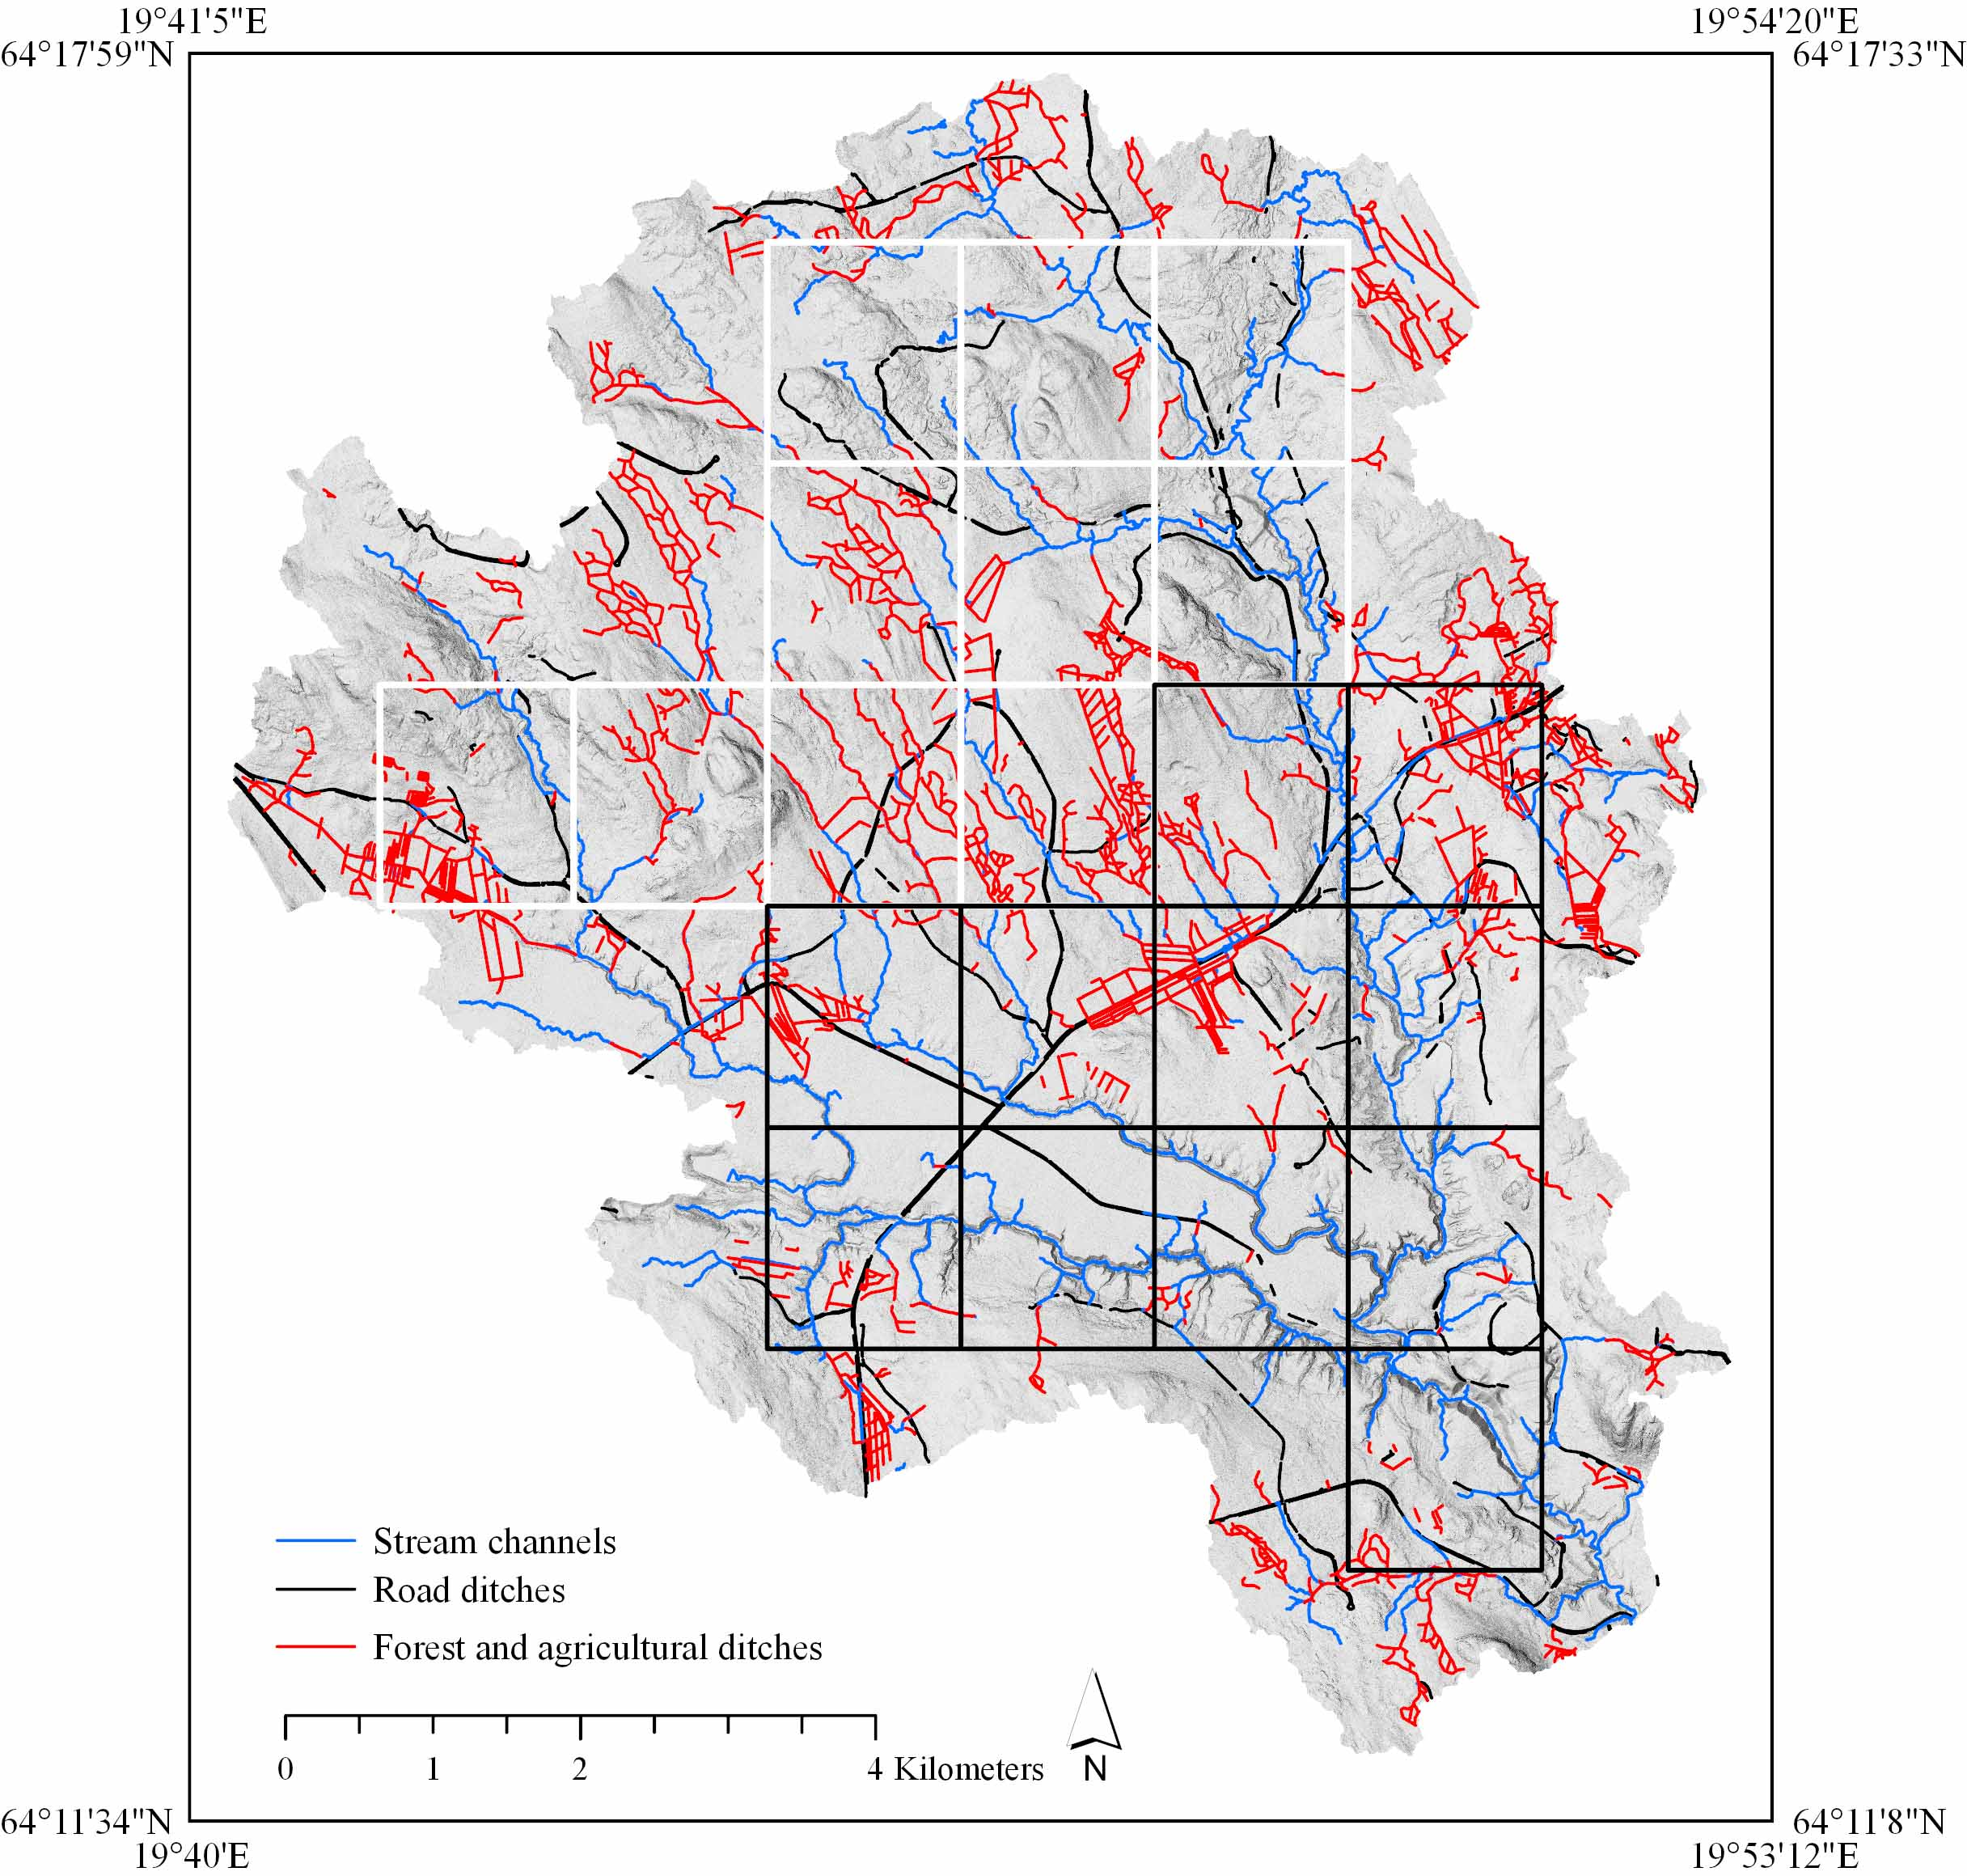
\includegraphics[width=1\linewidth]{./images/Krycklan_lo.jpg}
    \caption{Map of Krycklan showing ditches and stream channels, as well as our division into 21 subsections. The 10 subsections with a white border were used for developing input variables and optimising parameters before the experiment. The 11 subsections with a black border were used in the experiment for evaluation with 11-fold cross validation. Each rectangular subsection represents $2997 \cdot 2620$ pixels (roughly 196 hectare).}
    \label{fig:swedenkrycklan}
\end{figure}

From the ditch mapping, the vector layer was rasterised so that it could be compared to the automatically derived ditches from the $0.5*0.5$ m DEM. Our field observations have shown that the  width of most ditches within the catchment ranges between 0.5 and 3.5 m. To ensure that the model received all ditch pixels correctly in the training phase, we widened the ditches so that all pixels within a radius of three pixels (1.5 metres) of the vectors were labelled as ditch pixels. \hyperref[fig:ditchpreprocess]{Figure} \ref{fig:ditchpreprocess} \hyperref[fig:ditchpreprocess]{a} shows the ditches rasterised from vectors and \hyperref[fig:ditchpreprocess]{Figure} \ref{fig:ditchpreprocess} \hyperref[fig:ditchpreprocess]{b} shows the ditches after widening. The data in \hyperref[fig:ditchpreprocess]{Figure} \ref{fig:ditchpreprocess} \hyperref[fig:ditchpreprocess]{b} is the labelled data that was used to train the machine learning models. The ditches all have a generalised width based on a perceived average of ditch width in the area. Due to all ditches varying in width, it was impossible to produce a perfect representation of each ditch. However, this made for a good compromise for the average ditch.

Because our priority was to detect ditches, rather than accurately detecting each pixel labelled as a ditch, some adjustments were made when producing the prediction results. The dataset was divided into a lower resolution grid of $6*6$ pixels (9 $m^2$) for each grid. Each grid cell that contained at least 25\% ditch pixels was then labelled as a ditch, see \hyperref[fig:ditchpreprocess]{Figure} \ref{fig:ditchpreprocess} \hyperref[fig:ditchpreprocess]{c}. This layer was used to ground-truth the machine learning models.

\begin{figure} [htb!]
    \centering
    \subfigure[]{
        \resizebox*{4.5cm}{!}{\includegraphics{./images/publ_ditch_preprocess_A_lo.jpg}}}\hspace{5pt}
    \subfigure[]{
        \resizebox*{4.5cm}{!}{\includegraphics{./images/publ_ditch_preprocess_B_lo.jpg}}}
    \subfigure[]{
        \resizebox*{4.5cm}{!}{\includegraphics{./images/publ_ditch_preprocess_C_lo.jpg}}}
    \caption{Processing of ditch labels. \textbf{a: }Rasterised ditches with a width of one pixel. \textbf{b: }Ditches after a widening process, seven pixels (3.5 metres) wide. Used as input when training the models. \textbf{c: }Ditches after a grid zone conversion. Used for evaluating the results from the ditch detector.} \label{sample-figure}
    \label{fig:ditchpreprocess}
\end{figure}

\subsection{Extracting ditches with digital terrain indices}
From the DEM, several digital terrain indices were calculated:
\begin{itemize} \label{data_attributes}

  \item \textbf{Sky View Factor} \newline
  The Sky View Factor is a digital terrain index with a value ranging from 0 to 1, representing how much of the sky that is visible from a certain point on the ground \citep{zaksek}. On an open field all of the sky would be visible, but at the bottom of a ditch much of the sky would be obscured, meaning low values would indicate ditches. The Sky View Factor was calculated in SAGA GIS, using a search radius of 10 metres to ensure that ditches were covered, and to not let steep hills close to ditches affect the results.

  \item \textbf{Impoundment Index}\newline
  The tool Impoundment Index in Whitebox Tools \citep{whiteboxtools} is a digital terrain index designed to serve as a measure of topographic incision and flow constriction. The index effectively maps the area and average depth of the reservoir that would be created by placing a dam of a user-specified length at each grid cell in the DEM. The tool can be tuned to output the flooded area or volume (in which case it highlights areas of flow constriction), or the average flooded depth (which seems to measure topographic incision). Additionally, the tool will output a 'dam height' raster that is particularly useful for mapping channels, such as ditches. Here, we used dam height calculated with a dam length of 3 metres, to cover the entire ditch which is typically not wider than 3 metres. Typical false positives with this method are natural stream channels with a clear incised channel.
  
  \item \textbf{High Pass Median Filter} \newline
  High Pass Median Filters (HPMF) highlight ditches by indicating local depressions in the DEM. The algorithm operates essentially by subtracting the value at the grid cell at the centre of the window from the median value in the window. Negative values indicate depressions in the DEM, such as ditches. Typical false positives with this index are small hollows that also show negative numbers. HPMF was calculated using Whitebox Tools \citep{whiteboxtools} with a window size of $4.5 * 4.5$ m. 

    \item \textbf{Slope} \newline
    The Slope index represents the degree of slope at a certain point, with a value ranging from $0^{\circ}$ to $90^{\circ}$. It was calculated on the 0.5 m grid, using ArcGIS \citep{EsriArcGisBook}. This index contains no information about the direction of the slope.
\end{itemize}

\subsubsection{Thresholding the digital terrain indices}
To benchmark our method against a non-machine learning method, we binarised the original four digital terrain indices using thresholds. Different threshold values were tested and the value that yielded the highest Cohen's Kappa score for each respective index was chosen. This test was conducted for the 11 subsections described in \ref{trainingvalidationdatasets}. The Sky View Factor index was classified to only include values below 0.955, the Impoundment Index Dam Height using values above 0.27 $m$, the HPMF index using values below -0.18 m, and the Slope index using values above $14 ^{\circ}$ (Table 2). 

\subsection{Data preparation}

\subsubsection{Processing the digital terrain indices}
We examined how different  input variables affected the prediction of the machine learning models. Several possible data manipulation methods could theoretically produce a better prediction. To improve the prediction, steps were taken where neighbouring pixels were included to give a representation of the area surrounding a specific pixel, similar to the approach of \citet{roelens}. 

The digital terrain indices provided a satisfactory foundation for the models, but lacked in the generalisability of their predictions. More diverse input variables were extracted using simple statistical aggregates such as mean, median, min, max, and standard deviation. Using these statistical aggregations with the help of neighbouring areas around pixels aided in pruning pixels with outlier values, often smoothing out the data to represent ditches more accurately on a per-pixel basis. These variables were calculated by gathering all data points in different circular radii around the studied pixel, before computing one of the statistical aggregations (\hyperref[fig:features]{Figure} \ref{fig:features}: \hyperref[fig:features]{b}, \hyperref[fig:features]{c}, \hyperref[fig:features]{f}, and \hyperref[fig:features]{g}).

In addition to the general input variables, a number of custom input variables were also developed.  Some of these custom variables were produced by statistical aggregation of multiple indices whereas in some cases, they were generated by using thresholds to exclude, lower, or amplify the values of pixels that indicated ditches or non-ditches (\hyperref[fig:features]{Figure} \ref{fig:features}: \hyperref[fig:features]{d} and \hyperref[fig:features]{h}).

Both HPMF and Sky View Factor were used with the image processing \textit{gabor filter}, which can be used to detect lines of a certain orientation in an image \citep{gabor}. 30 Gabor filters which were rotated in different angles and with different frequencies were combined to detect lines, amplifying ditches by utilising the fact that ditches have a linear elongated shape (\hyperref[fig:features]{Figure} \ref{fig:features}: \hyperref[fig:features]{e}).

\label{impoundmentstreamremoval}
The raw Impoundment Index dam height was used to create a mask, attempting to mark out streams, but retain ditches. Only areas with a relatively high dam height, above 14 metres, which would indicate that these areas most likely contained streams, were masked out. After widening the resulting area, this mask was used to remove streams from all the aforementioned custom input variables, generating one new input variable from each. The features marked with \textit{streams removed} in \hyperref[featuretable]{Table} \ref{featuretable} make use of this filter (\hyperref[fig:features]{Figure} \ref{fig:features}: \hyperref[fig:features]{i}).

Overall, 81 input variables were extracted from the terrain indices. In a pilot study, we compared several different algorithms (Random Forests, Extreme Gradient Boosting, Naive Bayes, and Support Vector Machines), and it was found that Random Forests produced the most accurate results, here we therefore only present the results from the Random Forest model. We then conducted a sub-experiment to find the best input variables, as well as the optimal number of variables to use. The variable importance score in Random Forests was used to select the most important input variables and it was found that using the top 40 input variables produced the best results.

\begin{figure} [!htb]
    \centering
    \subfigure[]{
        \resizebox*{4cm}{!}{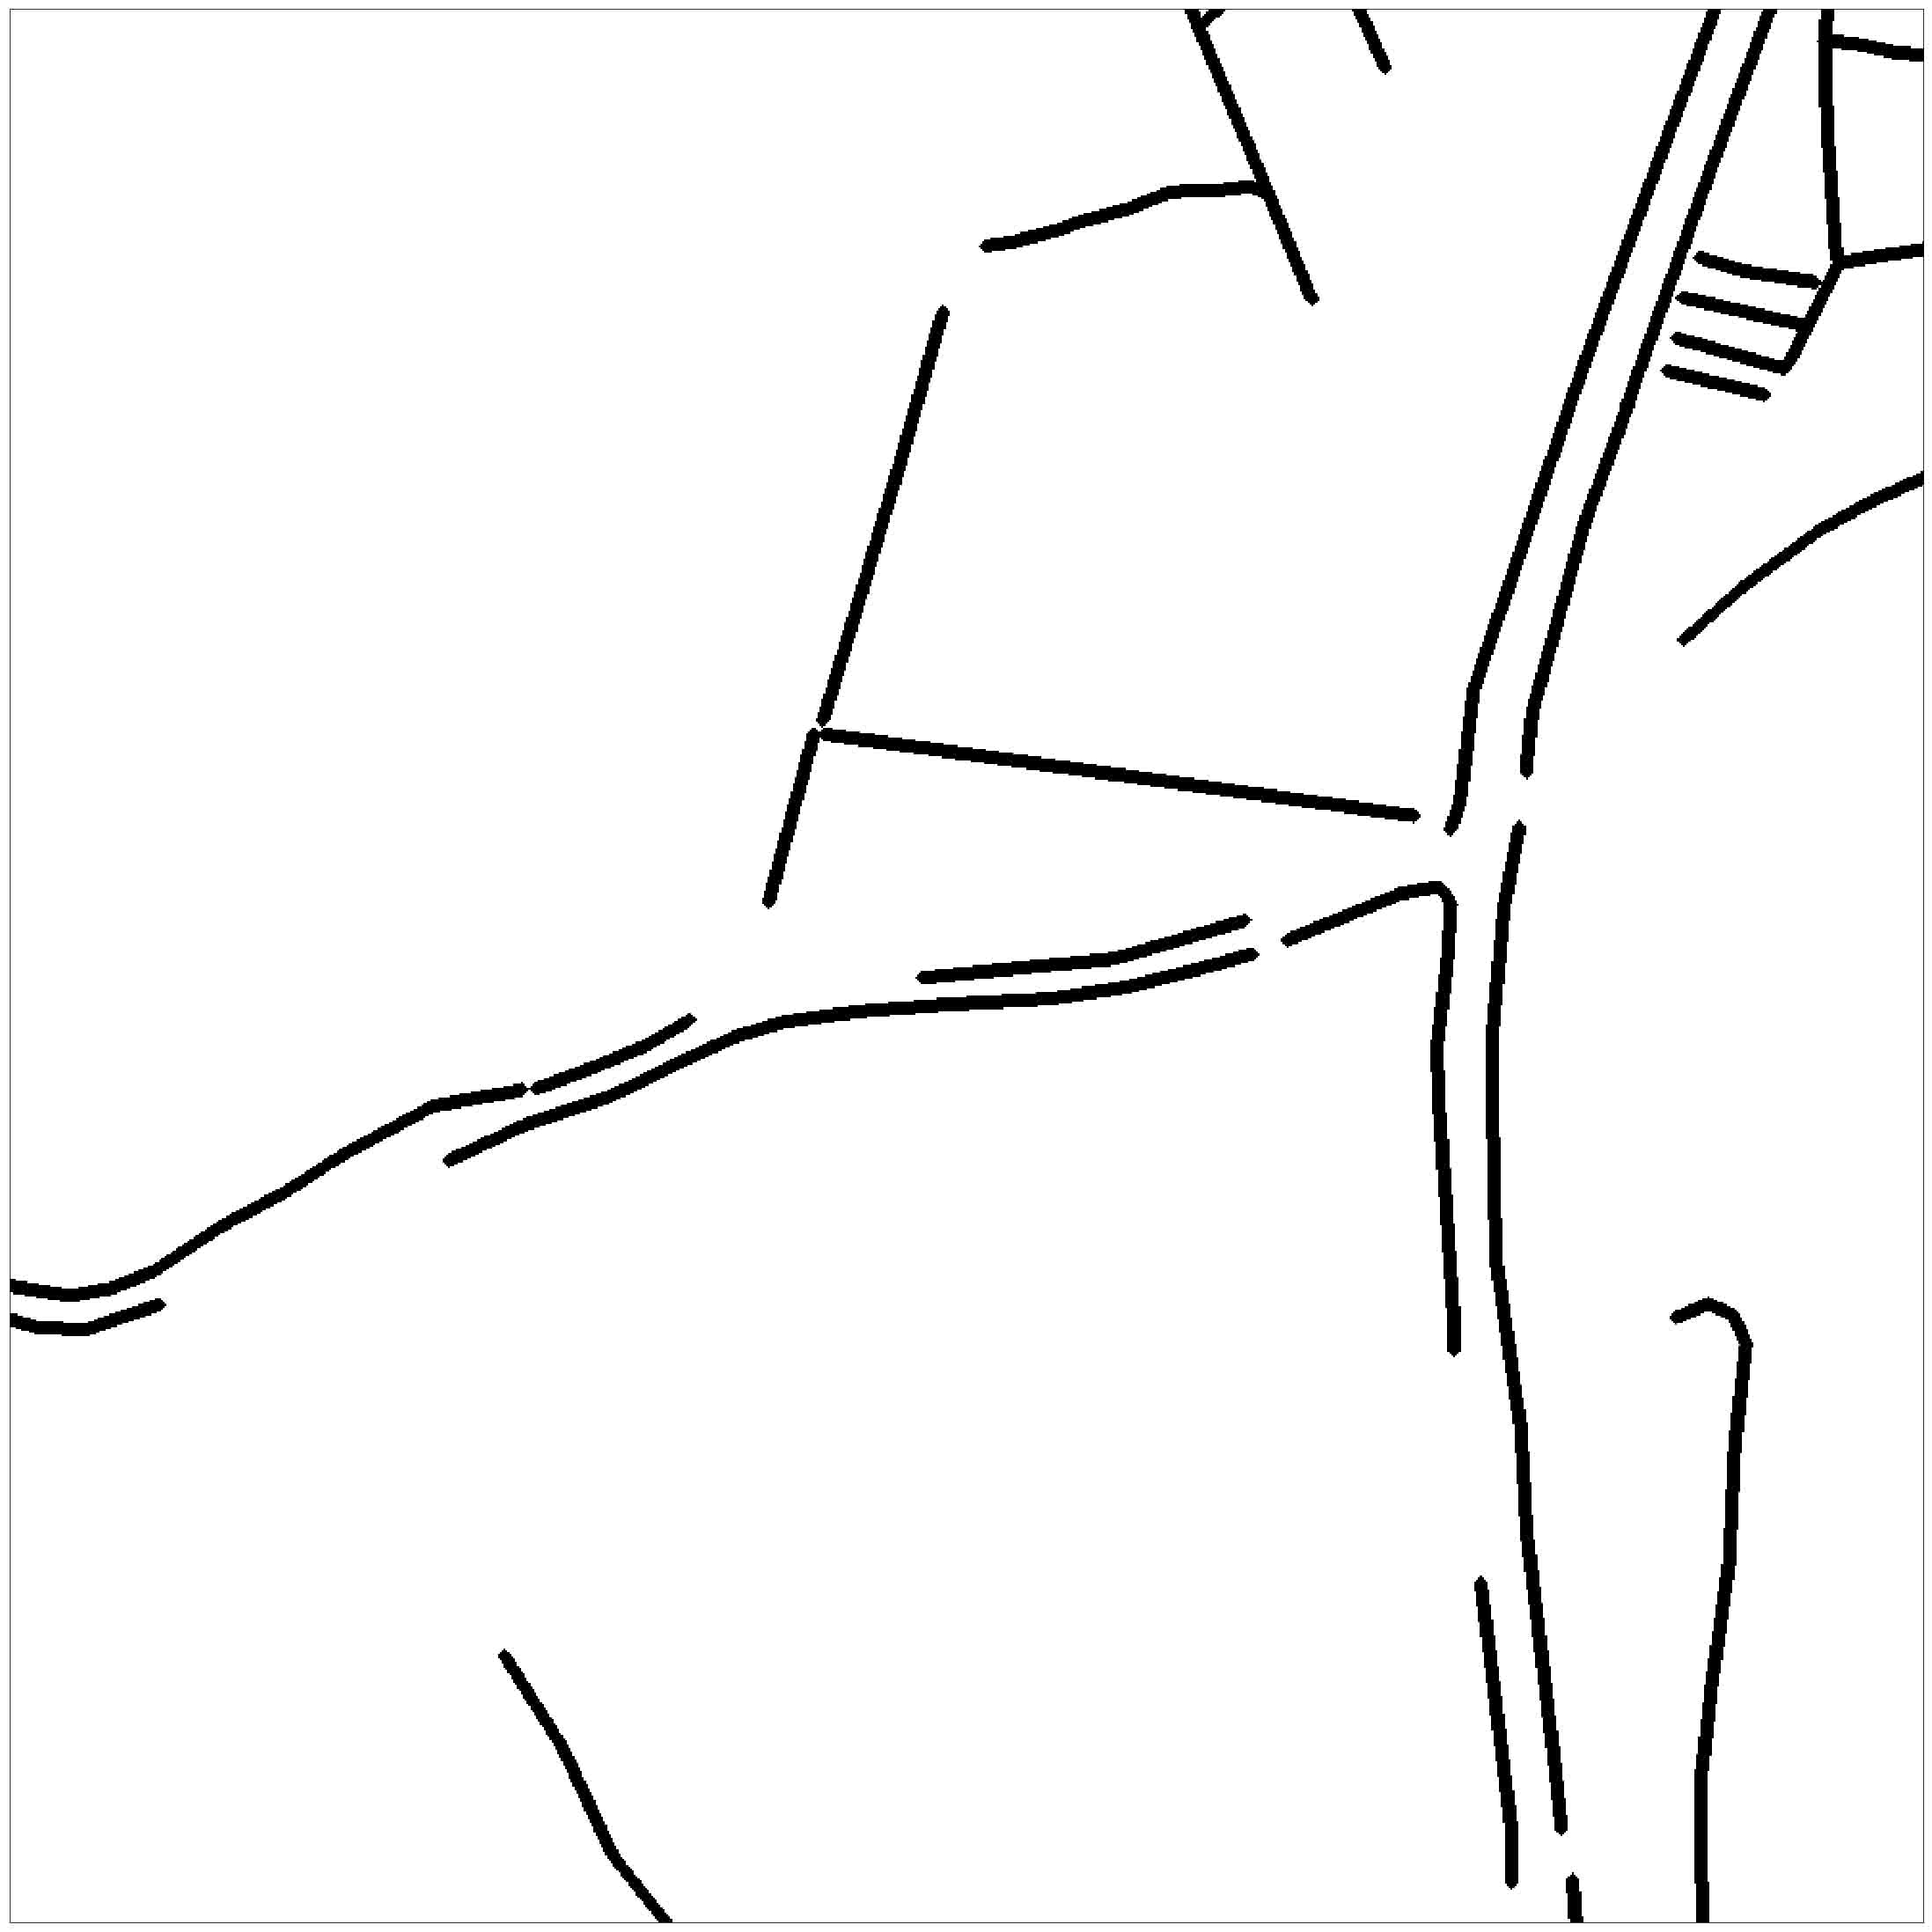
\includegraphics{./images/feature_a_lo.jpg}}}\hspace{5pt}
    \subfigure[]{
        \resizebox*{4cm}{!}{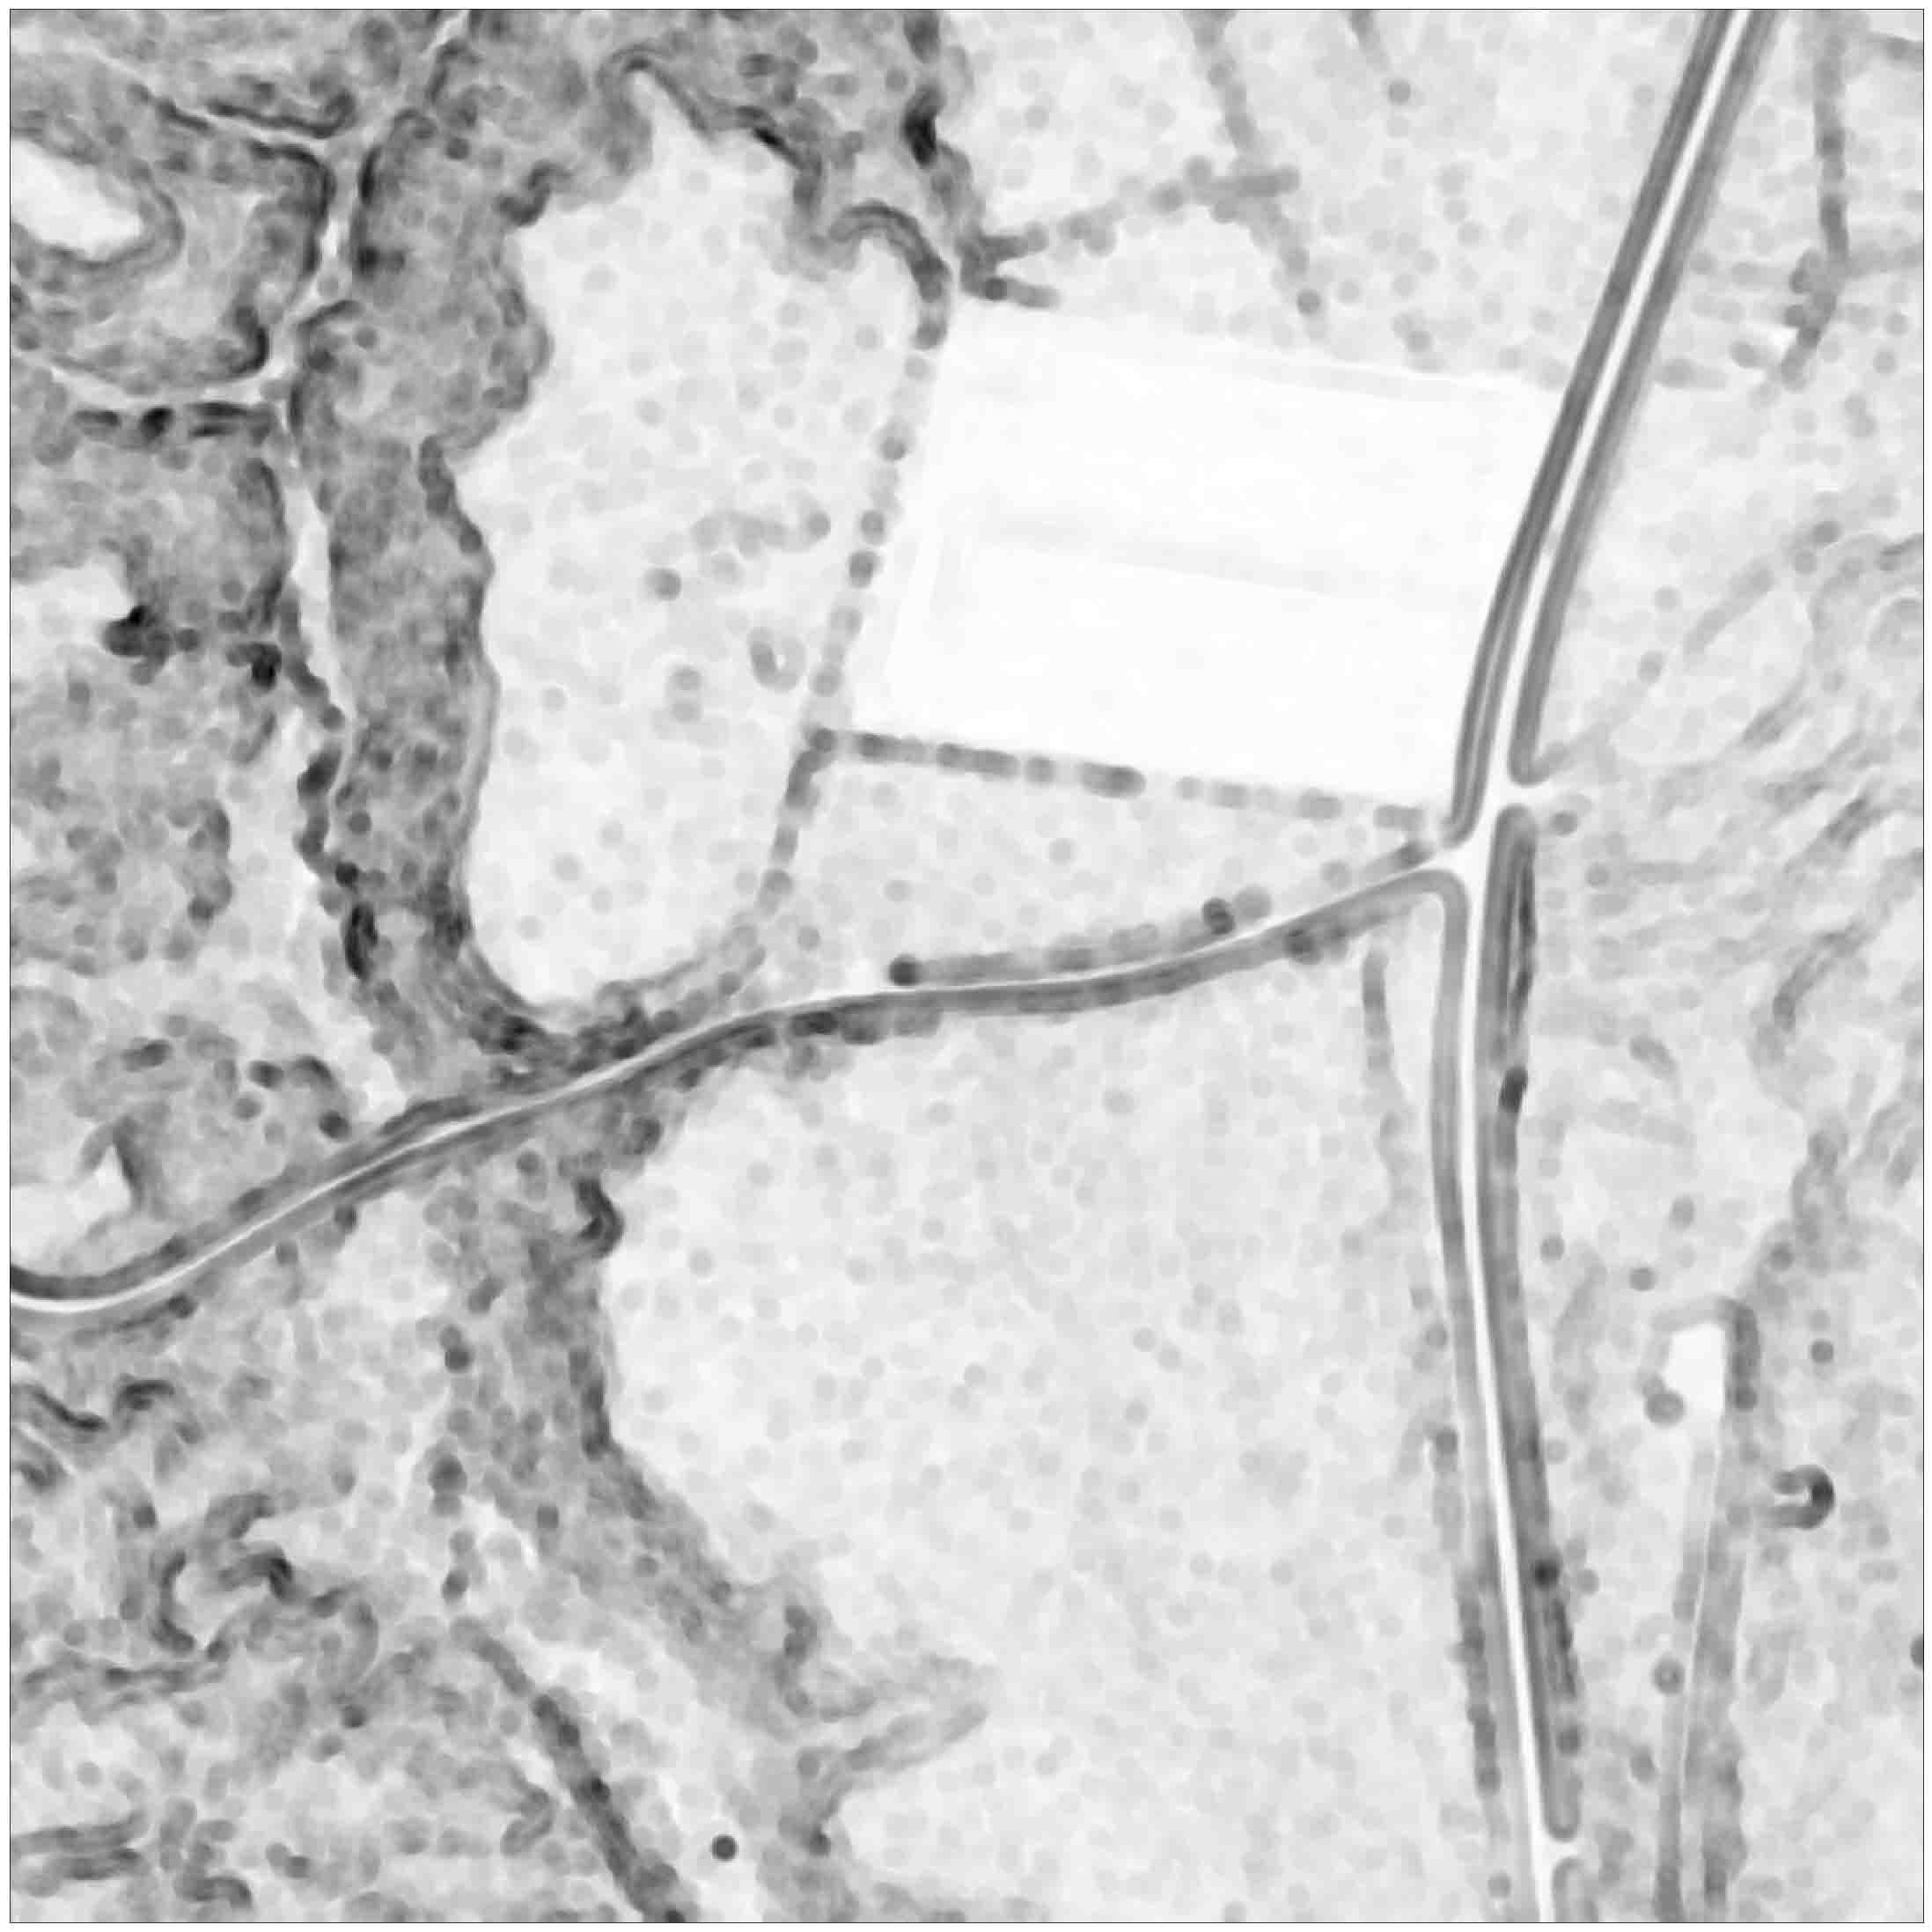
\includegraphics{./images/feature_b_lo.jpg}}}
    \subfigure[]{
        \resizebox*{4cm}{!}{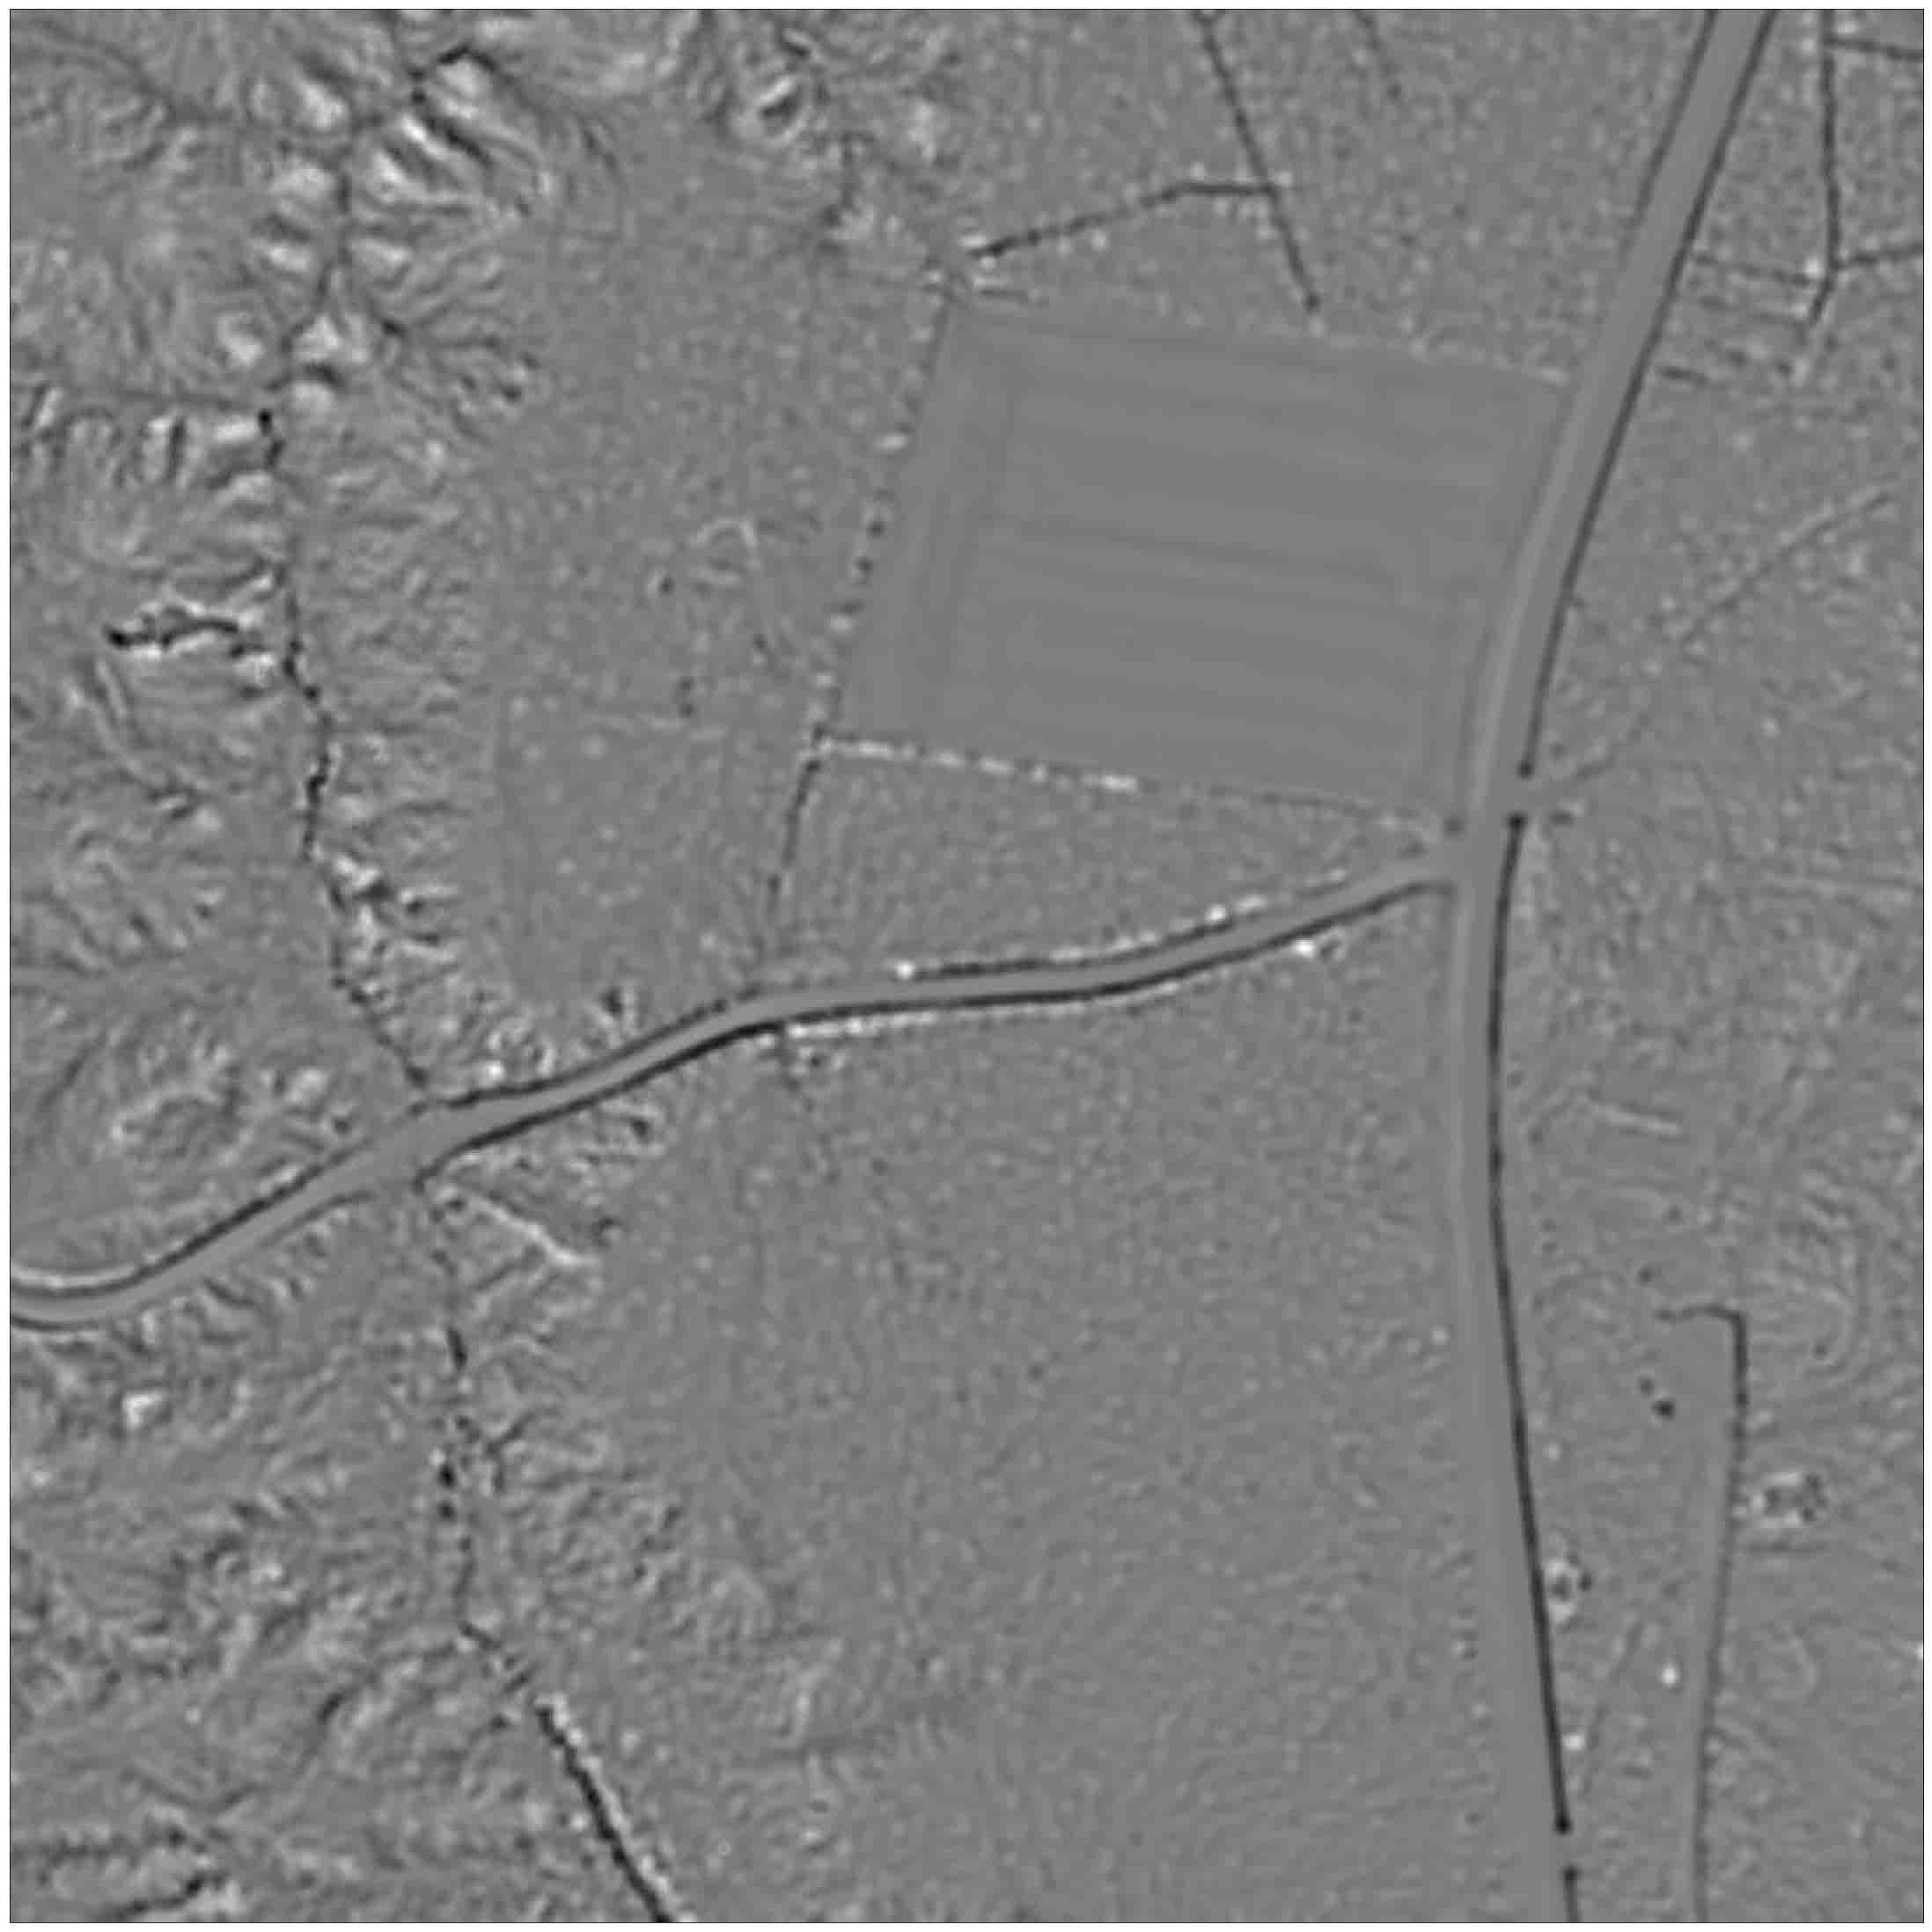
\includegraphics{./images/feature_c_lo.jpg}}}\hspace{5pt}
    \subfigure[]{
        \resizebox*{4cm}{!}{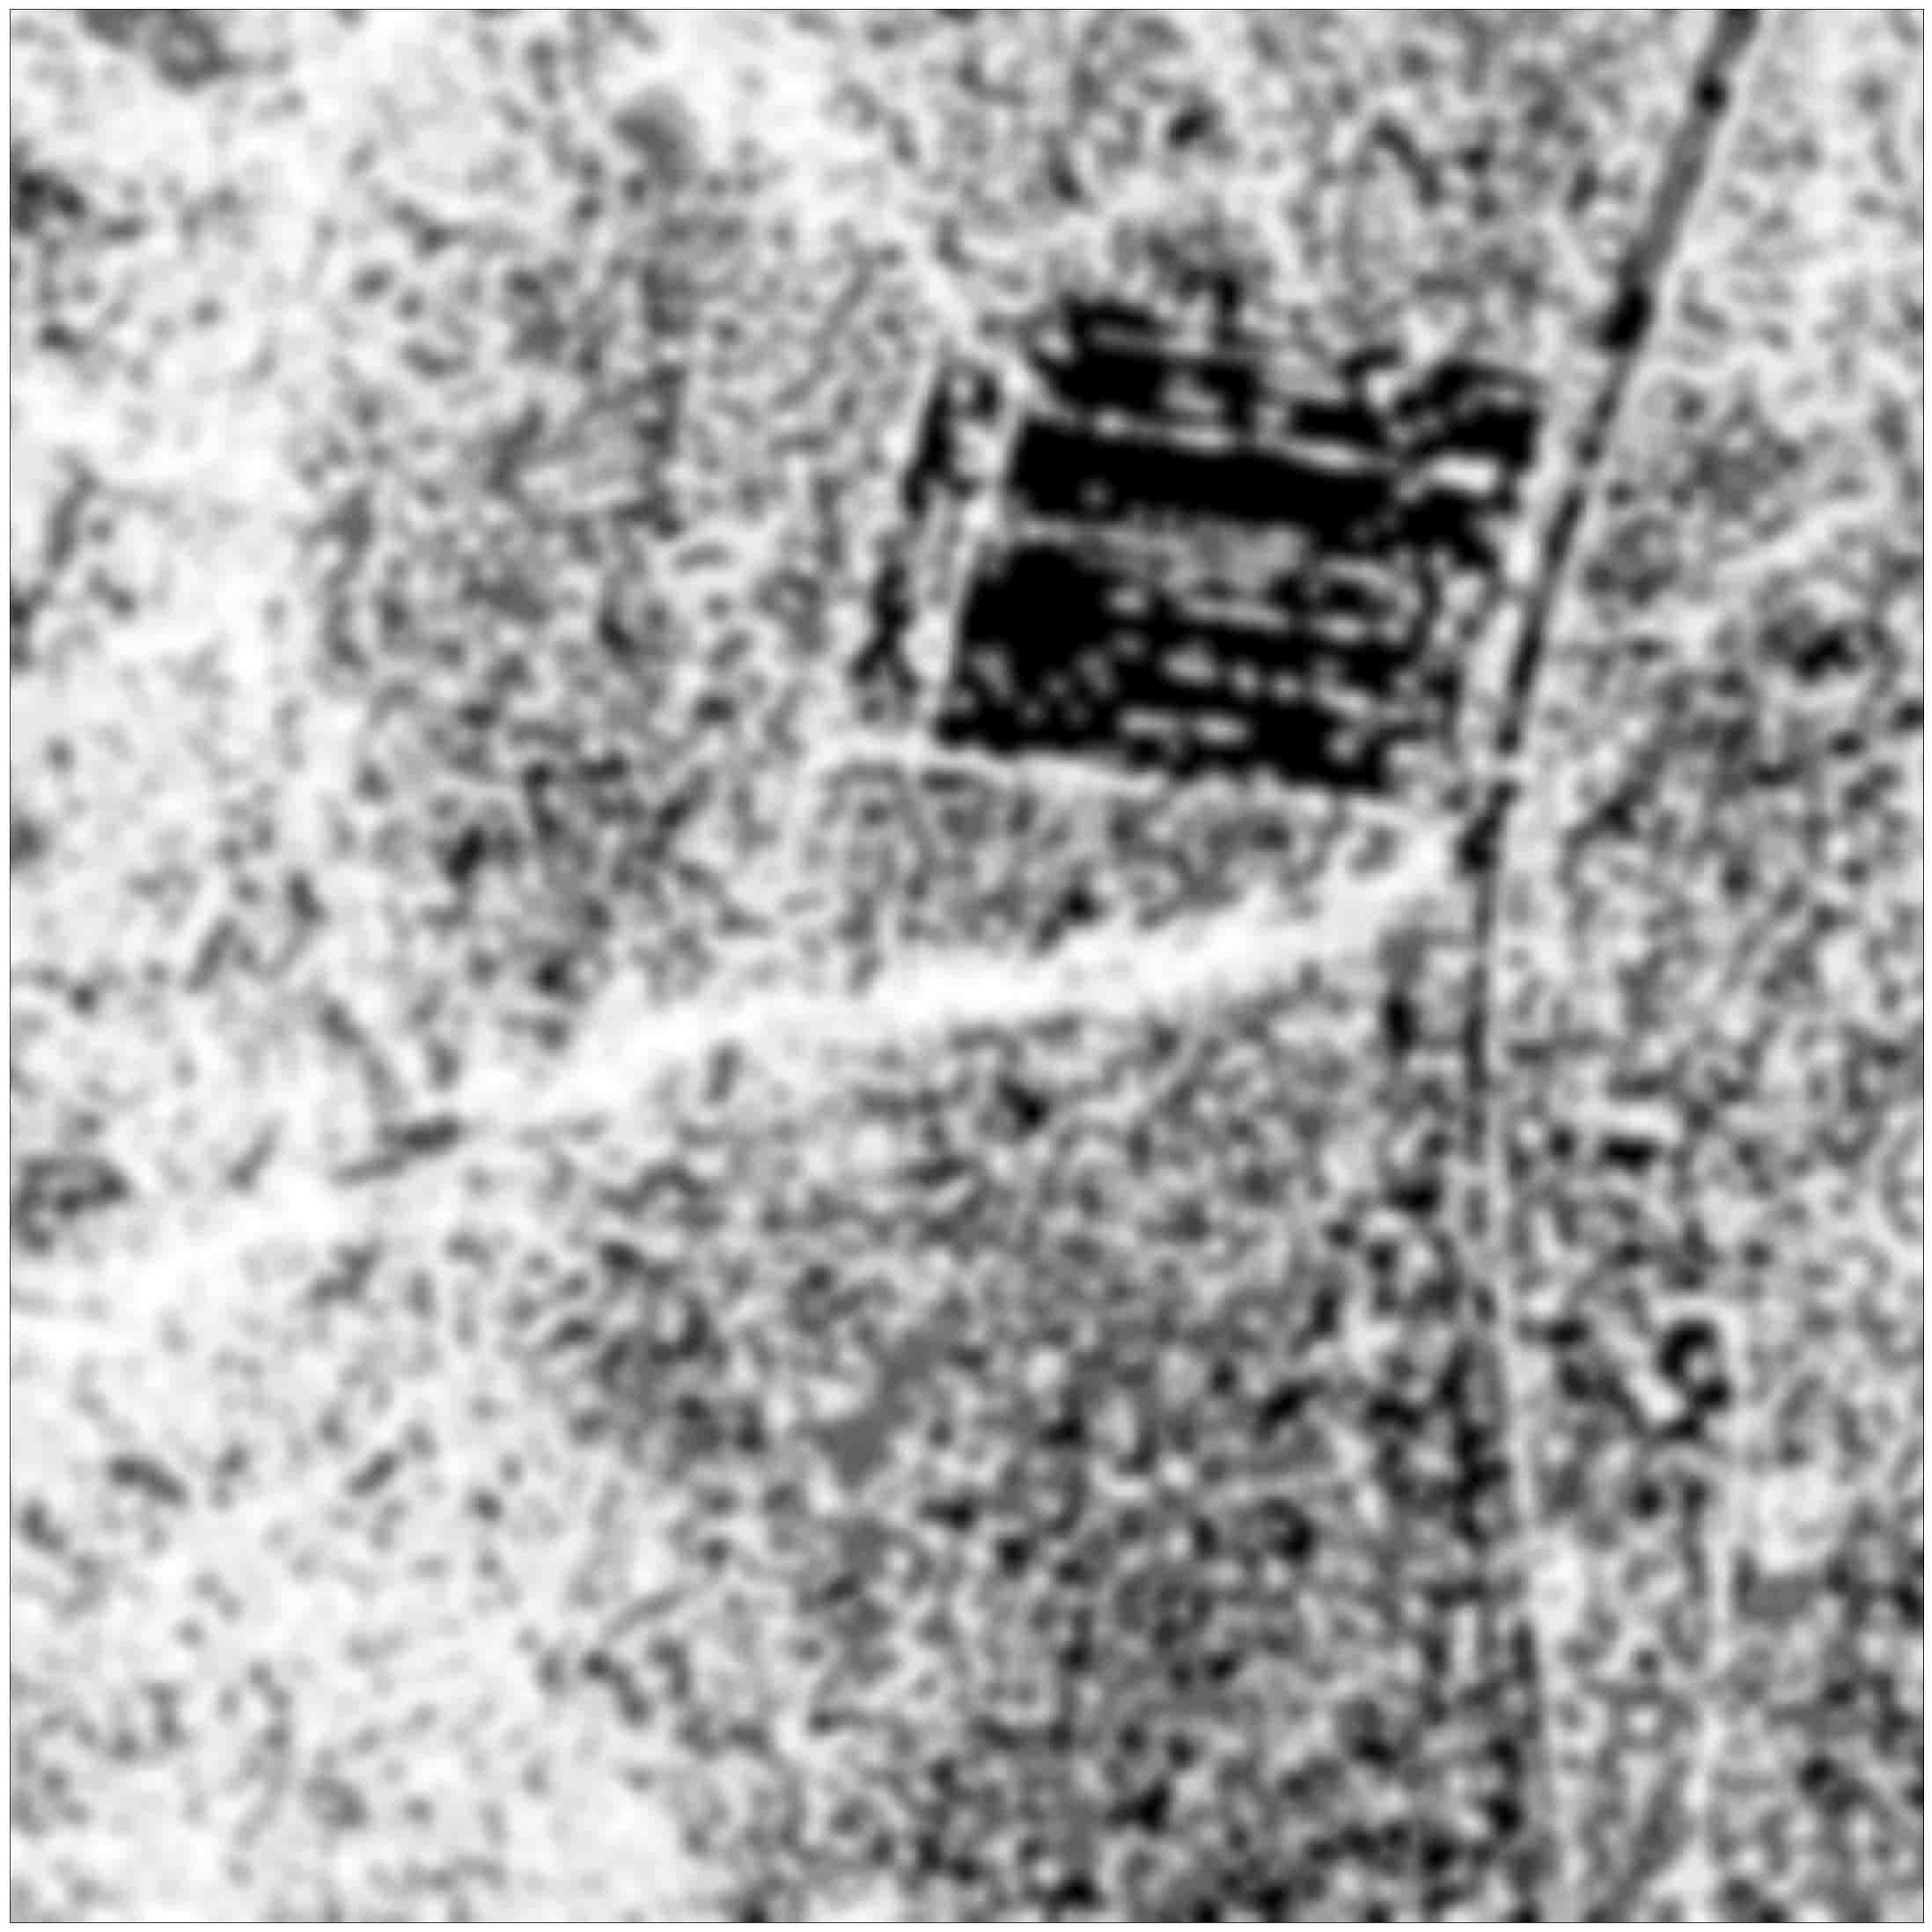
\includegraphics{./images/feature_d_lo.jpg}}}
    \subfigure[]{
        \resizebox*{4cm}{!}{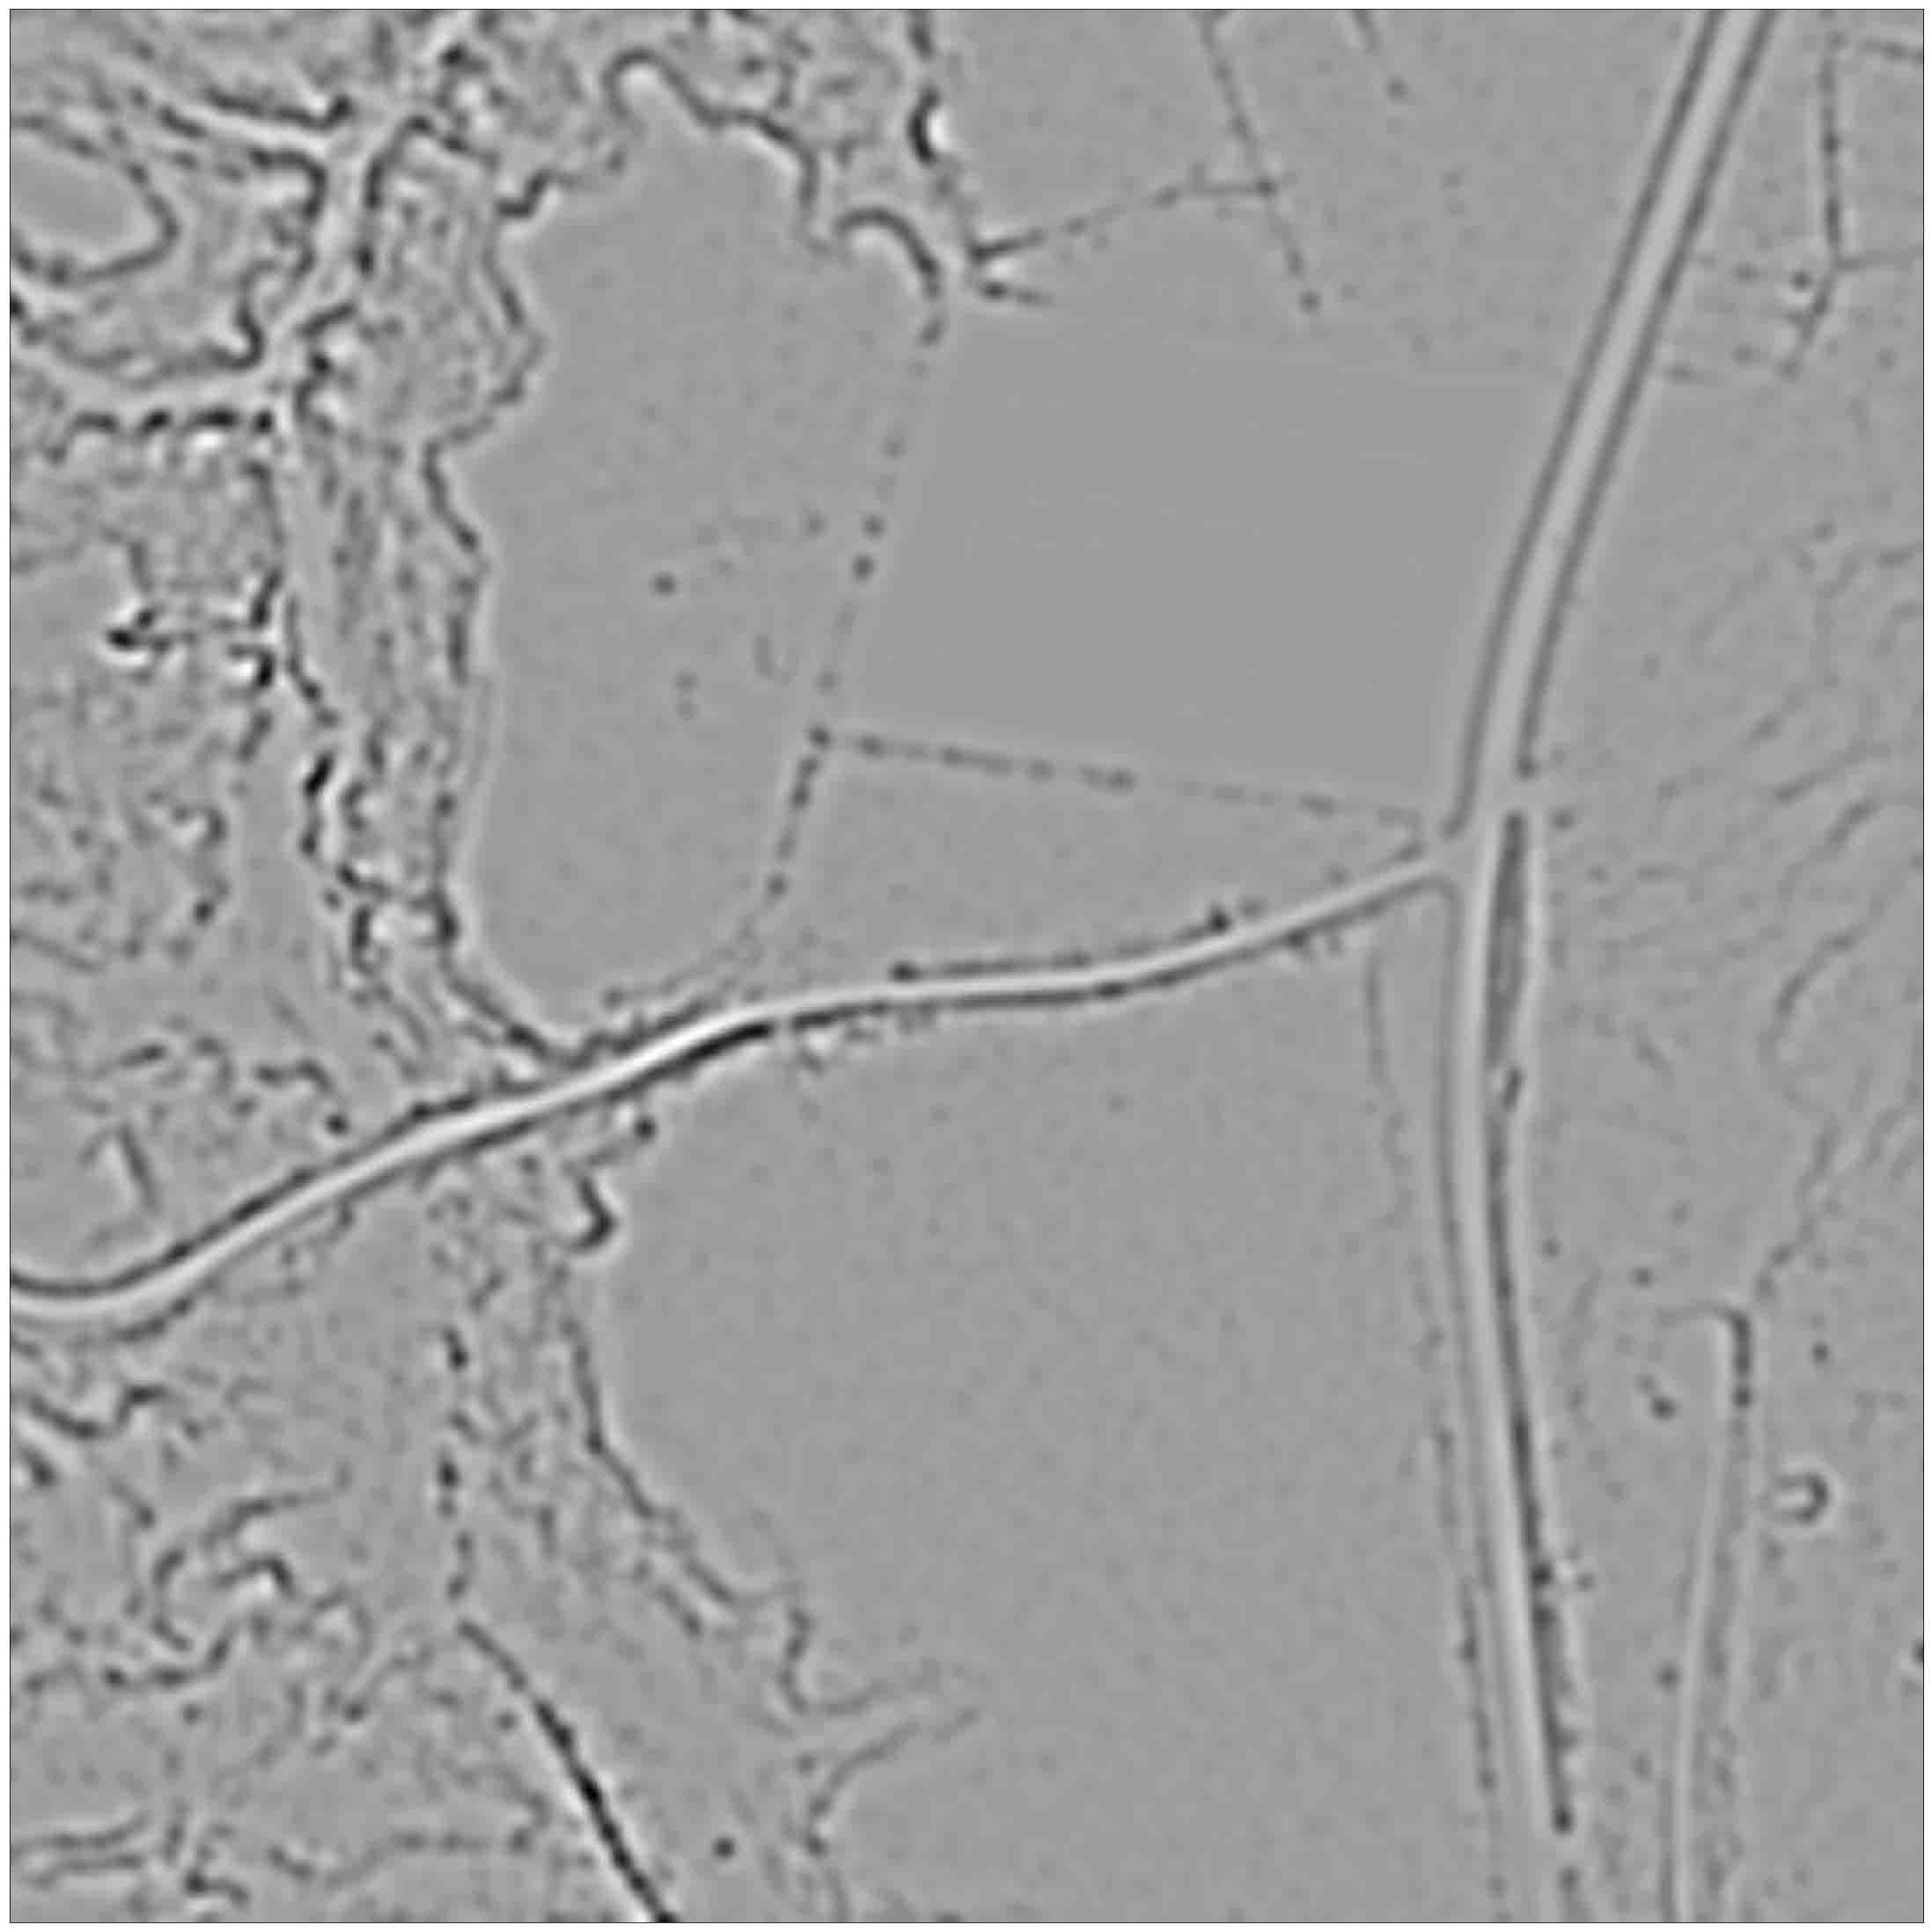
\includegraphics{./images/feature_e_lo.jpg}}}\hspace{5pt}
    \subfigure[]{
        \resizebox*{4cm}{!}{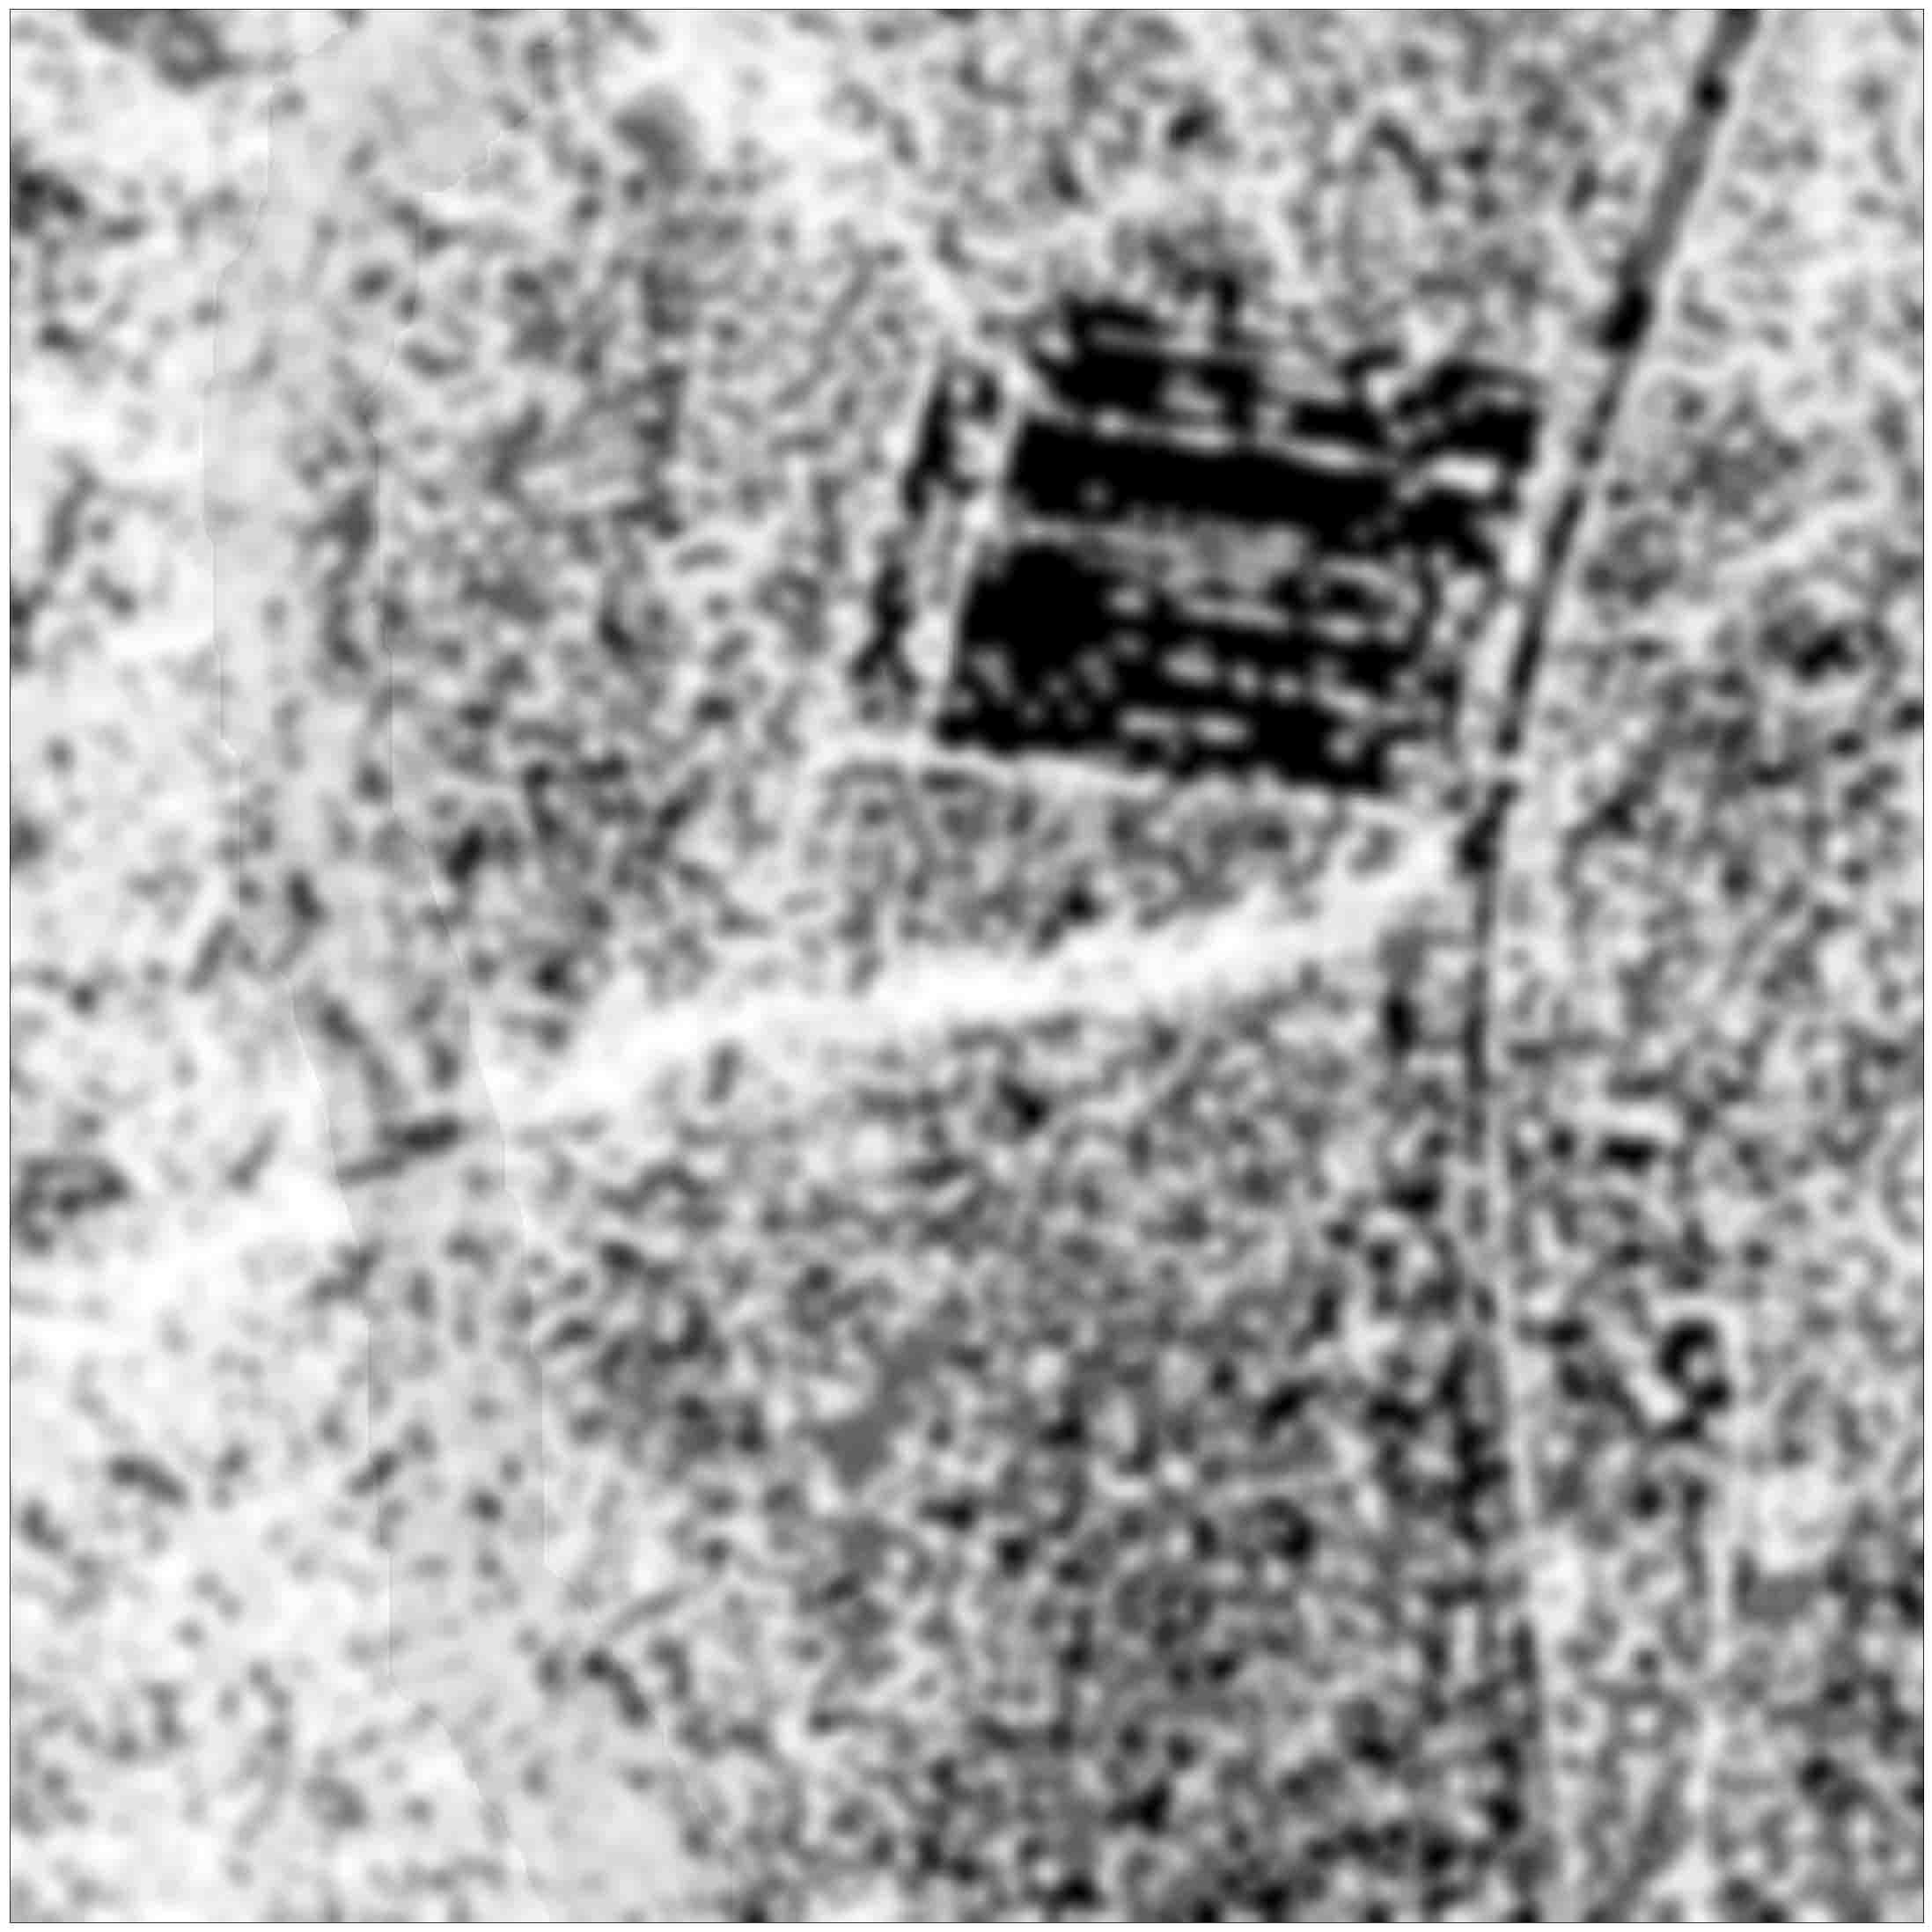
\includegraphics{./images/feature_f_lo.jpg}}}
    \subfigure[]{
        \resizebox*{4cm}{!}{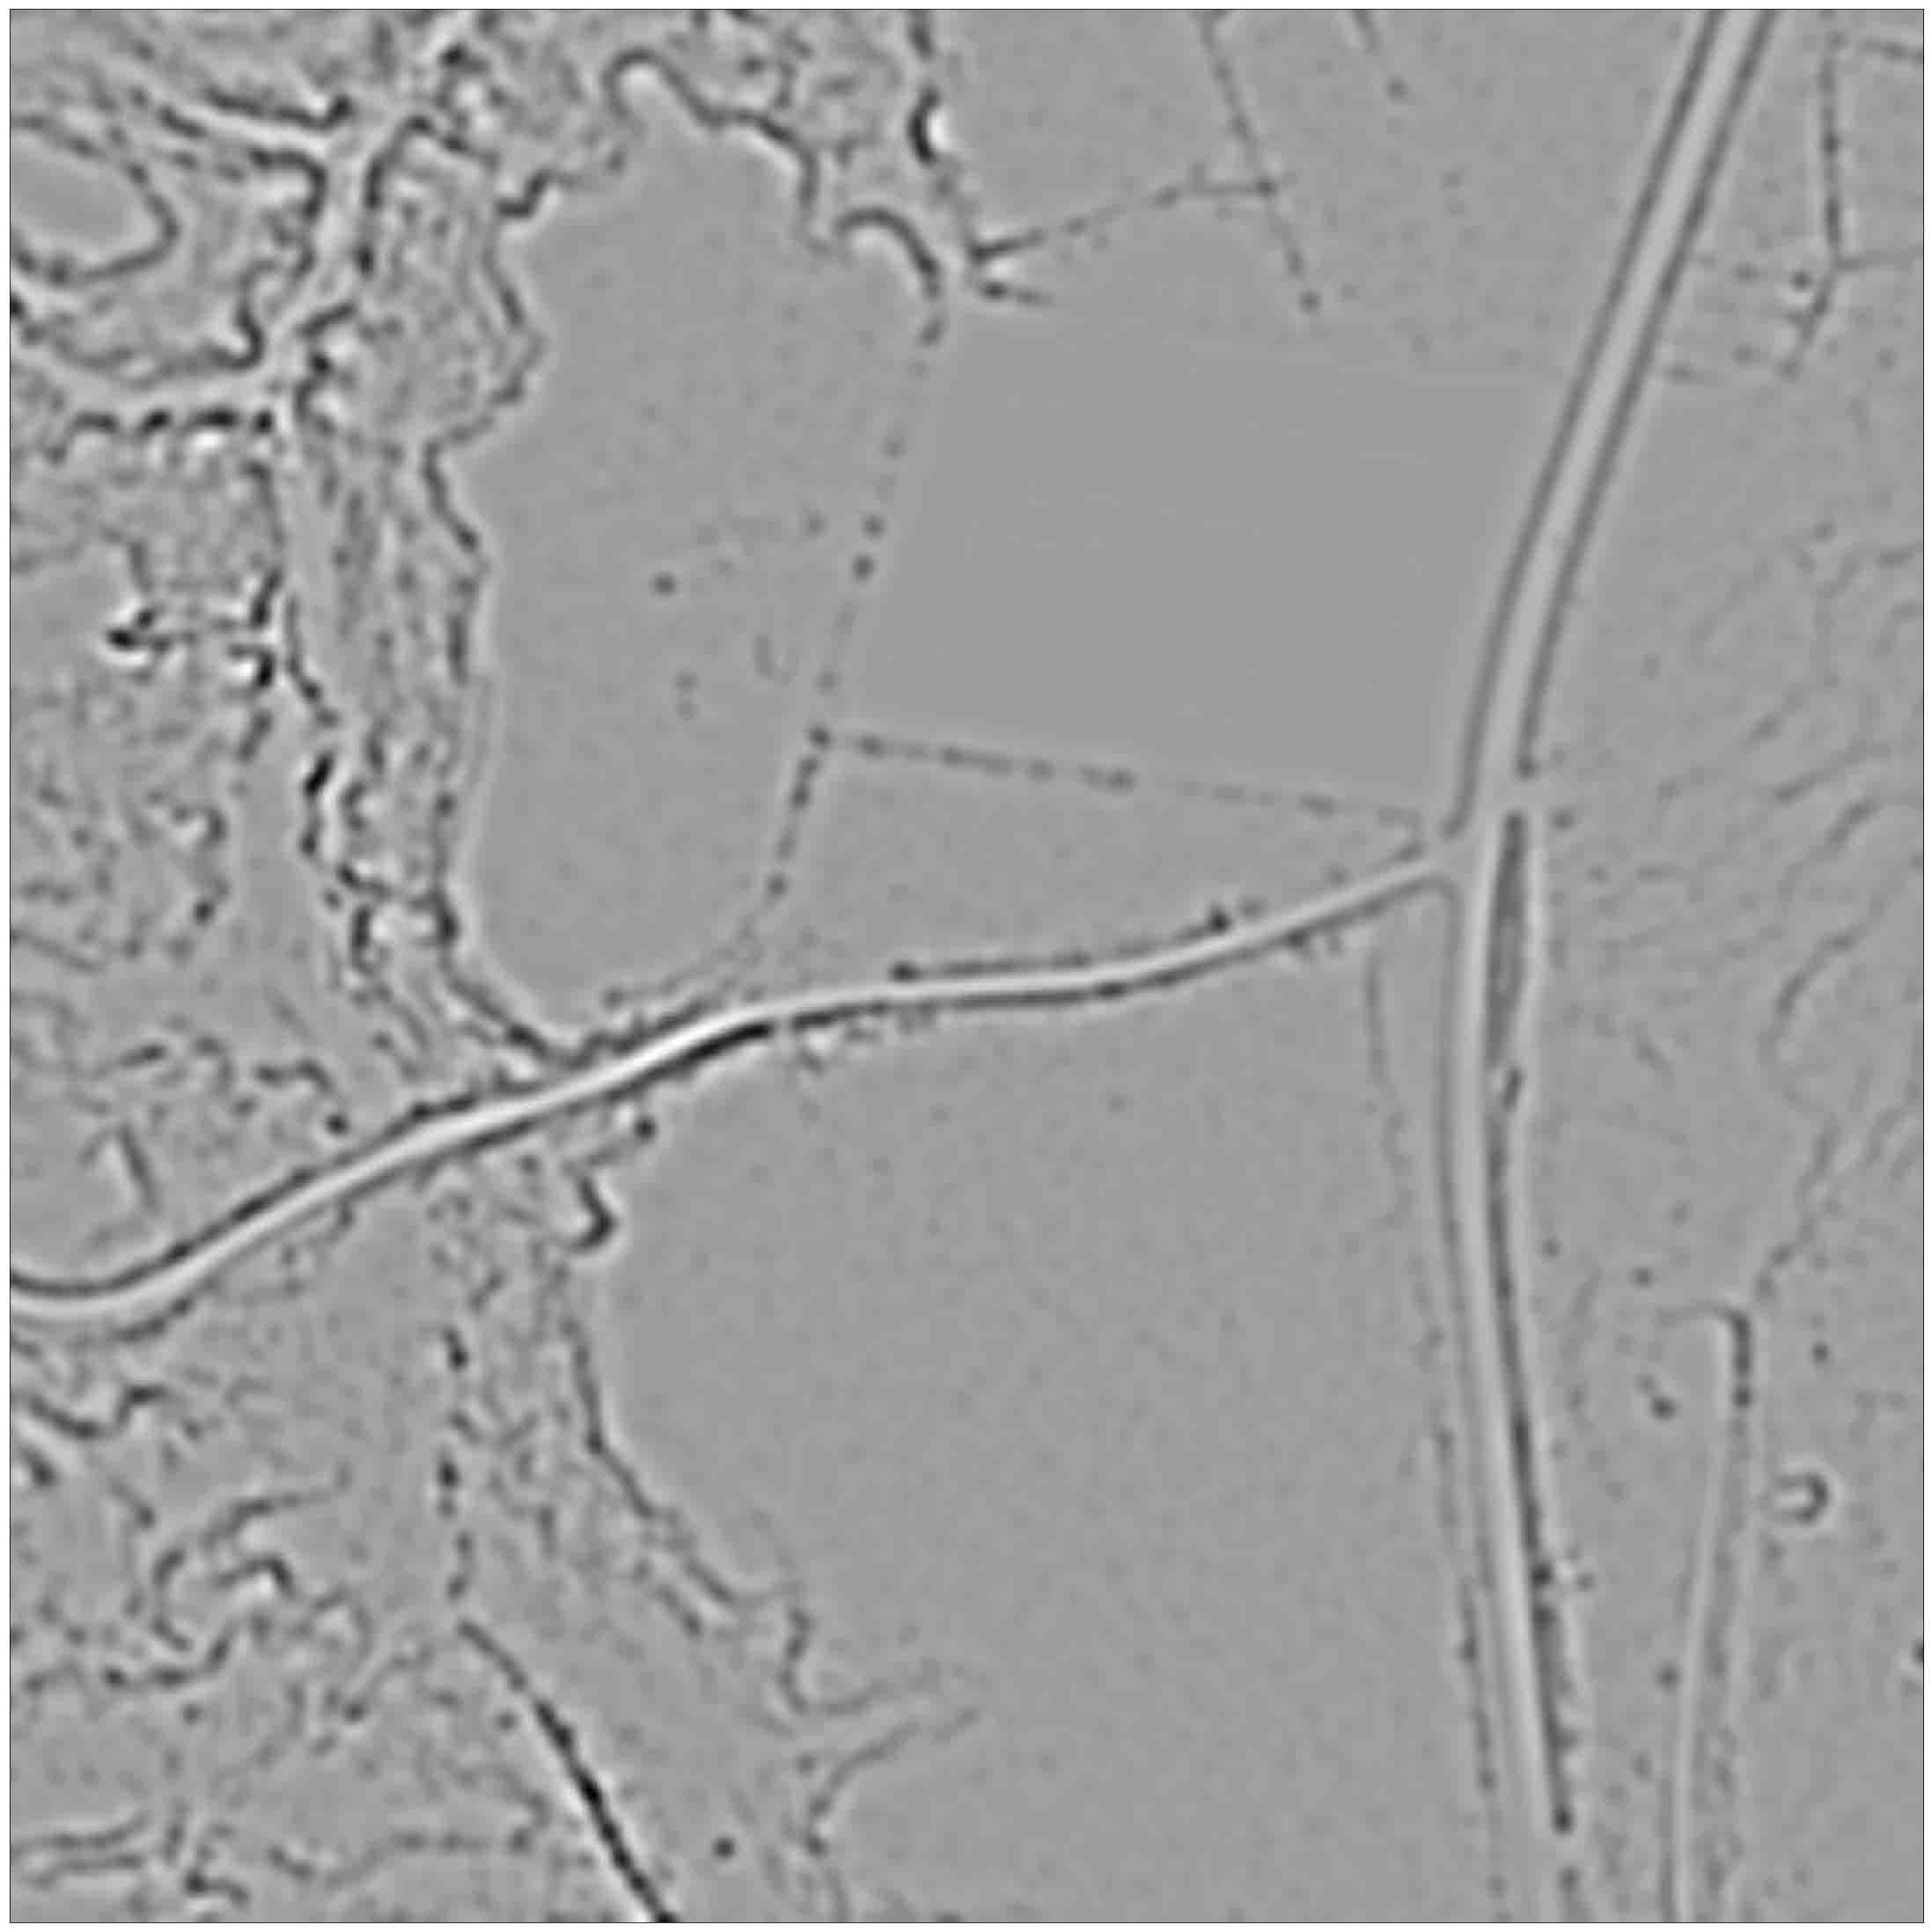
\includegraphics{./images/feature_g_lo.jpg}}}\hspace{5pt}
    \subfigure[]{
        \resizebox*{4cm}{!}{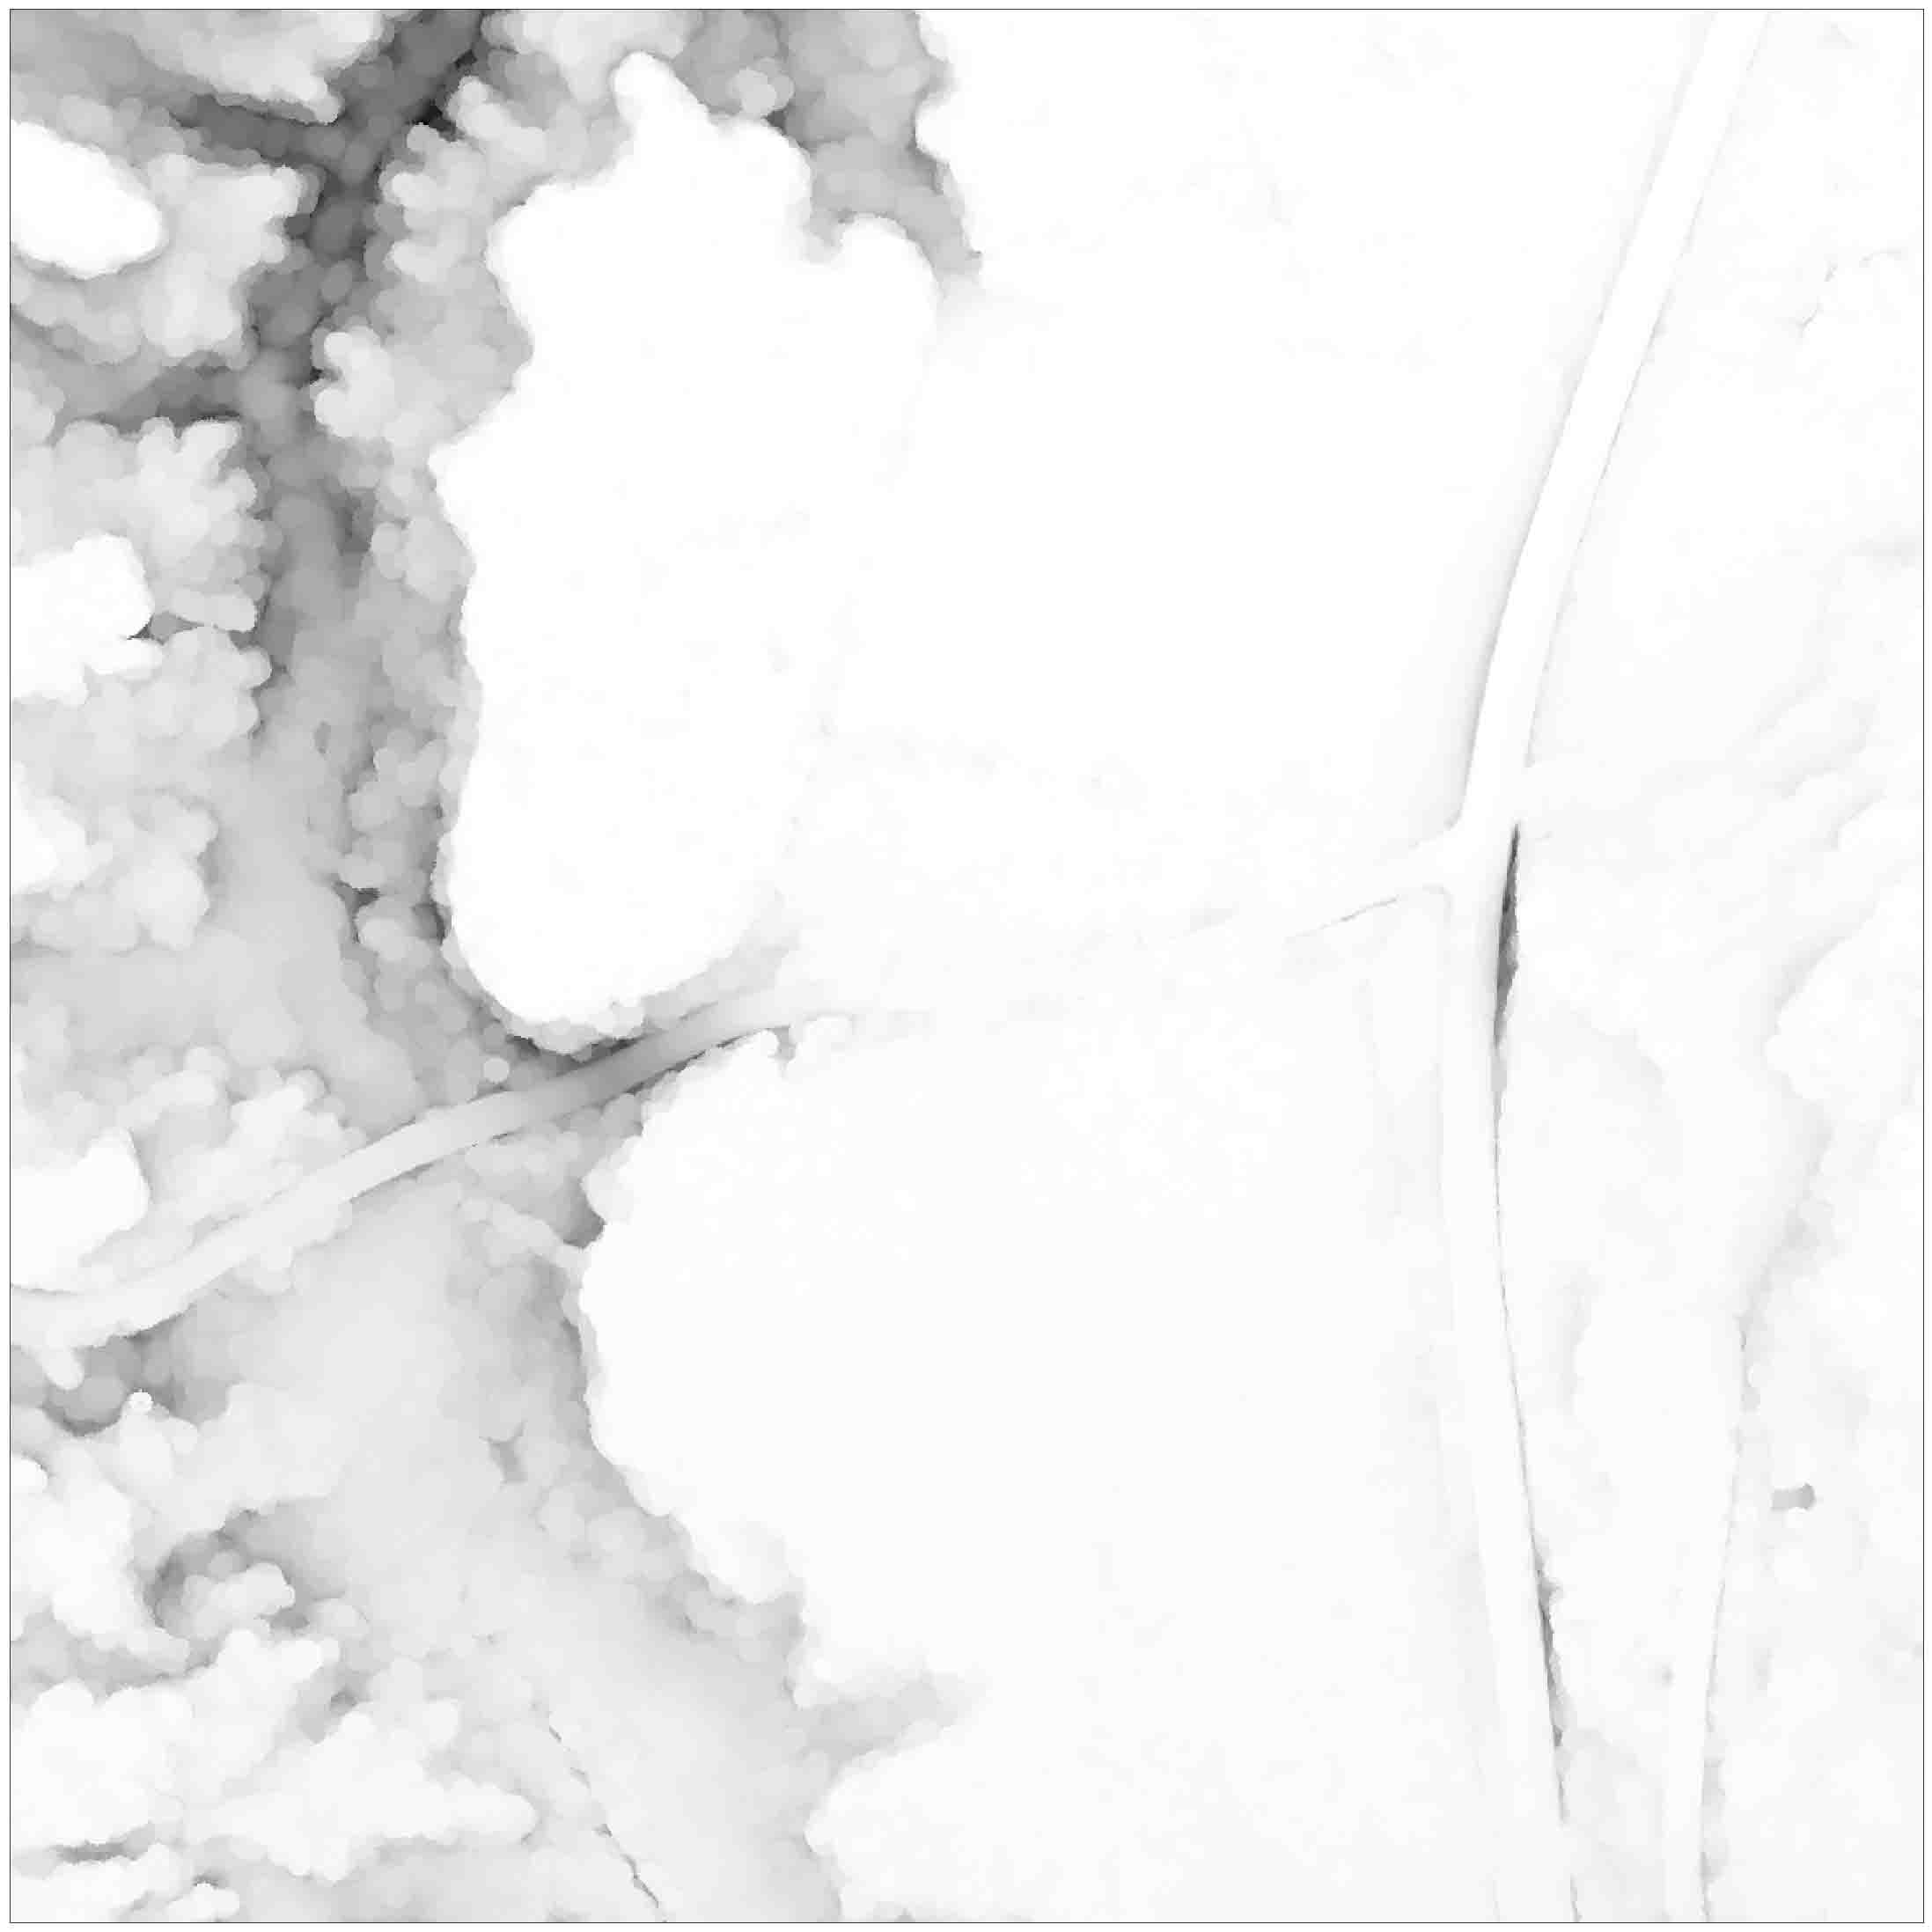
\includegraphics{./images/feature_h_lo.jpg}}}
    \subfigure[]{
        \resizebox*{4cm}{!}{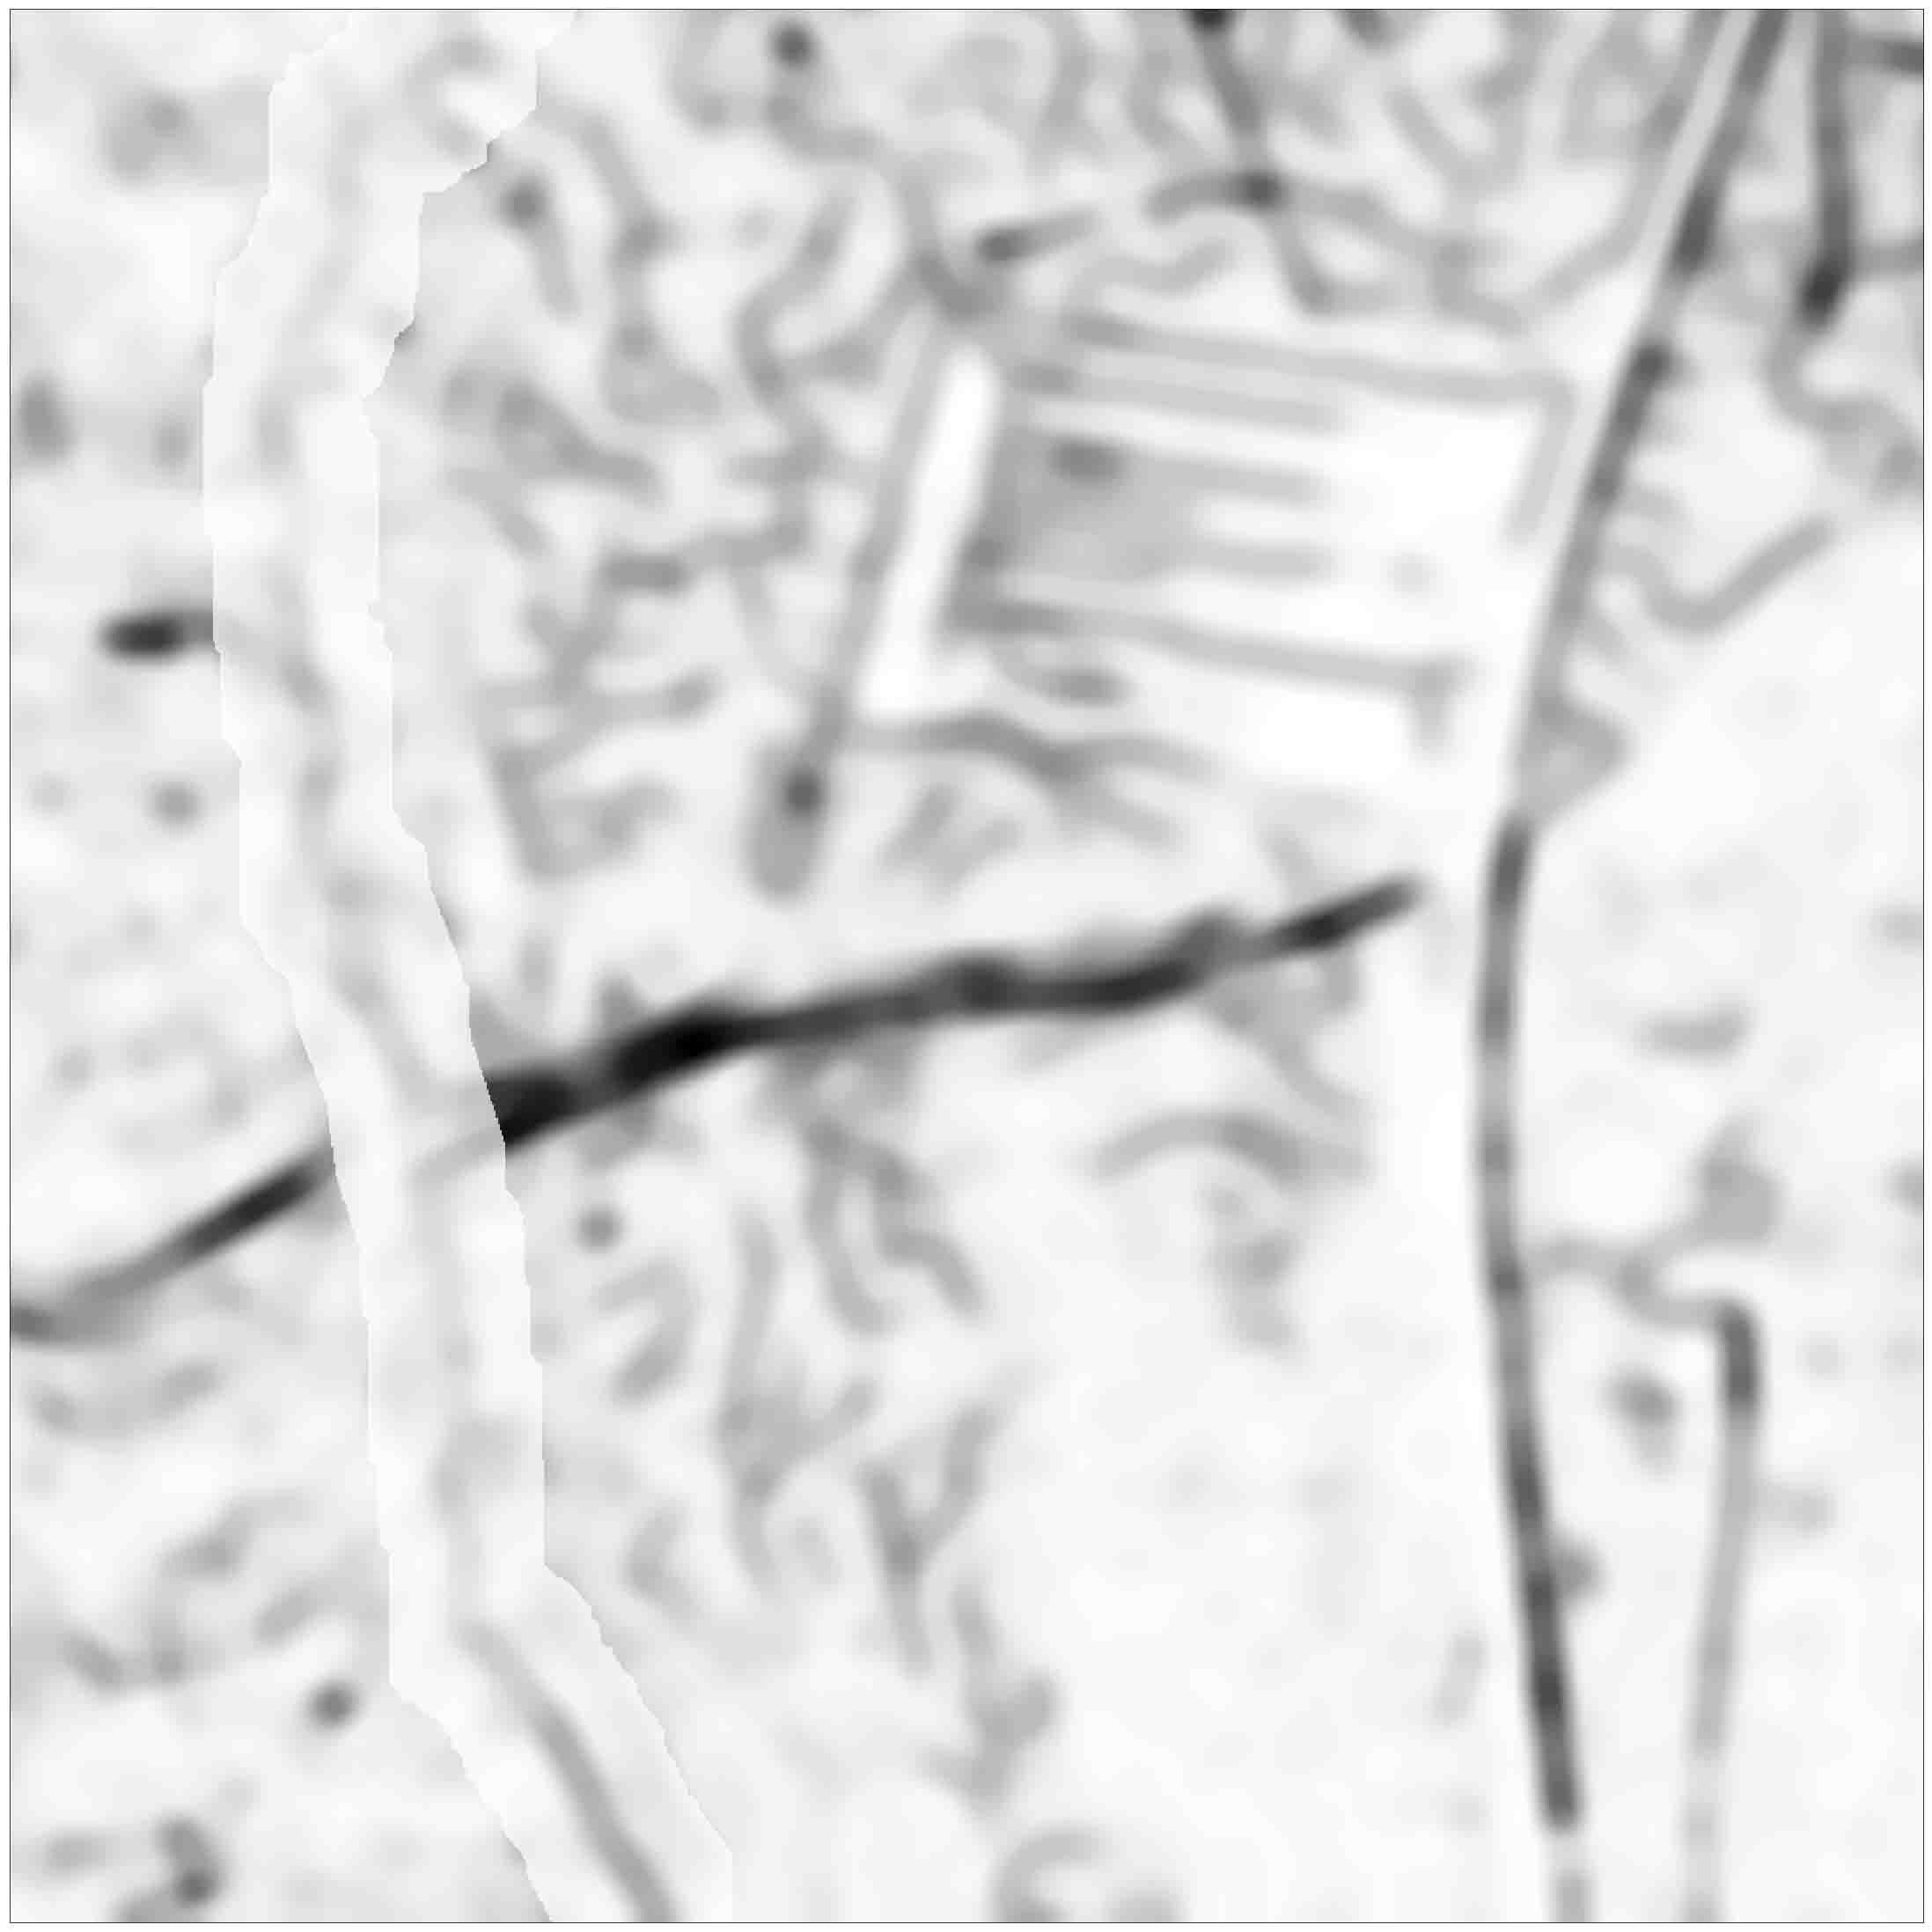
\includegraphics{./images/feature_i_lo.jpg}}}
    \caption{Example of 8 of the 40 input variables, in addition to ditch labels used by the models for a small sample area. The radii represents pixels with a 0.5 m resolution. \newline \textbf{a:} Labelled ditches, \textbf{b:} Slope standard deviation, radius 6, \textbf{c:} HPMF mean, radius 4, \textbf{d:} HPMF ditch amplification, \textbf{e:} Sky View Factor Gabor, \textbf{f:} Sky View Factor max, radius 6, \textbf{g:} Impoundment mean, radius 3, \textbf{h:} Impoundment ditch amplification, \textbf{i:} Impoundment ditch amplification - streams removed}
    \label{fig:features}
\end{figure}

\subsubsection{Training and validation datasets}
\label{trainingvalidationdatasets}
To develop and evaluate our ditch detector, the raster and ditch label data of Krycklan were manually divided into 21 subsections. Each subsection represents an area of roughly 196 hectare. From this division, 11 of the subsections were put aside as hold-out data, only for use in the experiment to evaluate the performance of the predictions. The remaining 10 subsections were used solely before the experiment to develop the ditch detector to test different ways of preparing the data. This allowed the ditch detector to be evaluated on  independent data and  strengthened the validity of the experiment. \hyperref[fig:swedenkrycklan]{Figure} \ref{fig:swedenkrycklan} shows which subsections were used for development and evaluation respectively.

Using the 11 subsections in the hold-out data for the final experiment, a process called \textit{k-fold cross validation} was employed (11-fold cross validation in our case). K-fold cross validation is a method where you divide your dataset into folds of similar size and train a model on all but one of your folds (subsections). You then use that subsection to evaluate the results \citep{crossvalidation}. A new model is trained using the training folds for each iteration (\hyperref[fig:crossvalidation]{Figure} \ref{fig:crossvalidation}). Using this technique, shifting which subsection to leave out from the training, allowed us to train 11 different Random Forests classifying models with a large amount of data from the remaining 10 subsections in the hold-out data, producing 11 independent sub-experiments to evaluate the method on.

\begin{figure}[!htb]
    \centering
    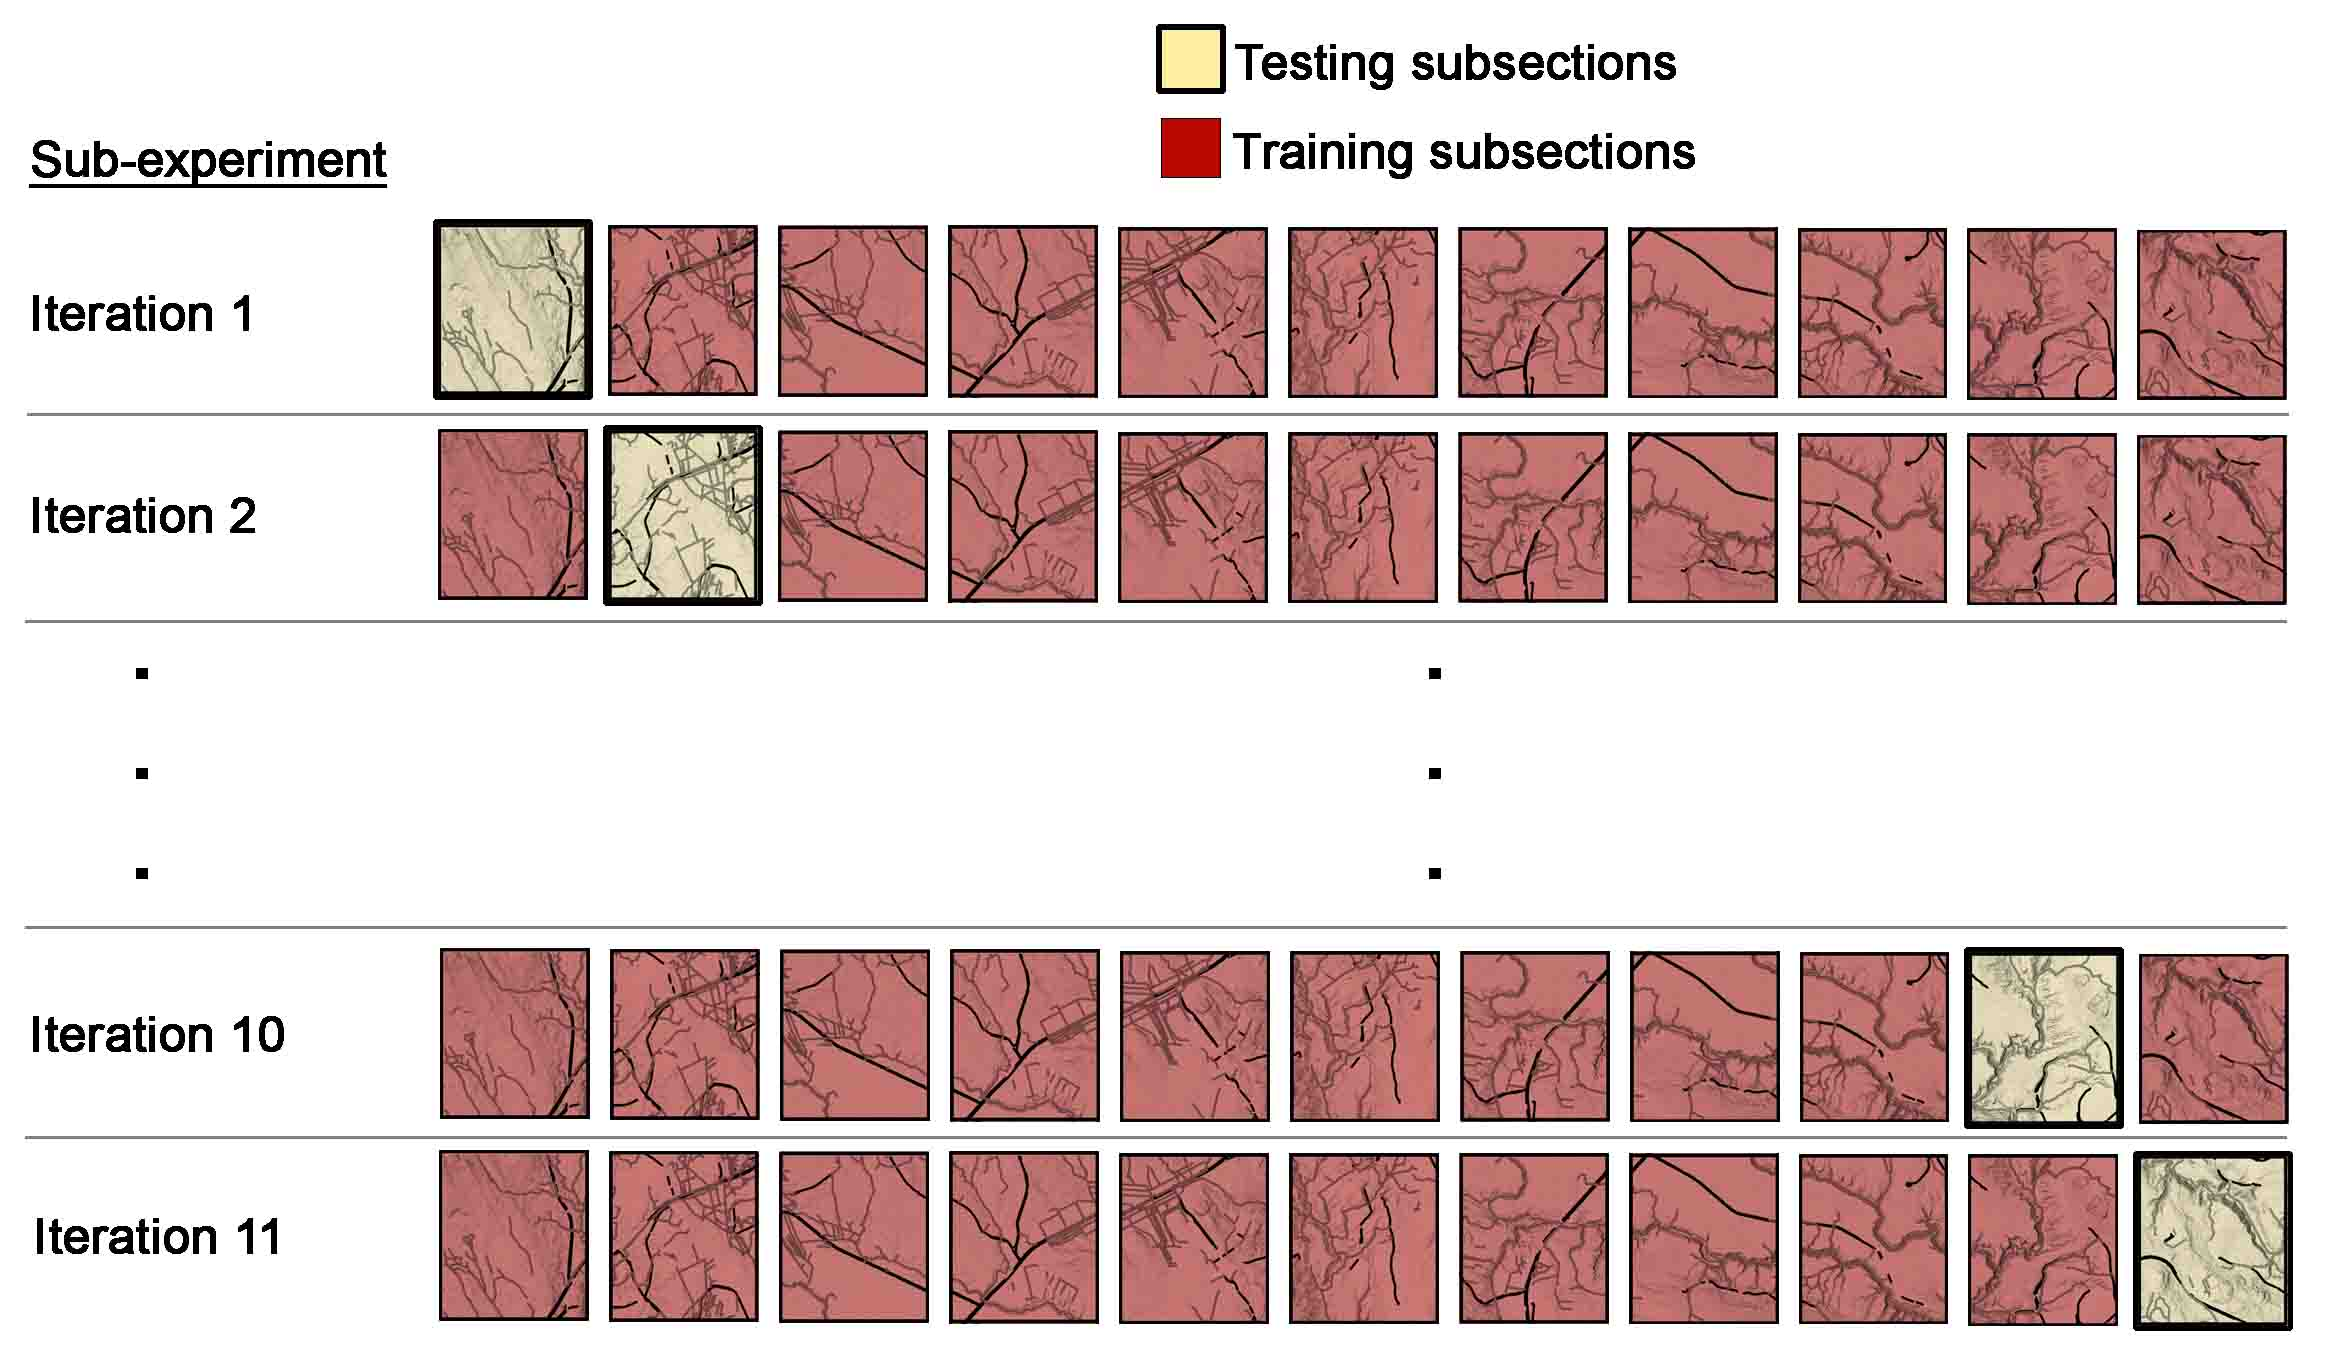
\includegraphics[width=1\linewidth]{images/cross_validation_lo.jpg}
    \caption{11-fold cross validation. Each subsection in the hold-out data was used once for testing, with the remaining subsections being used to build a new model for each iteration.}
    \label{fig:crossvalidation}
\end{figure}

\subsection{Developing the Random Forests model}

\textit{Model ensembles} is a category of machine learning where a set of models can be combined to increase diversity and robustness of predictions \citep{flach}. Random Forests is a supervised learning algorithm, first developed by \citet{breiman}, that makes use of the model ensemble technique by using a set of decision trees to build a \textit{forest} of trees. The outputs from these trees are then examined, and a class probability estimation ranging from 0 to 1 can be produced for each sample by dividing the amount of tree outputs of a class with the total amount of trees \citep{breiman}.

The decision tree data structure is a \textit{tree} of connected nodes where the end node of each branch (leaf) produces an output value. Each step in the tree aims to minimise the entropy of the outputs \citep{kotsiantis}. Each node in a decision tree represents a variable or an abstraction of variables from the inputs and each split is made by using this variable to separate the inputs.

Random Forests uses two techniques called \textit{subspace sampling} and \textit{bootstrap aggregation} (bagging) in tandem \citep{breiman}. Subspace sampling is the process of drawing a random subset of variables from the input variable set \citet{ho}. The bagging technique takes, with replacement, a set of different random samples for constructing each tree \citep{flach}. There are several hyperparameters that can be tuned to achieve better results from the model. For example, you can adjust the amount of decision trees to use, or the maximum amount of input variables to use for each subspace sampling \citep{scikit-learn}. We performed a hyperparameter tuning to determine what parameter values for the Random Forests algorithm would yield the best prediction. Using 300 trees and \textit{gini} as the splitting criterion, with a minimum of 10 samples per node split, and no artificial class weight or max depth of trees produced the best results.

Random Forests computes Gini importance, which shows how often a variable is selected for a split for a certain classification \citep{gini}. Each input variable is given a Gini impurity rating, which measures the frequency of incorrect labelling occurring from its use. As the Gini impurity rating for a variable increases, its Gini importance decreases \citep{gini}. When the model is trained, it examines the Gini importance from all trees and produces the total Gini importance as a value between 0 and 1 \citep{gini}. The Gini importance can help when developing a model by indirectly giving advice on new input variables to introduce.

The Random Forests algorithm from the Python library \textit{scikit-learn} was used in the experiment, and the classifiers were trained on all the input variables seen in \hyperref[featuretable]{Table} \ref{featuretable}. The probability predictions used in this Random Forests implementation are computed by counting the number of occurrences of a class output and dividing with the total amount of trees in the forest \citep{scikit-learn}. The testing phase showed that the classifiers produced poor results when the ratio of ditch- versus non-ditch pixels in the training data was very high. A high ratio led to the models not being punished for mislabelling ditches as non-ditches, causing it to prioritise a high accuracy over a high recall. According to \citet{balanced}, an imbalanced training dataset causes a minority class to be less accurately predicted. Because the ditch class is much less common than the non-ditch class, we attempted to train the models with a roughly equal amount of ditch pixels and non-ditch pixels to balance the models. The models were, however, still evaluated on all the pixels in the 11 validation subsections.

\begin{table} [!htb]
    \tbl{The 40 input variables used when training the models.}
    {\begin{tabular}{ll} \toprule
      Variable/Algorithm\textsuperscript{a} & Circular radii\textsuperscript{b} \\ \midrule
      
      Sky View Factor median &2, 6 \\
      Sky View Factor standard deviation & 6 \\
      Sky View Factor min & 6 \\
      Sky View Factor max & 2, 4, 6 \\
      Sky View Factor non ditch amplification & - \\ 
      Sky View Factor Gabor & - \\
      Sky View Factor Gabor - streams removed & -\\
      
      Impoundment mean & 2, 3, 4, 6 \\
      Impoundment median & 2, 4, 6 \\
      Impoundment standard deviation & 4, 6 \\
      Impoundment max & 6 \\
      Impoundment ditch amplification & - \\
      Impoundment ditch amplification - streams removed & - \\
      
      HPMF mean & 3, 4, 6 \\
      HPMF median & 4 \\
      HPMF standard deviation & 6 \\
      HPMF min & 2, 4 \\
      HPMF ditch amplification & - \\
      HPMF ditch amplification - streams removed & - \\
      HPMF Gabor - streams removed & -\\
      
      Slope mean & 6 \\
      Slope median & 6 \\
      Slope standard deviation & 4, 6 \\
      Slope min & 2, 4, 6 \\
      %Slope max & 2, 4, 6 \\
      Slope non-ditch amplification & - \\ \bottomrule
    \end{tabular}}
    \tabnote{\textsuperscript{a} Displays algorithm used to produce the variable. \newline
        \textsuperscript{b} Represents the radius of the circular mask (if one was used) to determine \newline what neighbouring pixels to use in an algorithm. The radii represents pixels \newline \mbox{with a 0.5 m resolution.\itshape\ignorespaces}}
    \label{featuretable}
\end{table}

The first step to create a more balanced training dataset was to extract all pixels labelled as ditches, as well as pixels within close proximity of ditches. Secondly, pixels were sampled randomly from the entire subsection. This allowed the training dataset to be fairly balanced while still containing most of the geographical features of each subsection (\hyperref[fig:balancedmasks]{Figure} \ref{fig:balancedmasks}).

\begin{figure} [!htb]
    \centering
    \subfigure[]{
        \resizebox*{6.85cm}{!}{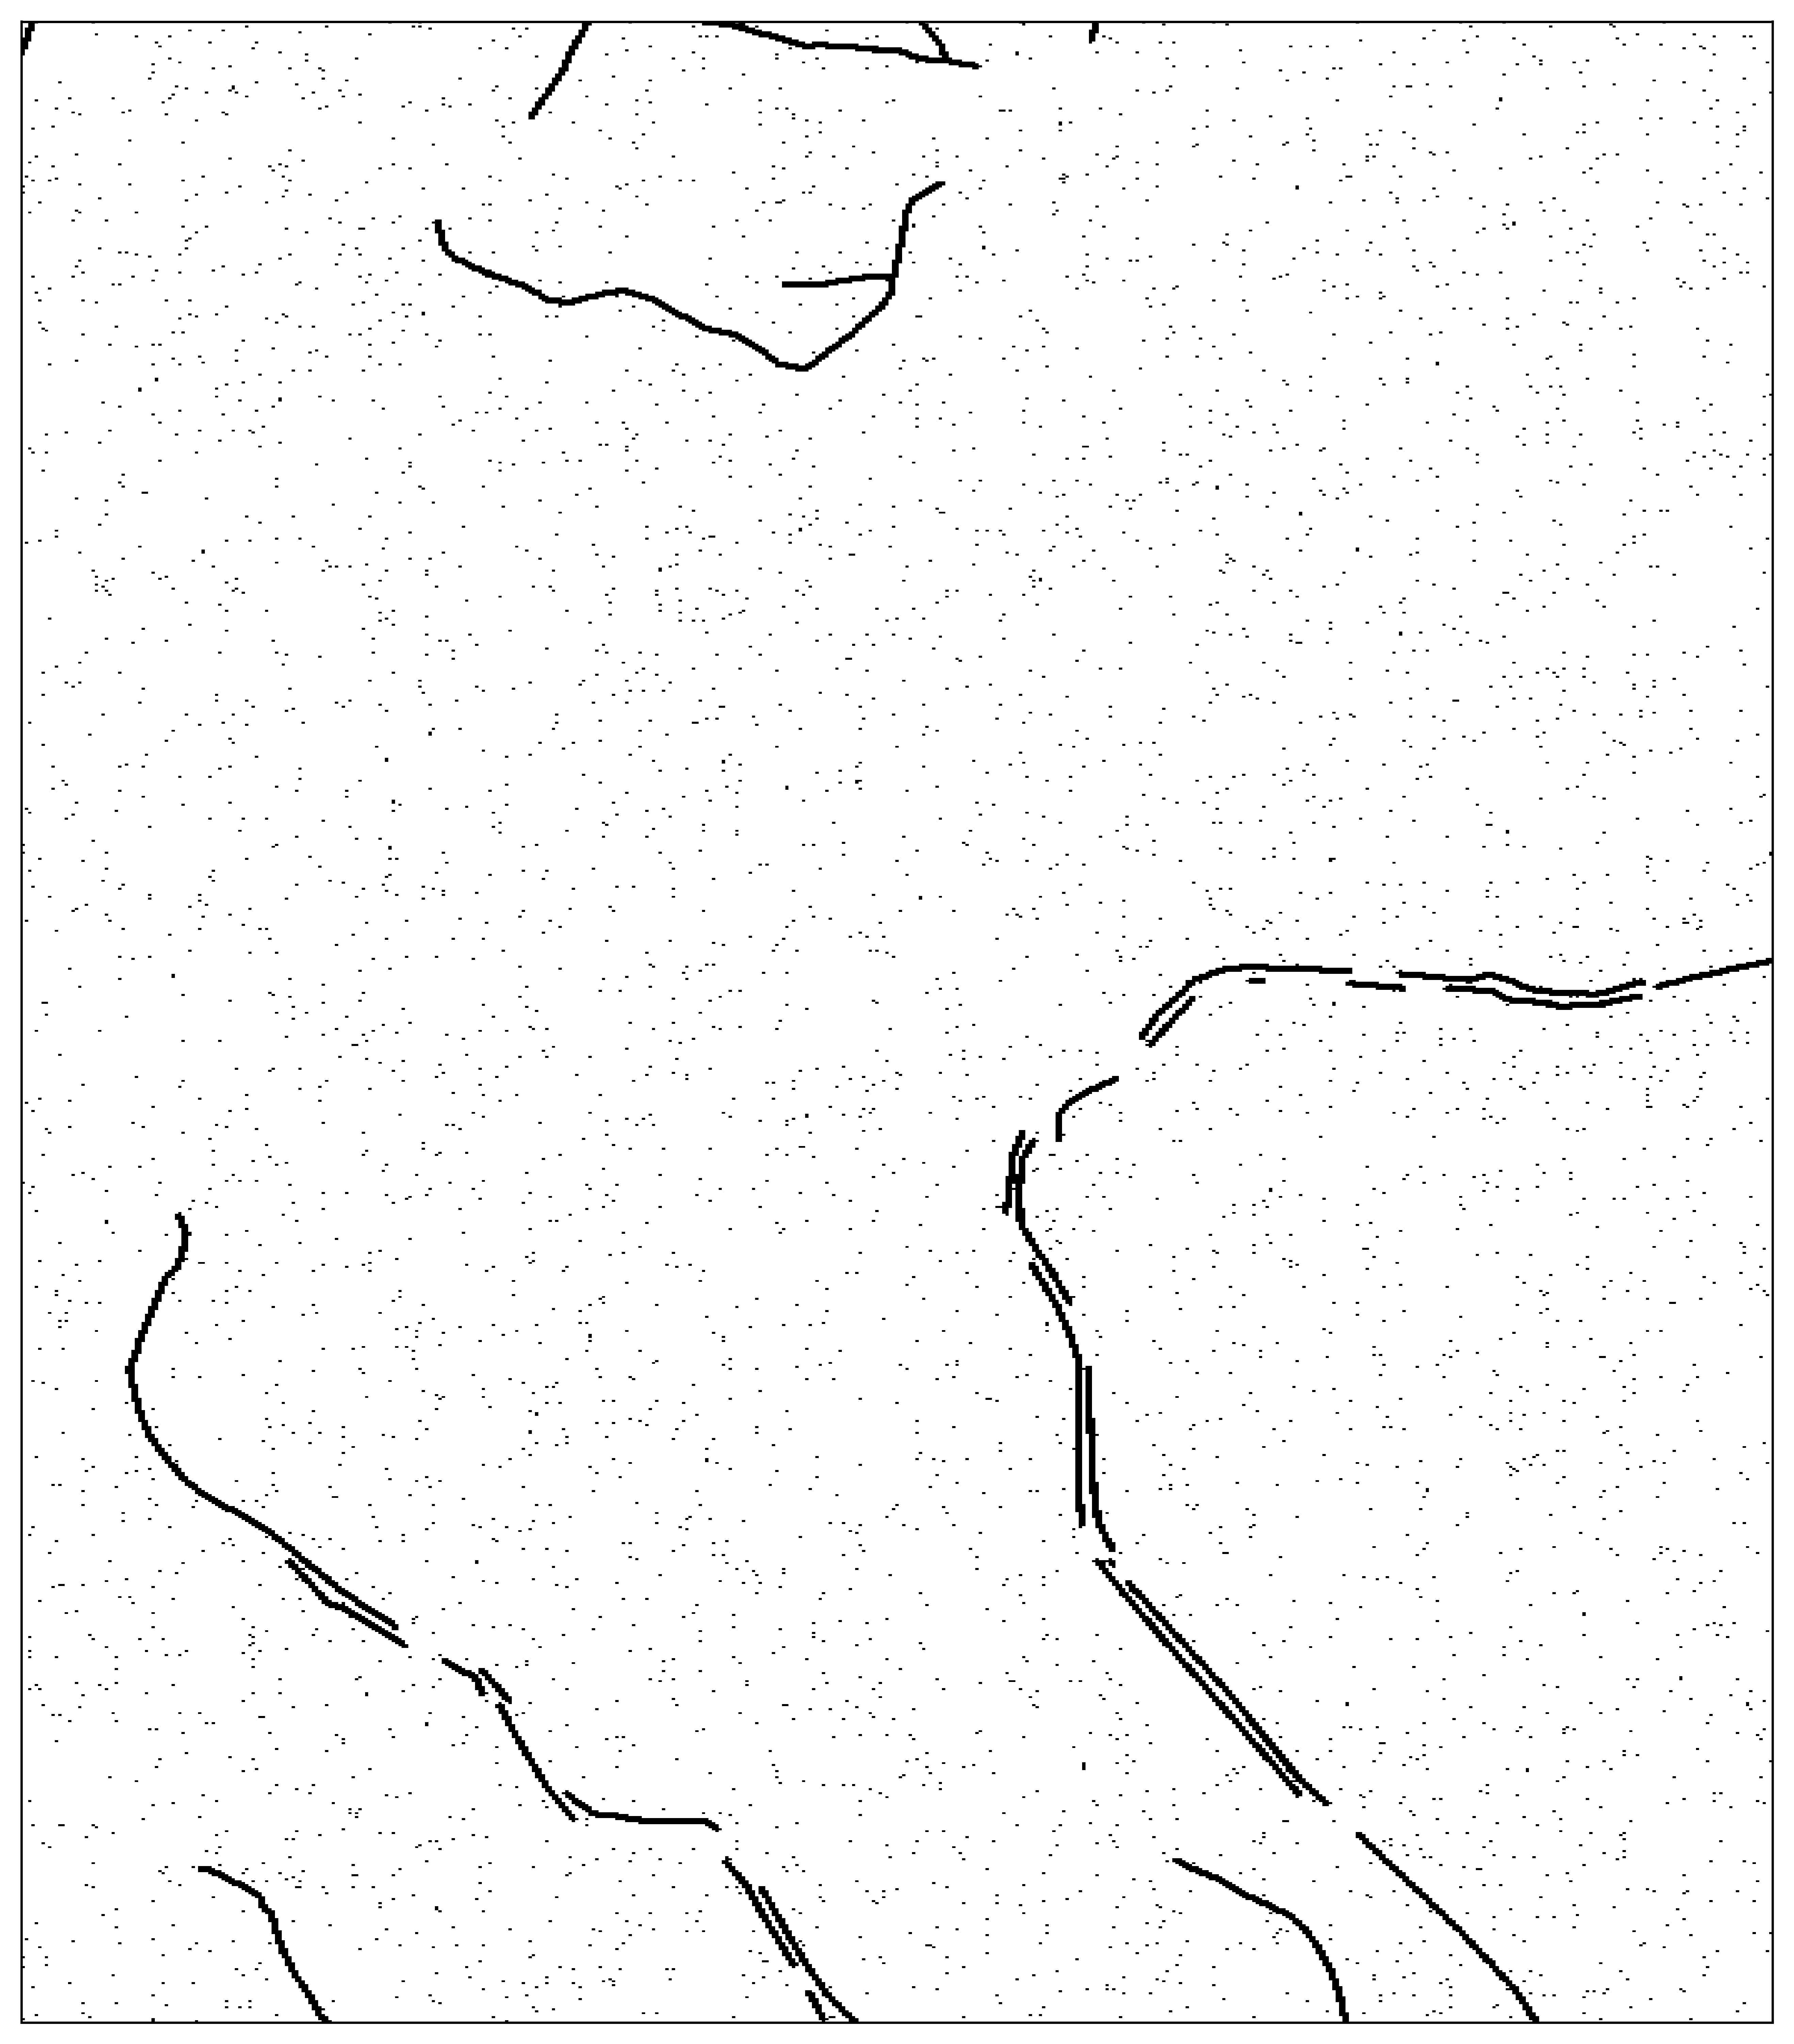
\includegraphics{./images/publ_balanced_masks_A_lo.jpg}}}\hspace{5pt}
    \subfigure[]{
        \resizebox*{6.85cm}{!}{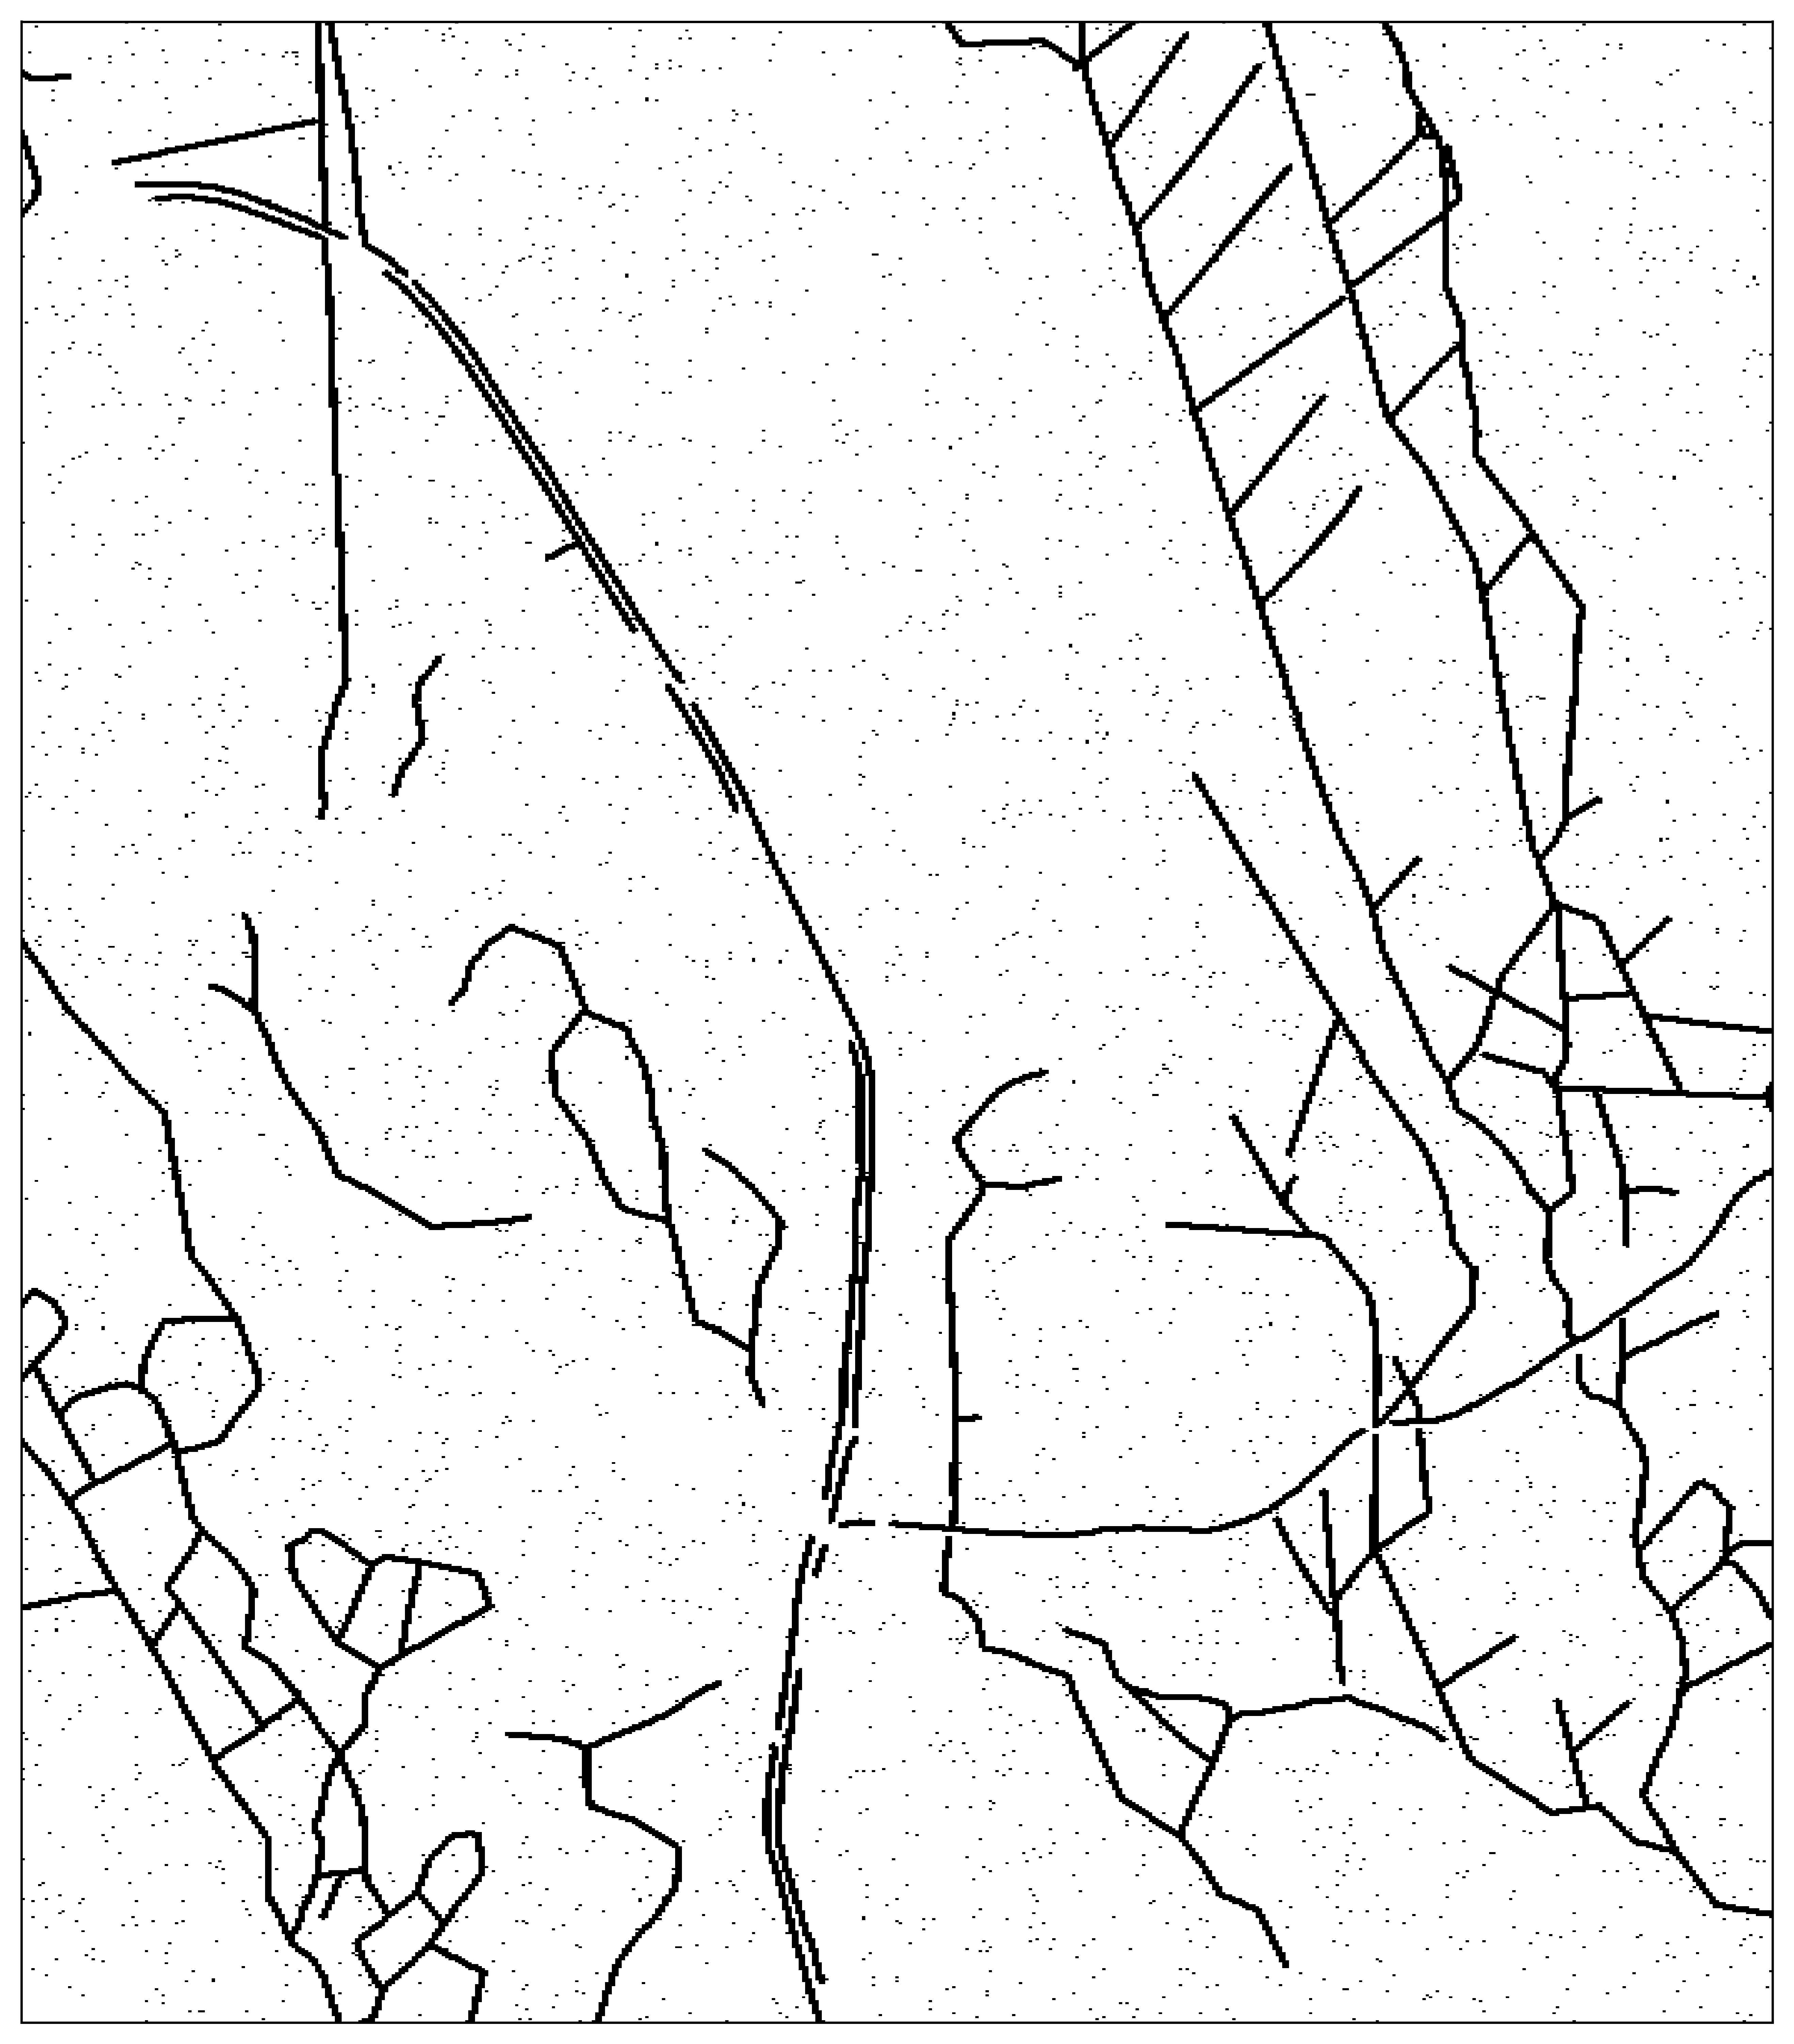
\includegraphics{./images/publ_balanced_masks_B_lo.jpg}}}
    \caption{Black pixels here indicate the balanced masks used to determine what pixels were used when training the models. \textbf{a, b: }Examples of two subsection from the training dataset.}
    \label{fig:balancedmasks}
\end{figure}

\subsection{Post-processing}
The models output a ditch class probability prediction for each pixel. Values close to zero indicate a low probability of a pixel lying in a ditch, whereas values close to one equals a high ditch probability (\hyperref[fig:postprocessing1]{Figure} \ref{fig:postprocessing1} \hyperref[fig:postprocessing1]{a}).

\subsubsection{Noise reduction and gap filling}
The probability predictions contained a lot of noise in  the areas largely distant from the ditches. The first step for removing this noise was to use a bilateral de-noising filter on the entire prediction image. This left linear properties and pixels with a very high value intact, while lowering the value of pixels that did not contribute to an accurate prediction (\hyperref[fig:postprocessing1]{Figure} \ref{fig:postprocessing1} \hyperref[fig:postprocessing1]{b}).

\begin{figure} [!htb]
    \centering
    \subfigure[]{
        \resizebox*{6.85cm}{!}{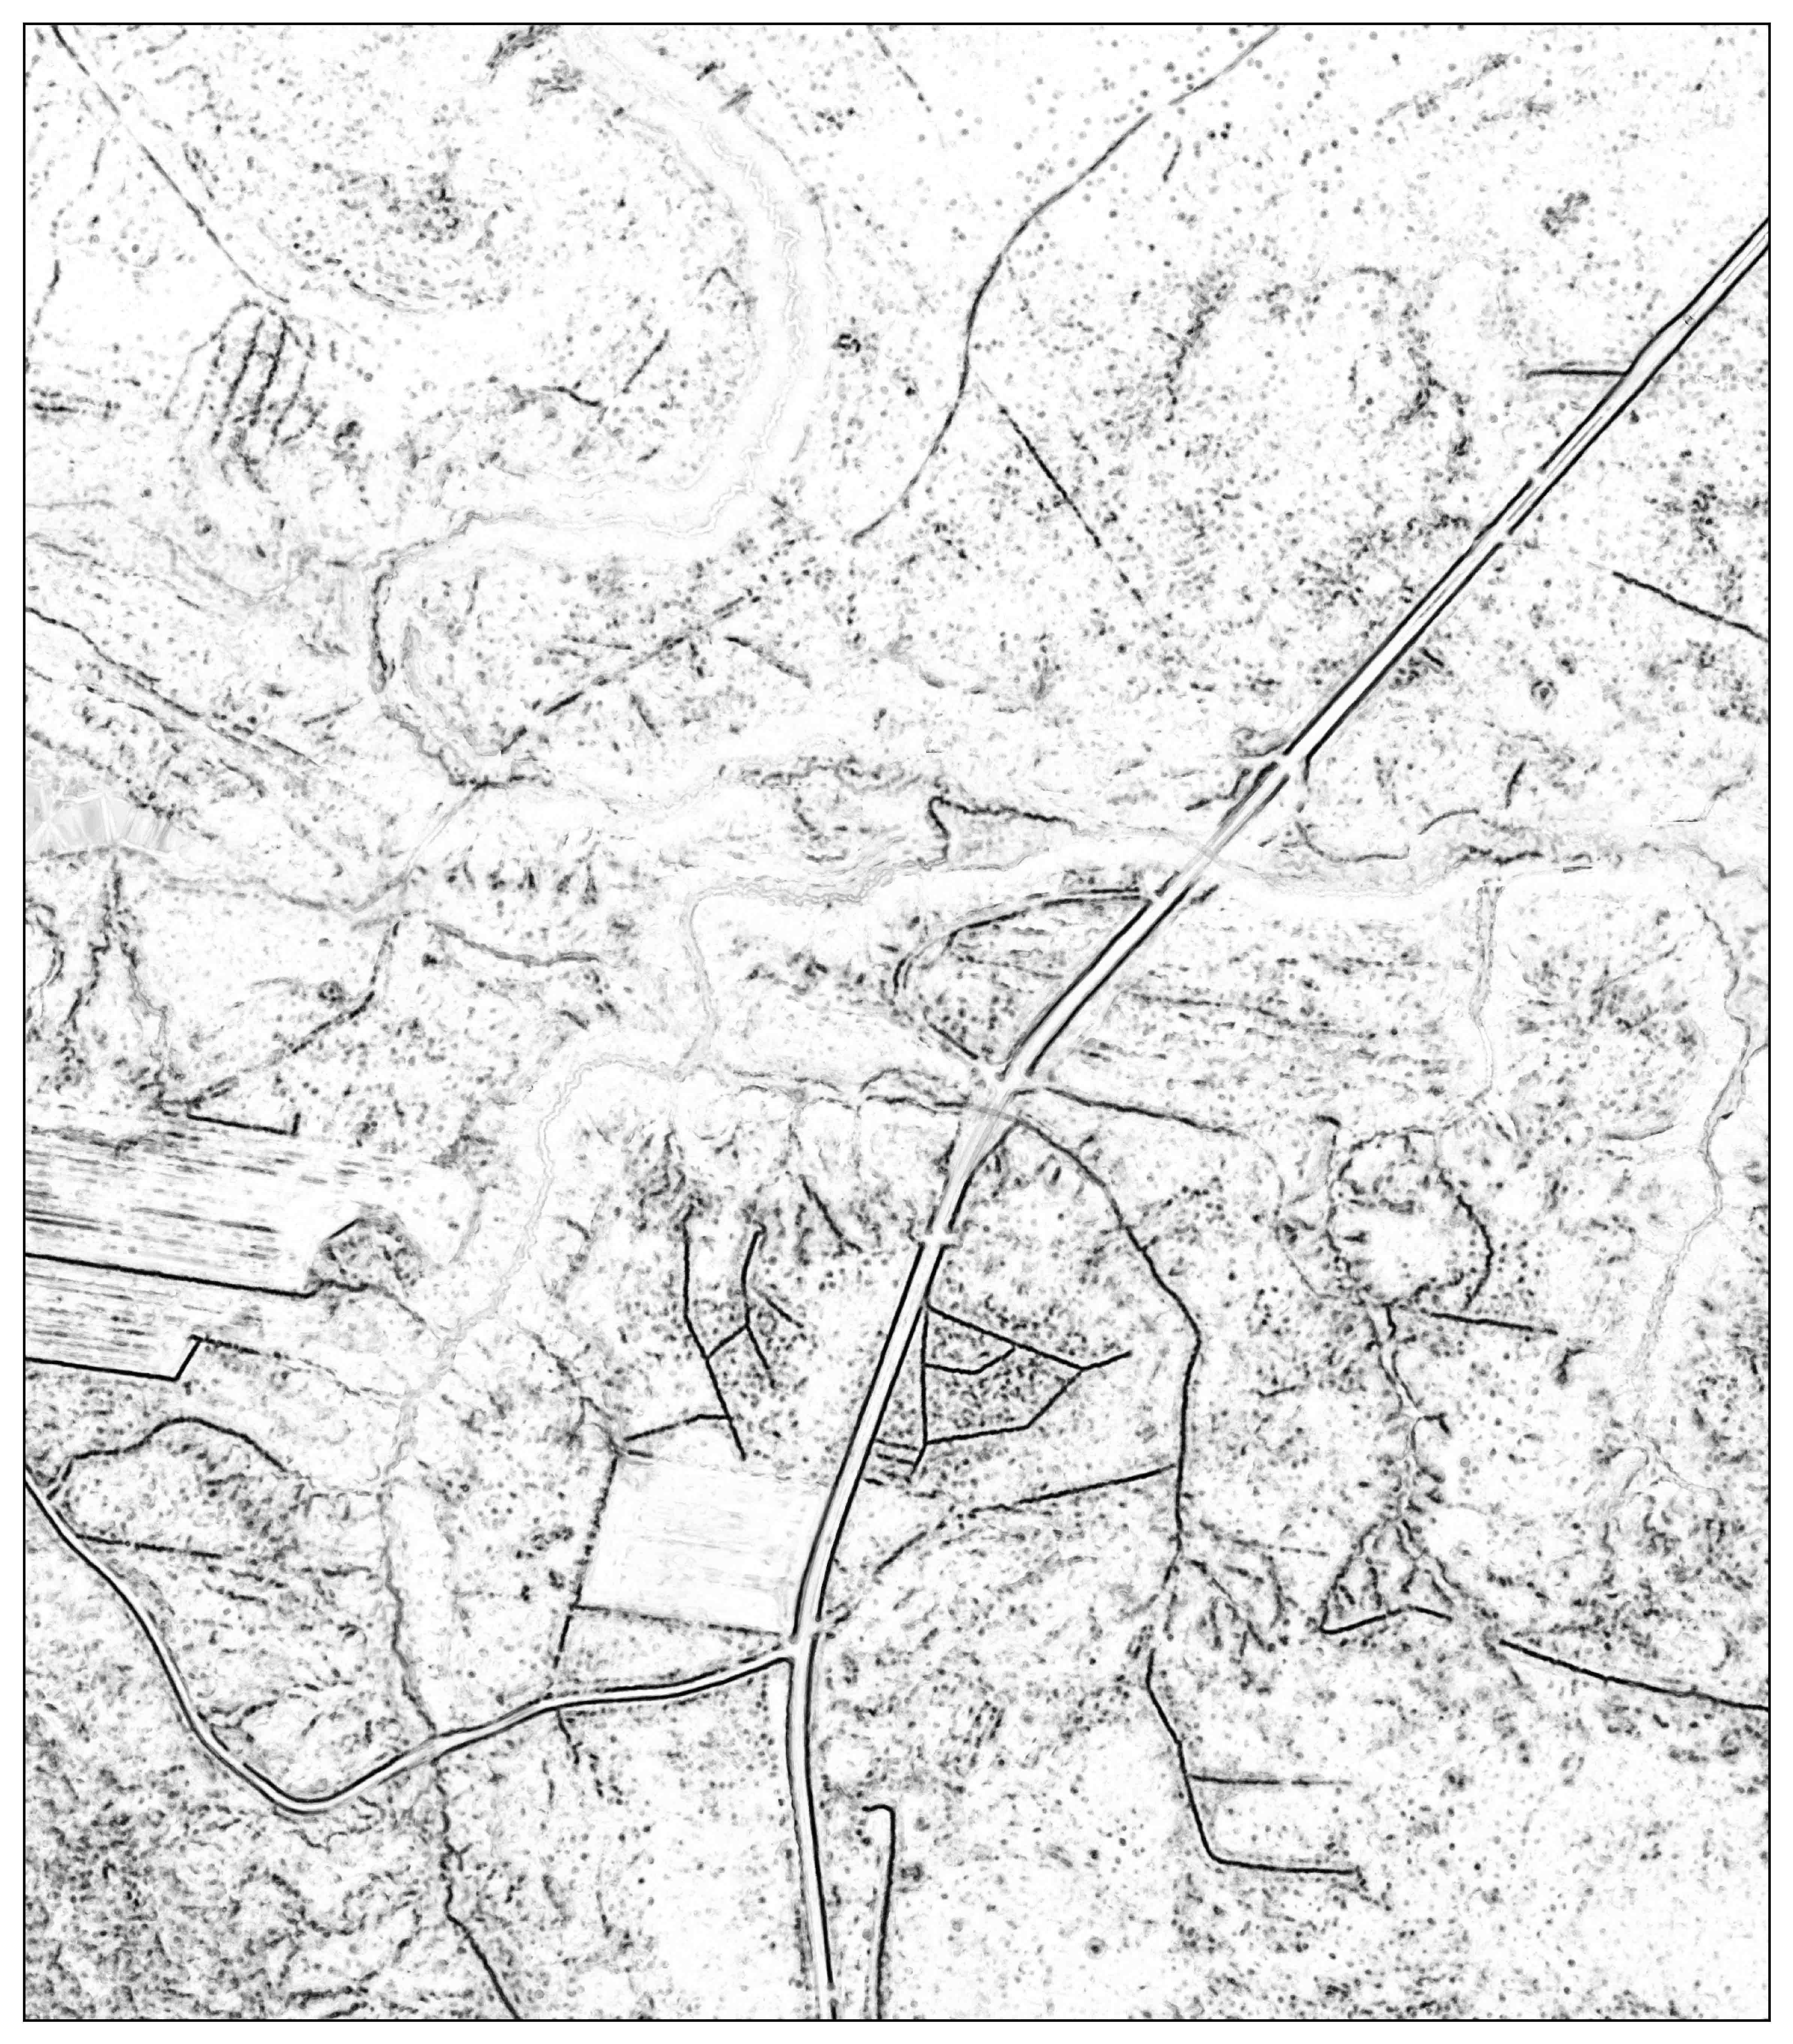
\includegraphics{./images/publ_post_process_step_1_lo.jpg}}}\hspace{5pt}
    \subfigure[]{
        \resizebox*{6.85cm}{!}{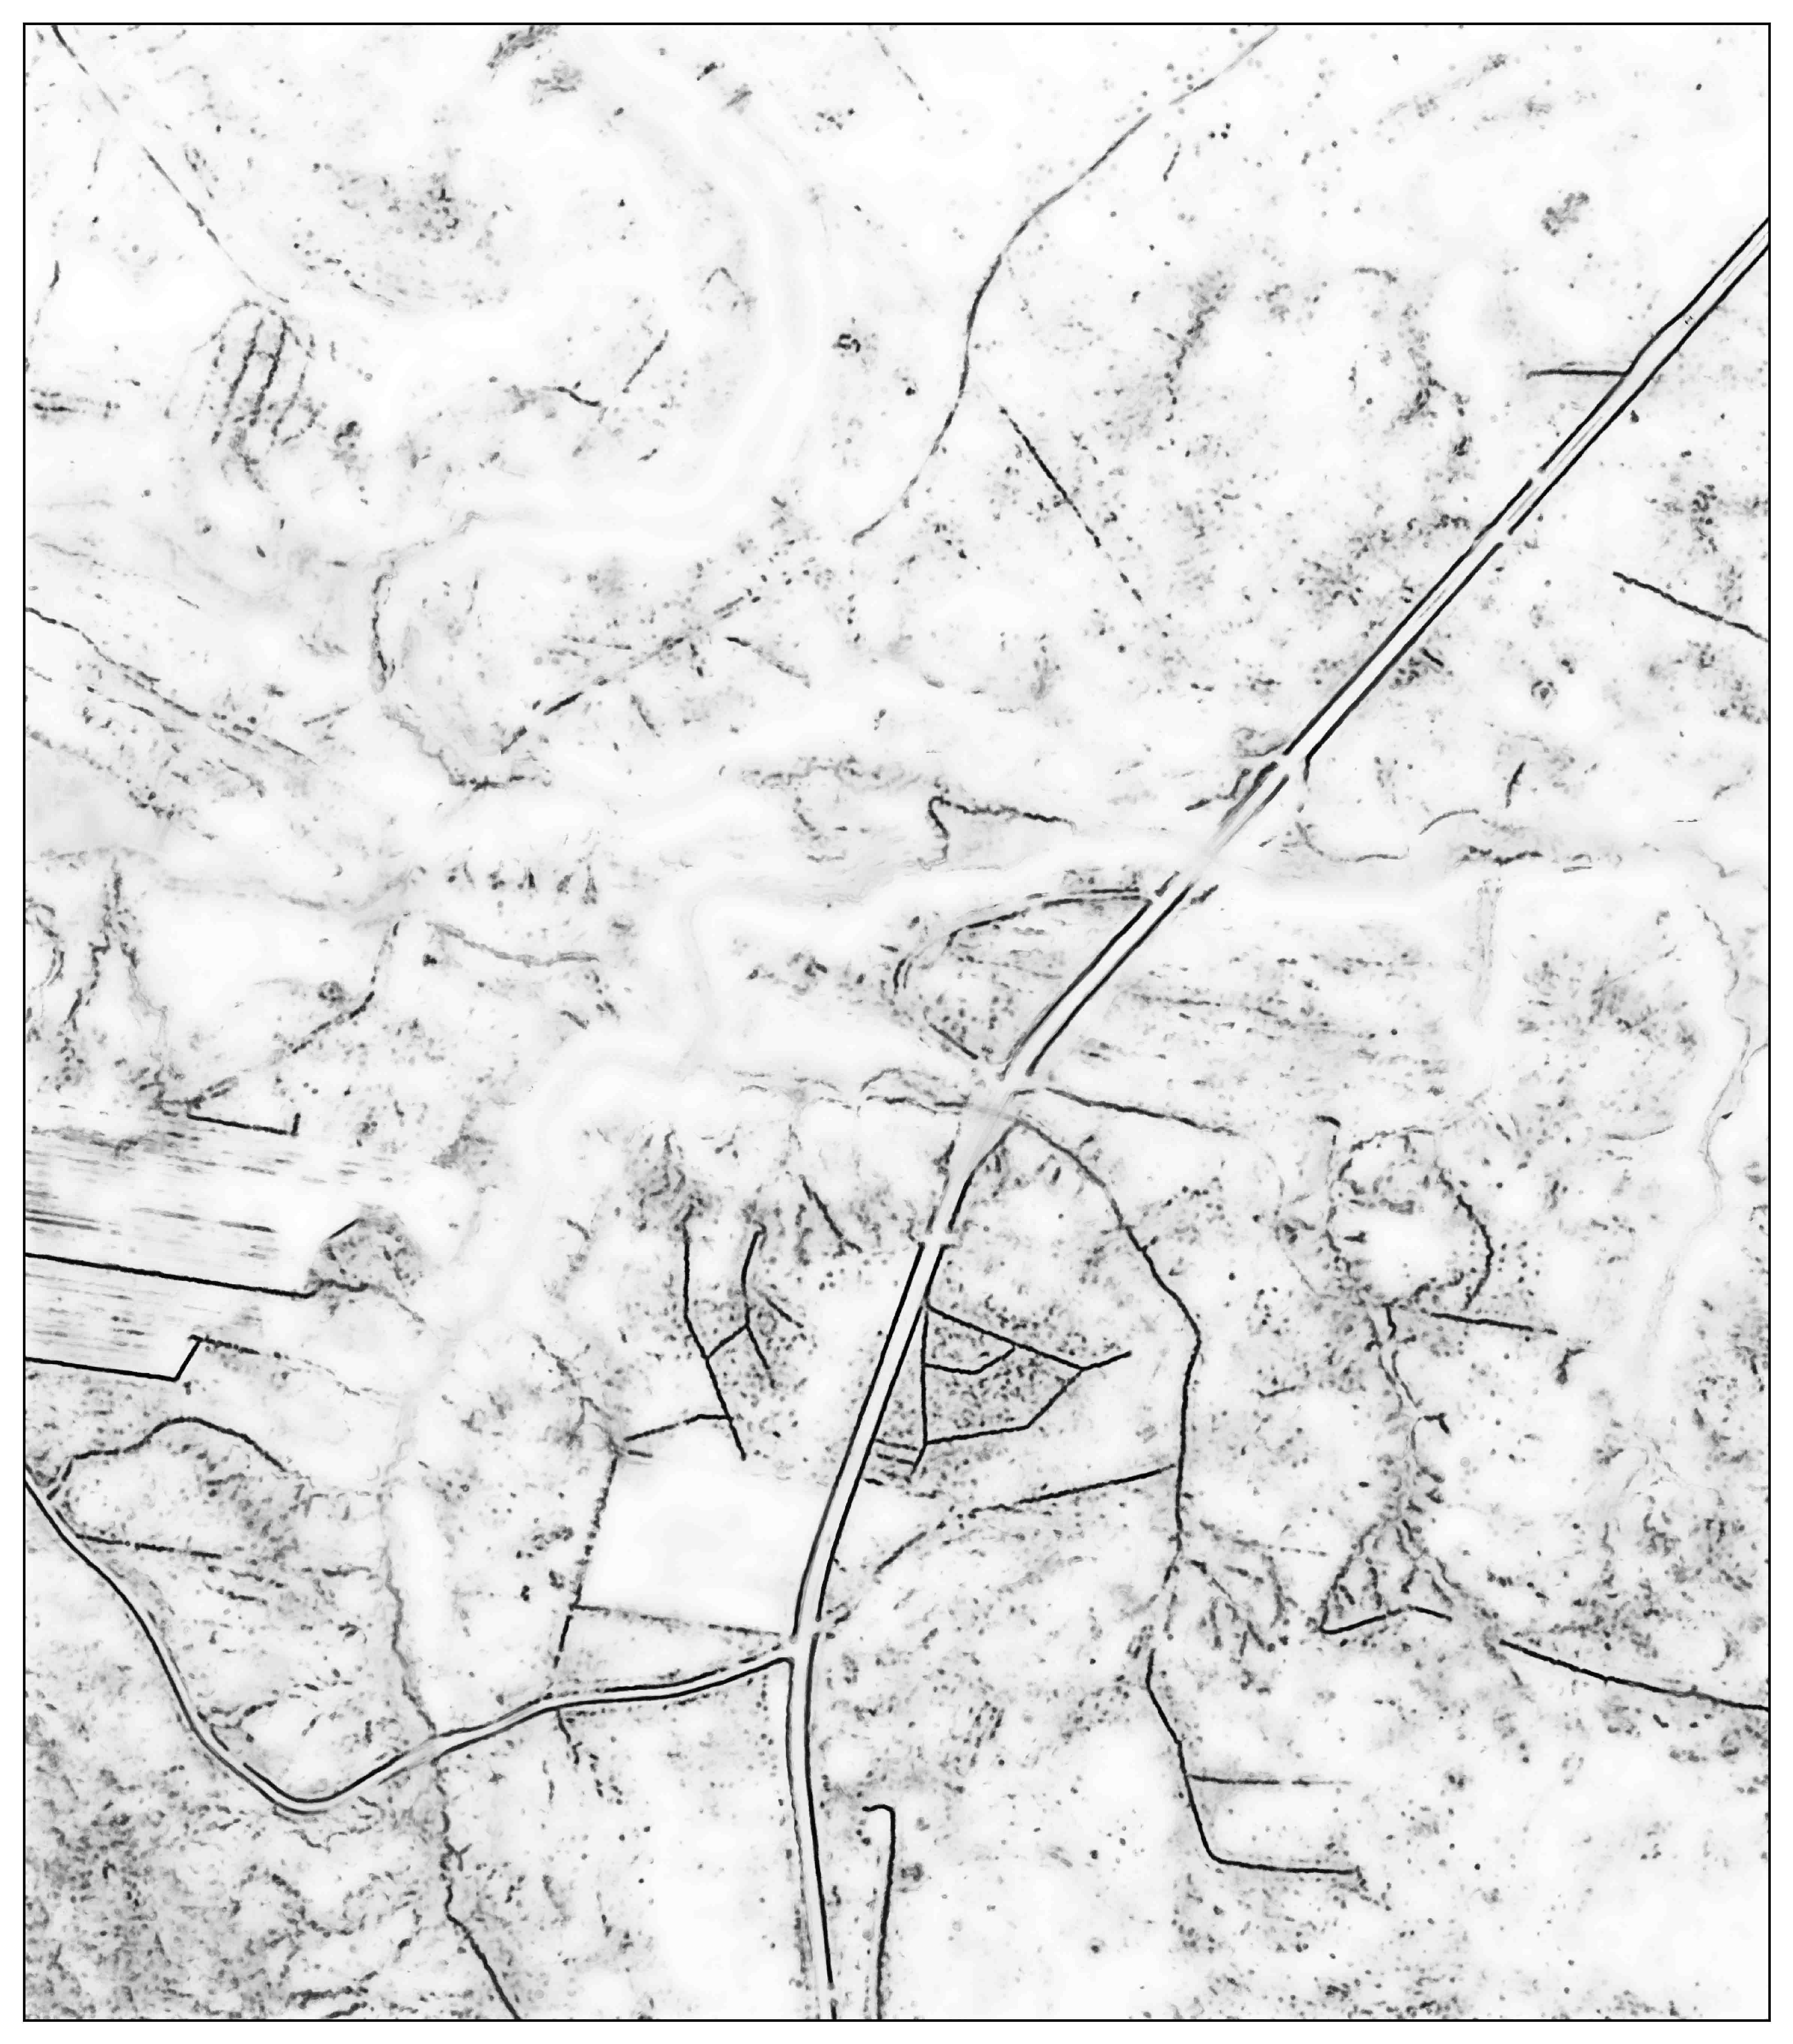
\includegraphics{./images/publ_post_process_step_2_lo.jpg}}}
    \caption{Step one and two of the post-process. Darker pixels indicate a higher ditch probability. \textbf{a: }Random Forests probability prediction. \textbf{b: }Bilateral de-noising.}
    \label{fig:postprocessing1}
\end{figure}

The second step for removing noise was to use a custom function to remove pixels that had a semi-high ditch probability, but that lay far away from any other high probability pixels. In this function, a threshold value was used to avoid removing pixels with a high enough ditch probability, helping to retain pixels that lay in or close to a ditch. The maximum ditch probability value in a circular radius of 10 pixels was then calculated. If this maximum value was too low, the probability value of the examined pixel was lowered (\hyperref[fig:postprocessing2]{Figure} \ref{fig:postprocessing2} \hyperref[fig:postprocessing2]{a}).

The third step involved taking measures to try to fill gaps in ditches that the models failed to correctly predict. This was done by aggregating pixels covered by cone masks expanding outwards in different directions from the examined pixel. This step also amplified some of the noise that was left, but filling the gaps in the ditches was judged to be more important to help make the next step more effective (\hyperref[fig:postprocessing2]{Figure} \ref{fig:postprocessing2} \hyperref[fig:postprocessing2]{b}).

\begin{figure} [!htb]
    \centering
    \subfigure[]{
        \resizebox*{6.85cm}{!}{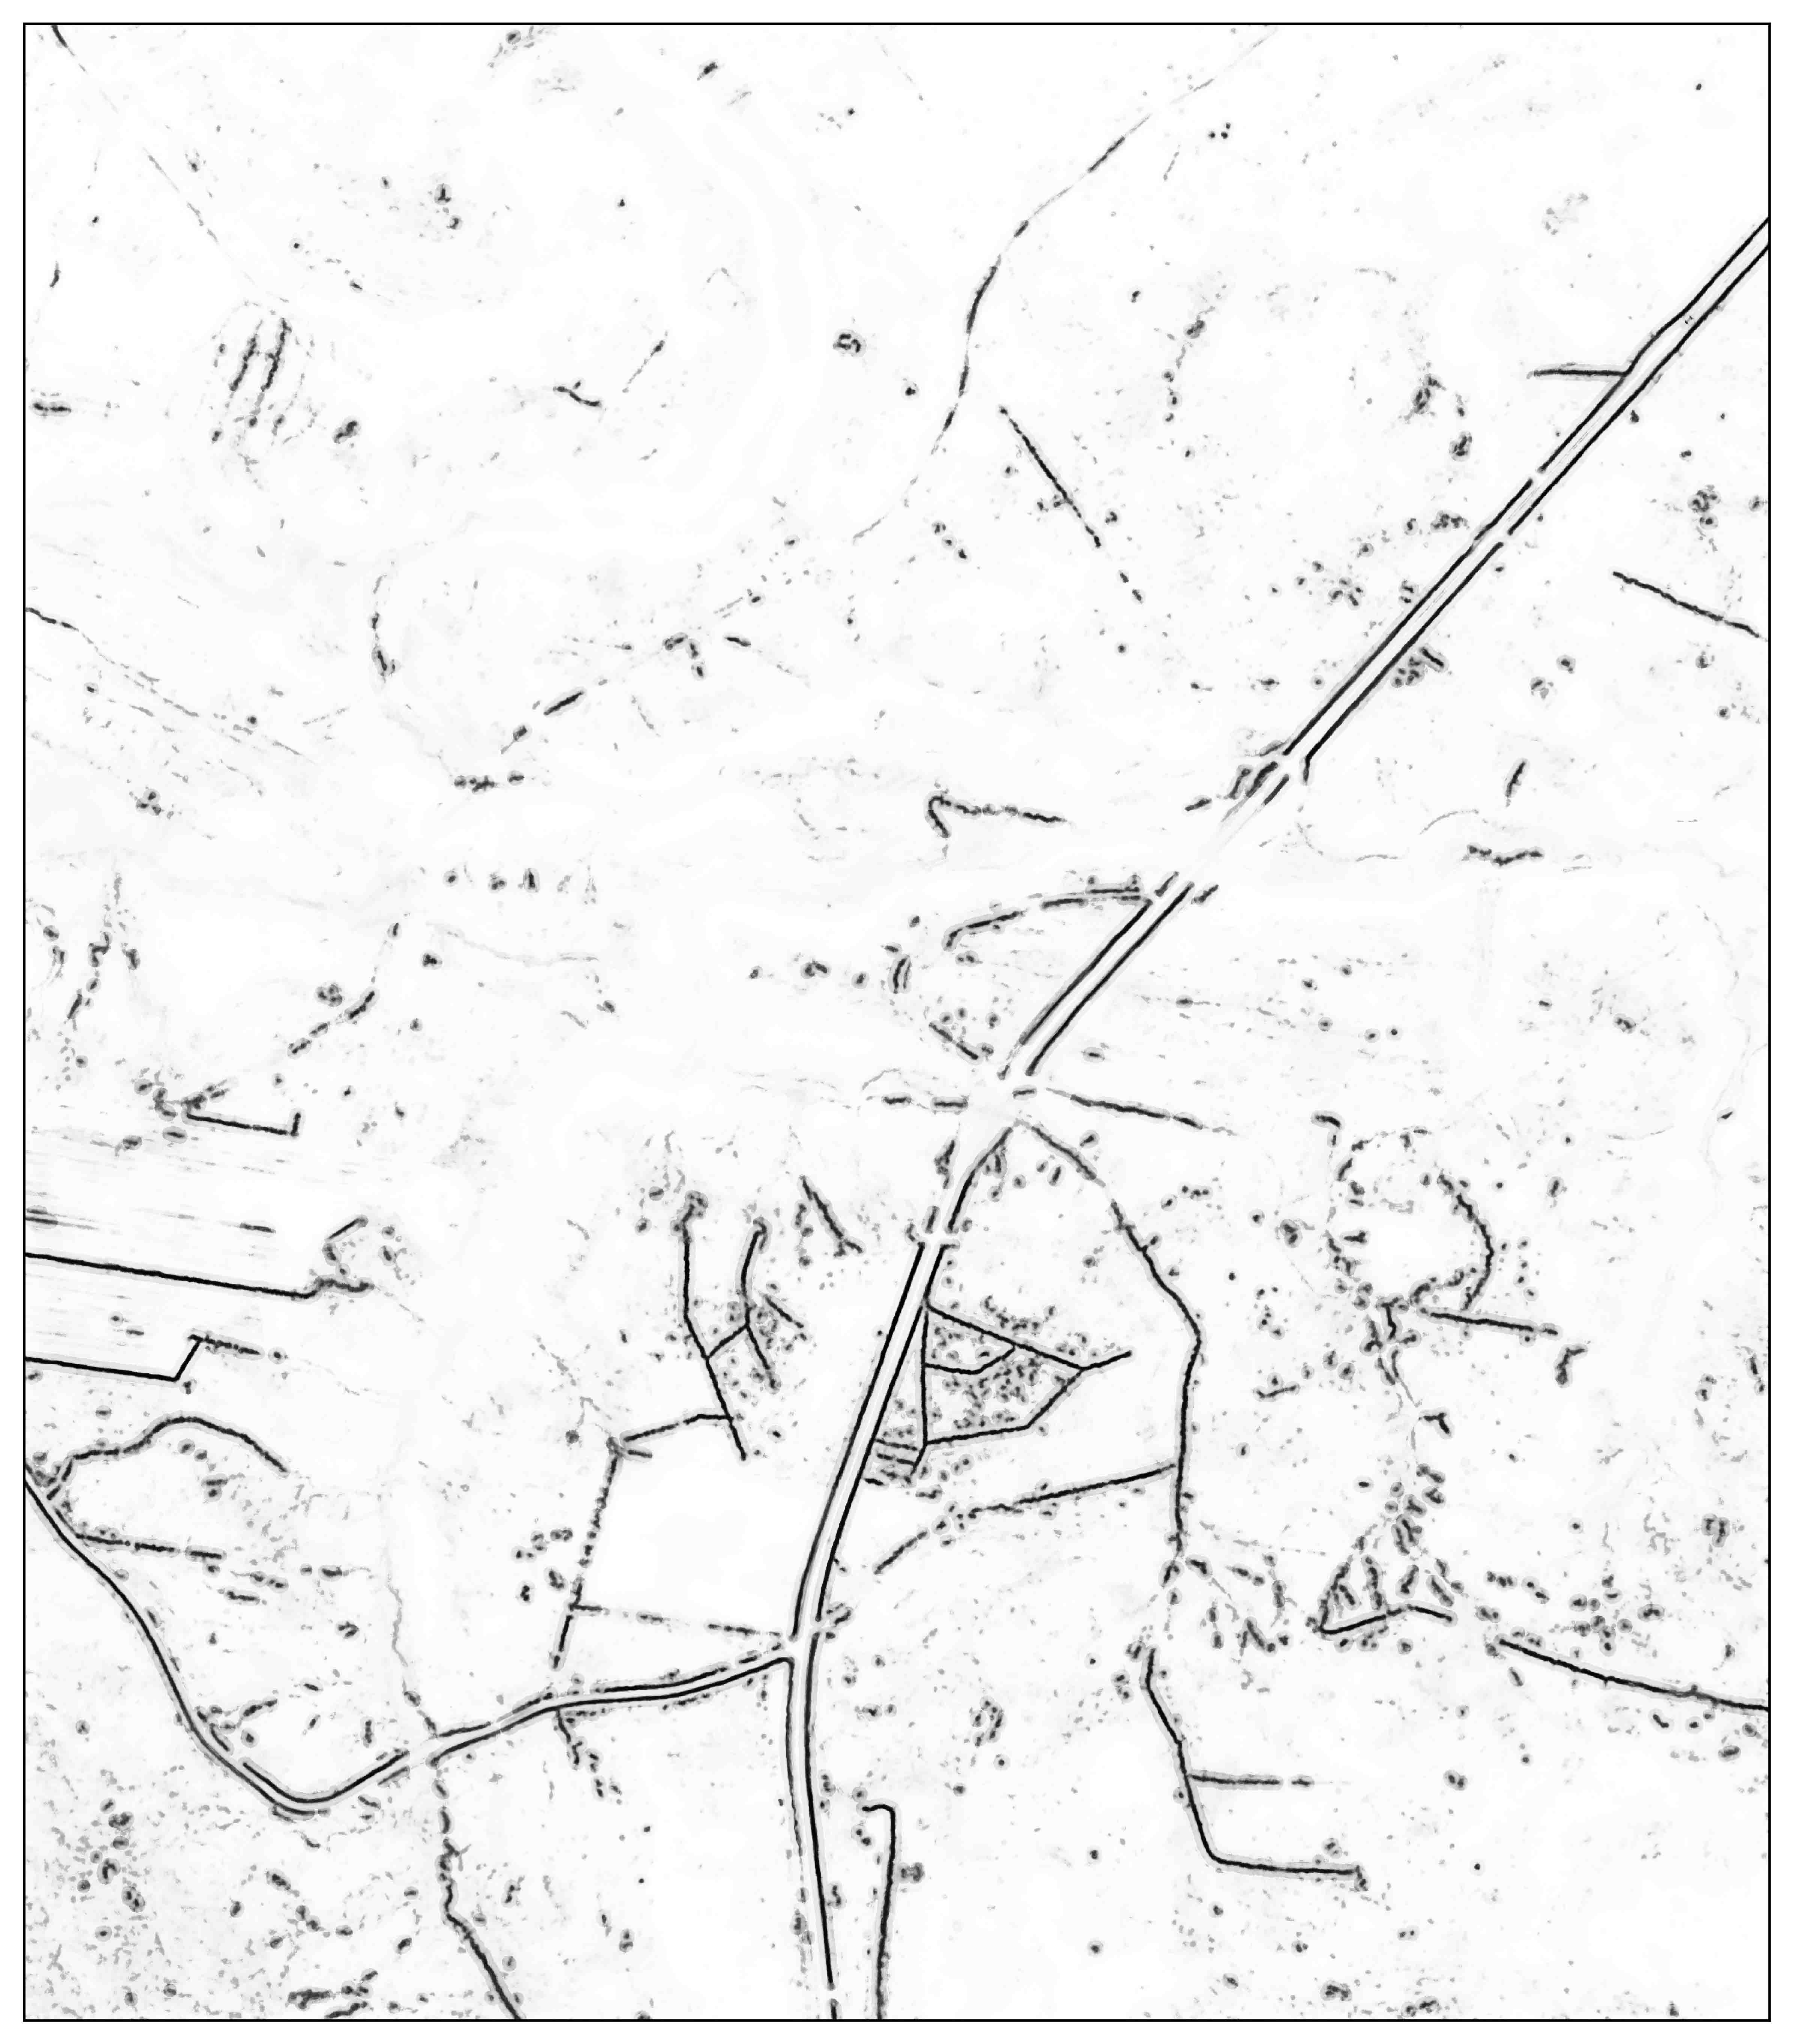
\includegraphics{./images/publ_post_process_step_3_lo.jpg}}}\hspace{5pt}
    \subfigure[]{
        \resizebox*{6.85cm}{!}{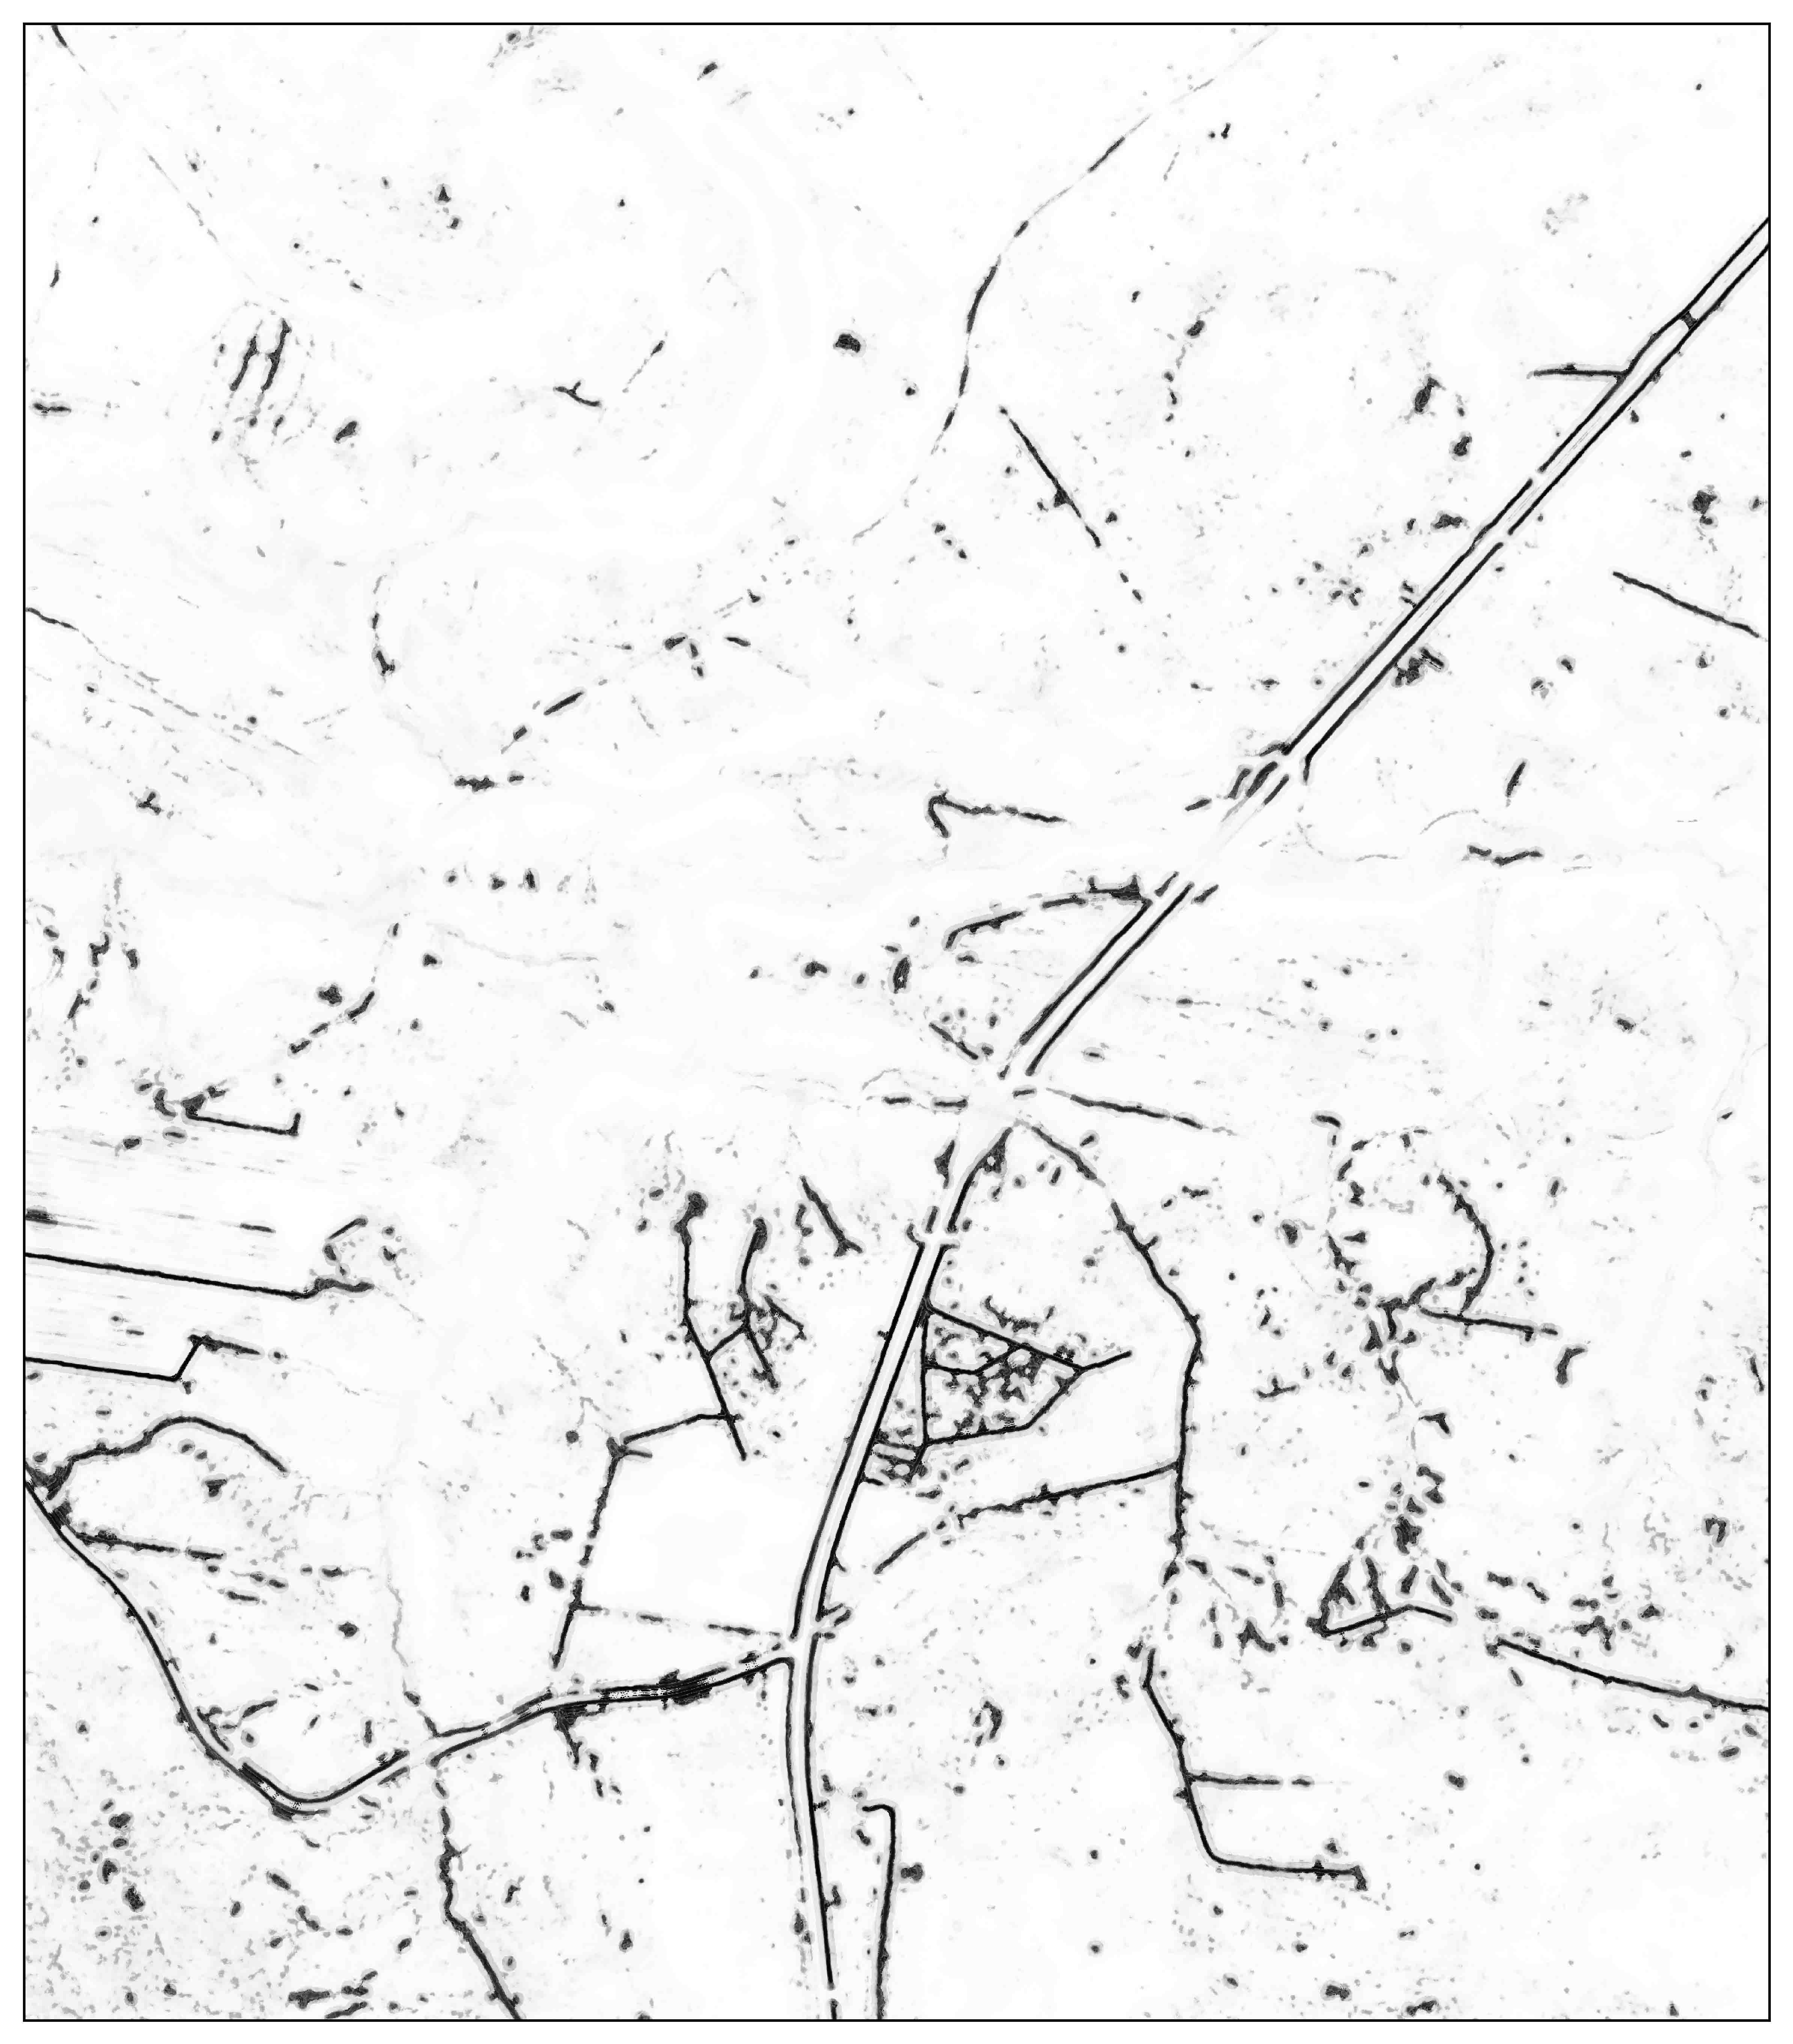
\includegraphics{./images/publ_post_process_step_4_lo.jpg}}}
    \caption{Step three and four of the post-process. Darker pixels indicate a higher ditch probability. \textbf{a: }Custom de-noising. \textbf{b: }Gap filling.}
    \label{fig:postprocessing2}
\end{figure}

\subsubsection{Binarisation with grid zones}
The models' ditch prediction is given in the original resolution raster format. To allow for comparison to the evaluation data, the same grid conversion was performed on the prediction raster as on the evaluation data displayed in \hyperref[fig:ditchpreprocess]{Figure} \ref{fig:ditchpreprocess} \hyperref[fig:ditchpreprocess]{c}. After testing different combinations of zone sizes and probability values, a mean probability rating was calculated for each $6*6$ grid zone, classifying the entire zone as part of a ditch if the mean probability exceeded 40 \%. This zone partitioning helped to fill in gaps where lone pixels in ditches had been incorrectly classified. (\hyperref[fig:postprocessing3]{Figure} \ref{fig:postprocessing3} \hyperref[fig:postprocessing3]{a}).

\subsubsection{Cluster removal}
To remove noise from the binary prediction, a custom cluster detection algorithm was used. By finding the number of connected pixels with a true value and removing those whose cluster size were below a given threshold, minor noise in the prediction could be removed while still retaining most of the ditch pixels. Actual ditches that have a low probability and therefore create small clusters may still be excluded by this method, but the noise removal advantages were judged to outweigh the loss in recall. A distance calculation was also performed in tandem with this method to find the largest distance of pixels inside each given cluster. This helped to remove sinks and hollows that were not removed by the initial small cluster removal, but that did not have a linear directional characteristic, indicating that they did not represent a ditch (\hyperref[fig:postprocessing3]{Figure} \ref{fig:postprocessing3} \hyperref[fig:postprocessing3]{b}).

\begin{figure} [!htb]
    \centering
    \subfigure[]{
        \resizebox*{6.85cm}{!}{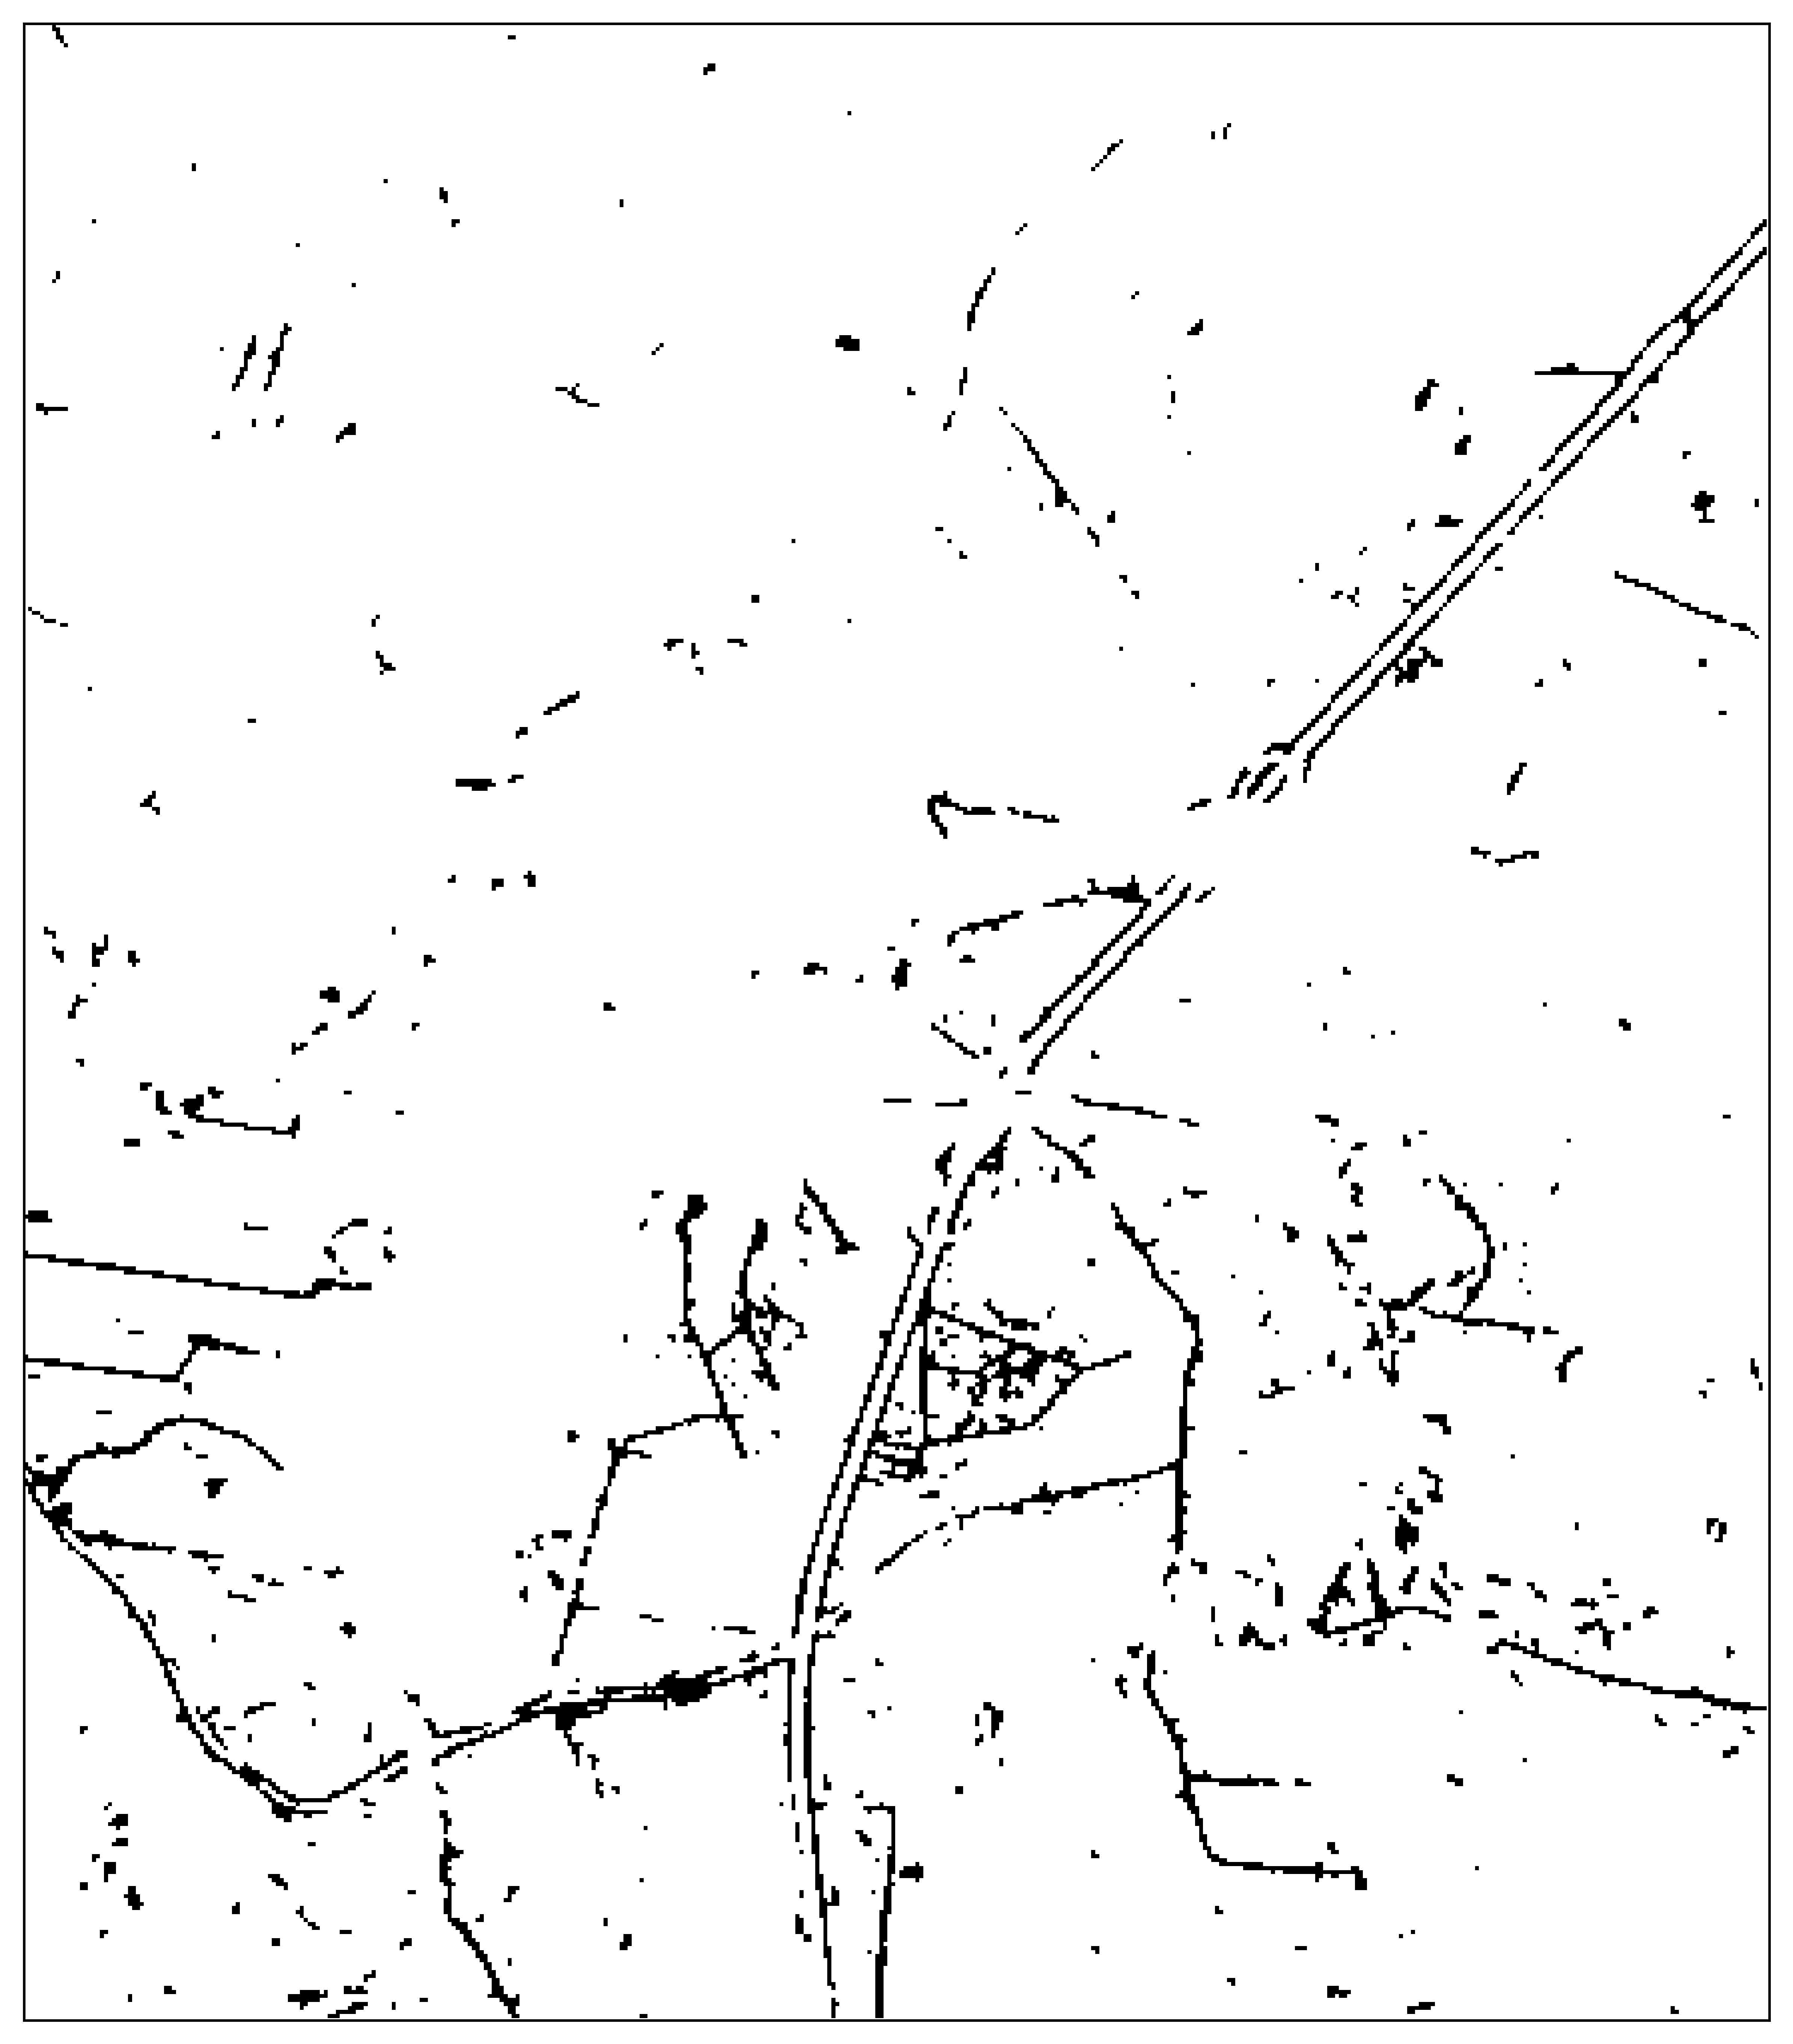
\includegraphics{./images/publ_post_process_step_5_lo.jpg}}}\hspace{5pt}
    \subfigure[]{
        \resizebox*{6.85cm}{!}{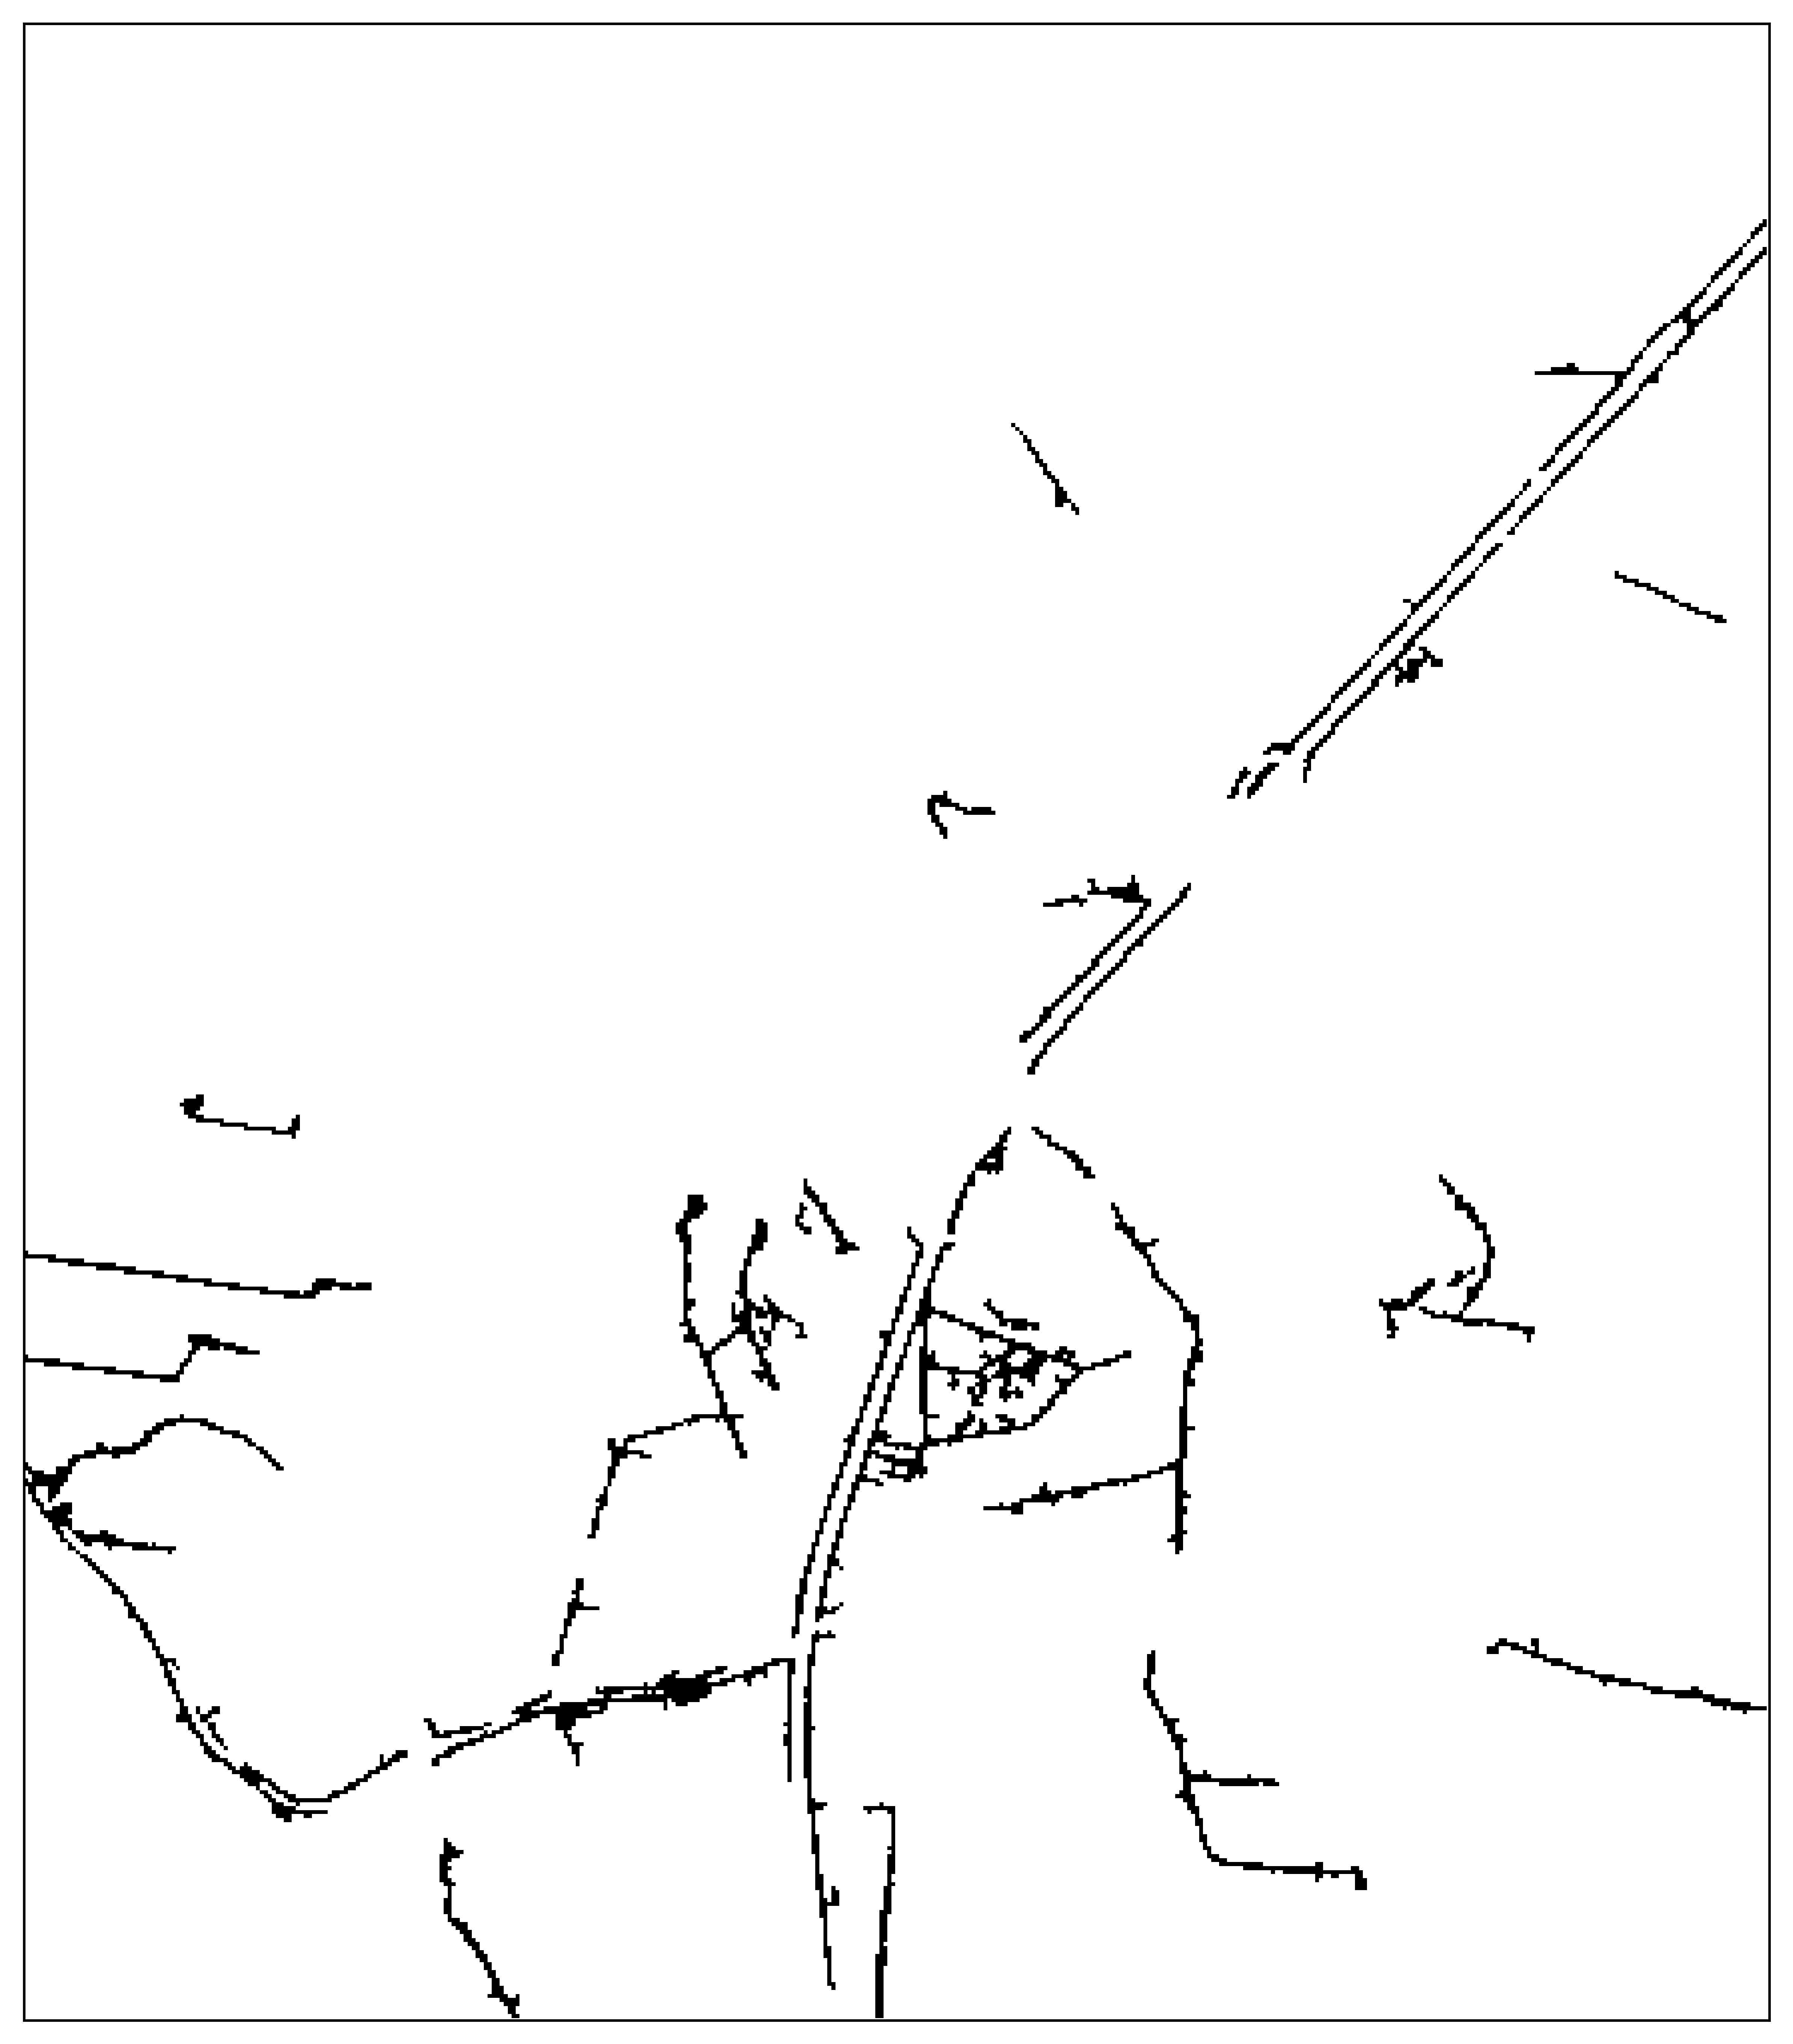
\includegraphics{./images/publ_post_process_step_6_lo.jpg}}}
    \caption{Step five and six of the post-process. Black pixels indicate a ditch prediction. \textbf{a: }Grid zone binarisation \textbf{b: }Cluster removal.}
    \label{fig:postprocessing3}
\end{figure}

\subsection{Evaluation} \label{evaluation}

Using only accuracy as an evaluation metric when dealing with an imbalanced dataset (roughly 98 \% of all pixels are non-ditch) would produce a poor performance assessment \citep{balanced}; by simply classifying all pixels as non-ditches, we would by default attain 98 \% accuracy. For this reason, the results were mainly evaluated using Cohen's Kappa (Cohen's $\kappa$) index, and the Area under Precision-Recall curve. Cohen's $\kappa$ index measures how much better a prediction is compared to a completely random prediction, where random would yield a value of zero \citep{kappa123}. With our data, a $\kappa$ value close to zero would be attained by predicting 2 \% of the occurrences as ditch pixels completely at random. Values above zero are better than random, and values below zero are worse than random.

The random rating $P_c$ of a prediction of $n$ occurrences is calculated with:\footnote{ P = Positive (ditch pixel), N = Negative (non-ditch pixel), T = true, F = false}

$$
P_c = \frac{\left(\frac{(TP + FN) \cdot (TP + FP)}{n}\right) + \left(\frac{(FN + TN) \cdot (FP + TN)}{n}\right)}{n}
$$

$$
\text{Cohen's } \kappa \text{ is then calculated as a value between -1 and 1 with:}
$$
$$\kappa = \frac{Accuracy - P_c}{1 - P_c}$$

The Precision-Recall curve and the Area under Precision-Recall curve (AUPRC) are additional metrics that can be used when evaluating datasets with a largely imbalanced class distribution \citep{precision_recall_curve}. The Precision-Recall curve has the recall value on the x-axis and the precision value on the y-axis, and the area under the curve that is defined by this point gives the AUPRC value. The area under this curve is given as a value between zero and one, where a value closer to one is better. The weighting causes the Precision-Recall curve to not place an equal value on true negatives and true positives \citep{precision_recall_curve}. For our ditch detection problem, this means that the AUPRC evaluation metric favours accurately classifying ditch pixels over accurately classifying non-ditch pixels.

To circumvent some of the performance evaluation issues arising from the use of pixel classification for ditch objects as well as not having completely accurate labels on a pixel basis (due to uncertainties in the width of the ditches), we modified the evaluation labels to allow for some error in close proximity to ditches in the prediction. False negatives and false positive grid zones that lay adjacent to the ditch label grid zones were evaluated as true negatives and true positives, as they can be considered a part of correctly located ditch objects (\hyperref[fig:newlabels]{Figure} \ref{fig:newlabels}).

\begin{figure} [!htb]
    \centering
    \subfigure[]{
        \resizebox*{6.5cm}{!}{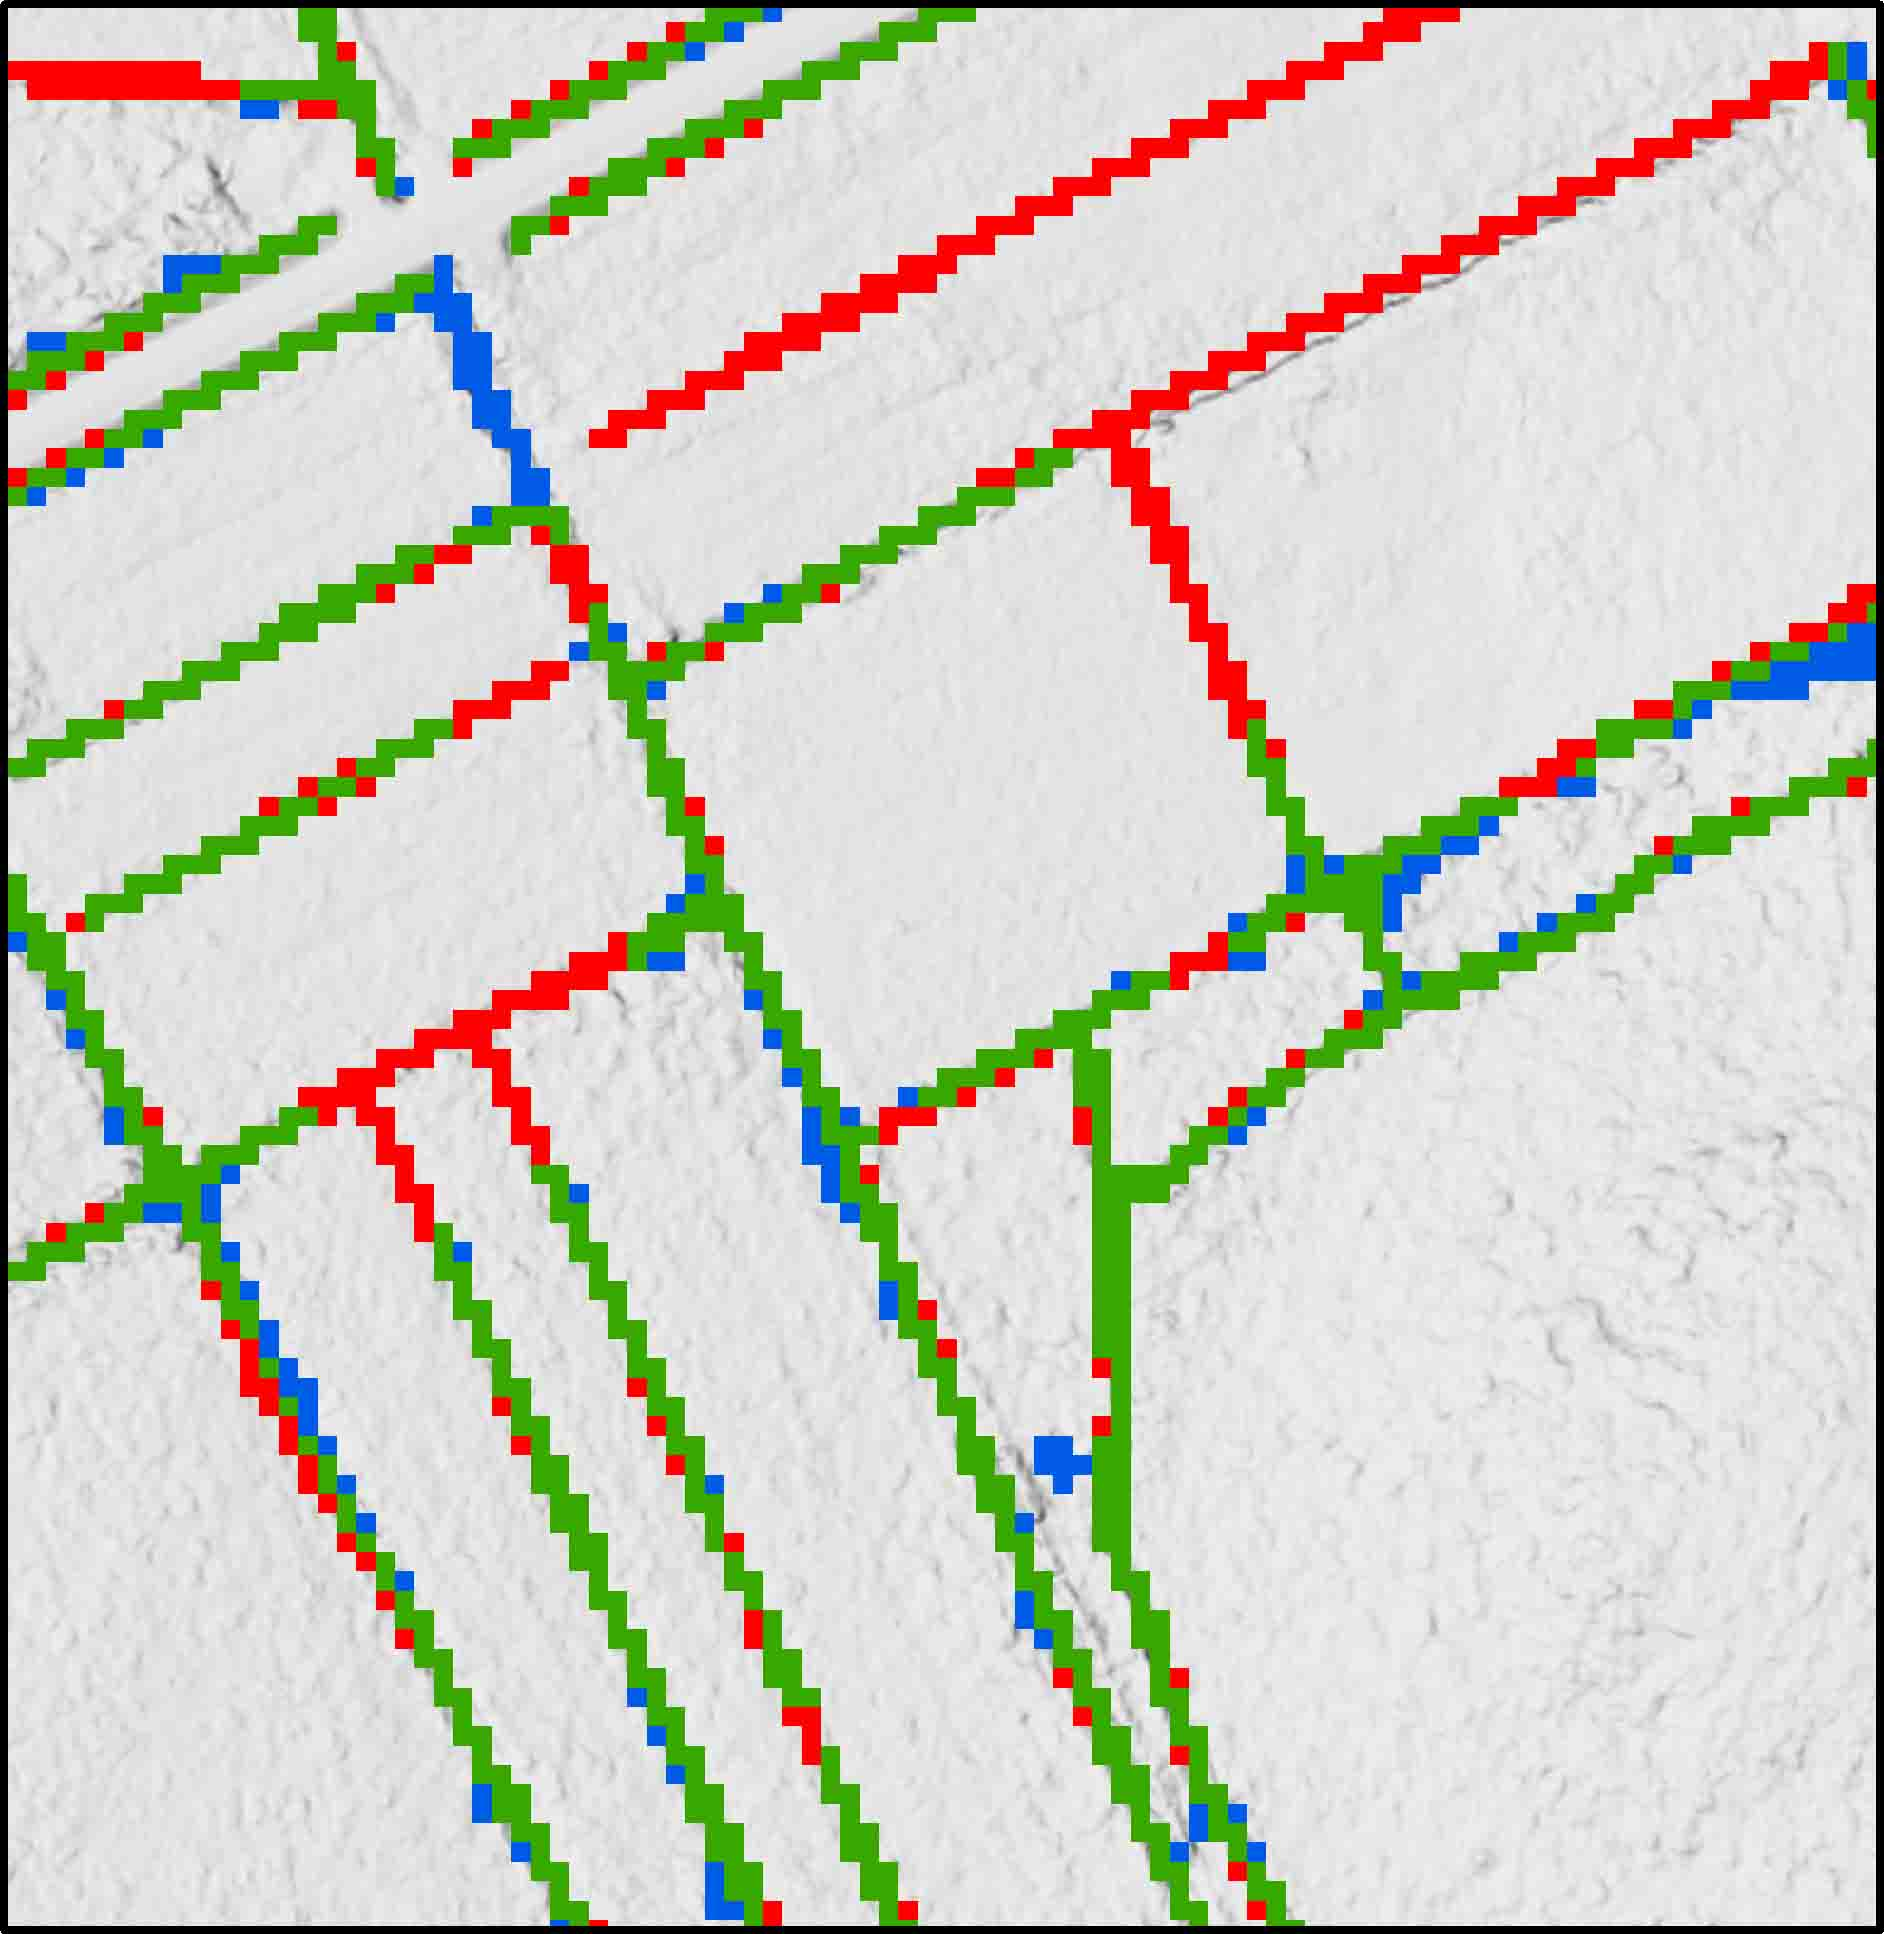
\includegraphics{./images/re_evaluation_1_lo.jpg}}}\hspace{5pt}
    \subfigure[]{
        \resizebox*{6.5cm}{!}{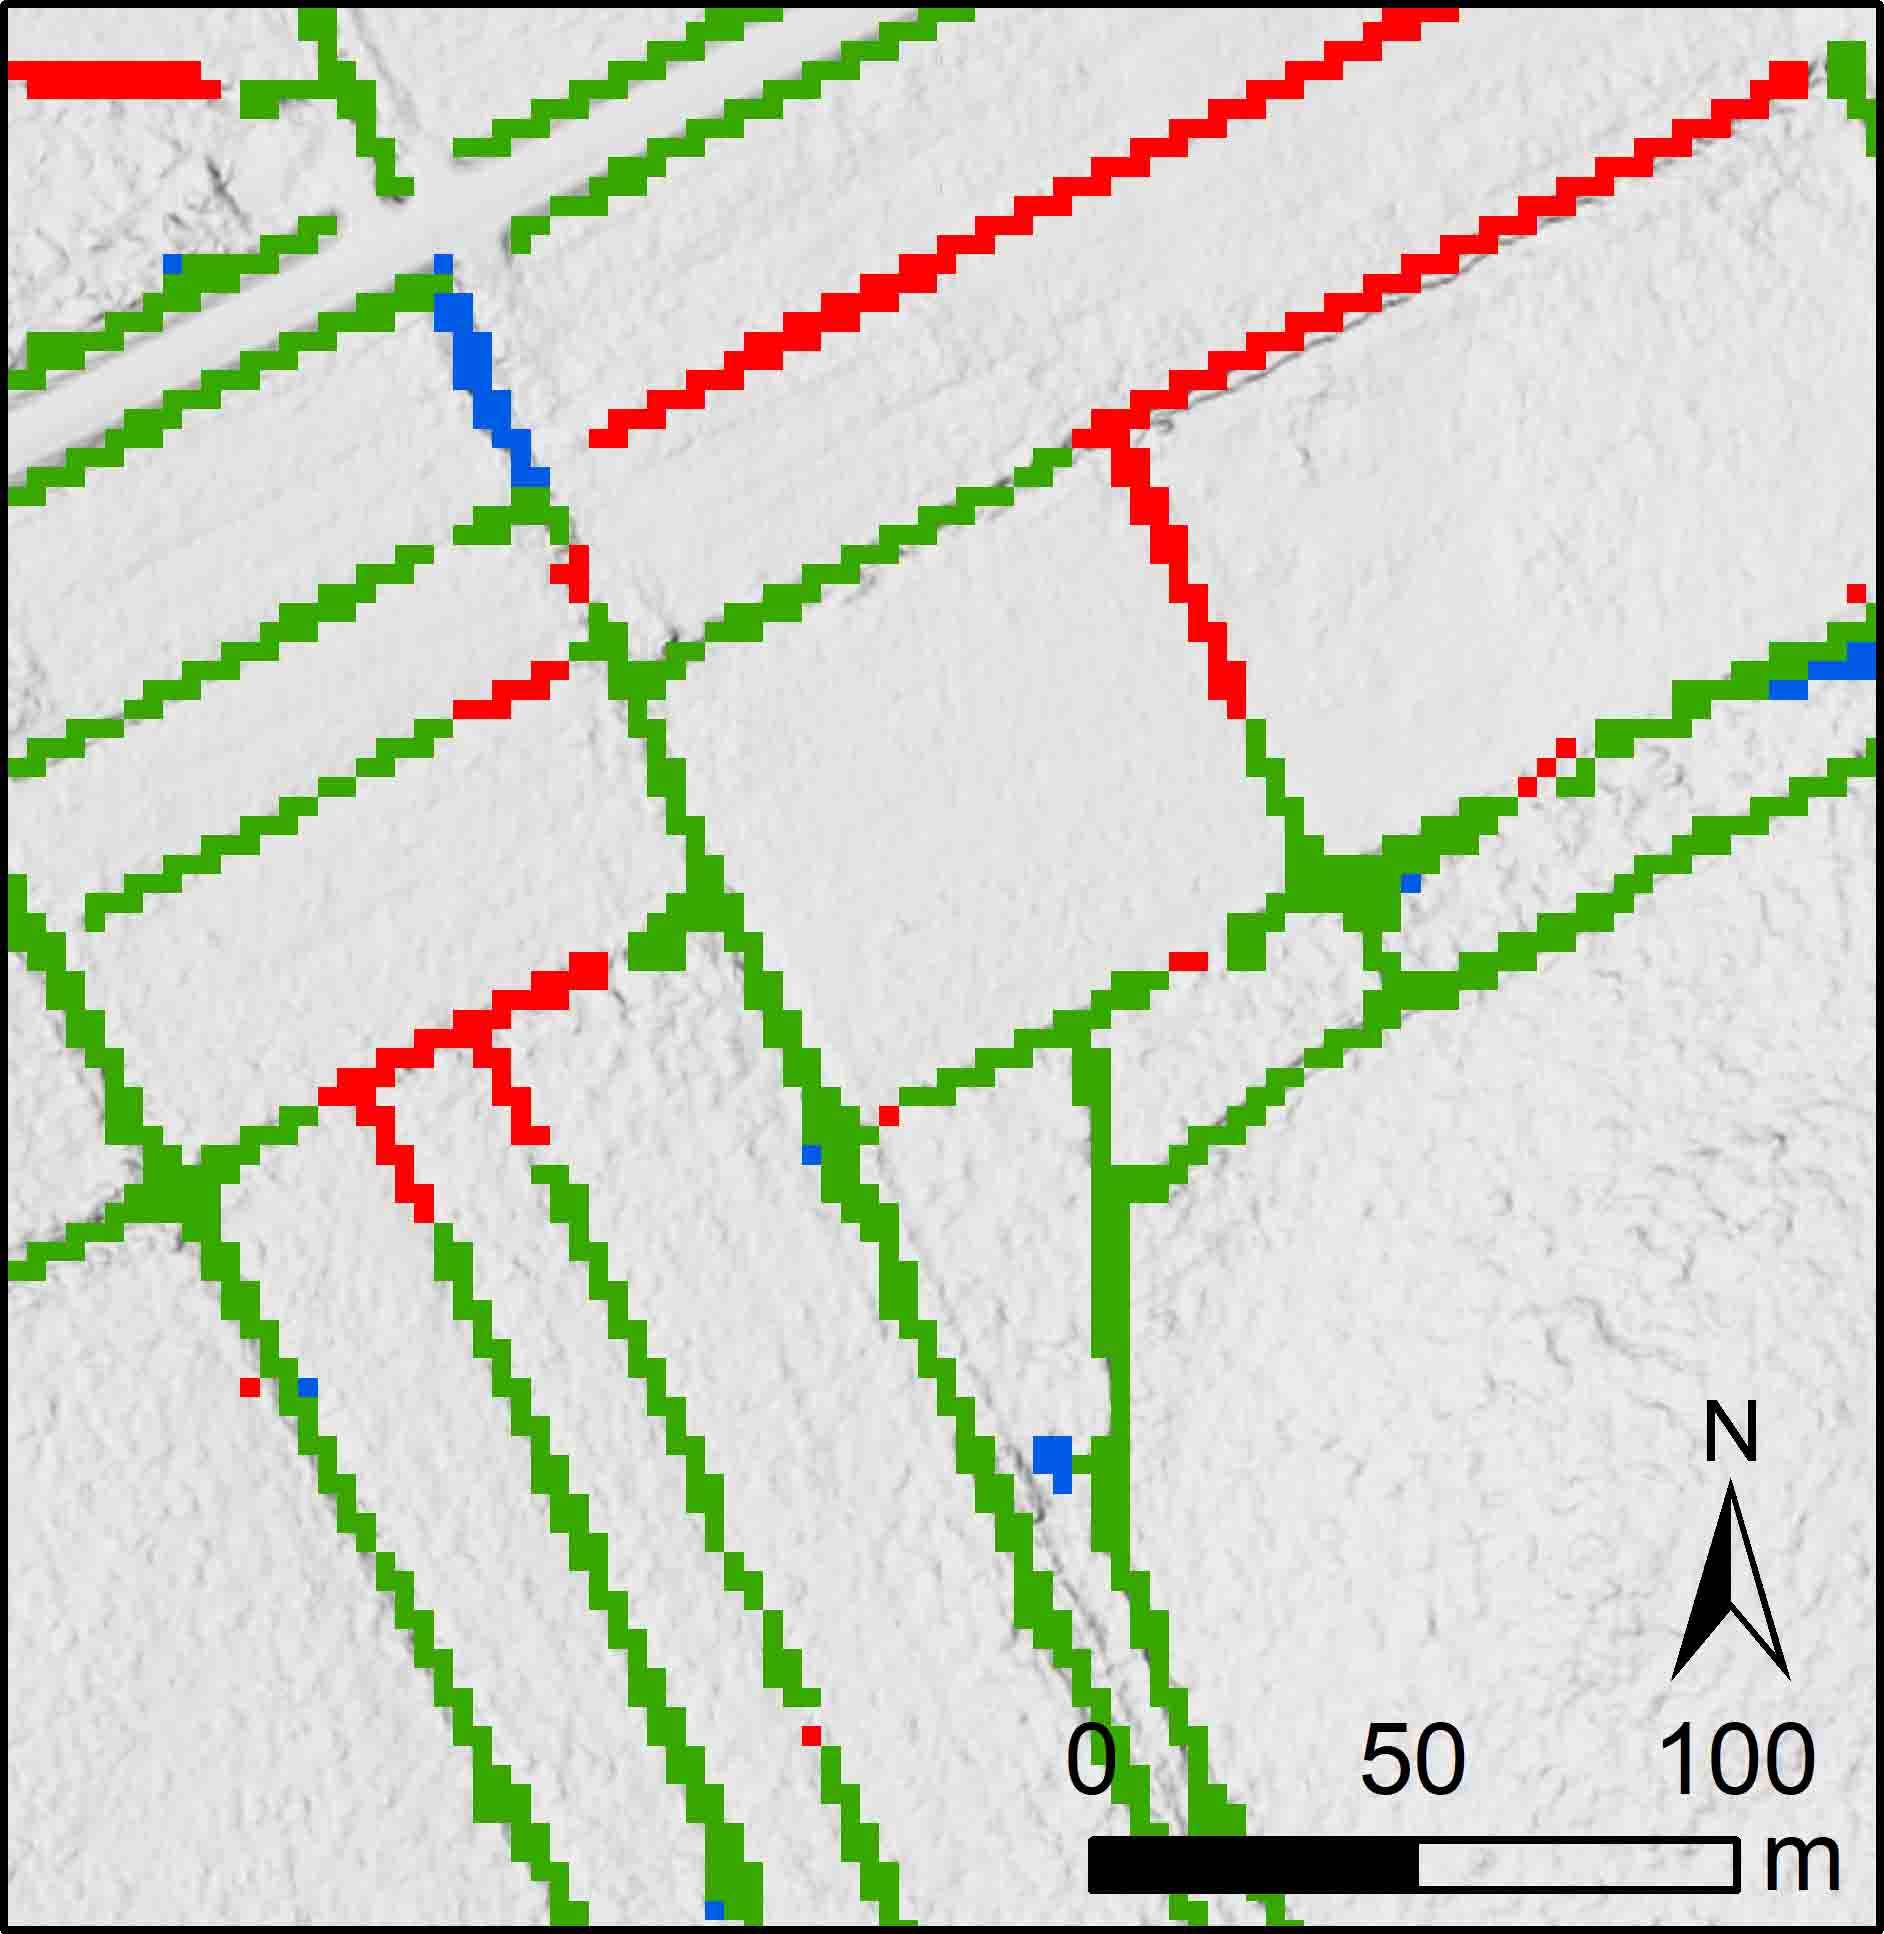
\includegraphics{./images/re_evaluation_2_lo.jpg}}}
    \caption{Illustration of the modified evaluation labels. Green marks true positives, red marks false negatives, and blue marks false positives. False positives and false negatives that lay within one grid zone (9 $m^2$) of a ditch label were evaluated as true positives and true negatives. \textbf{a:} Original results, \textbf{b:} Modified results. }
    \label{fig:newlabels}
\end{figure}

\section{Results and analysis}
In the national survey (NILS), a total of 1103 natural watercourses, 131 straightened watercourses/channels, and 2089 ditches were found in the field. This simple investigation highlights two things: Firstly, the ditches make up the majority of the small scale water channels in the Swedish landscape; almost twice as many as the natural streams. Secondly, most of the small scale channels are missing on the current maps; only 45 \% of the natural watercourses, 25 \% of the straightened watercourses/channels, and 9 \% of the ditches were mapped (\hyperref[fig:watercoursebarplot]{Figure} \ref{fig:watercoursebarplot}).

\begin{figure}[htb]
    \centering
    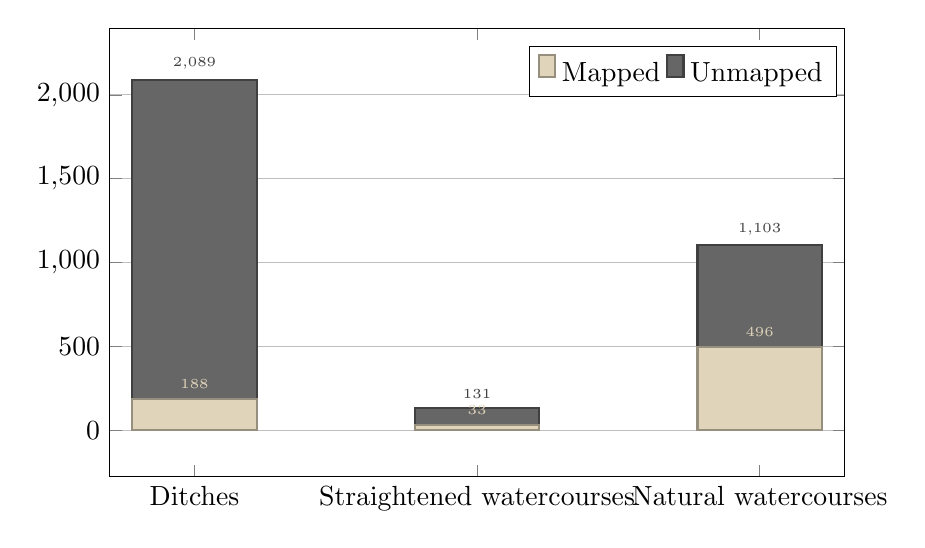
\begin{tikzpicture}
    \begin{axis}[
        width={0.9\textwidth},
        height={0.6\textwidth},
        ylabel={fluorescence},
        ybar stacked,
        ymajorgrids=true,
    	bar width=45pt,
    	nodes near coords,
    	every node near coord/.append style={font=\tiny},
        enlarge y limits={0.15},
        enlarge x limits=0.15,
        legend style={at={(0.78,0.96)},
          anchor=north,legend columns=-1},
        ylabel={{}},
        symbolic x coords={Ditches, Straightened  watercourses, Natural  watercourses},
        xtick=data,
        ytick={0,500,1000,1500,2000},
        x tick label style={rotate=0,anchor=north},
        ]
    \addplot+[ybar,color=custombeige,fill=custombeige,draw=custombeigeouter,thick] plot coordinates {(Ditches,188) (Straightened  watercourses,33) 
      (Natural  watercourses,496)};
    \addplot+[ybar,color=customgrayouter,fill=customgray,draw=customgrayouter,thick] plot coordinates {(Ditches,1901) (Straightened  watercourses,98) 
      (Natural  watercourses,607)};
    \legend{\strut Mapped, \strut Unmapped}
    \end{axis}
    \end{tikzpicture}
    \caption{The bars indicate the number of observed channels in the National Inventory of Landscapes in Sweden's (NILS) line inventory of small watercourses (width $<$ 6 m). The colours of the bars indicate if they are mapped or not on the Swedish Property map.}
    \label{fig:watercoursebarplot}
\end{figure}



\hyperref[recreatedpredictionperformance]{Table} \ref{recreatedpredictionperformance} shows the evaluation metrics from the experiments with the digital terrain indices separately. Of the four, the Impoundment Index and the HPMF index performed relatively close to each other and outperformed the other indices for most of the metrics.

\begin{table}[!htb]
    \tbl{Metrics from the total results of the four digital terrain indices experiments.}
    {\begin{tabular}{lcccc} \toprule
        Metric & Sky View Factor & Impoundment & HPMF & Slope\\ \midrule
        Accuracy \%     & 83.67 & 97.07 & 97.45 & 82.66 \\
        Recall \%       & 44.54 & 29.98 & 25.31 & 34.83 \\
        Precision \%    &{ 4.00}  & 18.51 & 20.10 & { 2.99} \\
        $\kappa$ rating & 0.048 & 0.215 & 0.211 & 0.029 \\
        AUPRC & 0.247 & 0.248 & 0.232 & 0.194 \\ \bottomrule
    \end{tabular}}
    \label{recreatedpredictionperformance}
\end{table}

\hyperref[predictionperformance]{Table} \ref{predictionperformance} displays all the evaluation metrics for the prediction of our method. The confidence intervals were calculated from the 11 different subsections that the experiment was performed on. Because the subsections have varying amounts of ditches in them, the confidence intervals will not be completely accurate, but will produce a close estimation.

From \hyperref[predictionperformance]{Table} \ref{predictionperformance}, it is observed that averaging the results from the 11 subsections would yield a very similar value to the total results, indicating that the ditch detector generally performs equally well on subsections with a small amount of ditches as on subsections with a large amount of ditches.

\begin{table}[!htb]
    \tbl{Metrics for the prediction performance of our ditch detector.}{\begin{tabular}{lccc} 
        \toprule
        Metric & Total\textsuperscript{a} & Subsection\textsuperscript{b}& CI 95\%\textsuperscript{c} \\ 
        &&Average&\\ \midrule
        Accuracy     \% & 99.00 & 99.00 & [98.69 , 99.32] \\
        Recall       \% & 70.28 & 70.19 & [61.28 , 79.09] \\
        Precision    \% & 77.38 & 75.79 & [71.94 , 79.64] \\
        $\kappa$ rating & 0.732 & 0.718 & [0.655 , 0.781] \\
        AUPRC           & 0.741 & 0.733 & [0.674 , 0.791] \\ 
        \bottomrule
    \end{tabular}}
    \tabnote{
        \textsuperscript{a} The result of all 11 subsection experiments when combined. \newline
        \textsuperscript{b} An average score from the 11 different subsections that the experiment was performed on. \newline
        \textsuperscript{c} Confidence intervals at 95 \% confidence level.}
    \label{predictionperformance}
\end{table}

The $\kappa$ rating for our method can be seen in the \textit{Total} column in \hyperref[predictionperformance]{Table} \ref{predictionperformance} ($\kappa$ = 0.732). The $\kappa$ ratings from the four digital terrain indices experiments can be seen in  \hyperref[recreatedpredictionperformance]{Table} \ref{recreatedpredictionperformance} ($\kappa$ = 0.048, $\kappa$ = 0.215, $\kappa$ = 0.211, $\kappa$ = 0.029). Because the $\kappa$ rating from our method outperforms all digital terrain indices, our hypothesis has been confirmed by the experiments. Most false positives lie in stream channels (\hyperref[fig:resultsillustrations]{Figure} \ref{fig:resultsillustrations} \hyperref[fig:resultsillustrations]{a, b}) and most false negatives occurred either due to ditches being too shallow (\hyperref[fig:resultsillustrations]{Figure} \ref{fig:resultsillustrations} \hyperref[fig:resultsillustrations]{c, d}), or due to the attempt at removing streams using the input variables as explained in \ref{impoundmentstreamremoval} removing the deepest ditches  (\hyperref[fig:resultsillustrations]{Figure} \ref{fig:resultsillustrations} \hyperref[fig:resultsillustrations]{e, f}).

\begin{figure} [!htb]
    \centering
    \subfigure[]{
        \resizebox*{5.5cm}{!}{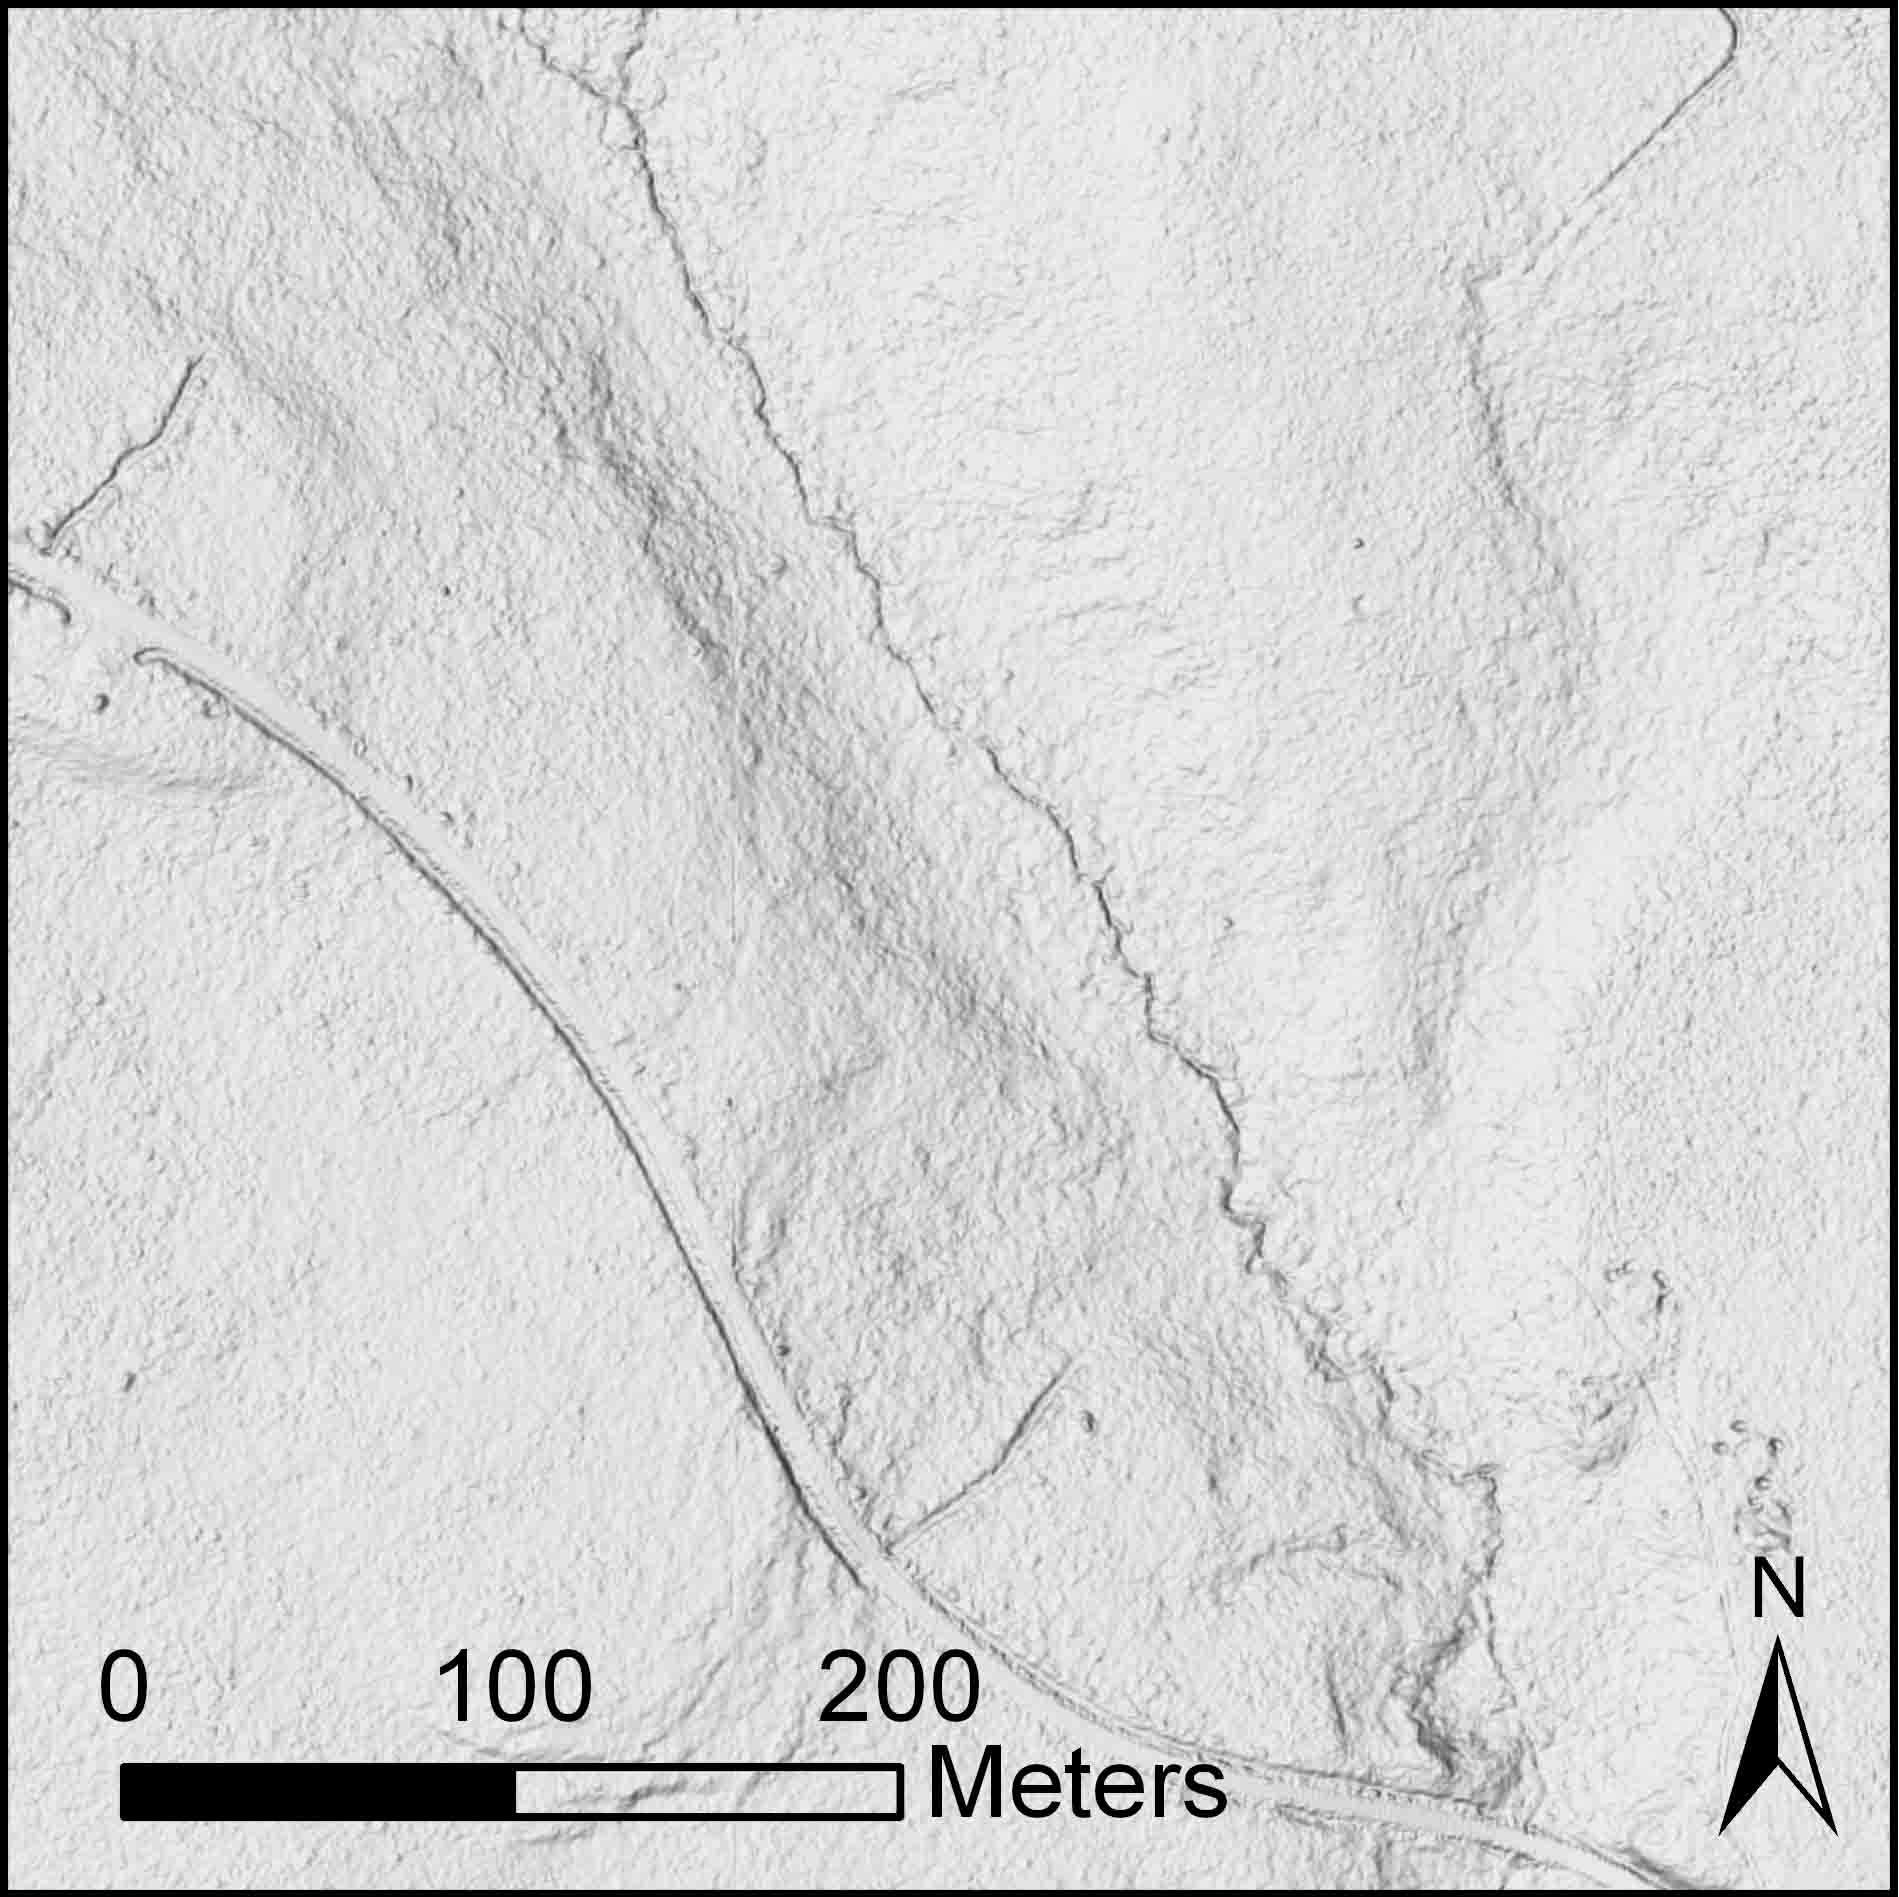
\includegraphics{./images/results_illustration_1_lo.jpg}}}\hspace{5pt}
    \subfigure[]{
        \resizebox*{5.5cm}{!}{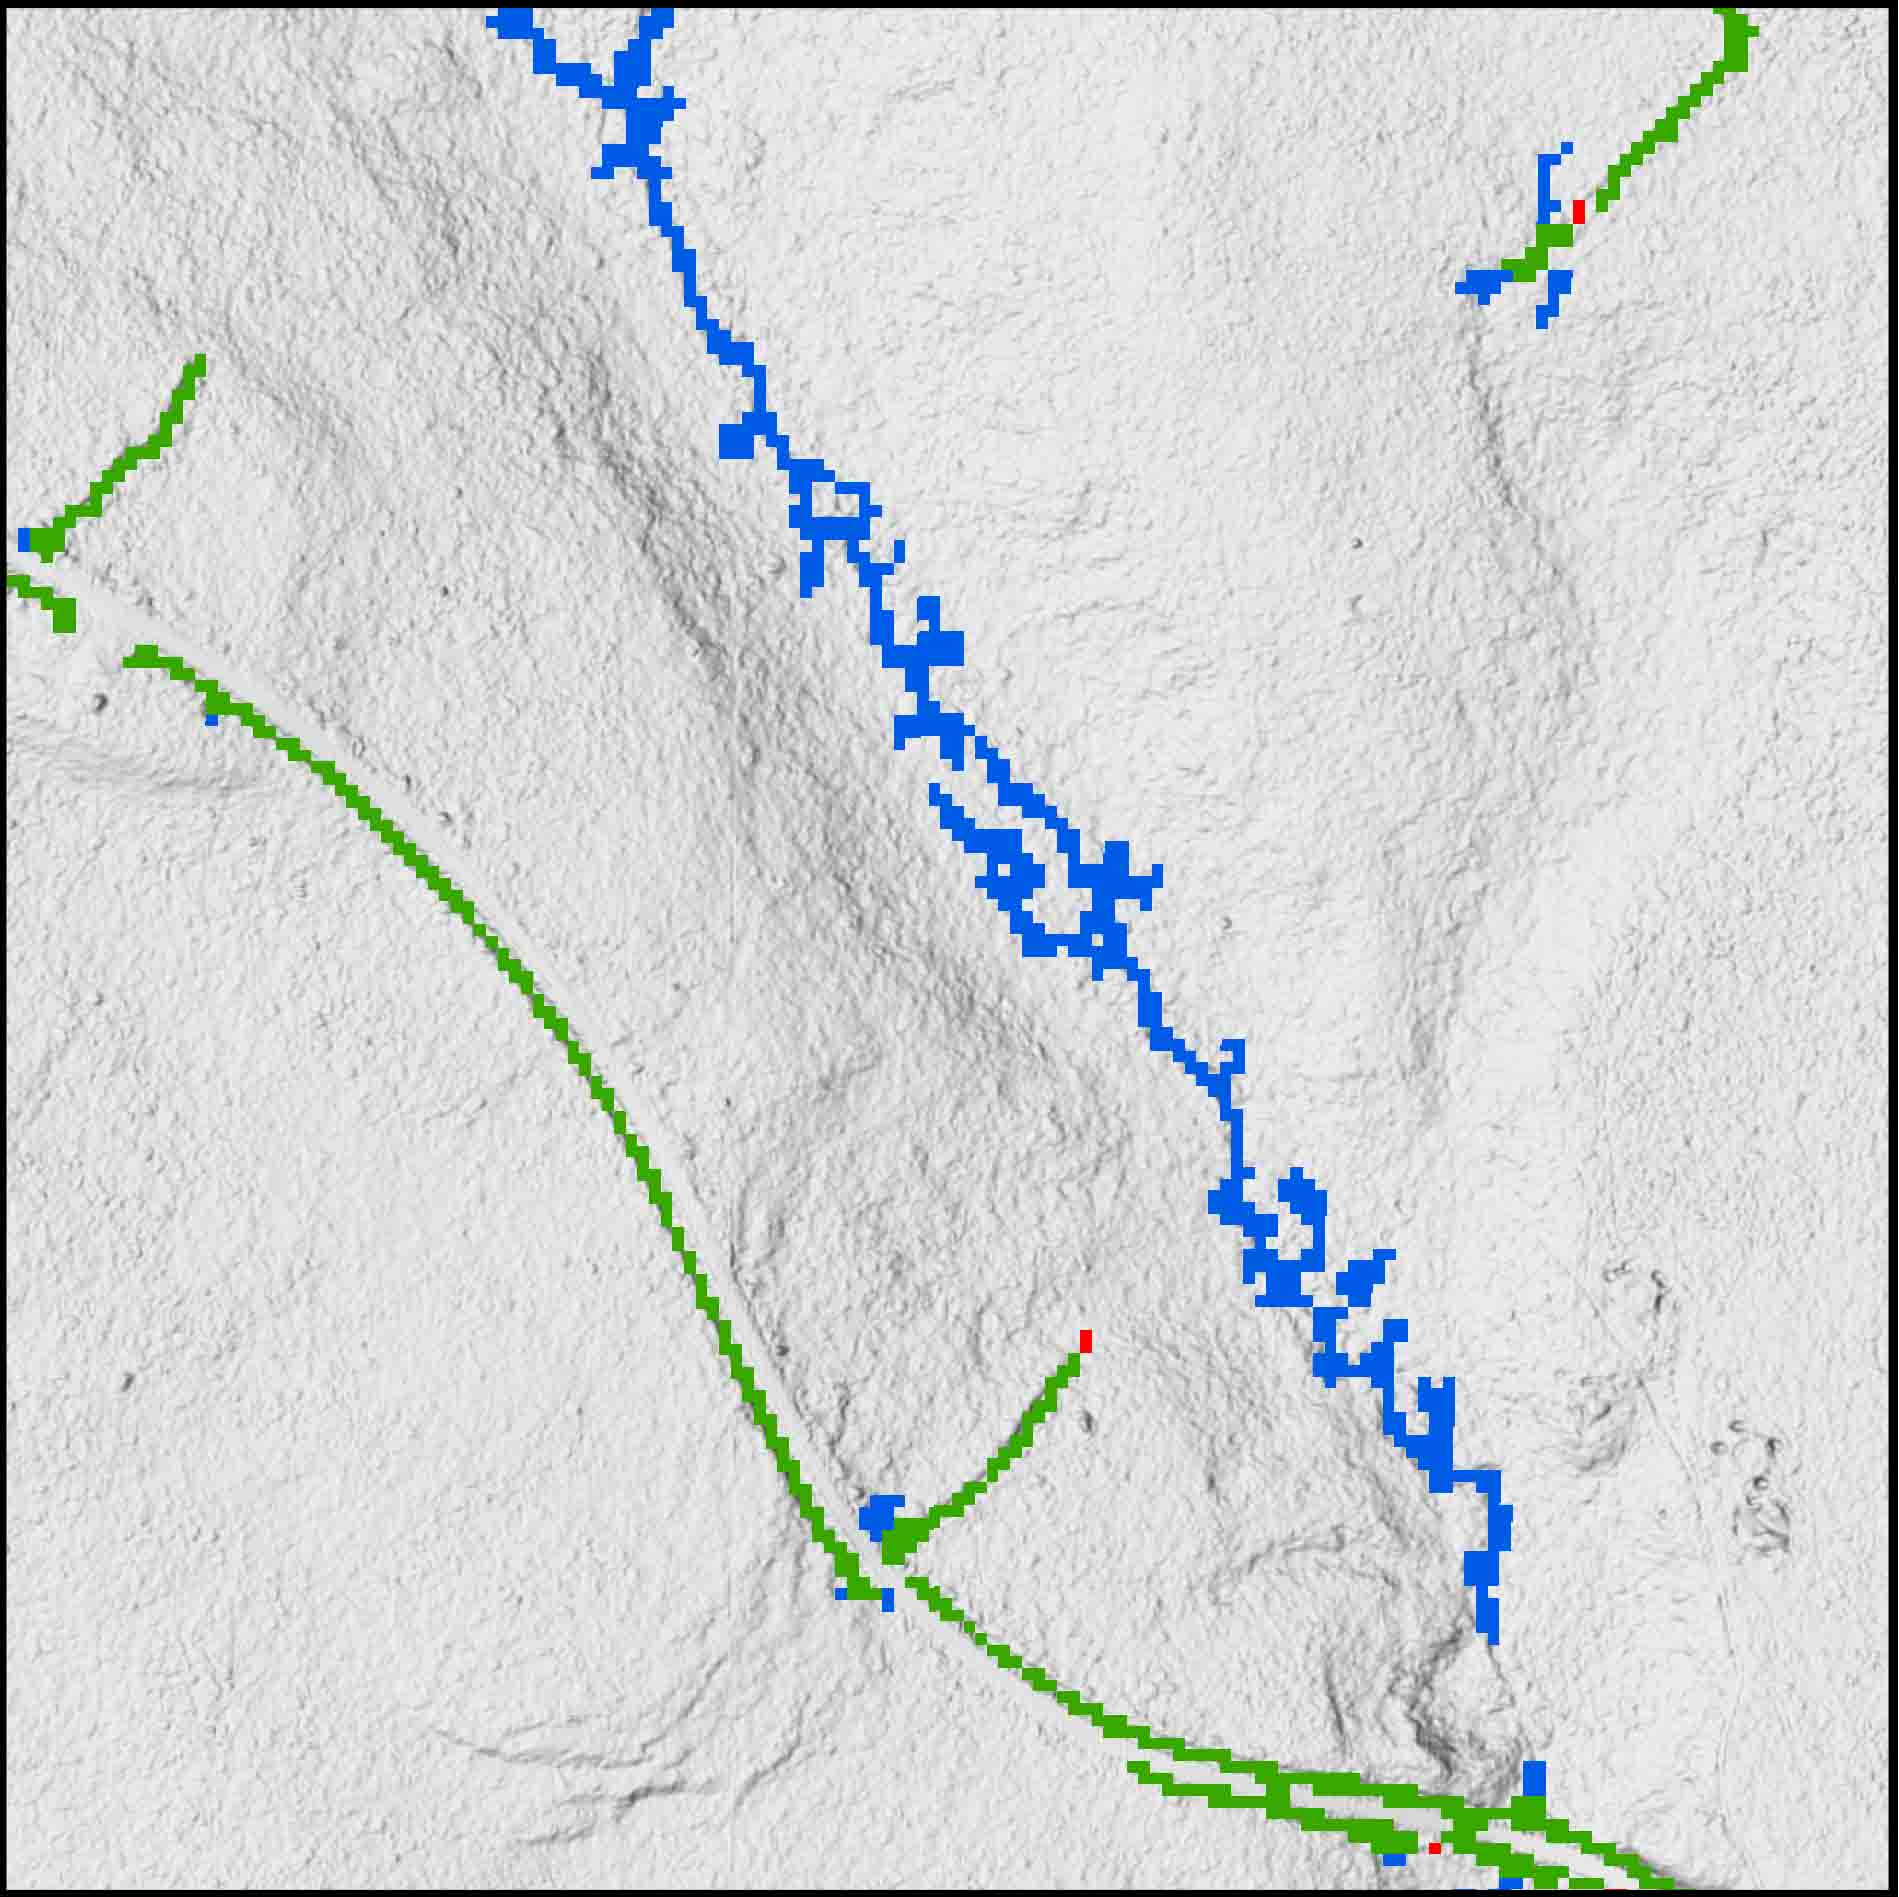
\includegraphics{./images/results_illustration_2_lo.jpg}}}
    \subfigure[]{
        \resizebox*{5.5cm}{!}{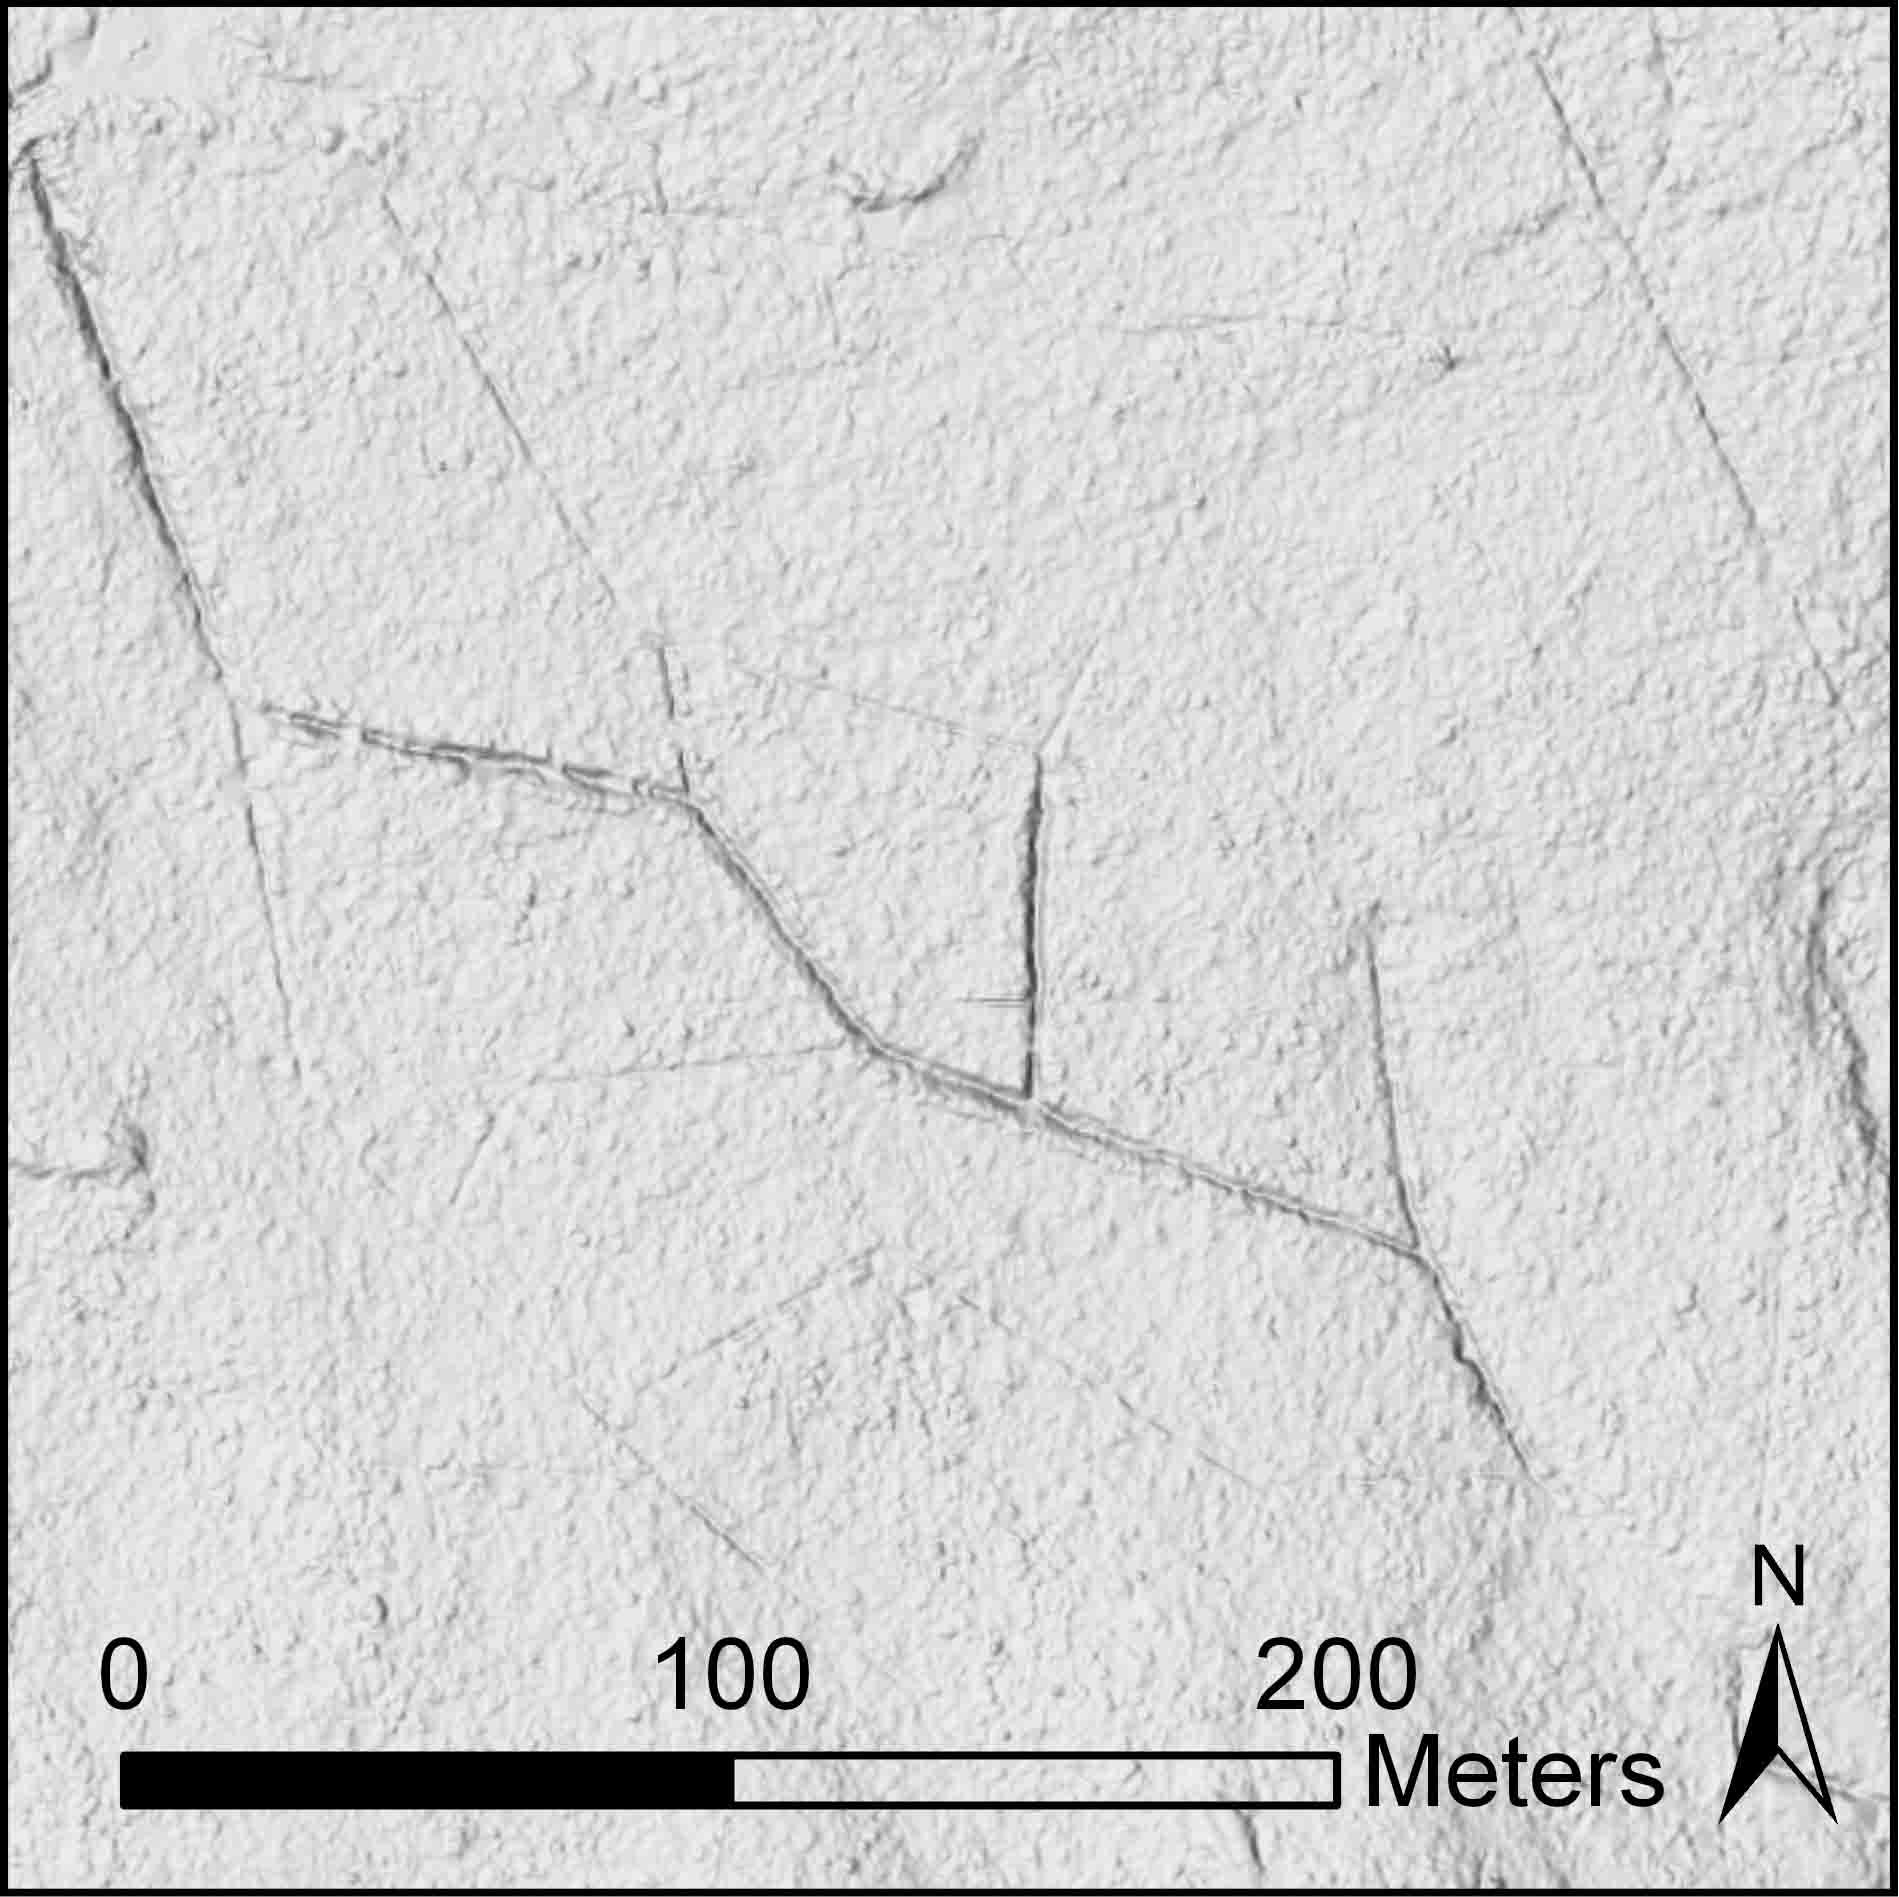
\includegraphics{./images/results_illustration_3_lo.jpg}}}\hspace{5pt}
    \subfigure[]{
        \resizebox*{5.5cm}{!}{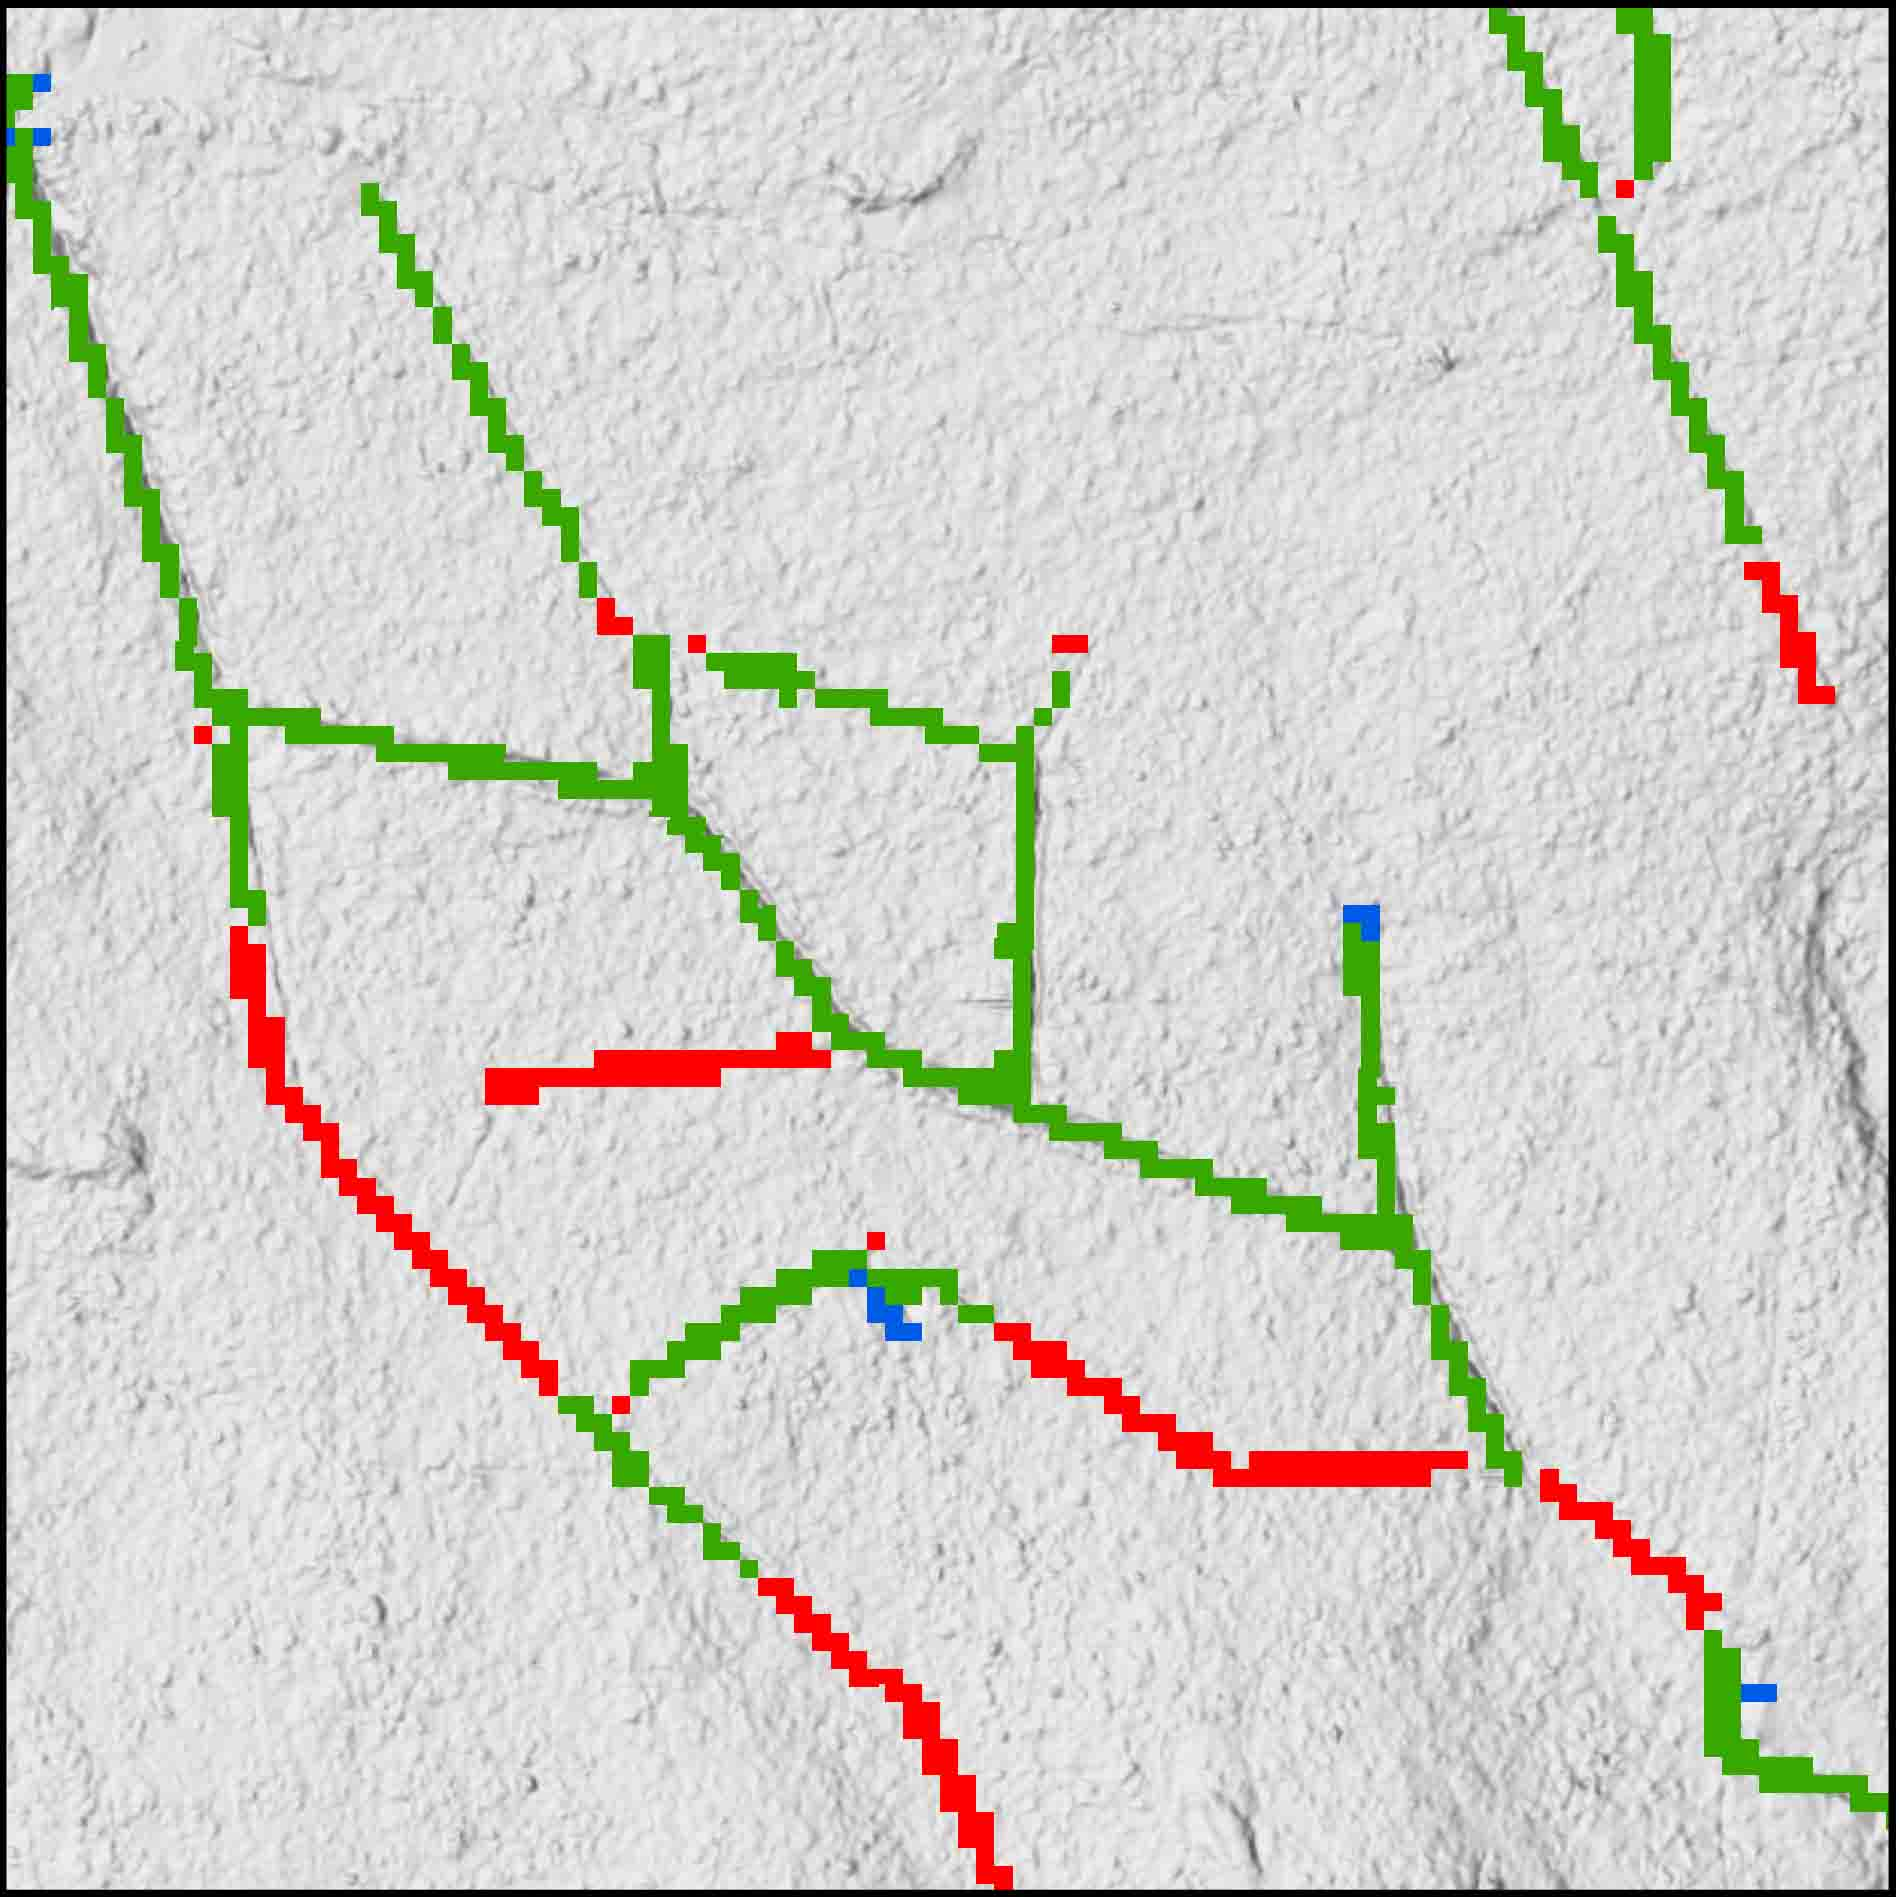
\includegraphics{./images/results_illustration_4_lo.jpg}}}
    \subfigure[]{
        \resizebox*{5.5cm}{!}{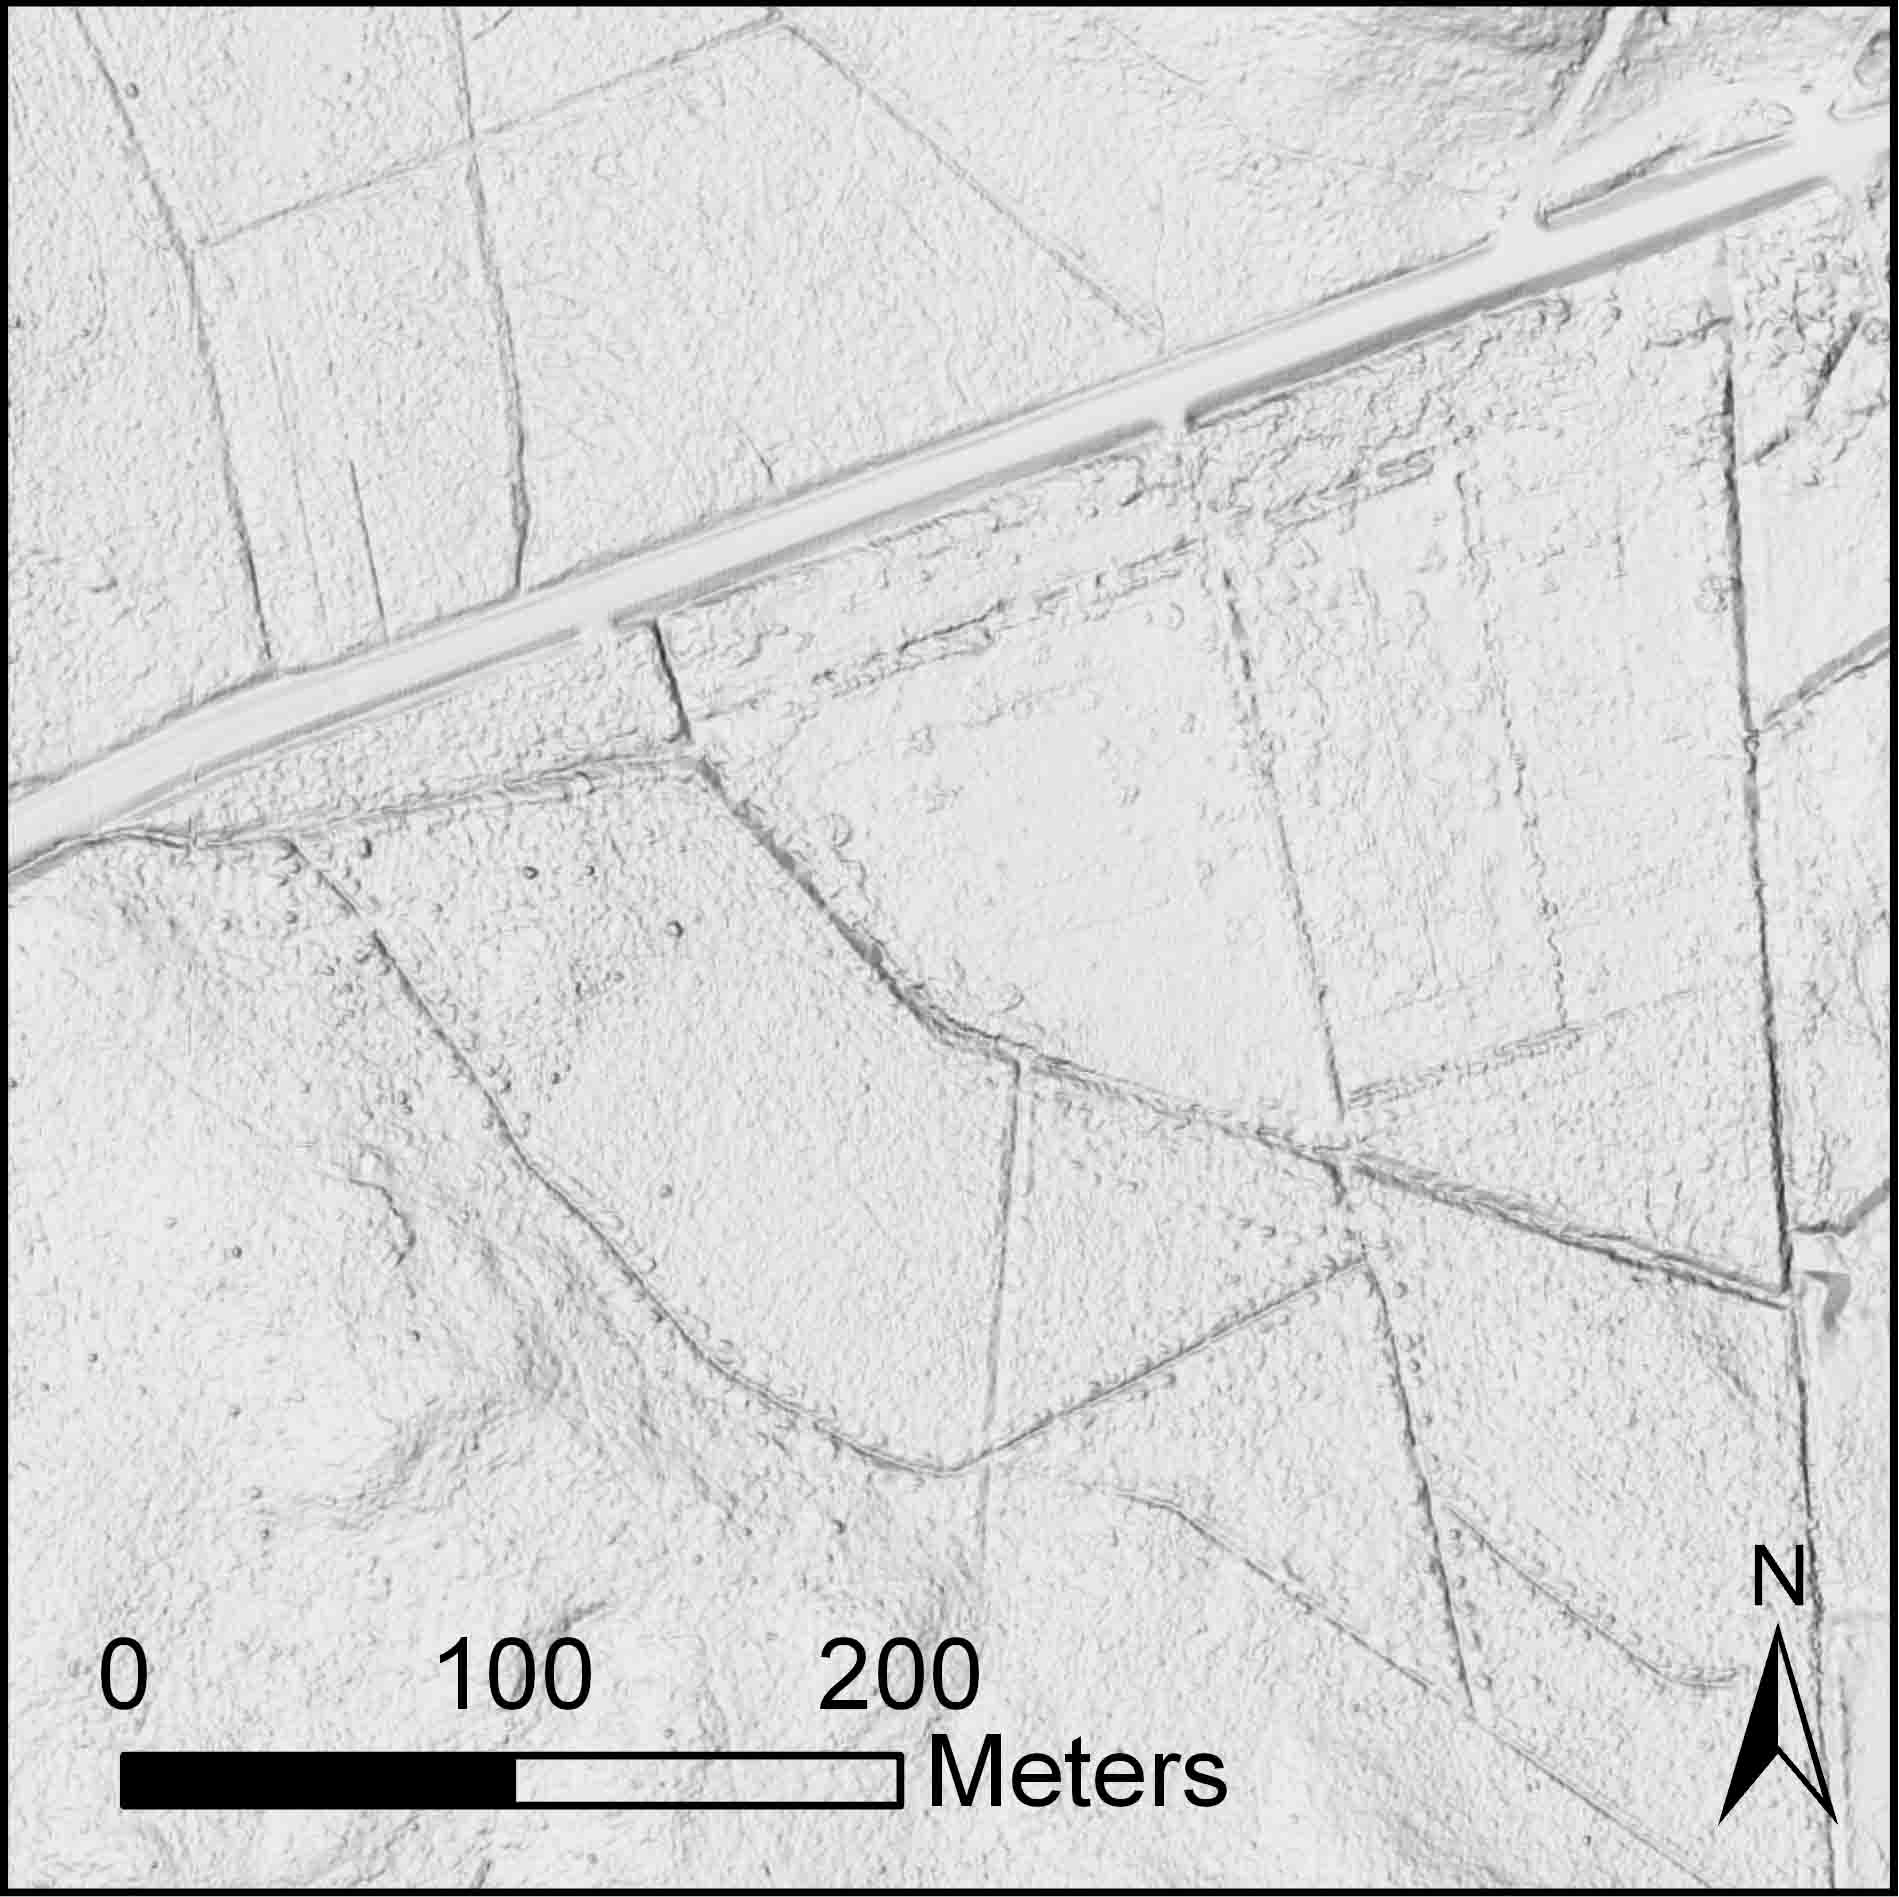
\includegraphics{./images/results_illustration_5_lo.jpg}}}\hspace{5pt}
    \subfigure[]{
        \resizebox*{5.5cm}{!}{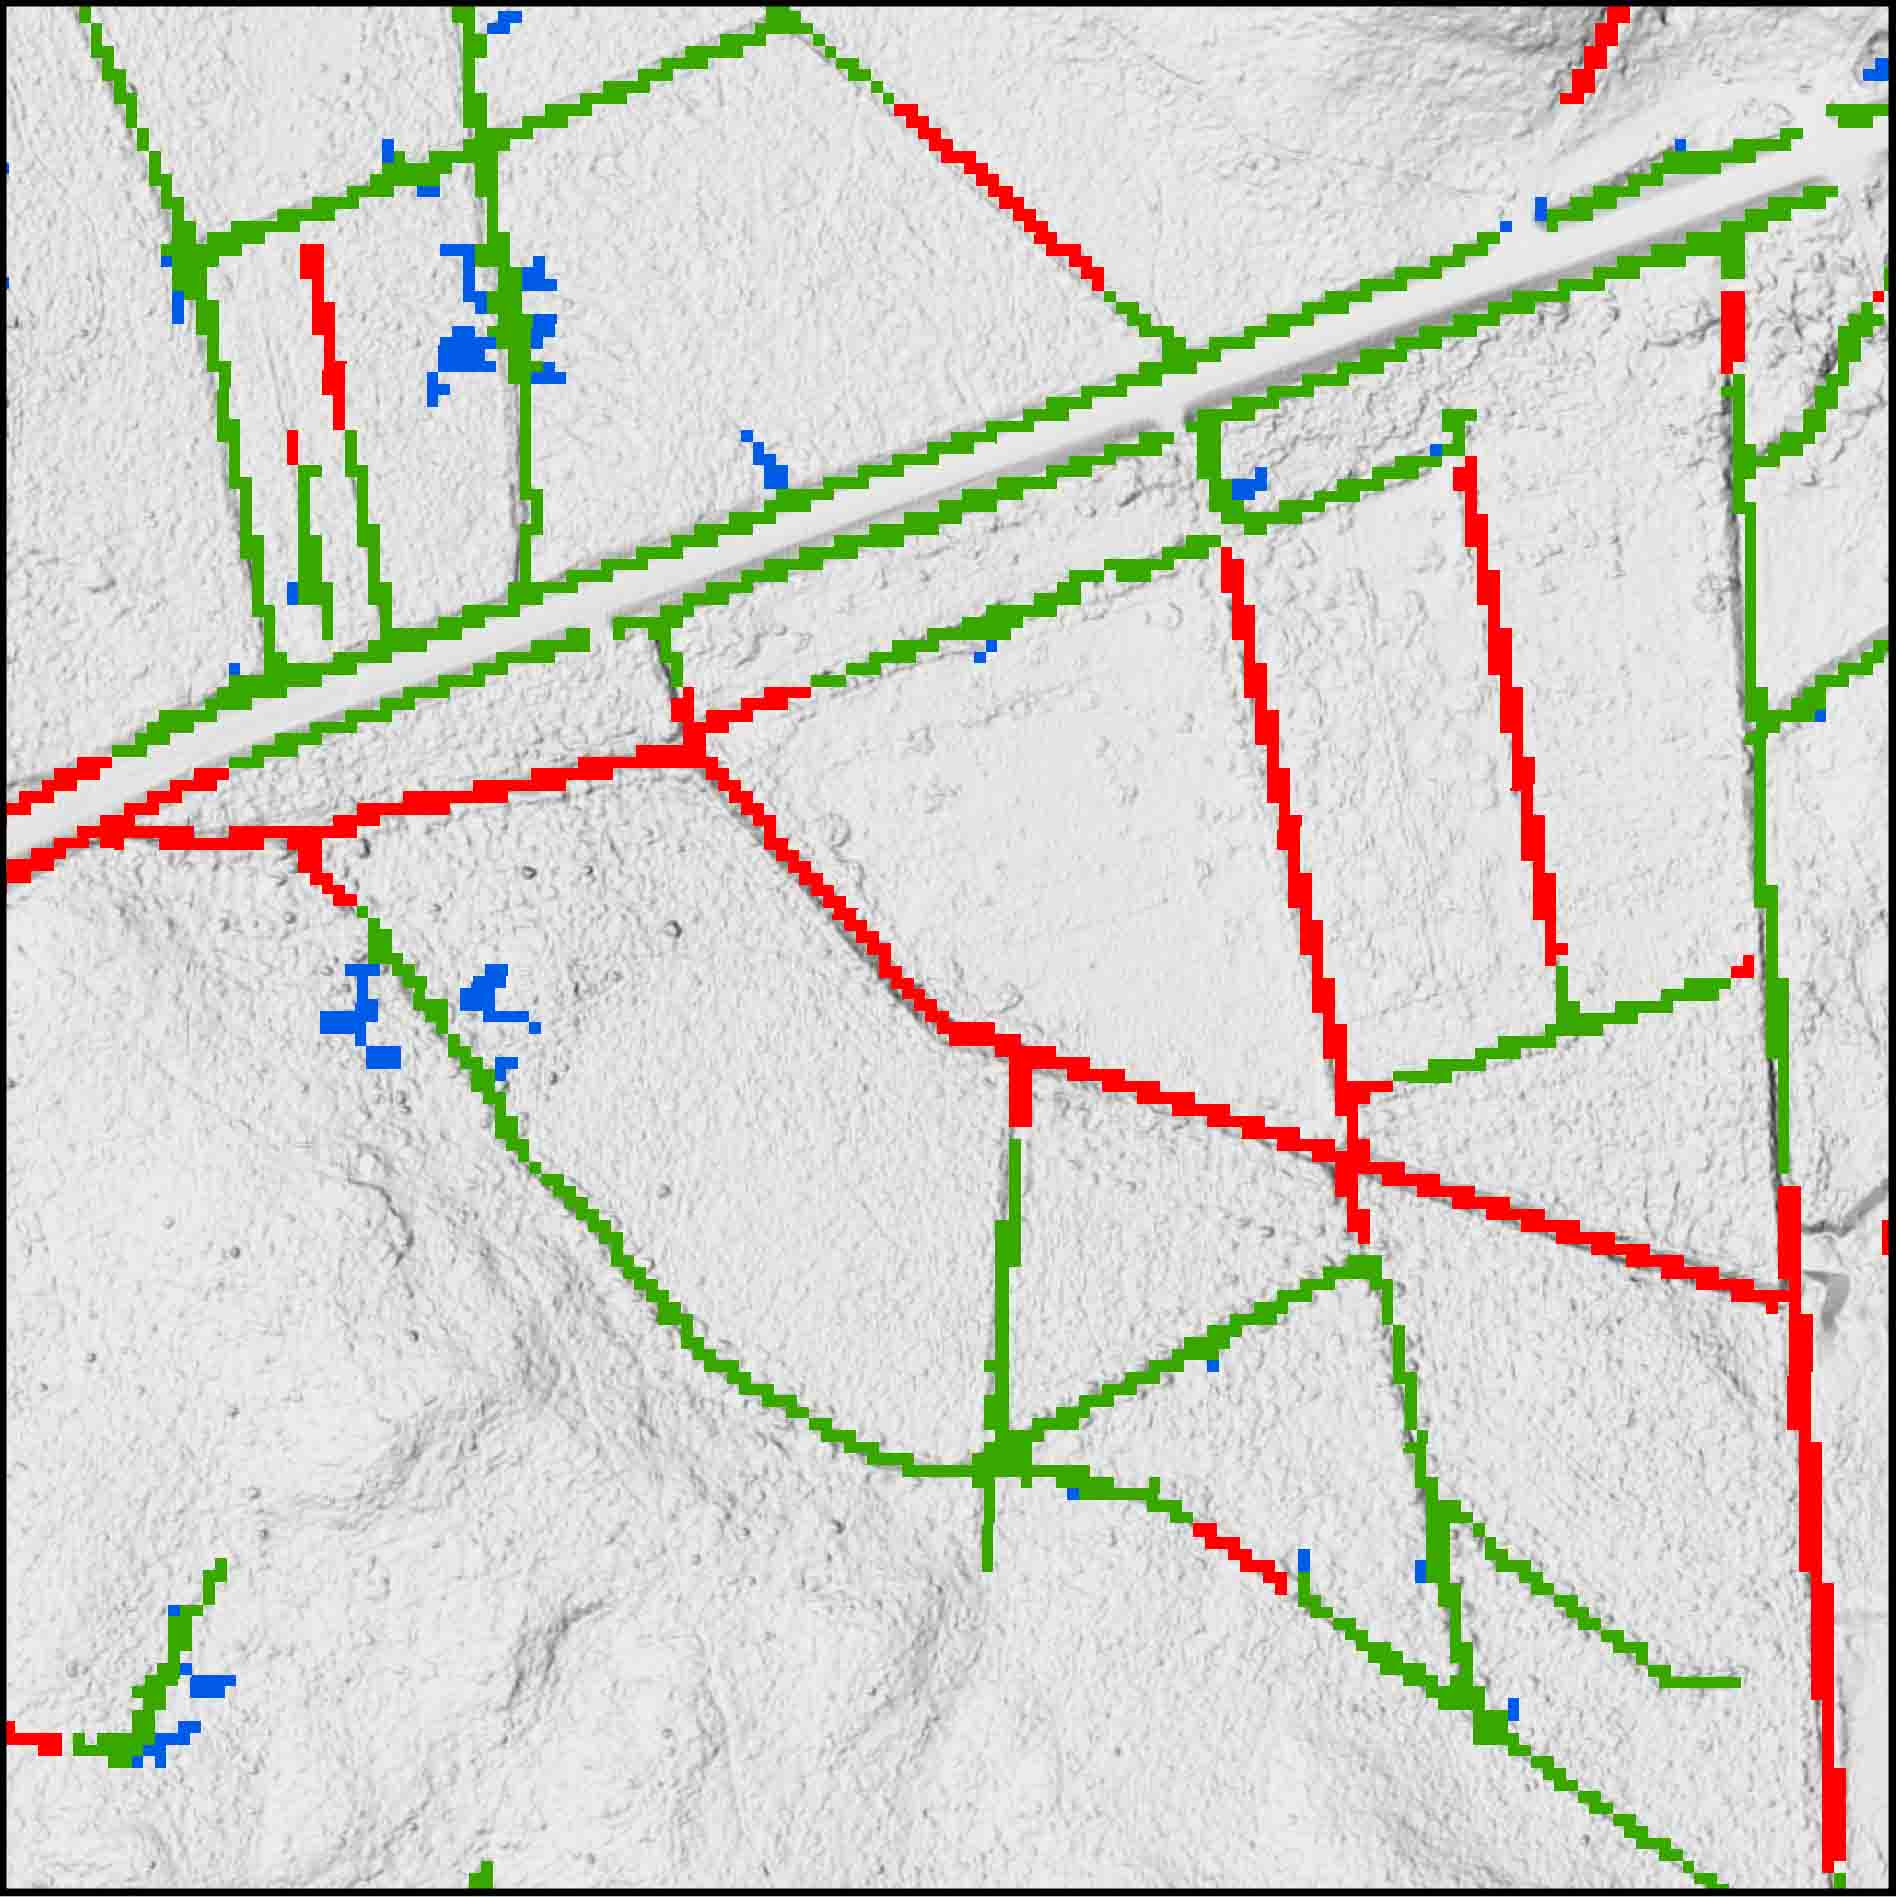
\includegraphics{./images/results_illustration_6_lo.jpg}}}
    \caption{The left panel shows the hillshade for a number of subsections, and the right panel shows the hillshade with the extracted ditches superimposed on top. Green marks correctly classified ditches (true positives), red marks missed ditches (false negatives), blue marks incorrectly classified ditches (false positives), and transparent areas mark correctly classified non-ditches (true negatives). \textbf{a} and \textbf{b} illustrate that the most common false positives were natural stream channels being classified as ditches. \textbf{c} and \textbf{d} illustrate that very shallow ditches that were barely visible in the DEM were not captured with our ditch detector. \textbf{e} and \textbf{f} illustrate that some of the deepest and more prominent ditches were also missed. This occurred as a result of attempting to get rid of more false positives in the form of streams by using the input variables, as explained in \ref{impoundmentstreamremoval}.}
    \label{fig:resultsillustrations}
\end{figure}
\clearpage


In \hyperref[featureimportancetable]{Table} \ref{featureimportancetable}, the top 20 (out of 40) input variables from the Random Forests models are presented with their importance percentages for the models making a successful prediction. Input variables based on HPMF and Impoundment Index contributed the most to a successful prediction. The Gini importance was obtained using the Gini impurity for each variable \citep{gini}.

\begin{table} [!htb]
    \tbl{The top 20 input variables (out of 40) by importance when the models make a prediction.}
        {\begin{tabular}{llr}
          \toprule
          Position & Variable\textsuperscript{a} & Importance (\%) \\ \midrule
          1.  & Impoundment mean 3                                  & 7.33\\
          2.  & HPMF mean 4                                         & 6.23\\
          3.  & Impoundment mean 4                                  & 5.57\\
          4.  & Impoundment mean 2                                  & 5.41\\
          5.  & HPMF mean 3                                         & 4.33\\
          6.  & Impoundment median 4                                & 3.84\\
          7.  & HPMF Gabor - streams removed                        & 3.54\\
          8.  & HPMF median 4                                       & 3.40\\
          9.  & Impoundment median 2                                & 3.01\\
          10. & Sky View Factor Gabor - streams removed             & 2.84\\
          11. & HPMF mean 6                                         & 2.73\\
          12. & Impoundment median 6                                & 2.69\\
          13. & Impoundment standard deviation 4                    & 2.52\\
          14. & Sky View Factor Gabor                               & 2.44\\
          15. & Impoundment ditch amplification                     & 2.43\\
          16. & Impoundment mean 6                                  & 2.27\\
          17. & Impoundment ditch amplification - streams removed   & 2.24\\
          18. & HPMF min 2                                          & 2.23\\
          19. & Slope standard deviation 6                          & 2.01\\
          20. & Sky View Factor non-ditch amplification             & 1.88\\
          \bottomrule
        \end{tabular}}
        \tabnote{\textsuperscript{a} The number next to some of the variables indicates the circular radius used to select \newline what neighbouring pixels to use in the statistical aggregation method. The radii\newline \mbox{represents pixels with a 0.5 m resolution.\itshape\ignorespaces}}
    \label{featureimportancetable}
\end{table}

\section{Discussion}

The comparison with the field observed channels and the available maps clearly indicate the need for better maps of ditches, as only 9\% of ditches are mapped.  (\hyperref[fig:watercoursebarplot]{Figure} \ref{fig:watercoursebarplot}). Our study has shown that it is possible to locate ditches automatically in high-resolution DEMs ($0.5  * 0.5 $ metres, in our case), and that more of the ditches can be detected if the information from several terrain indices (\hyperref[recreatedpredictionperformance]{Table} \ref{recreatedpredictionperformance}) is combined through machine learning than if indices are used separately (\hyperref[predictionperformance]{Table} \ref{predictionperformance}).
The ditch detection performance varied depending on the type of ditches, this is illustrated in \hyperref[fig:ditchpictures]{Figure} \ref{fig:ditchpictures}. For example, the retrieval rate was slightly higher for the road ditches compared to forest or agricultural ditches. This is likely due to the fact that  road ditches are found in open areas alongside roads, and also,   they are generally well maintained for optimum functioning (\hyperref[fig:ditchpictures]{Figure} \ref{fig:ditchpictures} \hyperref[fig:ditchpictures]{a}). However, most of the ditches in Krycklan today are found below the canopy (e.g. \hyperref[fig:ditchpictures]{Figure} \ref{fig:ditchpictures} \hyperref[fig:ditchpictures]{c}), and the majority have not been maintained, causing difficulties in detecting them as some have grown back in with peat, grasses, or shrubs (fig 12b, 13b). This, in combination with the surrounding peat having subsided \citep{heikurainen}, have rendered them almost impossible to detect in the DEM today (\hyperref[fig:ditchpictures]{Figure} \ref{fig:ditchpictures} \hyperref[fig:ditchpictures]{d}). Despite these issues we had a recall rate of 70.28\%, showing that the majority of the ditches could still be retrieved automatically.


\begin{figure} [!htb]
    \centering
    \subfigure[]{
        \resizebox*{6.85cm}{!}{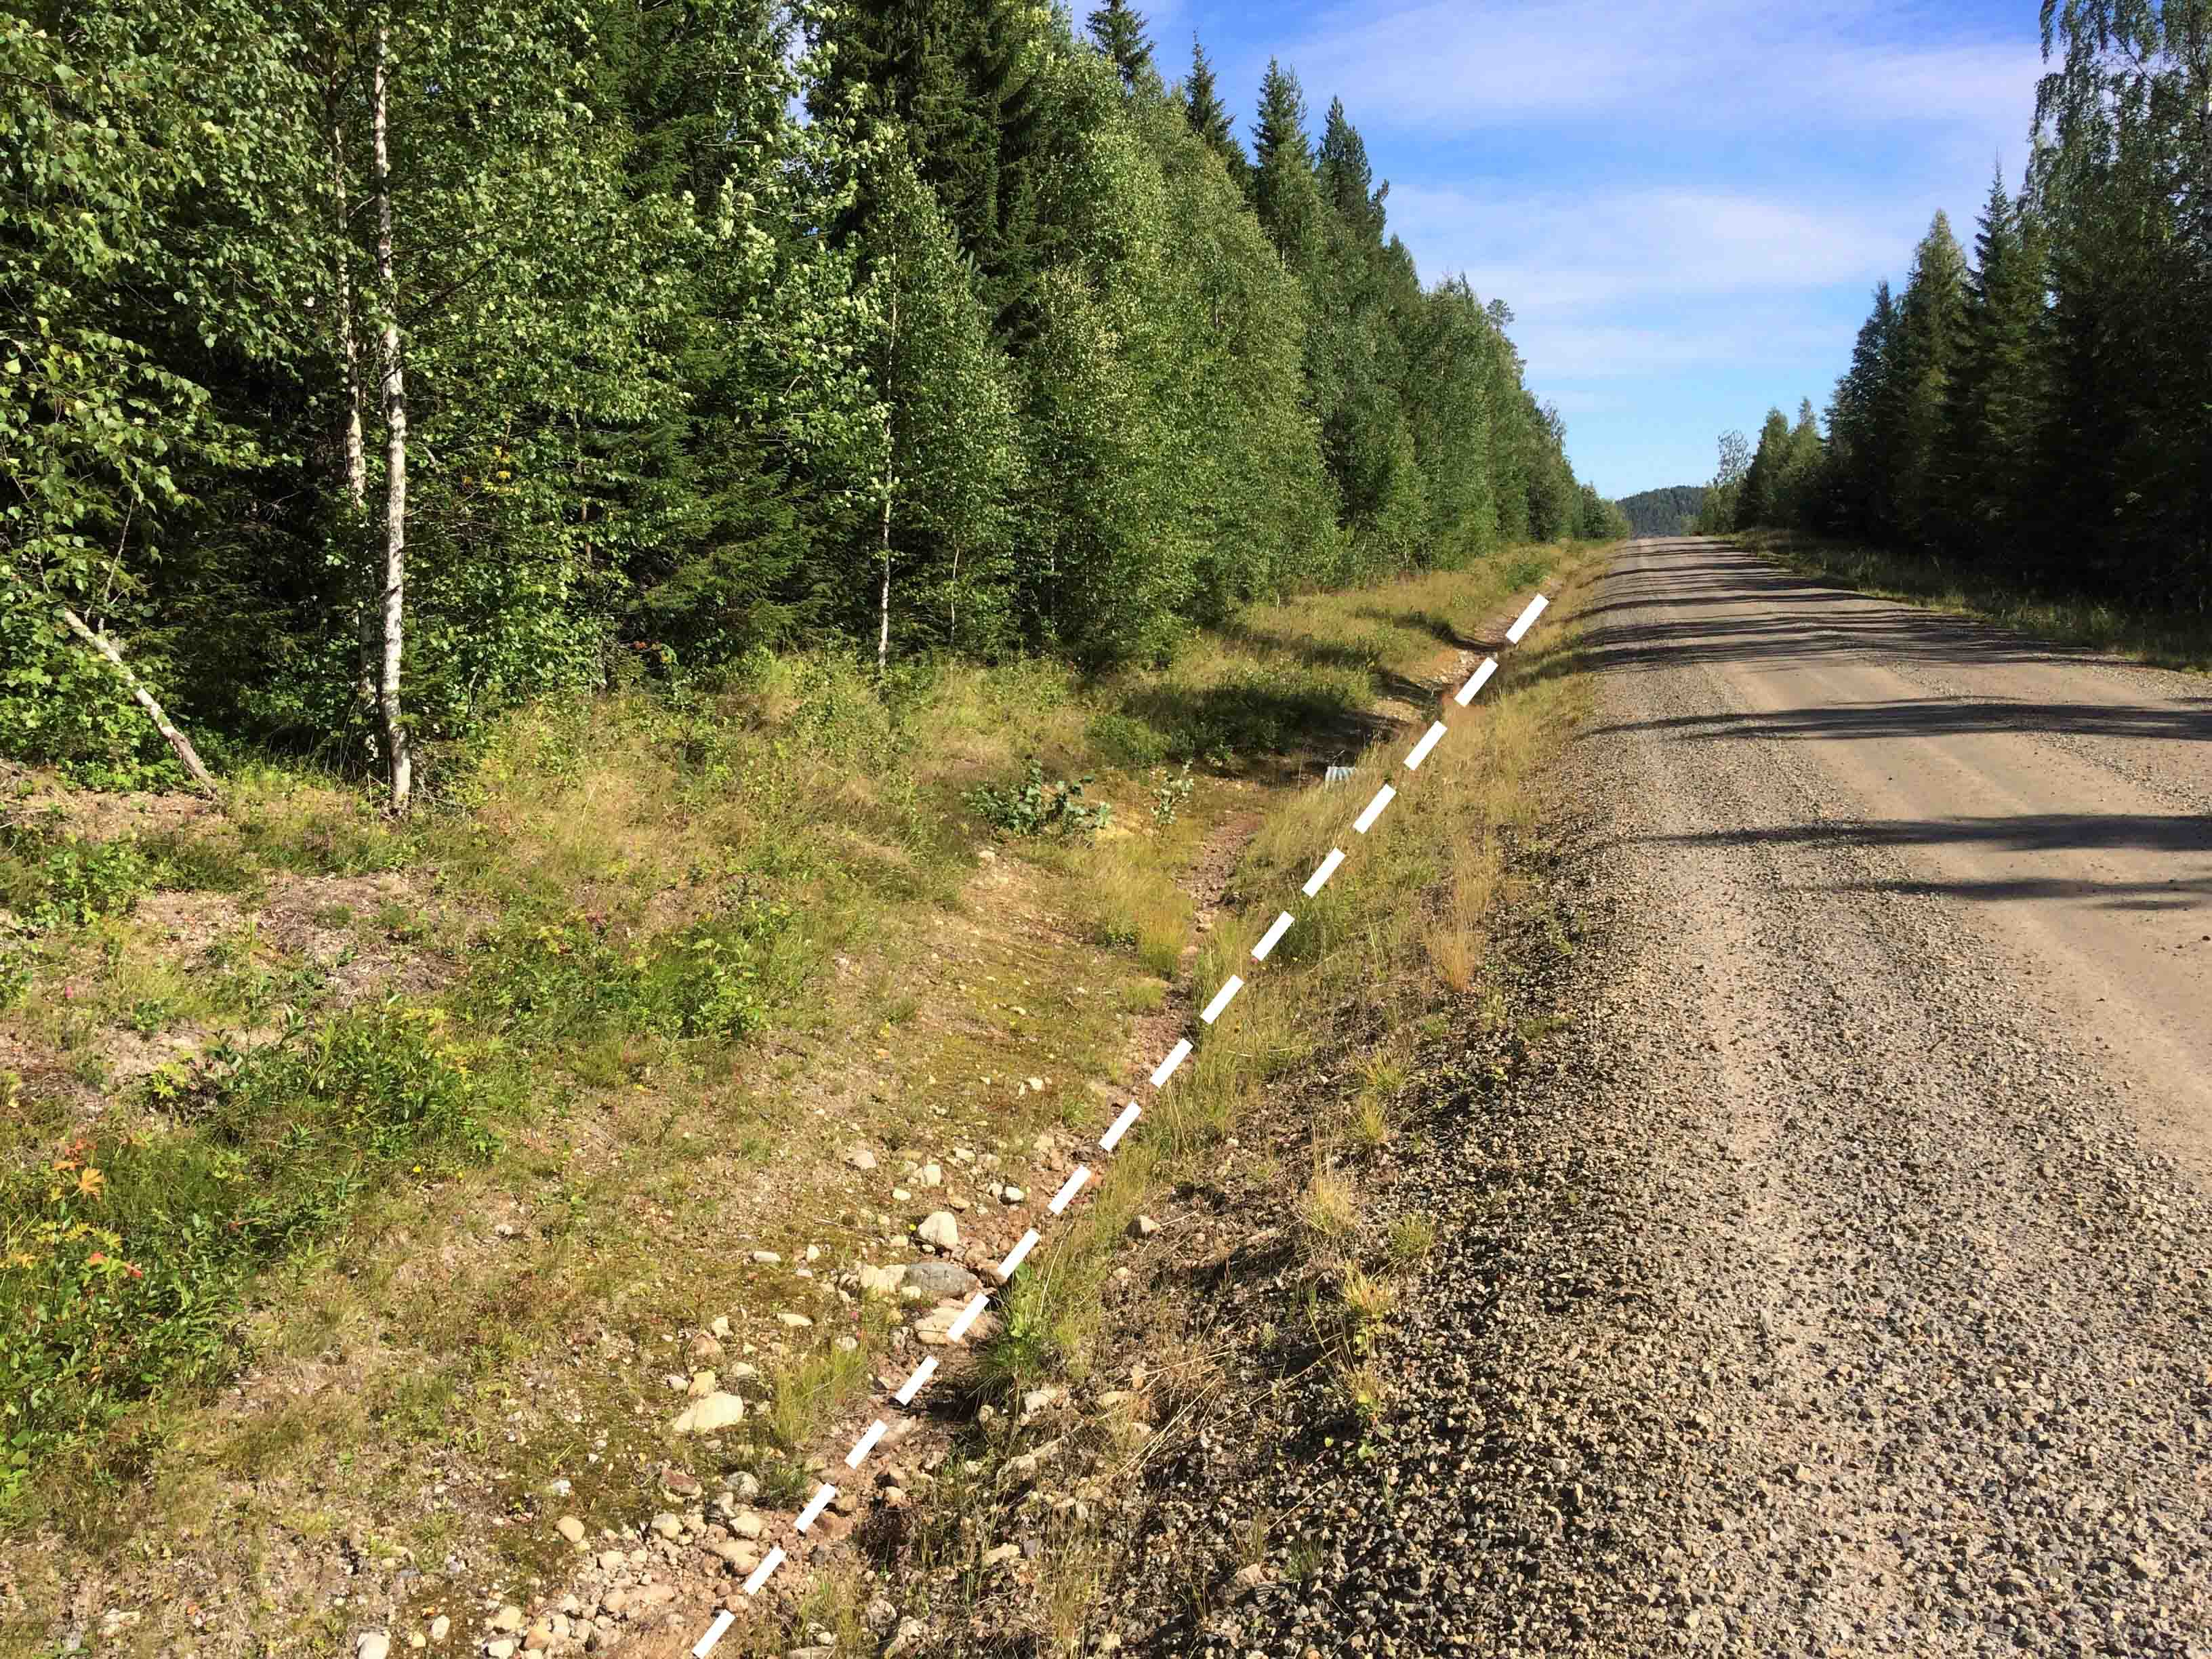
\includegraphics{./images/road_ditch_lo.jpg}}}\hspace{7pt}
    \subfigure[]{
        \resizebox*{6.85cm}{!}{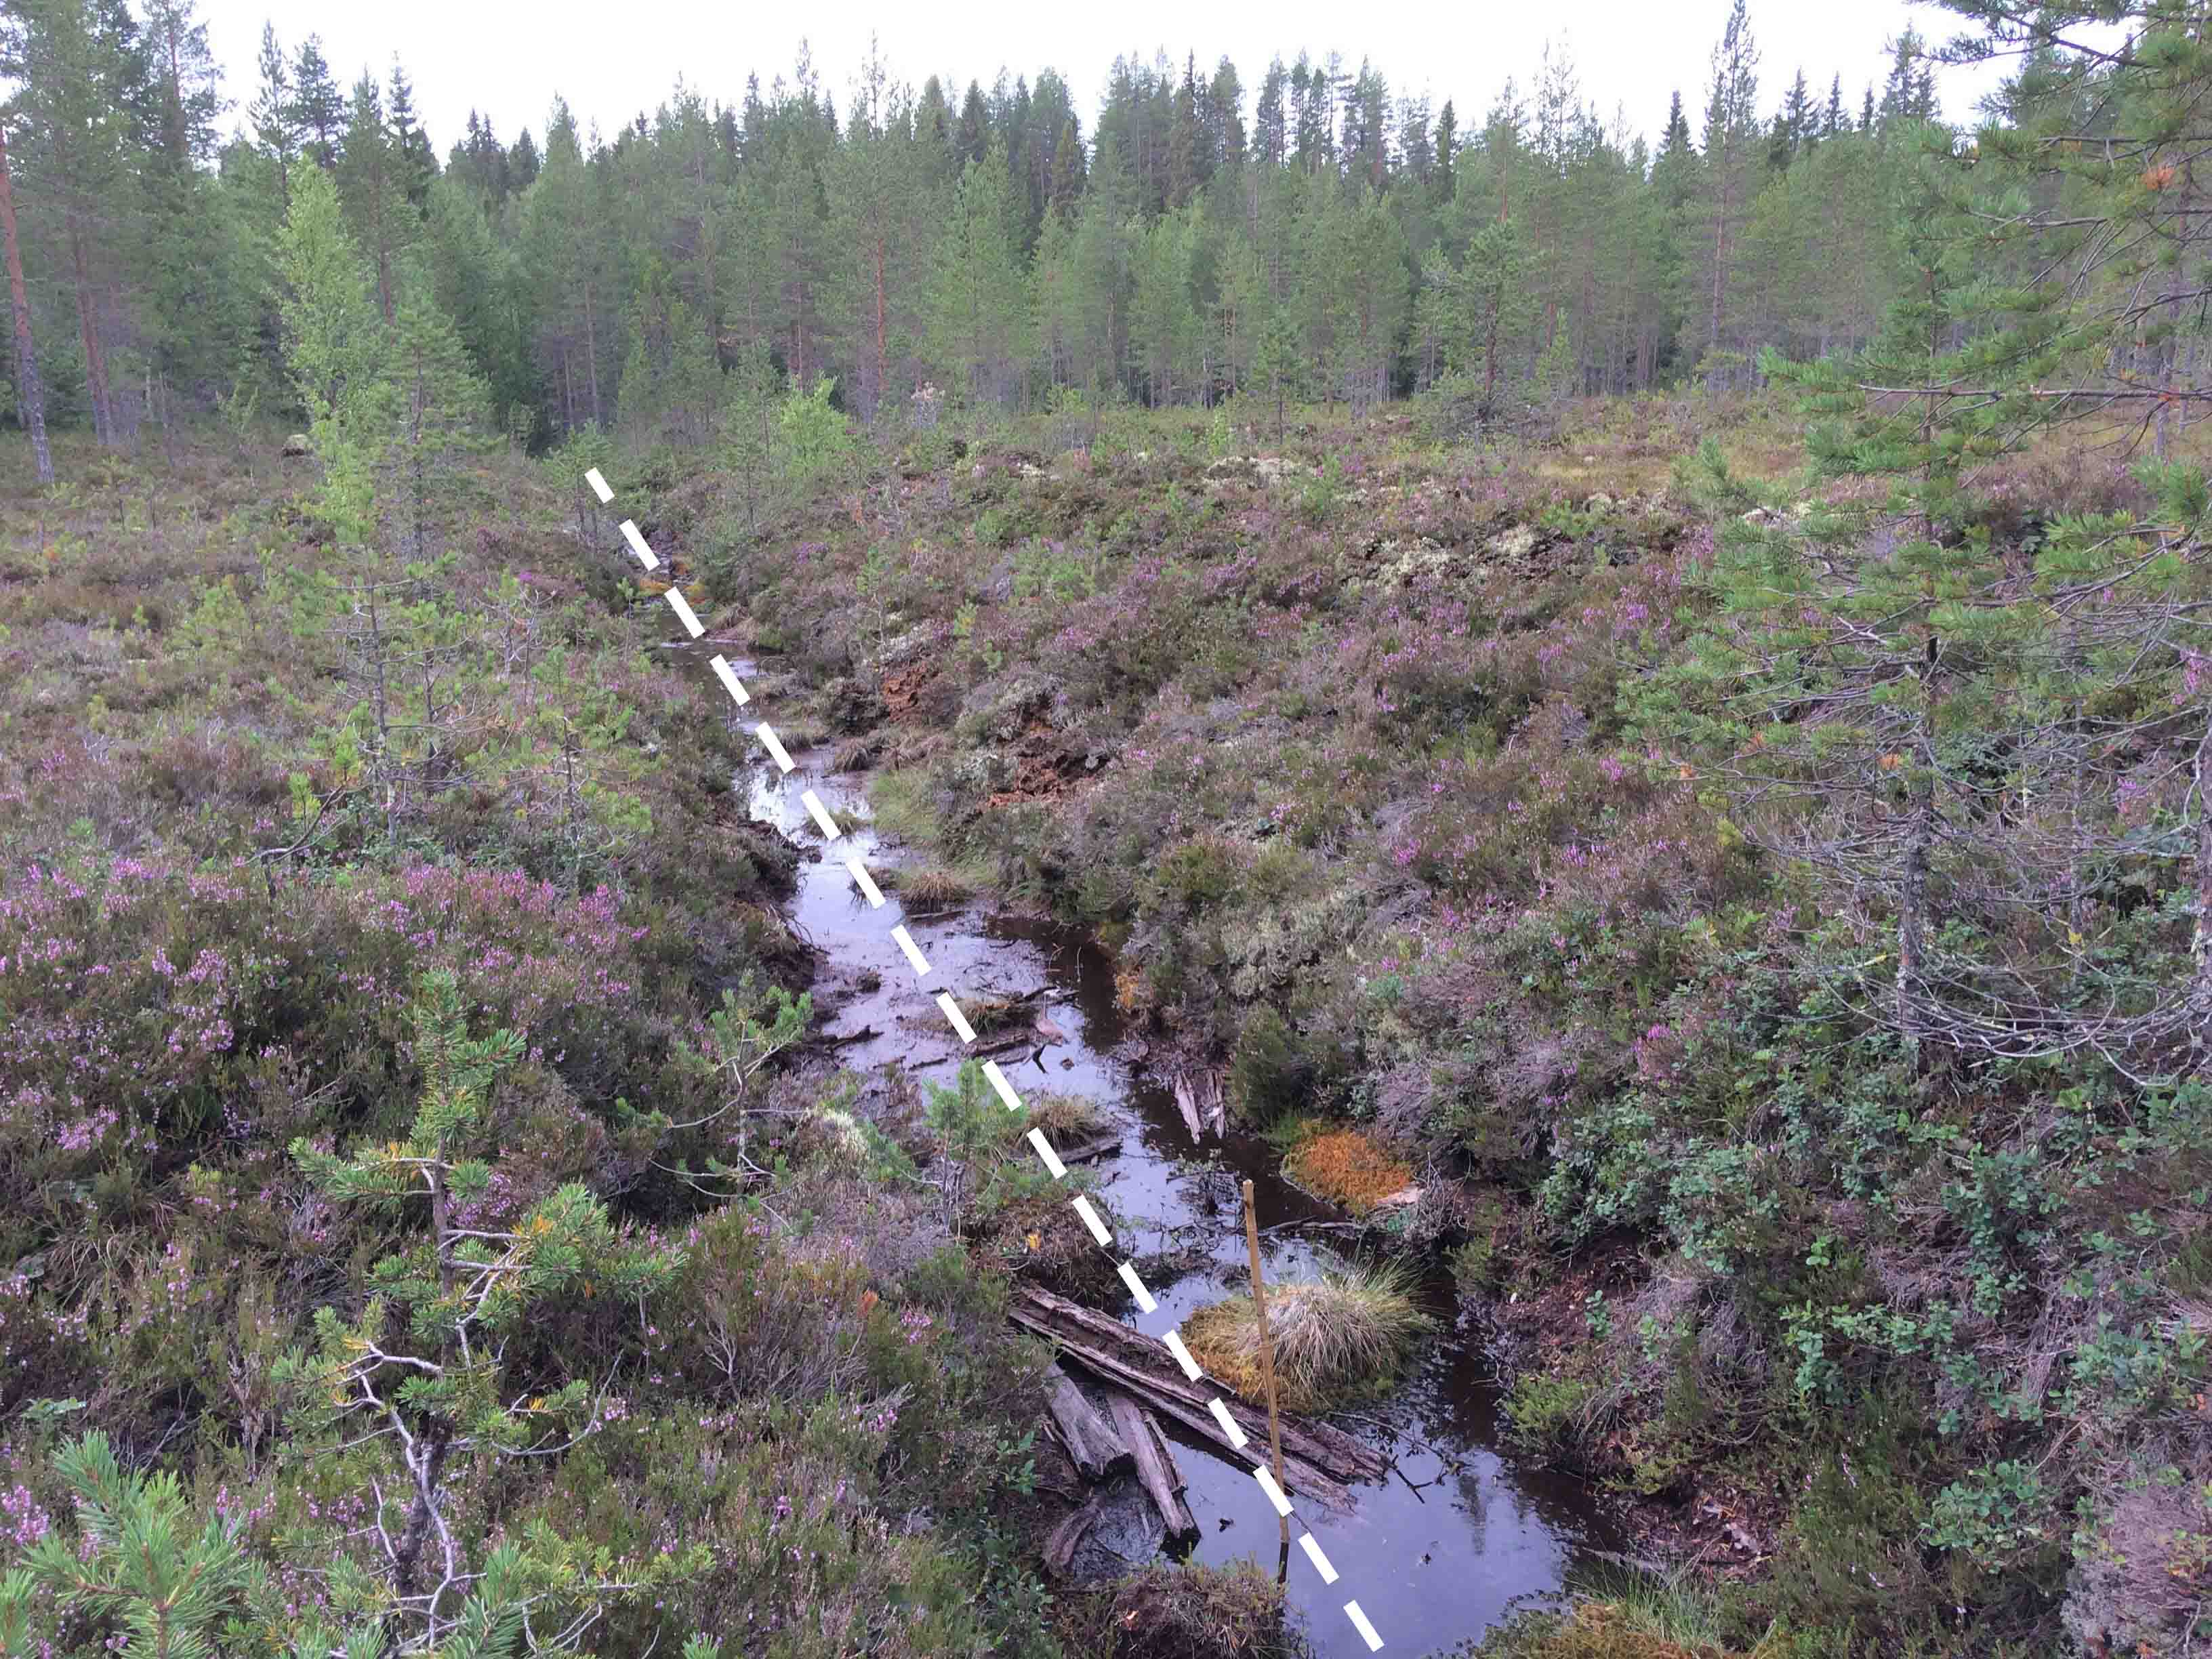
\includegraphics{./images/mire_ditch_lo.jpg}}}
    \subfigure[]{
        \resizebox*{6.85cm}{!}{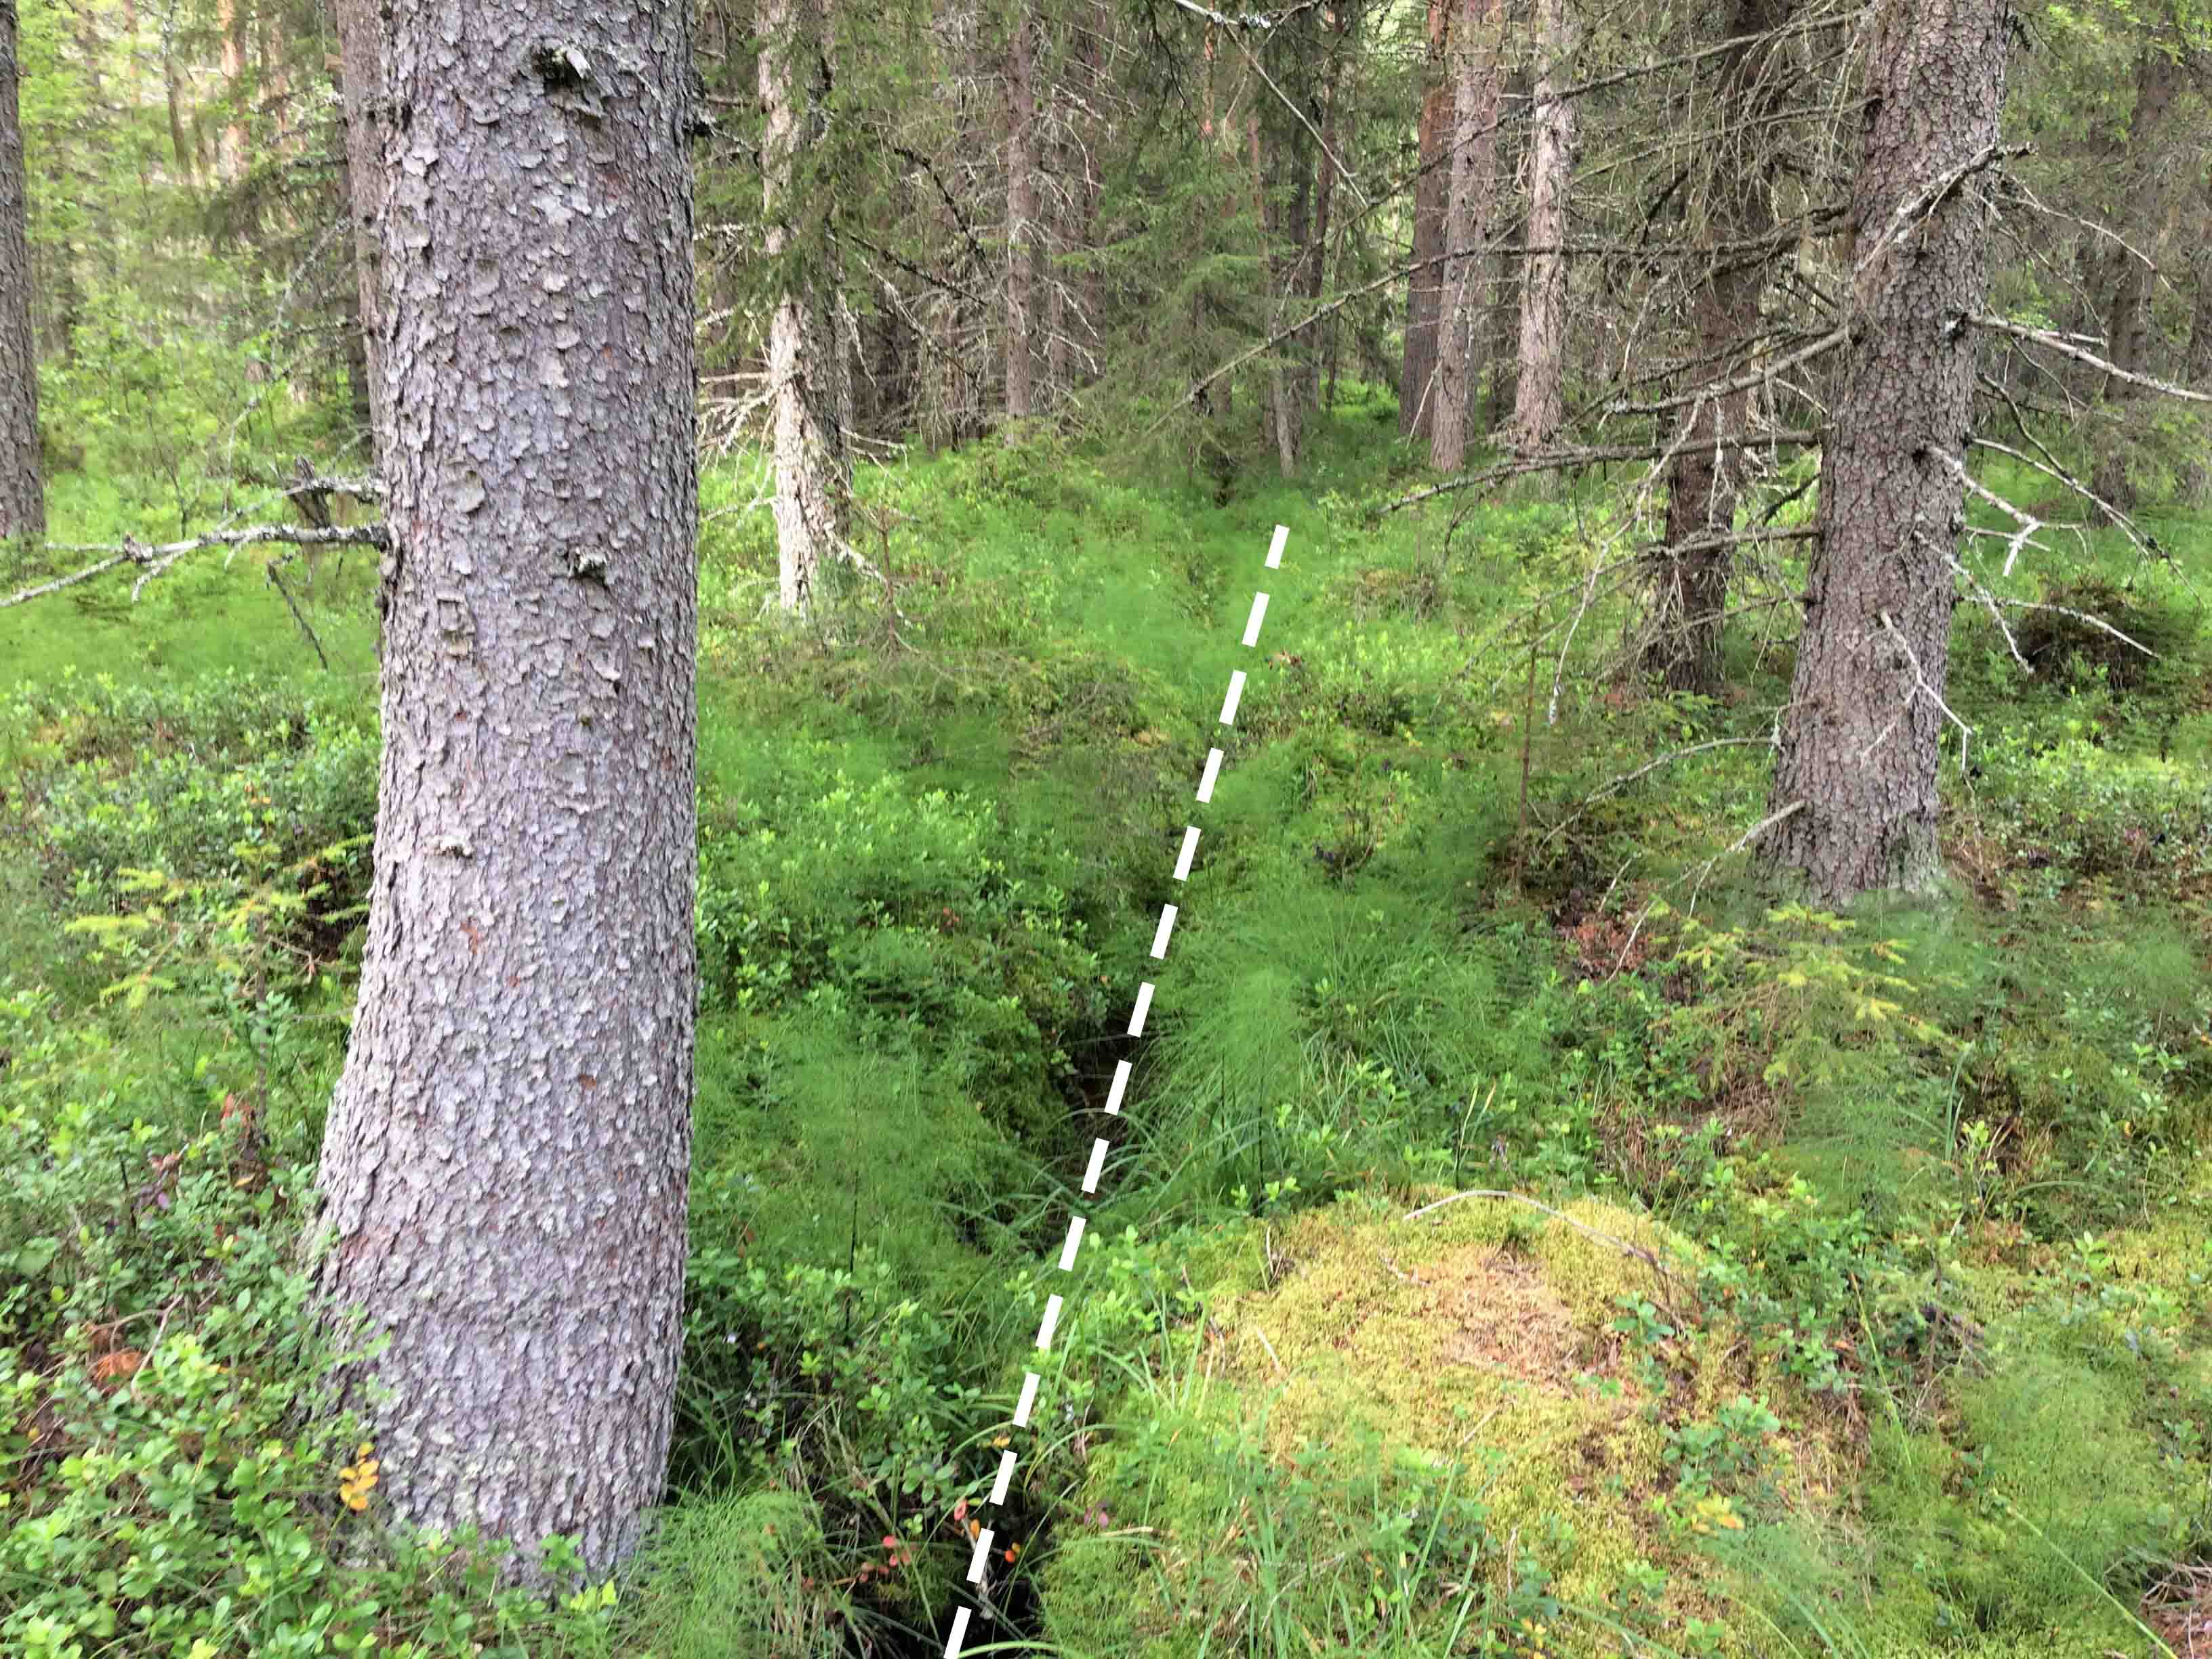
\includegraphics{./images/forest_ditch_lo.jpg}}}\hspace{7pt}
    \subfigure[]{
        \resizebox*{6.85cm}{!}{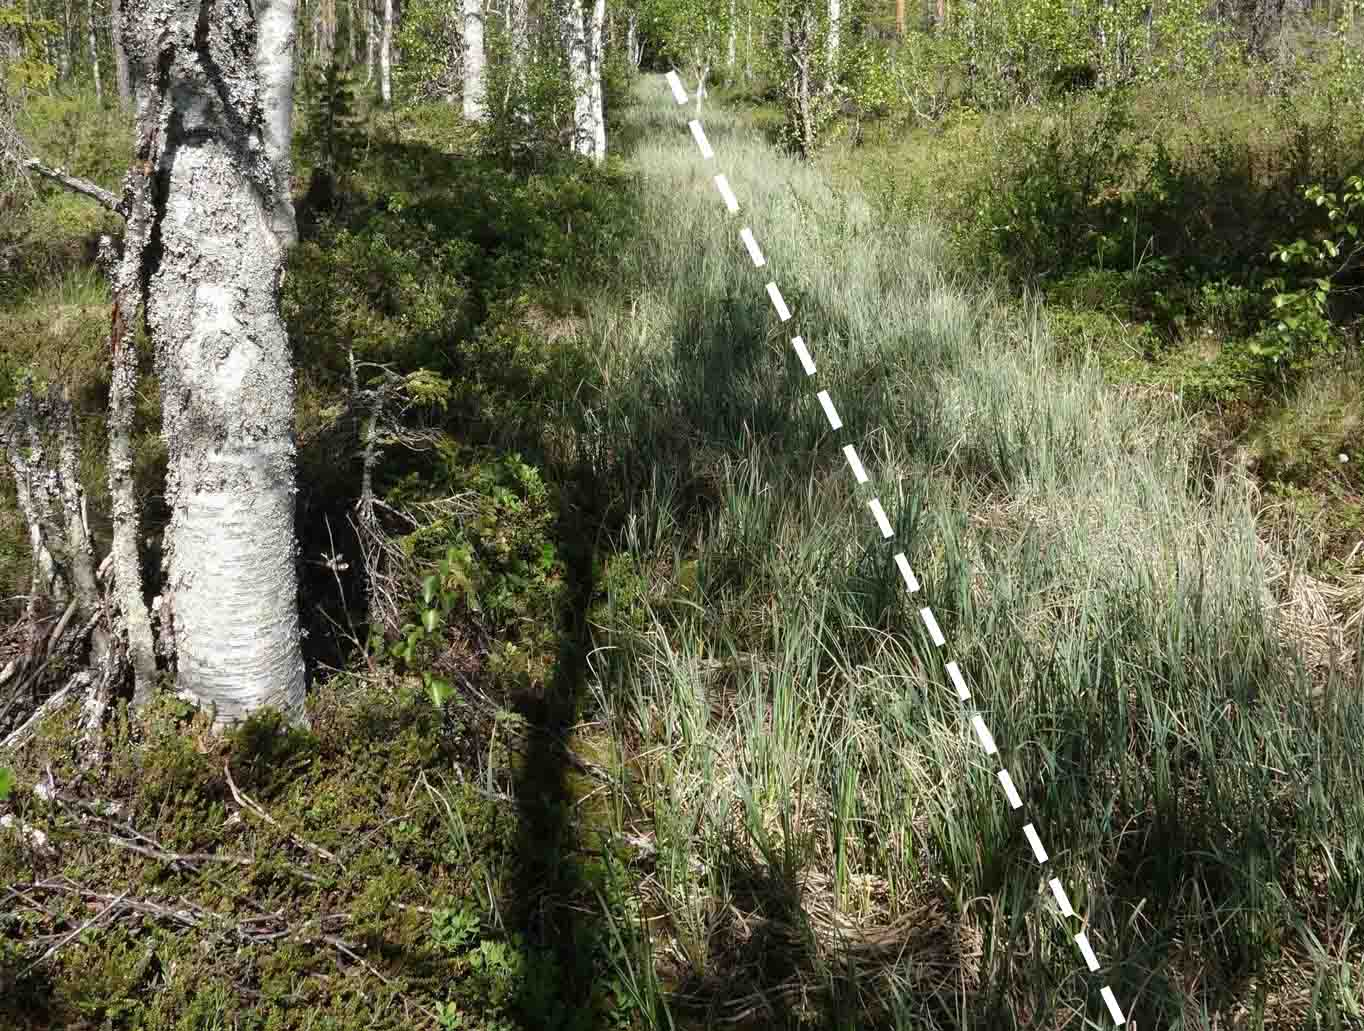
\includegraphics{./images/overgrown_ditch_lo.jpg}}}
    \caption{All photos show ditches in the study catchment. They illustrate the difficulty of capturing the ditches based on their form (i.e. an elongated, narrow, hollow in the ground). \textbf{a: }A roadside ditch. These are generally easily detected as they are usually found in open areas along the roads, and have often been maintained. \textbf{b: }A ditch in a mire; this is still easily detected, as there is no canopy and there is a clear elevation difference between the ditch and surrounding area. \textbf{c: }A narrow, more or less  overgrown ditch in a dense forest stand. \textbf{d: }A ditch in a mire that has more or less grown back in with \textit{Sphagnum sp.} and \textit{Carex}, likely also in combination with subsiding surrounding soils. Such ditches can be found in the field as the vegetation differs, but as there is no longer an elevation difference between the ditch and the surrounding soils it will not be detected in the DEM. Photos a-c: E. Maher Hasselquist  Photo d: G. Norstedt}
    \label{fig:ditchpictures}
\end{figure}

Hypothetically, it should be quite easy to detect ditches using LiDAR data. In practice, however, there are many variables affecting the results, such as the point density and the interpolation method used to create the DEM. \citet{rapinel} found that the results were usually more sensitive to the point density (ranging 1-4 points $m^{2}$ in their study) than the interpolation method. They retrieved 54.8 and 63.8 \% of the ditches on the Acuey and Boucey marches in France, compared to 70.28 \% in our study. However, in our study we had a point density of 20 points $m^{2}$, so the quality of the DEM in our study ought to be robust, which may have contributed to our higher retrieval rate. \hyperref[fig:resultstreesbushes]{Figure} \ref{fig:resultstreesbushes} \hyperref[fig:resultstreesbushes]{(a, b)} illustrates the difference in the quality of the LiDAR data where the laser pulses have caught in trees or shrubs. When too few LiDAR points reach the ground, the DEM generation is forced to interpolate over a larger area, leading to inaccuracies in the ground DEM.

\begin{figure} [!htb]
    \centering
    \subfigure[]{
        \resizebox*{6.8cm}{!}{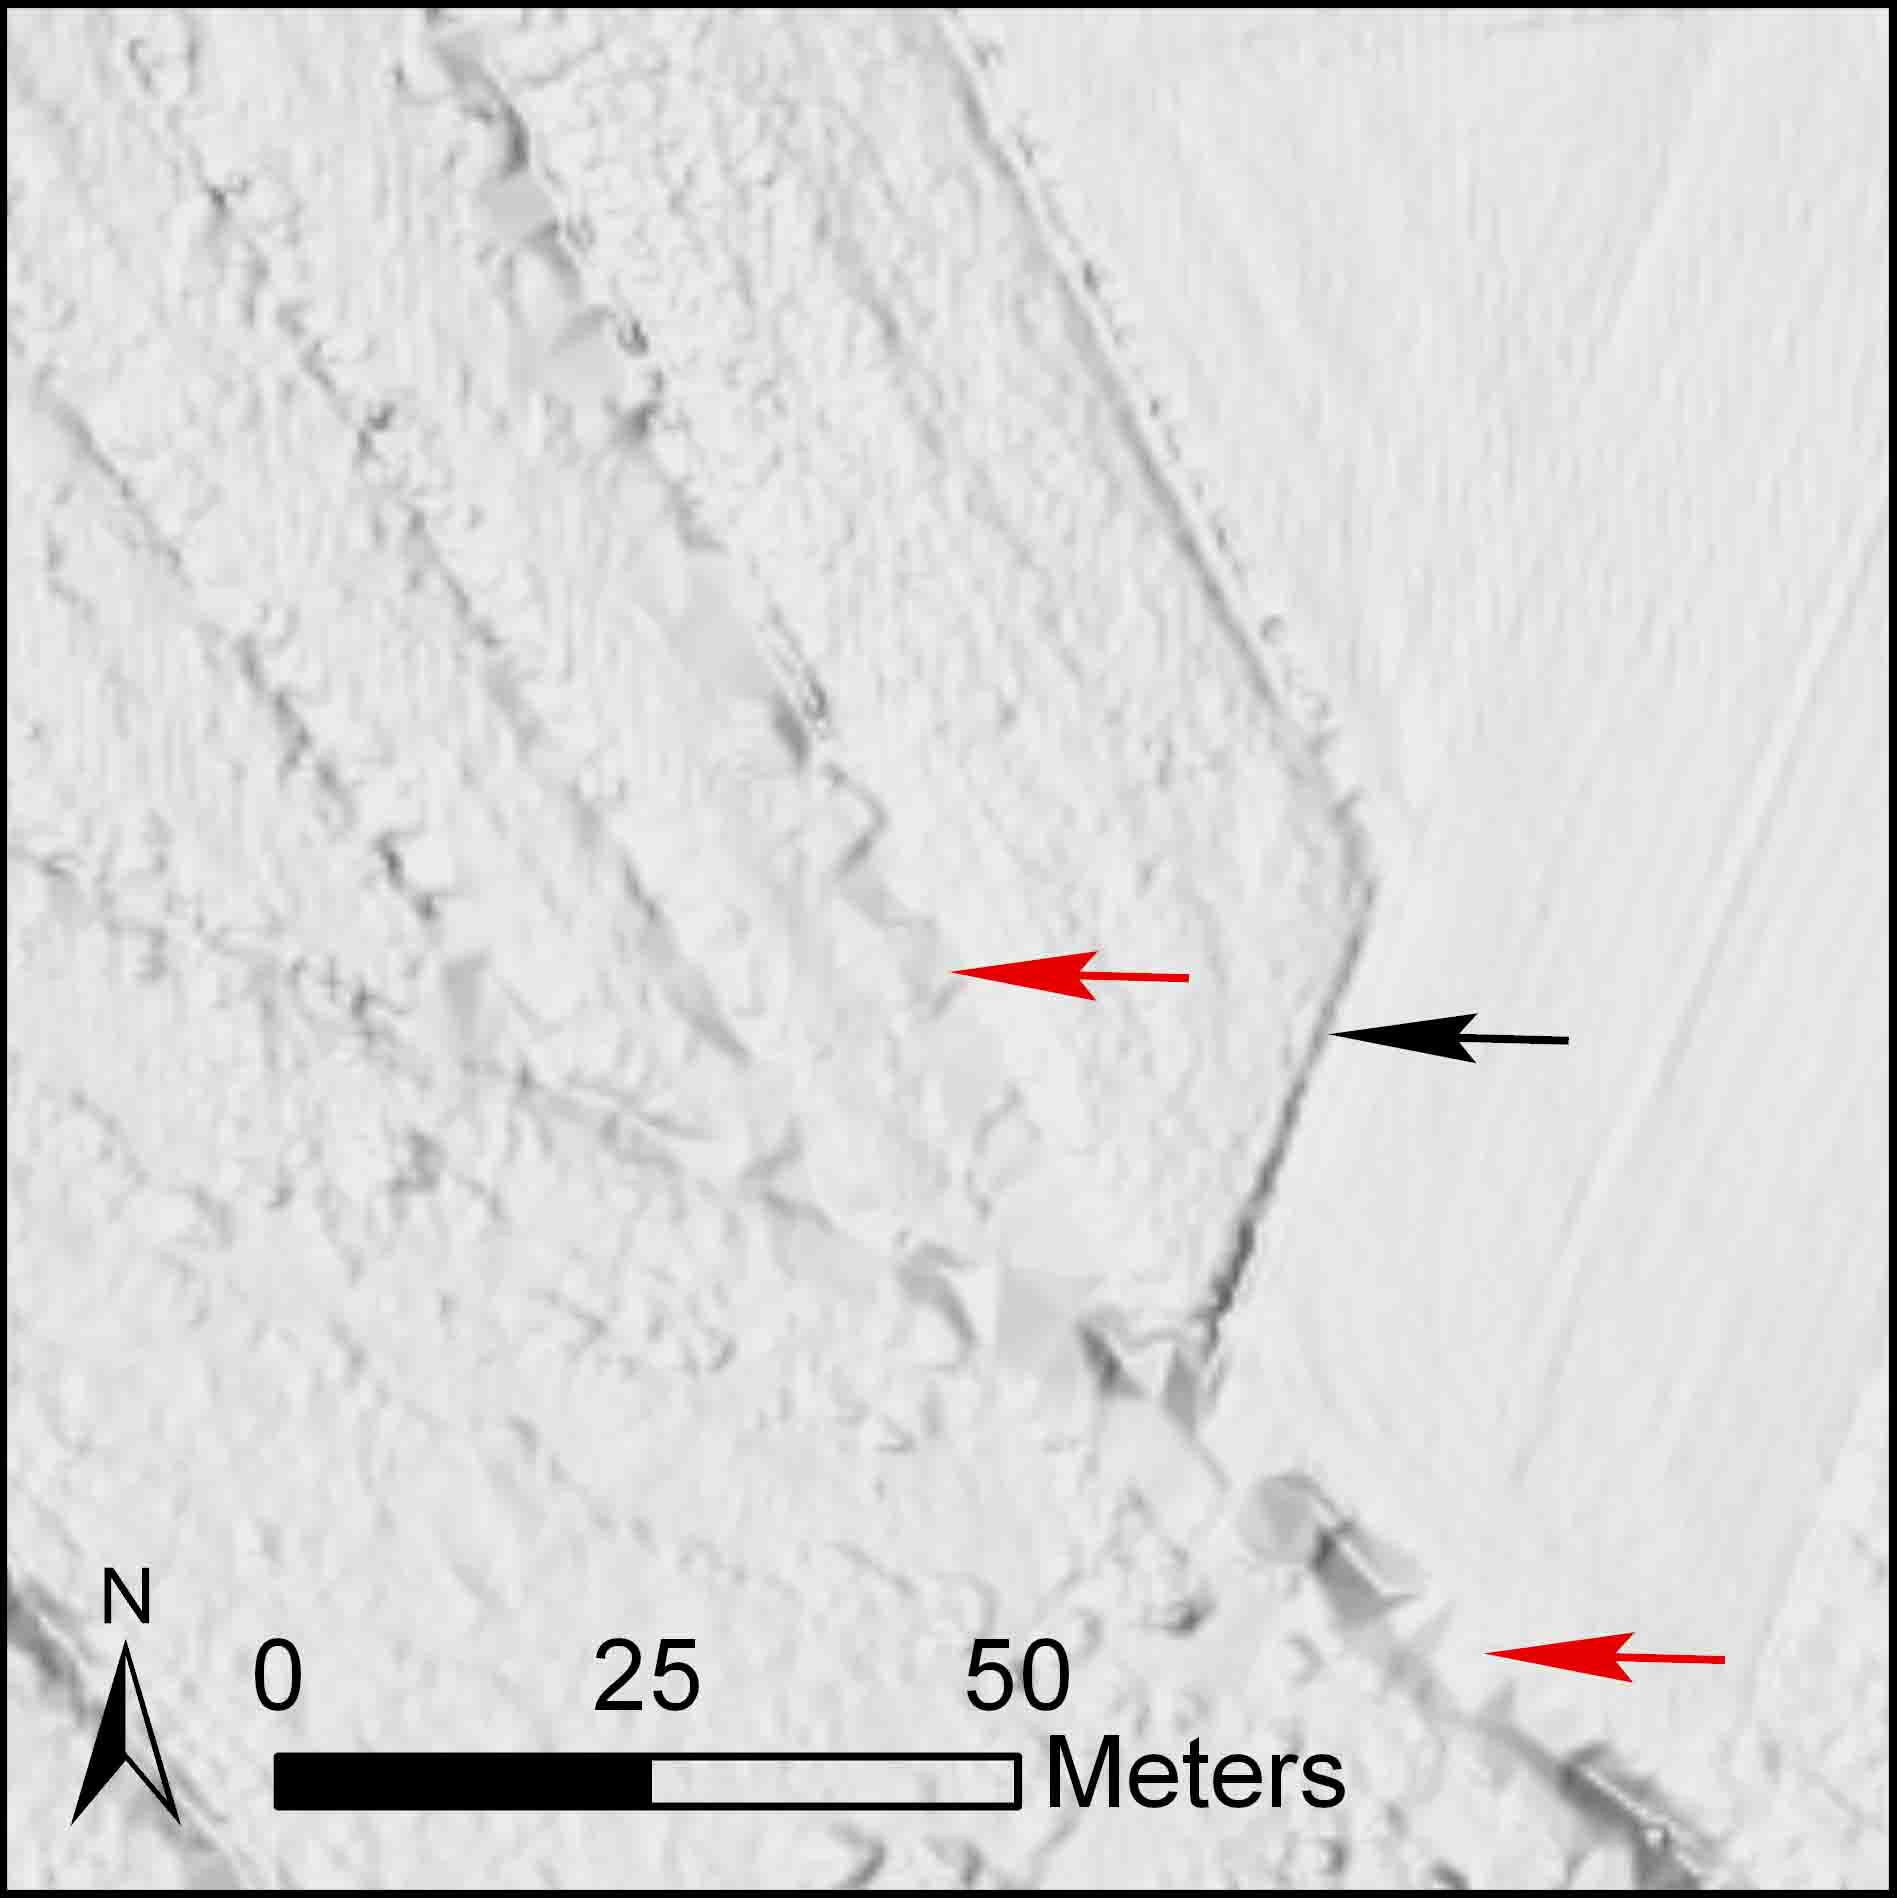
\includegraphics{./images/results_trees_bushes_1_lo.jpg}}}\hspace{7pt}
    \subfigure[]{
        \resizebox*{6.8cm}{!}{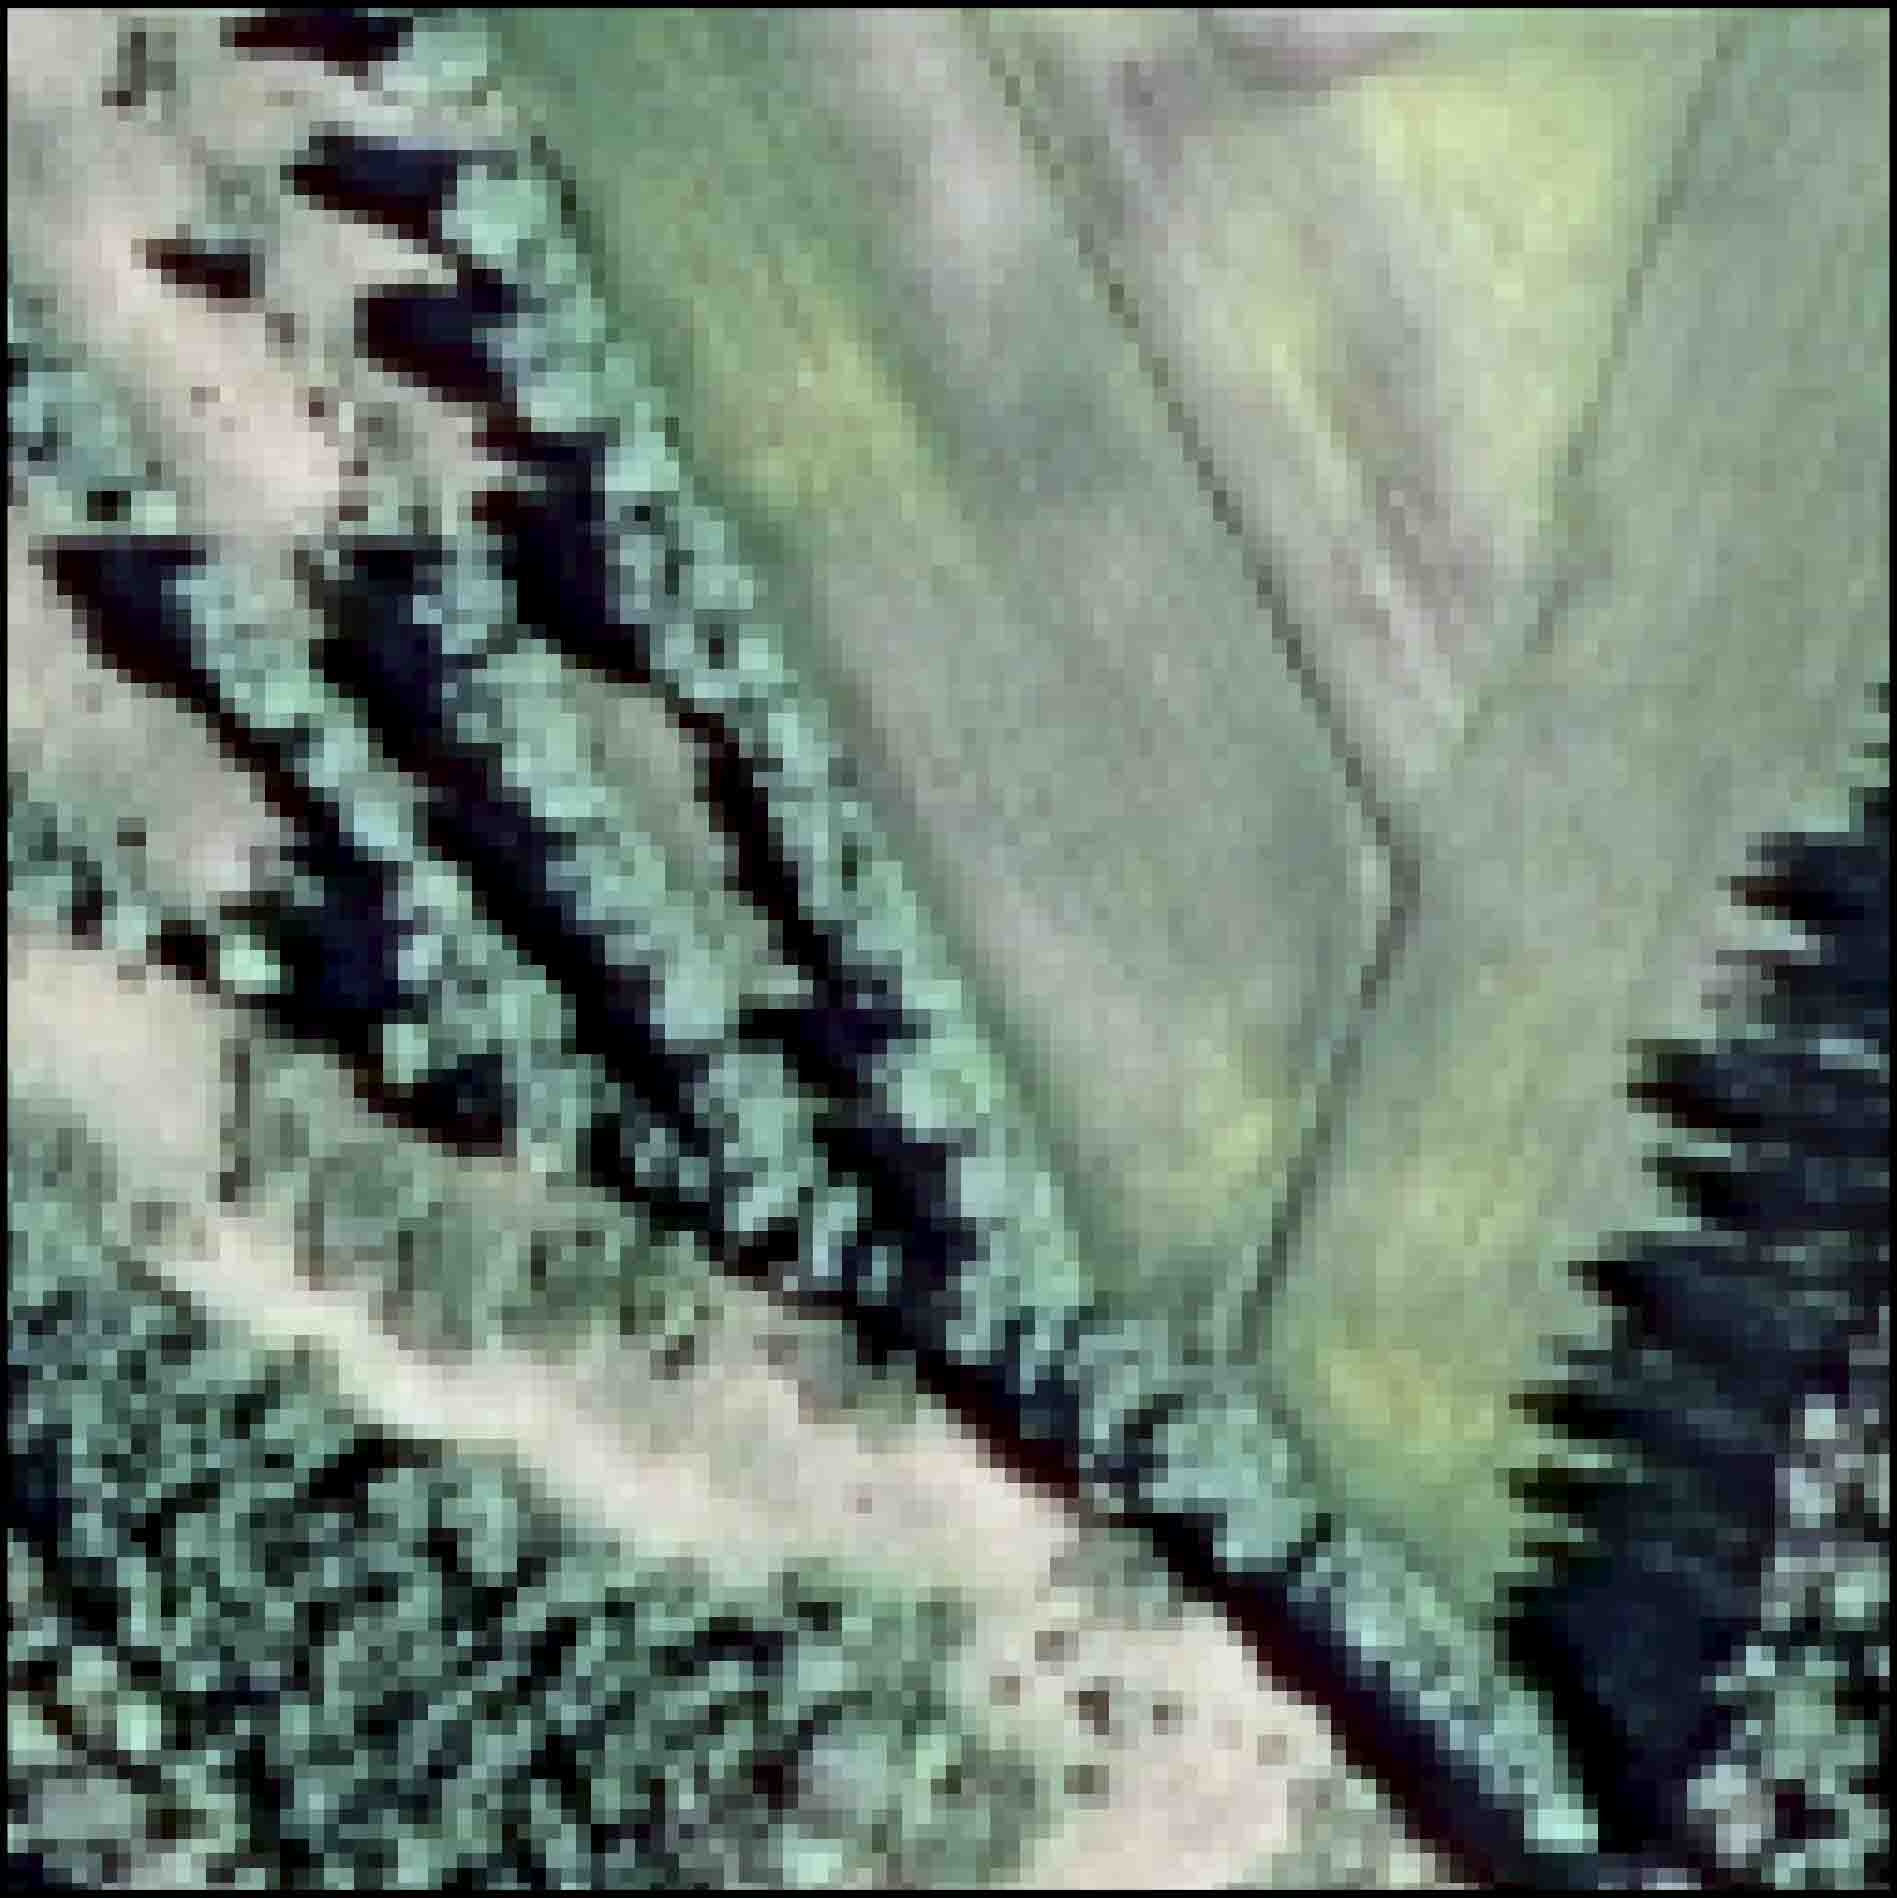
\includegraphics{./images/results_trees_bushes_2_lo.jpg}}}
    \subfigure[]{
        \resizebox*{6.8cm}{!}{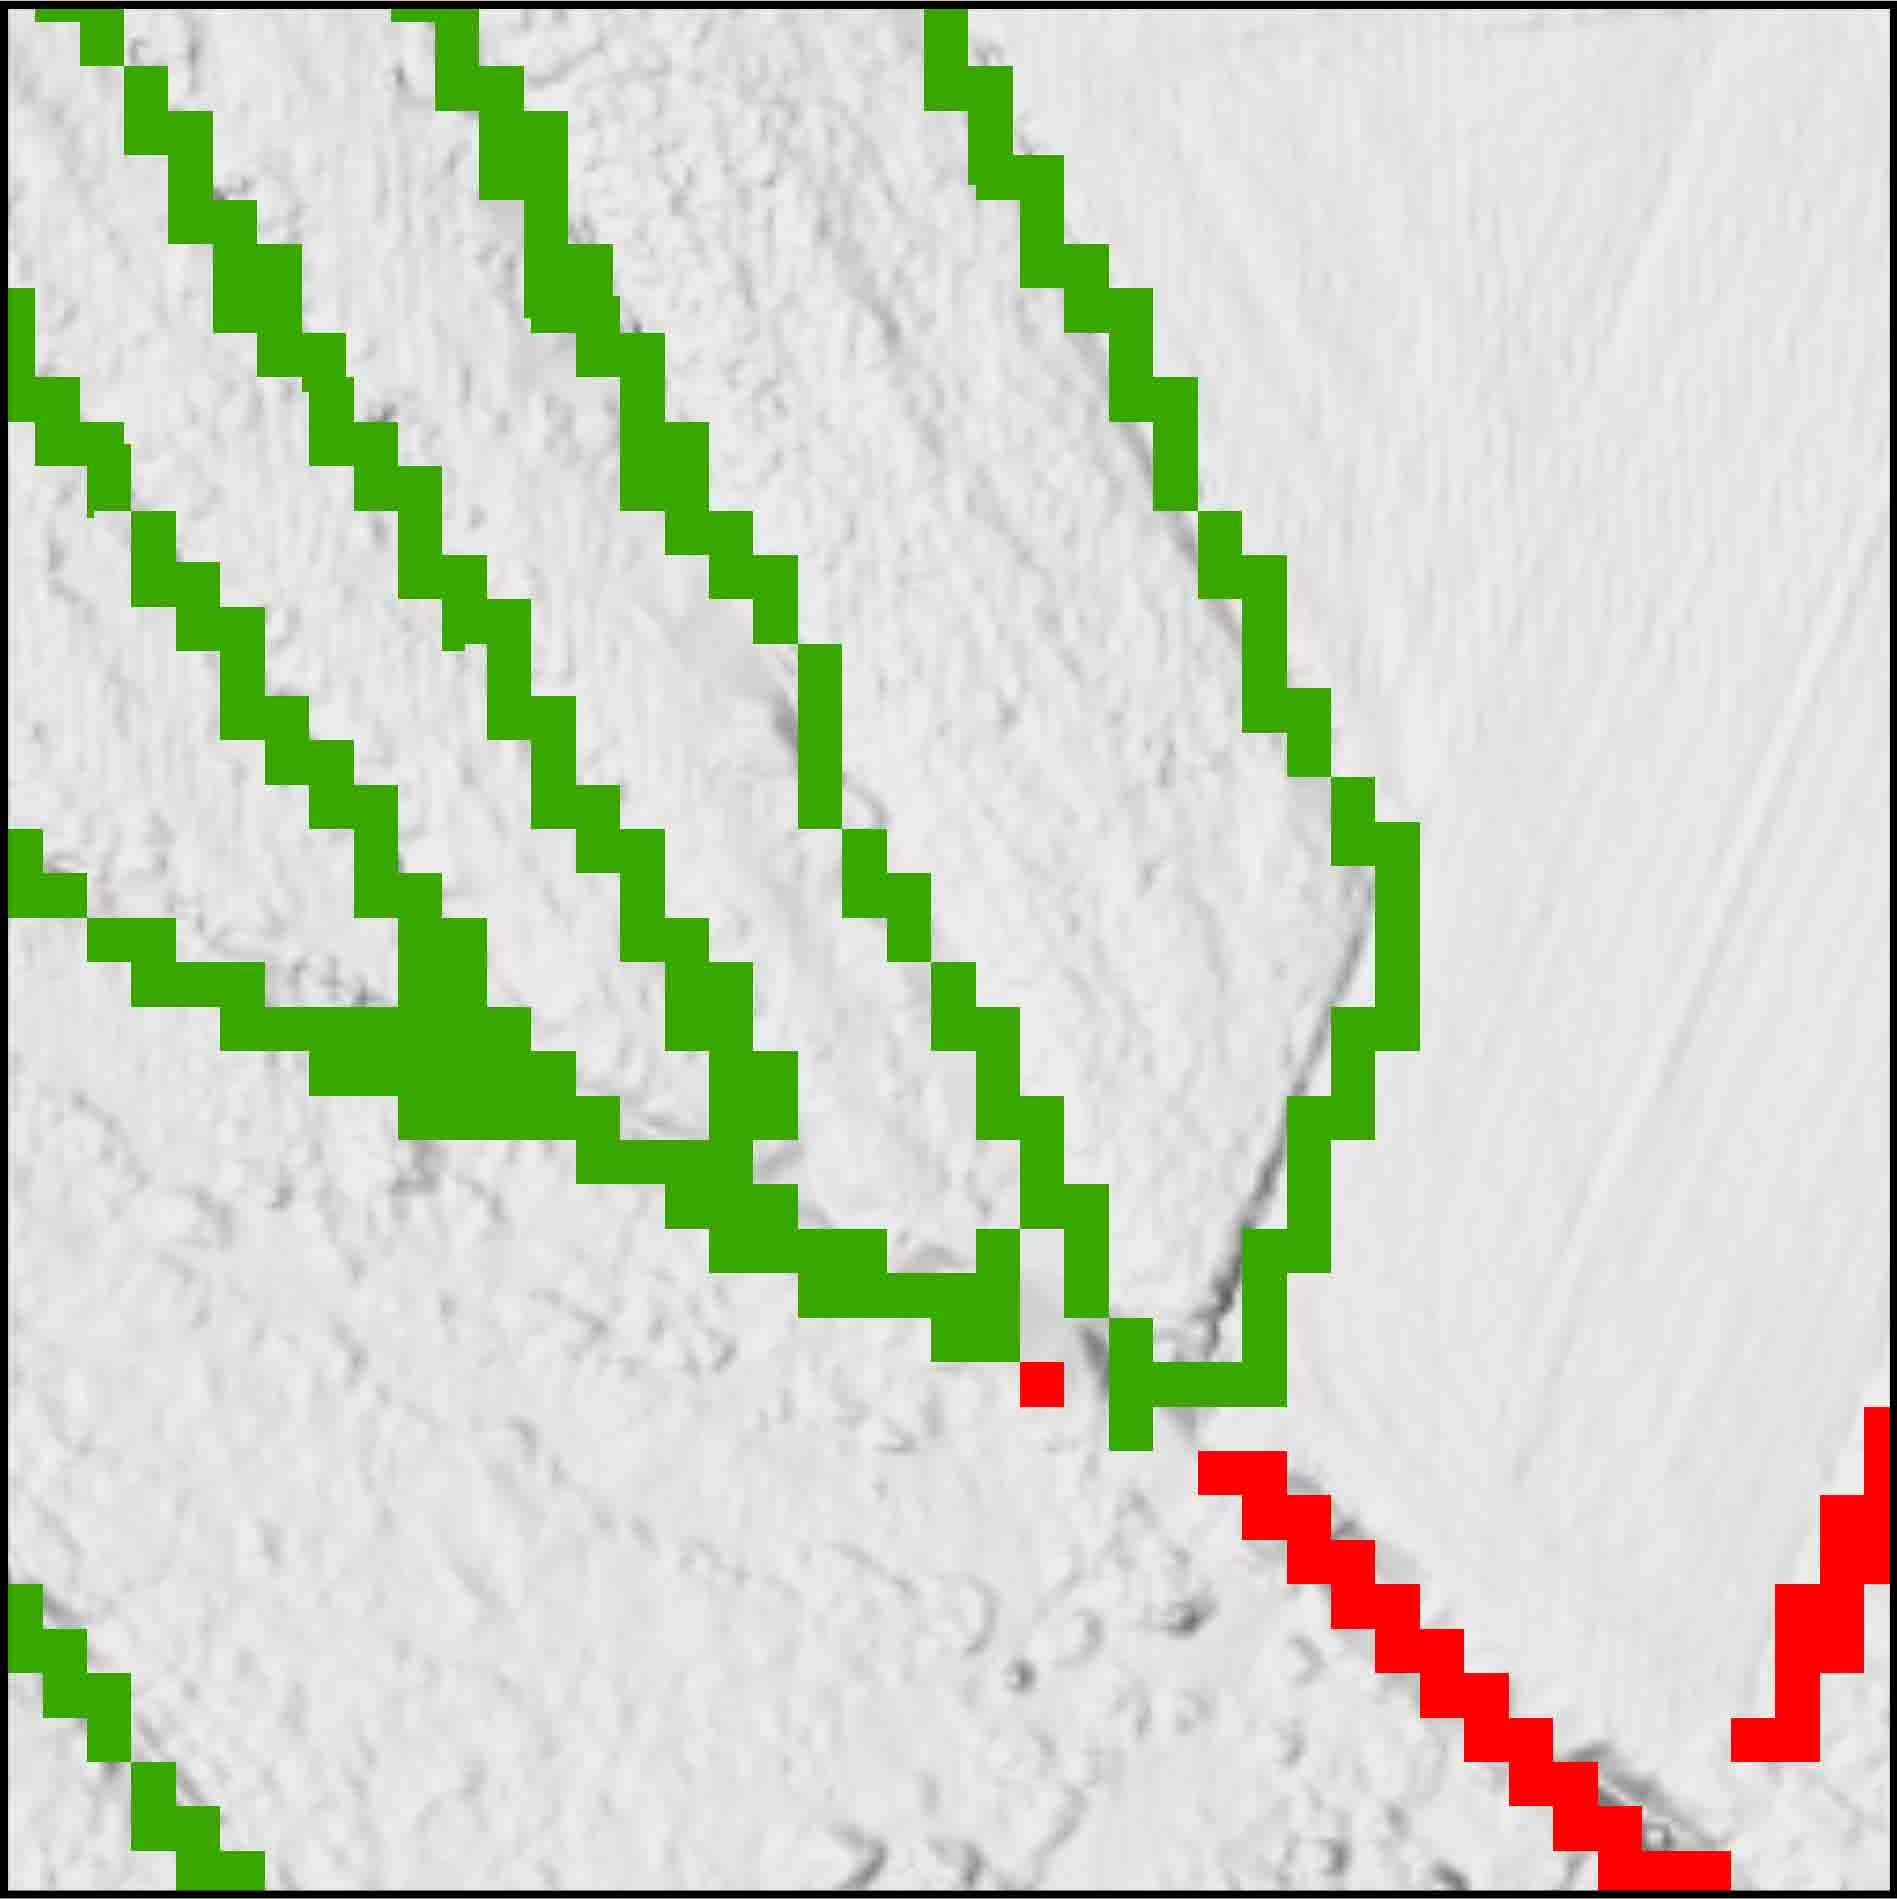
\includegraphics{./images/results_trees_bushes_3_lo.jpg}}}\hspace{7pt}
    \subfigure[]{
        \resizebox*{6.8cm}{!}{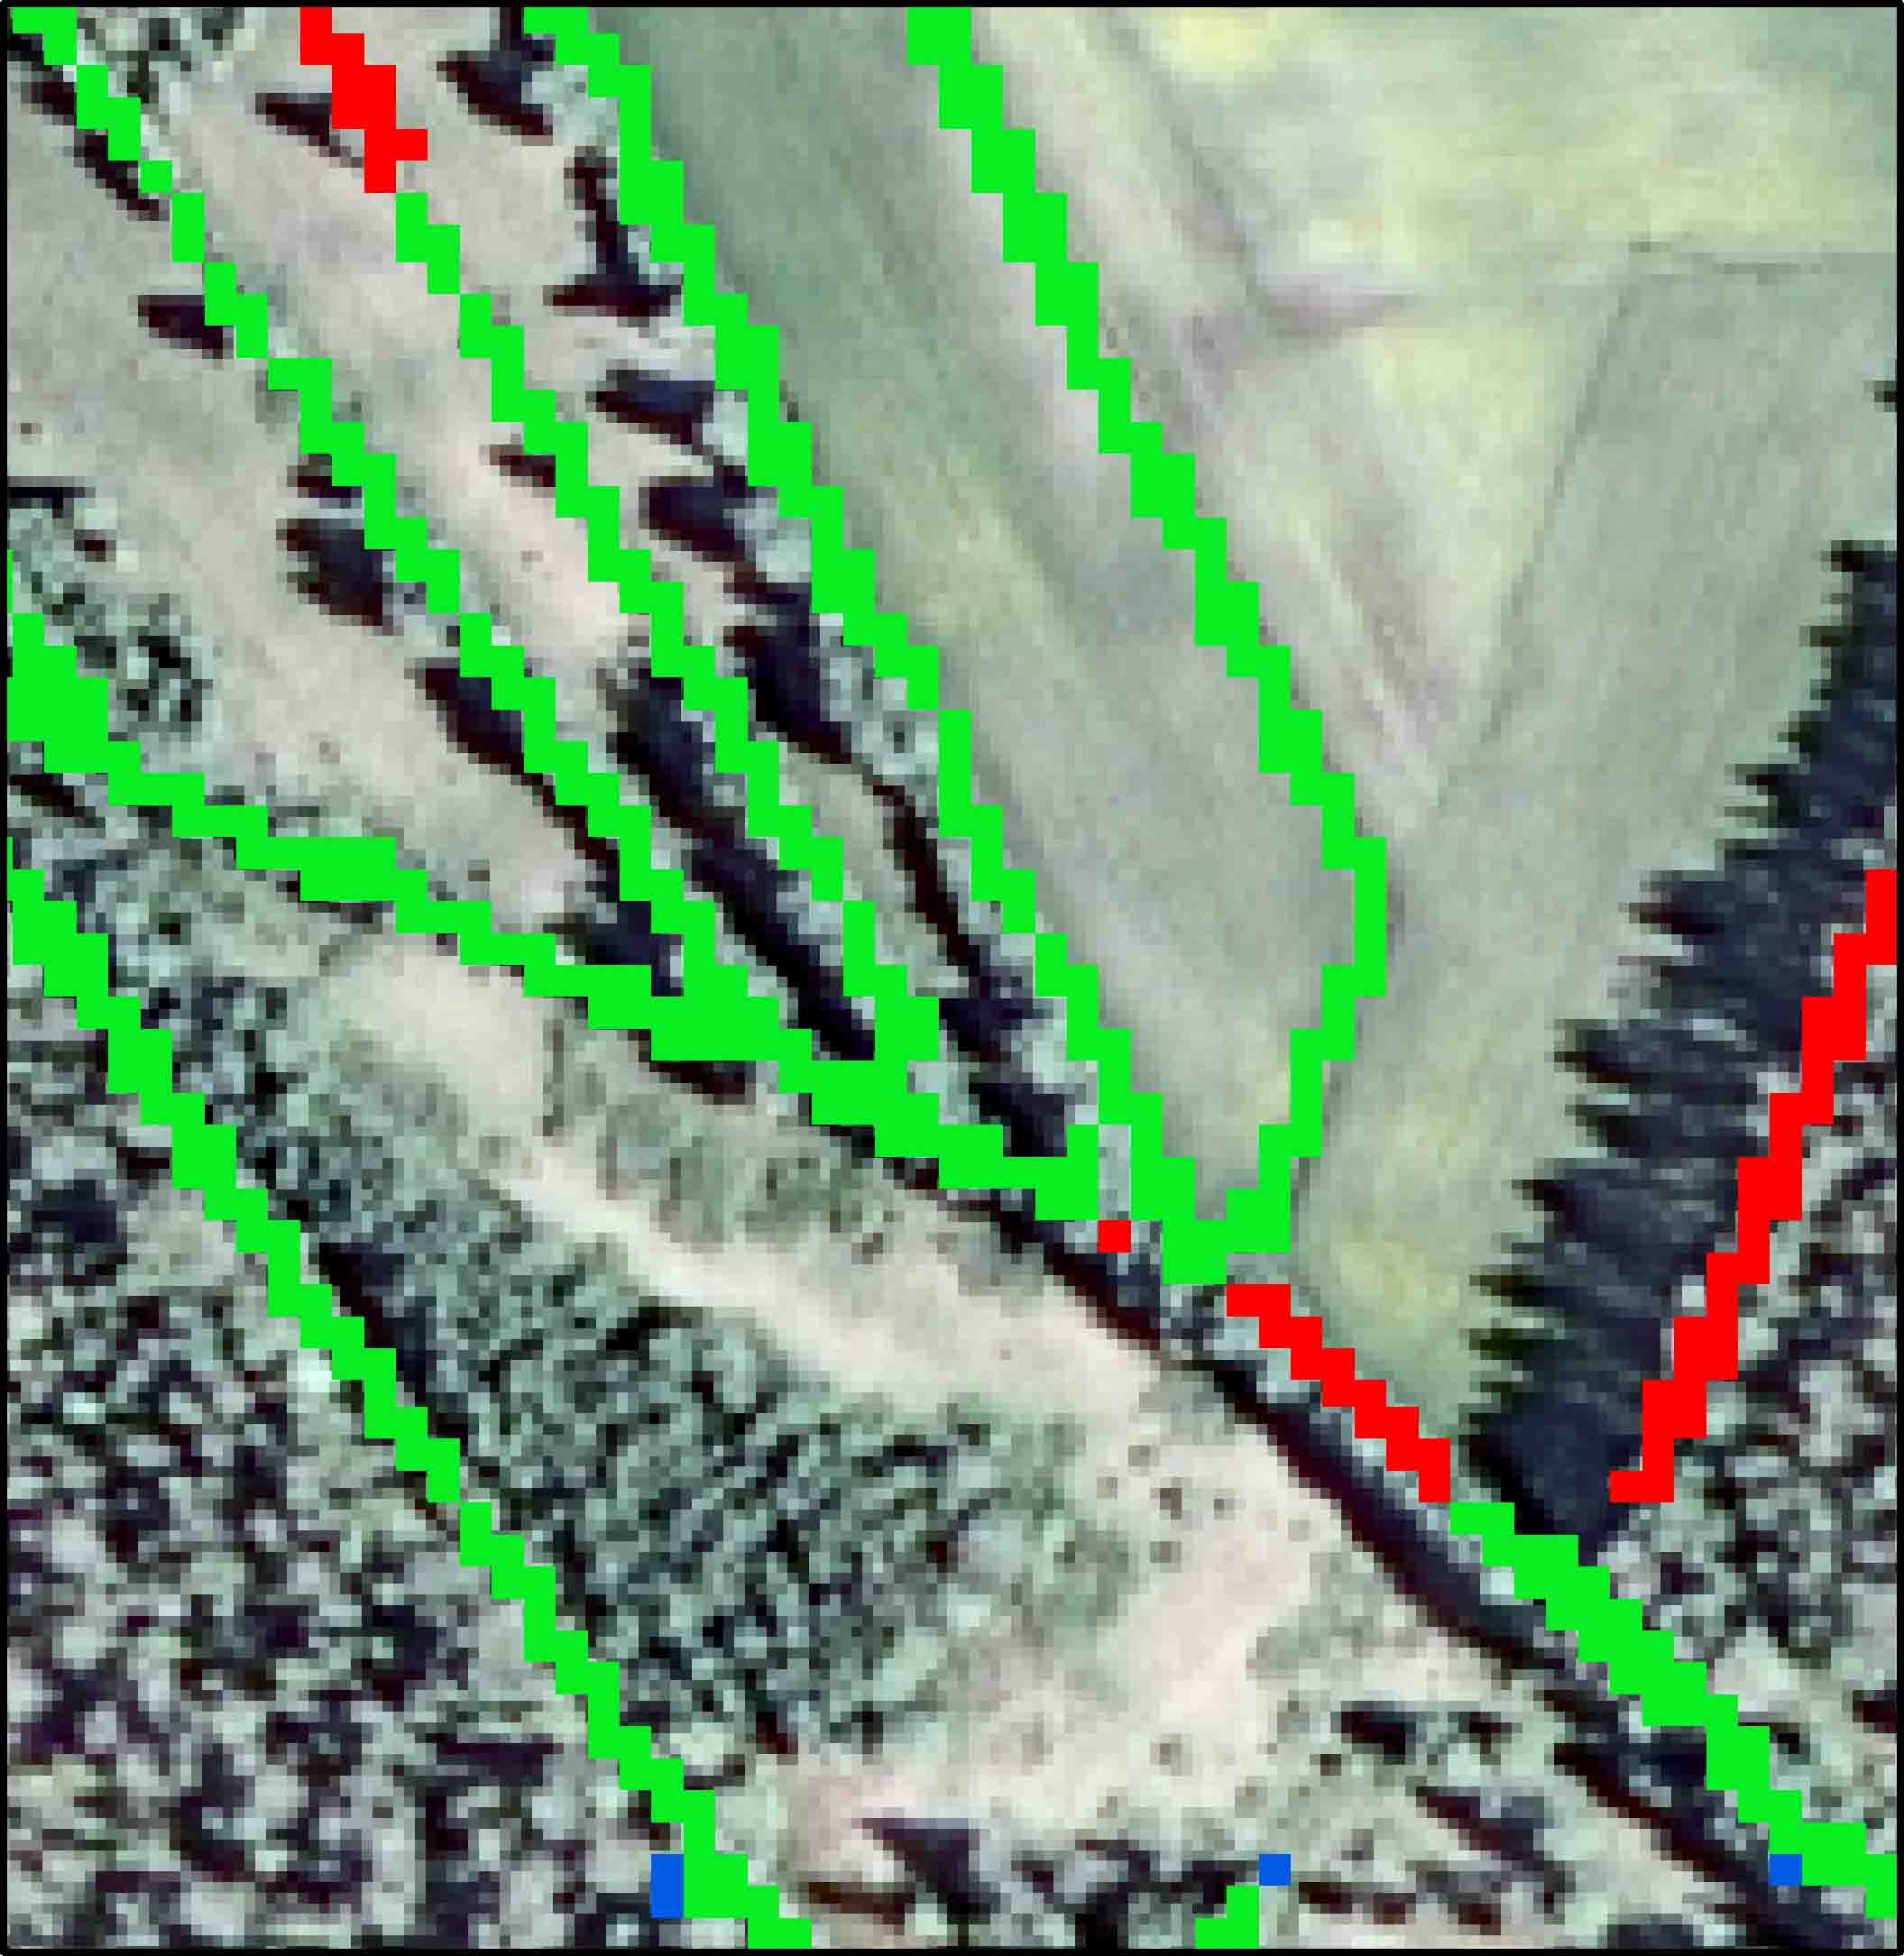
\includegraphics{./images/results_trees_bushes_4_lo.jpg}}}
    \caption{\textbf{a} and \textbf{b} illustrate that despite a point density of 20 points $m^2$, not all points reach the ground in places with dense vegetation. In \textbf{a} there is a clear difference between the smooth surface of the DEM in the open area (black arrow), and in the areas covered by trees and shrubs (red arrows), where the DEM is much coarser due to interpolation with a lower number of LiDAR points here. The orthophoto (\textbf{b}), clearly shows that trees and shrubs are growing in the ditches in this area. This makes it more difficult to detect ditches. However, despite these coarser grid points in the DEM, \textbf{c} and \textbf{d} shows that the ditch detector still managed to capture a majority of the ditches (green), and only failed at certain points (red).}
    \label{fig:resultstreesbushes}
\end{figure}

With our method, natural streams were often classified as false positives (\hyperref[fig:resultsillustrations]{Figure} \ref{fig:resultsillustrations} \hyperref[fig:resultsillustrations]{b}) as our aim was focused on locating ditches. However, this indicates that our method could also be used to map small, previously unmapped natural stream channels. The national survey showed that 55\% of the natural stream channels and 75\% of the straightened water courses were missing on the maps. This is in line with other national \citep{kuglerova} and international \citep{benstead} studies highlighting this phenomenon  called \“Aqua Incognita - the unknown headwaters\” \citep{bishop, kuglerova}.

The results from our method (\hyperref[predictionperformance]{Table} \ref{predictionperformance}) show that we managed to attain a Cohen's $\kappa$ rating in the substantial range, according to performance thresholds proposed by \citet{kappaanalysis}. The total recall value of 70.28 \% shows that we managed to find a majority of the ditch pixels that exist. The results of our method also showed a significant improvement for ditch detection over classifying with the digital terrain indices separately (\hyperref[recreatedpredictionperformance]{Table} \ref{recreatedpredictionperformance}). Had we been able to use labels that were correctly labelled on a pixel basis, i.e. each ditch had its actual width recorded, the models could have learned with a better accuracy in the training phase, and the classification results would also most likely have benefitted from this.

Sometimes pixels in ditches were initially identified correctly as ditch pixels, but because not enough pixels in the surrounding area were detected, the post-processing algorithms identified them as noise and removed them. Incorrectly classified ditch pixels that caused the precision to decrease were generally the pixels that lay in streams (\hyperref[fig:resultsillustrations]{Figure} \ref{fig:resultsillustrations} \hyperref[fig:resultsillustrations]{a, b}). However, small sinks or hilly areas incorrectly classified as ditches by the Random Forests models were generally removed in the post-processing. We managed to bridge gaps and exclude streams to some extent in our predictions. This was in part due to the post-processing of the prediction helping where the models were unsuccessful on their own, and in part due to the input variables developed. \hyperref[featureimportancetable]{Table} \ref{featureimportancetable} highlights the importance of the input variables that were developed by applying different statistical aggregations for neighbouring areas of pixels, similar to \citet{roelens}, as well as the custom variables using filters such as the Impoundment stream removal or Gabor filters.

One concern with our method was that valuable information may have been discarded when aggregating the elevations from the original point cloud to a DEM. \citet{roelens} used  machine learning to detect ditches directly from point-clouds instead of a DEM. However, we achieved a similar score to their method; $\kappa=0.73$ in our study compared to 0.77 for grassland and 0.73 for peri-urban area in \citet{roelens} study. This suggests that DEM can also be used to automatically extract ditches, provided that enough input data is available to generate a high resolution DEM for capturing the small scale features of ditches. 

\citet{bailly} also showed that the vegetation cover significantly affects the ability to detect ditches from LiDAR data (\hyperref[fig:ditchpictures]{Figure} \ref{fig:ditchpictures} \& \ref{fig:resultstreesbushes}). Approximately 75\% of the ditches in their study were retrieved where no vegetation existed, whereas the detection accuracy went below 10\% under vegetation; especially when the ditches were covered by high vegetation, shrubs, and trees \citep{bailly}. Hence, a $\kappa$ of 0.73 in our study  with  87\% forest cover \citep{krycklancatchment} is substantially better than that of previous research, and this could perhaps be a result of the higher point density of our LiDAR measurements (20 compared to 10 points $m^{2}$).  

The hydrology of our study catchment also differs from the other mentioned studies as there are almost as many natural stream channels as there are ditches in the area \citep{hasselquist, mappingtemporal}. Other studies were conducted in smaller, predominantly artificially drained areas \citep{roelens, bailly, rapinel}. Our method locates both artificial channels (ditches) and natural stream channels. This would not be a problem if the aim had been to locate all channels. However, our study focused on locating ditches specifically. Hence, we tried to remove the natural stream channels by manipulating some of the input variables, using the Impoundment Index to lower the values of pixels that had a high dam height, as explained in \ref{impoundmentstreamremoval}. This helped to remove the deepest streams and increased the overall accuracy, with the drawback of decreasing the recall slightly (\hyperref[fig:resultsillustrations]{Figure} \ref{fig:resultsillustrations} \hyperref[fig:resultsillustrations]{f}). This method did not remove the smaller streams (\hyperref[fig:resultsillustrations]{Figure} \ref{fig:resultsillustrations} \hyperref[fig:resultsillustrations]{b}). A future improvement to the ditch detector could be to use a shape index to remove small natural streams, as natural streams often form more complex channels whereas ditches are often straight. A potential issue with generalising our ditch detector for use in other geographical areas is that all the post-processing steps and input variables were developed based on occurrences in the Krycklan area. Different geographical compositions in other areas may require the adjustment of the thresholds used to fill gaps in ditches and to remove noise.

\section{Conclusion}

This study investigates how to use digital elevation data together with manually labelled ditches to identify patterns and relationships that can be used for automatic ditch detection. Although the method still has room for improvement, it performs well on the available data, and significantly outperforms classifying with the digital terrain indices separately. Future work could introduce more input variables and post-processing steps, such as using pathfinding algorithms to fill gaps in the ditch model, or shape indices to remove stream channels from the prediction. Moving towards image segmentation with grids of pixels instead of pixel classification of tabular pixel values could be a suitable future approach.

Many of the input variables could be reused in the future, with Random Forests or other machine learning algorithms. Several of the post-processing algorithms, such as the probability prediction noise removal, and the cluster removal from the binary prediction could be generalised for use in any type of segmentation of ditches. The proposed method may help in making ditch detection both faster and easier, reducing manual labour and cost. In conclusion, this study has shown that it is possible to use machine learning with digital elevation models to learn patterns that enable robust detection of ditches.

\section*{Data and codes availability statement}
The data and codes that support the findings of this study are available at the private links:\newline
\mbox{\href{https://figshare.com/s/c03de5594268843a8b50}{https://figshare.com/s/c03de5594268843a8b50} - Functions\itshape\ignorespaces}
\mbox{\href{https://figshare.com/s/741725088fe6292442c8}{https://figshare.com/s/741725088fe6292442c8} - Feature creation\itshape\ignorespaces}
\mbox{\href{https://figshare.com/s/f4e3bcf3bb2f8c18ecfa}{https://figshare.com/s/f4e3bcf3bb2f8c18ecfa} - Digital terrain indices experiment\itshape\ignorespaces}
\mbox{\href{https://figshare.com/s/c1326af09f600d18a9d7}{https://figshare.com/s/c1326af09f600d18a9d7} - Random Forests experiment\itshape\ignorespaces}
\mbox{\href{https://figshare.com/s/c0ae38ee5951498d21cd}{https://figshare.com/s/c0ae38ee5951498d21cd}} - Experiment data

\label{lidartodem}
The LiDAR dataset used in this study was produced by TerraTec Sweden AB in August 2015, on demand of the Department of Forest Resource Management at the Swedish University of Agricultural Sciences, and is freely available online at \href{https://gis.krycklan.se/}{https://gis.krycklan.se/}. The average density of the dataset was 20 pulses per $m^2$.  Ground point classification was performed with lasground (included in LAStools, a software suite produced by rapidlasso GmbH). The DEM was created with blast2dem (included in LAStools),  with cell size of $0.5*0.5$ m. Only ground points were imported  to generate a DEM of the ground. This was conducted for 488 las-files of the study area that were mosaicked to one large file using Mosaic to new raster in Arc GIS Pro \citep{EsriArcGisBook}.

\section*{Acknowledgements}
We wish to thank Sigurd Israelsson at the School of Engineering at J\"onk\"oping University for lending hardware resources for the experiments in this study. The work has been funded by VINNOVA, EU InterReg Baltic Sea project WAMBAF tools and Formas.



\label{references}

\bibliographystyle{tfv}
\bibliography{references.bib}

\end{document}


